% Dies ist die Hauptdatei Ihrer Dissertation. Mit * gekennzeichnete
% Elemente sind optional und können durch Entfernen/Hinzufügen des
% %-Zeichens gewählt/abgewählt werden. 


% Dokumentenklasse
%\RequirePackage[patch]{kvoptions} 
%
%\documentclass[inputenc={utf8}]{DissOnlineLatex}
%\usepackage{pdflscape}
%\usepackage[sf,sl,outermarks,compact]{titlesec}
%\makeatletter
%\def\@makechapterhead#1{%
%  {\parindent \z@ \raggedright \normalfont
%    \ifnum \c@secnumdepth >\m@ne
%        \huge\bfseries \@chapapp\space \thechapter
%        \par\nobreak
%        \vskip 20\p@
%    \fi
%    \interlinepenalty\@M
%    \Huge \bfseries #1\par\nobreak
%    \vskip 40\p@
%  }}
%\makeatother


\documentclass[pagesize,parskip=full,bibtotoc,12pt]{scrreprt}
% PDF-Kompression
\pdfminorversion=5
\pdfobjcompresslevel=1
% Allgemeines
\usepackage[automark]{scrpage2} % Kopf- und Fußzeilen
\usepackage{amsmath,marvosym} % Mathesachen
\usepackage[T1]{fontenc} % Ligaturen, richtige Umlaute im PDF
\usepackage[utf8]{inputenc}% UTF8-Kodierung für Umlaute usw
\usepackage[official]{eurosym}
\usepackage{url}%für online-Zitate
\usepackage{anysize} %Seitenränder verändern

\usepackage{geometry}
\geometry{a4paper,left=30mm,right=30mm, top=30mm, bottom=30mm}
% Schriften
\usepackage{mathpazo} % Palatino für Mathemodus
%\usepackage{mathpazo,tgpagella} % auch sehr schöne Schriften
\usepackage{setspace} % Zeilenabstand
\onehalfspacing
%\linespread {1.5}\selectfont %Zeilenabstand
%\setlength{\skip\footins}{10mm} 
%\renewcommand{\footnoterule}{%
%  \kern 3pt
%  \hrule width \textwidth height .2pt
%  \kern 2pt
%}
%\newlength{\footnoterulewidth} \setlength{\footnoterulewidth}{1\columnwidth} %\newlength{\footnoteruleheight} \setlength{\footnoteruleheight}{.2pt} \renewcommand{\footnoterule}{
%\kern-3pt \hrule width 5in \kern 6pt
%\kern -3pt \hrule width \footnoterulewidth  \kern 2.6pt
%} 
\renewcommand{\footnoterule}{\vfill\kern -3pt \hrule width 1\columnwidth  height 0.2pt \kern
 10pt}
\usepackage{caption} %Zeilenumbruch in Bildunterschriften

\renewcommand*\chapterheadstartvskip{\vspace*{-1cm}}
\renewcommand*\chapterheadendvskip{\vspace*{5pt}}
% Schriften-Größen

\setkomafont{chapter}{\Large\rmfamily} % Überschrift der Ebene
\setkomafont{section}{\large\rmfamily}
\setkomafont{subsection}{\rmfamily}
\setkomafont{subsubsection}{\rmfamily}

\setkomafont{chapterentry}{\large\rmfamily} % Überschrift der Ebene in Inhaltsverzeichnis
\setkomafont{descriptionlabel}{\bfseries\rmfamily} % für description Umgebungen
\setkomafont{captionlabel}{\bfseries}
%\setkomafont{caption}{\small}
% Nummerierung der Sections und subsections und subsubsections
\setcounter{secnumdepth}{3}

\makeatletter
\renewcommand\section{\@startsection
   {section}{1}{0mm}%      % name, ebene, einzug
   {2\baselineskip}%            % vor-abstand
   {0,1\baselineskip}%            % nach-abstand
   {\bfseries\rmfamily\large}%           % layout
   }
\renewcommand\subsection{\@startsection
   {subsection}{2}{0mm}%      % name, ebene, einzug
   {1\baselineskip}%            % vor-abstand
   {0,05\baselineskip}%            % nach-abstand
   {\bfseries\rmfamily\large}%           % layout
   }
   \renewcommand\subsubsection{\@startsection
   {subsubsection}{3}{0mm}%      % name, ebene, einzug
   {1\baselineskip}%            % vor-abstand
   {0,05\baselineskip}%            % nach-abstand
   {\bfseries\rmfamily}%           % layout
   }
\makeatother 

% Sprache: Deutsch

\usepackage[ngerman]{babel} % Silbentrennung
% PDF
\usepackage[ngerman,hidelinks]{hyperref}
\usepackage[final]{microtype} % mikrotypographische Optimierungen
\usepackage{pdflscape} % einzelne Seiten drehen können
% Tabellen
\usepackage{multirow} % Tabellen-Zellen über mehrere Zeilen
\usepackage{multicol} % mehre Spalten auf eine Seite
\usepackage{tabularx} % Für Tabellen mit vorgegeben Größen
\usepackage{longtable} % Tabellen über mehrere Seiten
\usepackage{array}

\usepackage[table]{xcolor}
%  Bibliographie

% Tabellen

\usepackage{wrapfig}
\addto\captionsngerman{
  \renewcommand{\figurename}{Abb}
} 
% Bilder
\usepackage{graphicx} % Bilder
\usepackage{color} % Farben
\usepackage{colortbl}%Hintergrundfarben für Tabellen	
% Define user colors using the RGB model
\definecolor{dunkelgrau}{rgb}{0.8,0.8,0.8}
\definecolor{hellgrau}{rgb}{0.95,0.95,0.95}
\definecolor{red}{rgb}{1.0,0.5,0.5}
\graphicspath{{images/}}
\DeclareGraphicsExtensions{.pdf,.png,.jpg} % bevorzuge pdf-Dateien
%\usepackage[lflt]{floatflt}
\usepackage{float}
\usepackage{subfigure} % mehrere Abbildungen nebeneinander/übereinander
\newcommand{\subfigureautorefname}{\figurename} % um \autoref auch für subfigures benutzen
\setcapindent{0em} % kein Einrücken der Caption von Figures und Tabellen
%
\setcapwidth[]{0.9\textwidth}
%\setlength{\abovecaptionskip}{0,2cm} % Abstand der zwischen Bild- und Bildunterschrift

%Abkürzungsverzeichnis

\usepackage[]{acronym}


% 
% 
% % Quellcode
\usepackage{listings} % für Formatierung in Quelltexten
\definecolor{grau}{gray}{0.25}
\definecolor{lightgray}{rgb}{.9,.9,.9}
\definecolor{darkgray}{rgb}{.4,.4,.4}
\definecolor{purple}{rgb}{0.65, 0.12, 0.82}



% linksbündige Fußboten
\deffootnote{1.5em}{1em}{\makebox[1.5em][l]{\thefootnotemark}}

%typearea{14} % typearea am Schluss berechnen lassen, damit die Einstellungen oben berücksichtigt werden
% für autoref von Gleichungen in itemize-Umgebungen
\makeatletter
\newcommand{\saved@equation}{}
\let\saved@equation\equation
\def\equation{\@hyper@itemfalse\saved@equation}
\makeatother 
\renewcommand{\labelenumi}{\arabic{enumi}.}
\renewcommand{\labelenumii}{\arabic{enumi}.\arabic{enumii}}

 % Importiere die Einstellungen aus der Präambel
\newcolumntype{P}[1]{>{\raggedright\let\newline\\\arraybackslash\hspace{0pt}}b{#1}}
\newcolumntype{L}[1]{>{\raggedright\let\newline\\\arraybackslash\hspace{-2pt}}m{#1}}
\newcolumntype{C}[1]{>{\centering\let\newline\\\arraybackslash\hspace{0pt}}m{#1}}
\newcolumntype{R}[1]{>{\raggedleft\let\newline\\\arraybackslash\hspace{-2pt}}m{#1}}

% Eigene Trennungsregeln* 
% FILE: hyphenations.tex  Version 2.1
% AUTHOR:
% Universit�t Duisburg-Essen, Standort Duisburg
% AG Prof. Dr. G�nter T�rner
% Verena Gondek, Andy Braune, Henning Kerstan
% Fachbereich Mathematik
% Lotharstr. 65., 47057 Duisburg
% entstanden im Rahmen des DFG-Projektes DissOnlineTutor
% in Zusammenarbeit mit der
% Humboldt-Universitaet zu Berlin
% AG Elektronisches Publizieren
% Joanna Rycko
% und der
% DNB - Deutsche Nationalbibliothek

\hyphenation{Bei-spiel} 

\usepackage{enumitem}
\usepackage{soul}
\sethlcolor{lightgray}

 \usepackage[babel=true]{csquotes}
\usepackage[backend=biber,sorting=anyt,bibencoding=utf8,style=alphabetic]{biblatex}
\addbibresource{bibliography.bib}% Syntax for version >= 1.2
\DeclareNameAlias{author}{last-first}
\DeclareNameAlias{sortname}{last-first}

%%-zusaetzliche Kommandos*
%% FILE: appendixA.tex  Version 2.1
% AUTHOR:
% Universit�t Duisburg-Essen, Standort Duisburg
% AG Prof. Dr. G�nter T�rner
% Verena Gondek, Andy Braune, Henning Kerstan
% Fachbereich Mathematik
% Lotharstr. 65., 47057 Duisburg
% entstanden im Rahmen des DFG-Projektes DissOnlineTutor
% in Zusammenarbeit mit der
% Humboldt-Universitaet zu Berlin
% AG Elektronisches Publizieren
% Joanna Rycko
% und der
% DNB - Deutsche Nationalbibliothek

% Eigene Befehle k�nnen hier definiert werden

% Dokumentenanfang
\begin{document}

% Seitennummerierung für Titel, Widmung, Danksagung, Zusammenfassung,
% Inhaltsverzeichnis werden in römischen Zahlen gesetzt
\pagenumbering{roman}
\pagestyle{empty} 

% Titelblatt
%% FILE: titlepage.tex  Version 3.0
% AUTHOR:
% Universit�t Duisburg-Essen, Standort Duisburg
% AG Prof. Dr. G�nter T�rner
% Verena Gondek, Andy Braune, Henning Kerstan
% Fachbereich Mathematik
% Lotharstr. 65., 47057 Duisburg
% entstanden im Rahmen des DfG-Projektes DissOnlineTutor
% in Zusammenarbeit mit der
% Humboldt-Universitaet zu Berlin
% AG Elektronisches Publizieren
% Joanna Rycko
% und der
% DNB - Deutsche Nationalbibliothek

%----------Generierung der Titelseite------------------------------------------

\makeatletter % Diese Zeile darf nicht gesl�scht werden!

\title{ \vspace{-3.5cm}\Huge \@Titel \\ 
\vspace{2cm}
\large{\@Untertitel} \\ 
\vspace{1cm}
%\large{DISSERTATION}}\\ 
%\vspace{1cm}
{\large{Dem \@Fakultaet\  der \\ 
\@Universitaet \\
zur Erlangung des akademischen Grades eines \\
\@Grad\\ 
\vspace{1cm}
eingereichte \@Typ 
}}}





\author{
\raggedright{Vorgelegt von \\  \@Anrede\ \@Vorname\ \@Nachname\ }}
\date{
\raggedright{\@Abgabedatum \\
\vspace{1cm}
Erstgutachterin: \@GutachterA \\
Zweitgutachter: \@GutachterB \\
\vspace{1cm}
%Tag der m\"undlichen Pr\"ufung: \@Pruefungsdatum 
}
}

\makeatother % Diese Zeile darf nicht gel�scht werden!
%\maketitle

% Titelseite
%\clearscrheadings\clearscrplain
\newpage

\begin{center}
\begin{Large}

\vspace{8cm}

\bf Verwaltungsmodernisierung im Westlichen Balkan im Kontext der EU-Erweiterung\\

\vspace{10mm}

 \bf Eine vergleichende Untersuchung am Beispiel von Albanien, Mazedonien und Montenegro\\
\end{Large}
\end{center}
\vspace{8cm}
\begin{large}
\begin{tabular}{p{24cm}}
Dissertation zur \\
Erlangung des akademischen Grades einer \\
Doktorin der Wirtschafts- und Sozialwissenschaften (Dr. rer. pol.) \\
im Fachbereich Wirtschaftswissenschaften\\
der Universität Kassel\\
\end{tabular}

\vspace{3cm}

\begin{tabular}{p{24cm}}
Vorgelegt von Claudia Vollmer\\
Kassel, im Oktober 2013\\
\end{tabular}

\vspace{1cm}

\begin{tabular}{ll}
{\bf Erstgutachterin:} &  Prof. Dr. Silke Laskowski\\
{\bf Zweitgutachter:}&Prof. Dr. Jürgen Reese\\
\end{tabular}
\end{large}
\clearpage

% Widmung*
%% FILE: dedication.tex  Version 2.1
% AUTHOR:
% Universit�t Duisburg-Essen, Standort Duisburg
% AG Prof. Dr. G�nter T�rner
% Verena Gondek, Andy Braune, Henning Kerstan
% Fachbereich Mathematik
% Lotharstr. 65., 47057 Duisburg
% entstanden im Rahmen des DFG-Projektes DissOnlineTutor
% in Zusammenarbeit mit der
% Humboldt-Universitaet zu Berlin
% AG Elektronisches Publizieren
% Joanna Rycko
% und der
% DNB - Deutsche Nationalbibliothek

\thispagestyle{empty}
\vspace*{\fill}
\begin{center}
Dieser Widmungstext ist beispielhaft mittig zentriert. W�nschen Sie
dies nicht, entfernen Sie die beiden \verb \vspace*{\fill} \ oder
\verb \begin{center} \ und \verb \end{center} .
\end{center}
\vspace*{\fill}


% Danksagung*
%% FILE: acknowledgement.tex  Version 2.1
% AUTHOR:
% Universit�t Duisburg-Essen, Standort Duisburg
% AG Prof. Dr. G�nter T�rner
% Verena Gondek, Andy Braune, Henning Kerstan
% Fachbereich Mathematik
% Lotharstr. 65., 47057 Duisburg
% entstanden im Rahmen des DFG-Projektes DissOnlineTutor
% in Zusammenarbeit mit der
% Humboldt-Universitaet zu Berlin
% AG Elektronisches Publizieren
% Joanna Rycko
% und der
% DNB - Deutsche Nationalbibliothek

Danksagungen

% Zusammenfassung/Abstract
%% FILE: abstract.tex  Version 2.1
% AUTHOR:
% Universit�t Duisburg-Essen, Standort Duisburg
% AG Prof. Dr. G�nter T�rner
% Verena Gondek, Andy Braune, Henning Kerstan
% Fachbereich Mathematik
% Lotharstr. 65., 47057 Duisburg
% entstanden im Rahmen des DFG-Projektes DissOnlineTutor
% in Zusammenarbeit mit der
% Humboldt-Universitaet zu Berlin
% AG Elektronisches Publizieren
% Joanna Rycko
% und der
% DNB - Deutsche Nationalbibliothek

%-englische-Zusammenfassung---------------------------------------
\selectlanguage{english}
\begin{abstract}
Here is the english abstract. 				
\end{abstract}

%-deutsche Zusammenfassung----------------------------------------
\selectlanguage{ngerman}
\begin{abstract}
Hier ist Ihre deutsche Zusammenfassung. 
\end{abstract}

  
% Inhalts-, Abbildungs*-, Tabellen*-Verzeichnis
%\setcounter{page}{1}
\tableofcontents
\newpage
\listoffigures
\newpage
\listoftables
\newpage

Verzeichnis der Abkürzungen

\begin{acronym}
 \acro{KDE}{K Desktop Environment}
 \acro{SQL}{Structured Query Language}
 \acro{Bash}{Bourne-again shell}
 \acro{BdKJ }{		Bund der Kommunisten Jugoslawiens}
 \acro{BENF}{ 		Beneficaries}
 \acro{BiH }{		Bosnia and Herzegovina} 
 \acro{CAF	}{	Common Assessment Framework}
 \acro{CARDS}{ 	European Financing Programme for assisting the countries of the Western Balkans}
 \acro{CCLSGR}{ 	Committee for Coordination of Local Self-Government Reform}
 \acro{CEE 	}{	Central and Eastern European}
 \acro{CEEC 	}{	Central and Eastern European Countries }
 \acro{CoE 	}{	Council of Europe}
 \acro{COMECON}{	Council for Mutual Economic Assistance}
 \acro{CS }{		Civil Service }
 \acro{CSA}{ 		Civil Service Agency (Mazedonien)}
 \acro{DEZA}{	Direktion für Entwicklung und Zusammenarbeit}
 \acro{DG 	}{	Directorate-General}
 \acro{DG ADMIN}{	Directorate-General for Administration}
 \acro{DG ELARG}{	Directorate-General for Enlargement}
 \acro{DG HR	}{Directorate-General for Human Resources}
 \acro{DoPA}{		Department of Public Administration (Albania) }
 \acro{EAR	}{	European Agency for Reconstruction}
 \acro{EAS	}{	European Administrative Space }
 \acro{EBRD}{		European Bank for Reconstruction and Development}
 \acro{EC	}{	European Commission}
 \acro{EGPA}{		European Group of Public Administration }
 \acro{EIPA}{		European Institute of Public Administration }
 \acro{EU	}{	European Union}
 \acro{EuGH}{		Europäischer Gerichtshof}
 \acro{EUPAN}{	European Public Administration Network }
 \acro{FYROM}{	Former Yugoslav Republic of Macedonia }
 \acro{GTZ	}{	Deutsche Gesellschaft für Technische Zusammenarbeit	}
 \acro{HHStA}{	Österreichisches Haus-, Hof- und Staatsarchiv Wien }
 \acro{HRMA}{	Human Resource Management Authority (Montenegro)}
 \acro{IMF	}{	International Monetary Fund}
 \acro{IPA 	}{	Instrument for Pre-accession Assistance}
 \acro{ISPA}{		Instrument for Structural Policies for Pre-Accession}
 \acro{MIFF}{		Multi-Annual Indicative Financial Framework}
 \acro{MIPD}{		Multi-Annual Indicative Planning Document}
 \acro{MPA}{		Master of Public Administration }
 \acro{NGO}{		Non-governmental Organisation }
 \acro{NRO}{		Nichtregierungsorganisation}
 \acro{NISPA}{		Network of Institutions and Schools of Public Administration in Central and Eastern Europe}
 \acro{NPM}{		New Public Management }
 \acro{NUTS}{	Nomenclature des unités territoriales statistiques }
 \acro{OECD}{		Organisation for Economic Cooperation and Development}
 \acro{OSCE}{		Organisation for Security and Cooperation in Europe}
 \acro{OSZE}{		Organisation für Sicherheit und Zusammenarbeit in Europa}
 \acro{PA	}{	Public Administration}
 \acro{PAR	}{	Public Administration Reform}
 \acro{Phare}{		Poland and Hungary Assistance for the Restructuring of the Economy}
 \acro{PIFC}{		Public Internal Financial Control}
 \acro{RESPA}{	Regional School for Public Administration }
 \acro{RGW}{		Rat für gegenseitige Wirtschaftshilfe}
 \acro{SAA	}{	Stabilisation and Association Agreement }
 \acro{SAI	}{	Supreme Audit Institution}
 \acro{SaM}{		Serbia and Montenegro}
 \acro{SAP	}{	Stabilisierungs- und Assoziierungsprozess }
 \acro{SAPARD}{	Special Accession Programme for Agriculture\& Rural Development}
 \acro{SFRJ	}{	Sozialistische Föderative Republik Jugoslawien}
 \acro{SFRY	}{	Socialist Federal Republic of Yugoslavia}
 \acro{SIGMA}{	(OECD) Support for Improvement in Governance and Management}
 \acro{TA	}{	Technical Assistance}
 \end{acronym}


% Seitennummerierung im Hauptteil
\pagenumbering{arabic}
%\pagestyle{headings} 

% Kapitel
%\chapter{EU-Beitritt als Option}
Seit dem Ende der kriegerischen Auseinandersetzungen auf dem Balkan in den 1990er Jahren in Folge des Auseinanderbrechens Jugoslawiens besteht für die Länder des Westlichen Balkans \footnote{Kroatien, Serbien, Montenegro und Mazedonien, Albanien, Bosnien-Herzegowina, Kosovo.}  die Option für einen Beitritt zur EU. Allen Staaten des Westlichen Balkans wurde im Juni 2003 vom Europäischen Rat in Thessaloniki eine konkrete EU-Beitrittsperspektive eröffnet. Mazedonien\footnote{Aufgrund eines Namensstreites mit Griechenland ist der offizielle Name „Former Yugoslav Republic of Macedonia“ (FYROM), unter dem das Land 1993 in die Vereinten Nationen aufgenommen wurde. Für einen besseren Lesefluss wird in der vorliegenden Arbeit die Bezeichnung Mazedonien verwendet.}, Montenegro und Serbien haben inzwischen die Stufe von Beitrittskandidaten erreicht, während Albanien, Bosnien-Herzegowina und Kosovo potenzielle Beitrittskandidaten sind. Slowenien, auch ein Nachfolgestaat Jugoslawiens, war schon in der letzten Aufnahmewelle 2004 zusammen mit Ländern Osteuropas in die EU aufgenommen worden, Kroatien ist am 1. Juli 2013 in die EU aufgenommen worden.\par

Der Westbalkan ist von EU-Mitgliedern umgeben (Ungarn, Griechenland, Slowenien, Bulgarien, Italien, Slowakei). So gesehen handelt es sich bei den noch nicht beigetretenen Ländern des Westbalkans quasi um einen „weißen Fleck“ mitten in Europa. Vor dem Hintergrund der fragilen Situation auf dem Balkan nach der Auflösung Jugoslawiens und der potenziell instabilen staatlichen Gebilde (Bosnien-Herzegowina, Kosovo) erscheint eine konkrete EU-Perspektive nachvollziehbar.\par

Für die Europäische Union ist das Bestehen dieses „weißen Fleckes“ ein Problem, für das Lösungen gesucht wurden. Eine anscheinend sinnvolle Lösung ist die erneute Erweiterung der EU mittels der Integration der Länder des Westbalkans. Das Interesse der EU ist dabei auch ein strategisches, nicht zuletzt zur Vermeidung eines Konfliktherdes „vor der Haustüre“. Dieses strategische Interesse schließt gleichzeitig die Hoffnung auf einen Reformmotor mit ein, wie es auch in der folgenden Äußerung Javier Solanas\footnote{Generalsekretär des Rates der Europäischen Union von 1999 bis 2009 und in dieser Zeit Hoher Vertreter für die Gemeinsame Außen- und Sicherheitspolitik (GASP).} zum Ausdruck kommt:\par

„It is in the European interest that countries on our borders are well governed. Neighbours who are engaged in violent conflict, weak states where organised crime flourishes, dysfunctional societies or exploding population growth on its borders all pose problems for Europe. […] The credibility of our foreign policy also depends on the successes achieved in the region. The European perspective is both a strategic goal and an incentive for reform” \cite{solana}.\par

In den Staaten des Westbalkans selbst ist die Aufnahme in die Europäische Union ein vorrangiges Ziel. Damit verbunden sind Hoffnungen auf ein vor allem ökonomisch schnelleres Heranrücken an europäische (Lebens-)Standards.\par

Im Prozess der Ausrichtung der neu entstandenen Westbalkanstaaten auf demokratische Werte und Marktwirtschaft spielten internationale Organisationen seit Anfang der 1990er Jahre eine wesentliche Rolle als Unterstützer sowohl finanzieller Art als auch mit Beratungsleistungen. Im Westbalkan waren dies vor allem das United Nations Development Programm (UNDP), die US-amerikanische Entwicklungshilfeorganisation USAID, die Organisation für Sicherheit und Zusammenarbeit in Europa (OSZE) und die Weltbank sowie die Einrichtung eines Stabilitätspaktes für den Westbalkan (1999). Die EU mit ihrer Agency for Reconstruction (EAR), die in Kosovo, Serbien, Montenegro und Mazedonien die EU-Hilfe koordinierte, kam Ende 2002 hinzu. Ursprünglich war die Hilfe für die neu entstandenen Staaten des Westbalkans auf strukturelle Hilfen und Entwicklungshilfe ausgelegt. Mit zunehmendem Engagement der EU in der Region und nach dem EU-Gipfel von Thessaloniki von 2003 wurde den Ländern des Westlichen Balkans die konkrete EU-Perspektive eröffnet. In der Folge legte die EU für die Region ein Instrumentarium auf, das gezielte EU-Unterstützung im Vorfeld einer möglichen EU-Mitgliedschaft beinhaltete. Die Staaten des Westbalkans werden von der EU als Beitrittskandidaten oder potenzielle Beitrittskandidaten \footnote{Der Statuswechsel von potenziellem Beitrittskandidaten zum Beitrittskandidaten wird vom Rat der EU auf Grundlage einer Stellungnahme der Europäischen Kommission einstimmig entschieden.} durch Programme der pre-accessioning assistance in erheblichem Maße finanziell unterstützt. Diese Instrumente sollen ihnen die Heranführung an Standards ermöglichen, die Voraussetzung für die Aufnahme in die EU sind. Die Unterstützung bezieht sich im Rahmen des Institutionenaufbaus explizit auch auf die Reform der öffentlichen Verwaltung.
\section{Untersuchungsgegenstand}
Für eine Aufnahme in die EU müssen alle zukünftigen Mitgliedstaaten bestimmte Bedingungen erfüllen. Dabei geht es im Wesentlichen um die Annäherung an europäische Standards im Bereich Wirtschaft, Institutionenaufbau und Rechtsstaatlichkeit. Für die erfolgreiche Umsetzung einer Annäherung an die EU muss der gesamte gemeinsame Besitzstand (Acquis communautaire) übernommen werden. Das heißt, die Länder müssen ca. 100.000 Seiten gemeinschaftliche gesetzliche Normen in ihr nationales Recht übernehmen.
Für einen so umfangreichen Prozess, die Übernahme der Europäischen Gesetzgebung in nationales Recht, ist eine effektive öffentliche Verwaltung notwendig.\par
Dennoch ist die Ausgestaltung der öffentlichen Verwaltung im Rahmen des Annäherungsmechanismus kein vorrangiges Thema im Erweiterungsprozess. In den jährlichen Fortschrittsberichten\footnote{Die Fortschrittsberichte der EU werden von der EU-Kommission jährlich im Spätherbst für jedes der Länder erstellt, die einen Beitrittsantrag zur EU gestellt haben. In diesen Berichten wird aus Sicht der EU der Fortschritt des jeweiligen Landes zu den Themen der Kapitel des Acquis communautaire beschrieben.} der EU wird die öffentliche Verwaltung zwar regelmäßig thematisiert, allerdings nur unter politischen Gesichtspunkten. Als wesentlicher Grund hierfür kann gelten, dass der öffentlichen Verwaltung kein eigenes Kapitel im Acquis communautaire zukommt.\par
Im Rahmen der von der EU konzipierten Heranführungshilfe wird (finanzielle) Förderung bereitgestellt, um die Kandidatenländer für die EU „fit“ zu machen. Im Rahmen dieser Heranführungshilfe ist auch die Förderung einer effektiven öffentlichen Verwaltung der Länder im Blick. Der Umfang der finanziellen Förderung für die öffentliche Verwaltung in den Beitrittskandidaten ist allerdings nicht zu vergleichen mit der Förderung von solchen Themen, die im Acquis klar geregelt sind.\par
Es handelt sich gewissermaßen um eine paradoxe Situation. Einerseits ist die öffentliche Verwaltung essenziell wichtig für die erfolgreiche Heranführung von Beitrittskandidaten, andererseits scheint das Thema nicht im Zentrum des EU-Interesses zu stehen.\par
In der vorliegenden Arbeit wird dieser Zusammenhang in den Blick genommen. Die Entwicklung der öffentlichen Verwaltung in drei ausgewählten Ländern des Westlichen Balkans wird von verschiedenen Perspektiven aus betrachtet. Hauptbezugspunkt ist dabei die EU-Perspektive der Westbalkanstaaten in ihrer Bedeutung für die öffentliche Verwaltung.\par
Die Länder des Westlichen Balkans befinden sich mit der EU quasi in einem Verhandlungsprozess. Den Westbalkanländern wird die Mitgliedschaft in der EU in Aussicht gestellt, sie müssen dafür aber bestimmte Bedingungen erfüllen (Konditionalität). Dies ist ein intensiver, wechselseitiger Prozess der Annäherung seitens der Länder, welche die Mitgliedschaft anstreben und seitens der EU, die deren Bemühungen beobachtet, unterstützt und bewertet. \par
Die vorliegende Arbeit untersucht das Verhältnis zwischen den Ländern des Westlichen Balkans und der EU unter dem Gesichtspunkt der öffentlichen Verwaltung. Wichtig ist in diesem Zusammenhang die Darstellung des Status quo der öffentlichen Verwaltung in den drei Untersuchungsländern. Neben der Entwicklung seit der Demokratisierung wird auch die historische Entwicklung der öffentlichen Verwaltung in diesen drei Ländern näher beleuchtet und gefragt, wieweit frühere Zusammenhänge und Entwicklungen in die Gegenwart hinein wirken.\par
Die Untersuchung erfolgt im Wesentlichen auf zwei Ebenen.
\begin{itemize}
\item Die Theorie und Praxis der EU-Erweiterung mit der öffentlichen Verwaltung als Bezugspunkt.
\item Die vergleichende Perspektive am Beispiel der Verwaltungsentwicklung in drei benachbarten Westbalkanländern.
\end{itemize}
Die Kriterien für demokratische und verantwortungsvolle Regierungsführung haben sich international in den beiden letzten Dekaden verändert. Nicht mehr nur formale Parameter wie freie und faire Wahlen, Gewaltenteilung oder Rechtsstaatlichkeit stehen im Fokus der Betrachtung. Zunehmend wird nach „substantive democracy“ gefragt und damit eher outcome-orientierte Kriterien wie Institutionenentwicklung und die Wirkung von „Good Governance“ herangezogen (vgl. \cite{pridham99}). Die Perspektive der europäischen Integration ist dabei ein bestimmendes Moment, denn stabile Regierungspraxis und funktionsfähige Verwaltungsstrukturen sind Voraussetzungen für den Beitritt zur EU und die Übernahme des gemeinschaftlichen Besitzstandes (vgl. \cite{kemmeu}: 49).
\section{Untersuchungsziel}
Ziel der Untersuchung ist eine verwaltungswissenschaftliche Perspektive auf ein bisher eher politikwissenschaftlich bearbeitetes Thema: Die Erweiterung der EU nach Südosteuropa. Eine dezidiert verwaltungswissenschaftliche Herangehensweise erscheint sinnvoll, angesichts des großen Stellenwertes, den die nationalen öffentlichen Verwaltungen der Beitrittsländer im Zuge des Erweiterungsprozesses haben. Die Umsetzung der EU-Aufnahmebedingungen ist in den Beitrittsländern vor allem von der öffentlichen Verwaltung zu leisten. Dennoch ist dieser Zusammenhang von der Forschung bislang wenig beachtet worden. Die vorliegende Arbeit geht erste Schritte zur Schließung dieser bemerkenswert großen Forschungslücke. Erkenntnisse aus der vorliegenden Arbeit könnten bei der Entwicklung von Grundlagen für weitergehende Forschung hilfreich sein.\par
Die Erfahrungen mit der letzten Welle von Ländern, die in die EU aufgenommen wurden, zeigen, dass Verwaltungsreform in ehemals kommunistischen Ländern nicht auf einer tabula rasa stattfindet; vielmehr wurde in vielen Ländern der letzten Erweiterungswelle an Verwaltungstraditionen angeknüpft, die bereits vor der kommunistischen Zeit bestanden. „Revitalization of common administrative roots was helpful for a smooth integration and normalisation of the post-communist state administrations“. (\cite{lipumb05}: 161) \par
Forschungen zur Transformation der vormals zentralistisch organisierten öffentlichen Verwaltungen der letzten EU-Aufnahmenwelle zeigen, dass hier besondere Problemlagen bei der Modernisierung und damit der „Europäisierung“ auftraten.\par
Unter Rückbezug auf die historische Verwaltungsentwicklung in ausgewählten Ländern des Westbalkans lautet die zentrale Frage der vorliegenden Untersuchung:\par
{\bf Welchen Einfluss hat die EU-Perspektive auf die Verwaltungsmodernisierung in den Ländern des Westlichen Balkans?}

Eine Reihe von weiterführenden Fragen schließt sich an:
\begin{itemize}
\item Sind Erfahrungen hinsichtlich der Entwicklung der öffentlichen Verwaltung in den Ländern der letzten Aufnahmewelle übertragbar auf den Westlichen Balkan?
\item  Liefert die historische Betrachtung der Verwaltungsentwicklung unter Einschluss früherer Regime der kommunistischen oder sozialistischen Zeit, aber auch der zeitlich davor gelagerten Einflüsse der Imperien verwertbare Erkenntnisse für den aktuellen Modernisierungsprozess?
\item Wie fördert die EU die Verwaltungsmodernisierung in den Beitrittsländern?
\item Wie schätzen Experten der EU und Akteure im Westbalkan die Verwaltungsentwicklung im Kontext der EU-Erweiterung ein?
\item Welche Optionen bestehen für die Verwaltungsentwicklung in den Westbalkanstaaten?
\end{itemize}
\section{Begründung der Länderauswahl}
In der vorliegenden Arbeit erfolgt eine Länderanalyse von drei benachbarten Staaten des Westbalkans – Mazedonien und Montenegro (Beitrittskandidaten) und Albanien (potenzieller Beitrittskandidat).\footnote{Bosnien-Herzegowina und Kosovo, beide immer noch mit starken internationalen Komponenten in der Administration, wurden von vorneherein ausgeschlossen.} Montenegro und Mazedonien sind Nachfolgestaaten des ehemaligen Jugoslawien. Albanien war von einem isolationistischen kommunistischen Regime geprägt.
\par
Gemeinsames Kennzeichen der Länder des Westbalkans ist die Existenz von großen nicht wettbewerbsfähigen Bürokratien, unterentwickelten Marktwirtschaften, unzureichenden Ressourcen und unzureichender demokratischer Staatlichkeit (Governance). Ineffektive Verwaltungen, in vielen Bereichen Nicht-Erfüllung öffentlicher Aufgaben und Korruption sind weiter bestehende Kennzeichen der öffentlichen Verwaltung in den Westbalkanstaaten. Vor diesem Hintergrund stellt die Reform der öffentlichen Verwaltung im Hinblick auf einen EU-Beitritt eine immense Herausforderung dar.
Eine Länderanalyse des Reformprozesses in drei benachbarten Auswahlländern (Albanien, Mazedonien und Montenegro) ermöglicht einen Vergleich und ggf. Abgrenzung der Problematiken in den untersuchten Ländern. Bei der länderspezifischen Analyse wird neben dem kommunistischen/sozialistischen Vermächtnis auch auf die zeitlich davor bestehenden Verwaltungstraditionen innerhalb des Osmanischen Reiches bzw. Österreich-Ungarns eingegangen. Diese historische Betrachtung ermöglicht Rückschlüsse auf das historische Vermächtnis der unterschiedlichen Verwaltungstraditionen auf den Status quo.\par
Die historisch-kulturelle Gemengelage in den Ländern des Westlichen Balkans wird im Folgenden prägnant charakterisiert: „The countries are both similar and different. They are similar in that all but Albania have a common heritage of modern history -- through their participation in Yugoslavia from 1918 and then their participation in the Socialist Federal Republic after 1945. This heritage has left many traces in law, institutions and exposure to administrative and economic concepts, as well as the involvement in the tragic wars that marked the end of the SFRY. But they are different because of their pre-1918 history. The boundary between the Ottoman and Austro-Hungarian empires ran through the region. The empires deeply marked the legal and administrative systems. The differences include their cultures and traditions, and they are divided amongst Muslim, Catholic and Orthodox peoples“ (\cite{oecd04}: 5).\par
Die Länder der letzten Beitrittswelle im Rahmen der Osterweiterung 2004 \footnote{Bulgarien und Rumänien wurden 2007 aufgenommen.} waren zum ersten Mal Staaten, die einen Systemwechsel von einem kommunistischen zu einem demokratischen Regime vollzogen hatten. Auch die Länder des Westbalkans erlebten einen Systemwechsel, wobei es sich bei dem Sozialismus Jugoslawiens um ein von der staatlichen Verfasstheit der Sowjetunion zu unterscheidendes System handelt. In Jugoslawien wurde eine spezifische Form des Selbstverwaltungssozialismus, in Abgrenzung zur sowjetischen Staatsorganisation umgesetzt. Für die öffentliche Verwaltung bedeutete diese staatliche Verfasstheit einige Ähnlichkeiten mit der kommunistischen Verwaltung, es sind aber auch entscheidende Unterschiede festzustellen. In Albanien hat sich ebenfalls ein von der sowjetischen Staatsorganisation abgegrenztes kommunistisches Regime herausgebildet, wiederum mit spezifischen Ausprägungen in der öffentlichen Verwaltung. Die drei untersuchten Länder unterscheiden sich insofern von den Ländern der letzten EU-Erweiterungswelle, welche die Verwaltungstradition der Sowjetunion übernommen hatten oder Teil der Sowjetunion waren.\par
Bei der detaillierten Betrachtung der historischen Verwaltungsentwicklung in den drei Untersuchungsländern wird deutlich, dass nicht pauschal von einer Verwaltungstradition des Westbalkans ausgegangen werden kann. Es bestehen Unterschiede in der Verwaltungsentwicklung, die zum Teil auf die unterschiedlichen historischen Einflüsse auf die betreffenden Länder zurückgeführt werden können. \par
Die umfassende historische Betrachtung der drei Untersuchungsländer liefert wertvolle Anhaltspunkte für die Beurteilung der zukünftigen Perspektive der EU-Erweiterung im Westbalkan.

\section{Stand der Forschung}
In der Literatur wurden zunächst die aktuellen theoretischen Ansätze gesichtet, die sich mit der Erweiterung der EU und dem Einfluss der EU auf die beigetretenen oder im Prozess des Beitritts befindlichen Staaten beschäftigen. Es handelt sich dabei im Wesentlichen um Untersuchungen, die als „Europäisierungsforschung“ bezeichnet werden können. Diese Ansätze entwickelten sich vor allem in der Politischen Wissenschaft innerhalb der Transitionsforschung. Die Europäisierungsforschung beschäftigt sich mit den Auswirkungen der Mitgliedschaft in der Europäischen Union auf nationale und internationale Prozesse. Im Zuge der Erweiterung der EU nahm die Europäisierungsforschung auch Prozesse im Umfeld der EU-Erweiterung in den Blick.\par
Studien zur Demokratisierung haben eine lange Tradition, während Studien zur Demokratisierung durch Regimewechsel, dem Gegenstand der Transitionsforschung, neueren Datums sind. In diesem Forschungsfeld nehmen Untersuchungen zu den Nachfolgestaaten der Sowjetunion eine große Rolle ein. Besonderes Merkmal dieser Transformation ist die gleichzeitige Neuausrichtung der Länder von einer zentral geplanten Ökonomie hin zu einer marktorientierten Wirtschaftsordnung (\cite{diaman}: 25). Für diejenigen Nachfolgestaaten der Sowjetunion, die inzwischen in die EU aufgenommen wurden, liegen eine Reihe von Studien der Transitionsforschung vor (\cite{dimit02,linden,grab05,kneuer07}). Für die Länder des Westbalkans, die ebenfalls einen Systemwechsel vollzogen haben, ist die Literaturlage dagegen sehr überschaubar. 
\par
Der Transitionsforschung liegen in der Regel zwei Analysekriterien zugrunde: einerseits kulturelle und andererseits politische. Im ersten Fall wird meist auf langfristige Entwicklungen und historische Bedingtheiten abgestellt, die Menschen einschränken. Im Gegensatz dazu wird im letzteren Ansatz das Element der Wahlmöglichkeit stärker betont und von Handlungsoptionen im Zusammenhang mit individuellen und kollektiven Akteuren ausgegangen. Hensell kritisiert die Transformationsforschung zu Osteuropa in ihrer generellen Reduzierung auf den politischen Strukturwandel. Er sieht die analytische Vernachlässigung des bürokratischen Staates in der Forschung als „blinden Fleck“. Untersuchungen zur Verwaltungspraxis wären wünschenswert, auch angesichts der Tatsache, dass der Staatsapparat, zumindest in Teilen, wechselnde Regime überdauert, seien sie dynastischer, kommunistischer oder demokratischer Art (vgl. \cite{hens09}: 27). Aber auch angesichts der Bedeutung der Verwaltungsstrukturen für die Funktionsfähigkeit demokratischer Regierungen ist erstaunlich, wie wenig dieser Aspekt bisher zum Thema politikwissenschaftlicher oder verwaltungswissenschaftlicher Untersuchungen gemacht wurde.
\par
Bereits Mitte der 1990er Jahre haben Linz und Stepan gefordert, einen systematischen Ansatz zur Staatsentwicklung in die Theorien der Transformation zu integrieren (vgl. \cite{linz} 366ff.). Jedoch nur wenige Arbeiten haben ausdrücklich die bürokratisch-staatliche Dimension der Transformation betrachtet. Ergebnis dieser Studien ist, dass sich die staatliche Verwaltung, im Gegensatz zu den politischen Institutionen in vielen Ländern nach dem Ende des Sozialismus, nur langsam wandelt. „Both communist and pre-communist structures and practices are still very much part of today’s bureaucratic order. Instead the overwhelming tendency has been one of structural conservatism. The ‘Big Bang’ of economic reforms has not extended to the administrative sphere, where change has been incremental, ad hoc, and, in the main, un-strategic” (\cite{dimgoe}: 225). 
\par
Ein funktionierender Justizapparat, Polizeiwesen, regelhafte Besteuerung, Fachbeamtentum, formal-rationale Verfahren, nach Max Weber Kernelemente moderner Staatlichkeit, werden in der Transformationsforschung meist vorausgesetzt (vgl. \cite{hens09}: 28).
\par
Es wird deutlich, dass die Erforschung des Verwaltungsumbaus im Zusammenhang mit dem Regimewechsel ein Schattendasein führt. Ebenso wurde das wichtige Thema der Verwaltungsentwicklung im Kontext der EU-Erweiterung bisher von der Forschung nur am Rande behandelt.
\par
Bei Sichtung der Literatur wurde weiterhin gefragt, inwieweit Untersuchungen zur Verwaltungsmodernisierung in den zuletzt in die EU eingetretenen Ländern Osteuropas, vorliegen. Dies geschah im Hinblick auf möglicherweise übertragbare Erkenntnisse auf die EU-Erweiterung nach Südosteuropa. Zu den Ländern Osteuropas, die 2004 bzw. 2007 der EU beitraten, liegen einige Untersuchungen vor, die sich auch mit der Verwaltungsentwicklung beschäftigen. Zu diesem Thema sind mehrere Studien erschienen, die sich vor allem mit der Ausgestaltung des civil service \footnote{In der vorliegenden Arbeit wird der Begriff „civil service“ verwendet. Diese Vorgehensweise erlaubt einen umfassenderen Bezugsrahmen als die deutschen Begriffe Beamtentum, Staatsdienst und öffentlicher Dienst, die jeweils Teilbereiche des civil service bezeichnen.} beschäftigen.
\par
Da der Vergleich dreier Länder des Westlichen Balkans ein zentrales Element der vorliegenden Arbeit ist, wurde die aktuelle Situation der Verwaltungsentwicklung in diesen drei Untersuchungsländern beschrieben. Die Literaturlage ist im Bereich der westlichen Sprachen überschaubar. Vor allem die SIGMA-Initiative der OECD und die Europäische Union haben Studien verfasst, die für die vorliegende Arbeit ausgewertet wurden. Auch einzelne Think Tanks in den jeweiligen Ländern befassen sich mit dem Thema Verwaltungsmodernisierung. Diese Studien wurden ebenfalls berücksichtigt.
\par
Um die möglichen Nachwirkungen der historischen Verwaltung auf die aktuelle Situation in jedem der drei Länder genauer betrachten zu können, wurde die Literatur zur Geschichte der betreffenden Länder gesichtet. Überraschendes Ergebnis dieser Sichtung ist, dass die Ausgestaltung der öffentlichen Verwaltung kaum Thema historischer Darstellungen ist. Allenfalls am Rande kommen die Ausprägungen und die Auswirkungen der Verwaltung in historischen Darstellungen vor. Für die Zeit der sozialistischen bzw. kommunistischen Verfasstheit waren in der Literatur einige Studien zu finden, die sich mit der Verwaltung beschäftigen. Die jeweils zweijährige österreichisch-ungarische Besatzungszeit im ersten Weltkrieg in Montenegro und Albanien ist über Archivmaterial im Österreichischen Staatsarchiv in Wien zugänglich und wurde von der Autorin im Hinblick auf die Beschreibung der historischen öffentlichen Verwaltung vor Ort ausgewertet. Weiterhin knüpft die vorliegende Arbeit an die Masterarbeit der Autorin an, die im Studiengang Master of Public Administration der Universität Kassel verfasst wurde (vgl. Vollmer 2007). Ergänzend zu dieser Masterarbeit wurde 2009 ein thematisch daran anknüpfender Beitrag in der Schriftenreihe „Moderne Verwaltungsentwicklung“ veröffentlicht (vgl. \cite{vollmer09}).
\par
Insgesamt wurde deutlich, dass die Betrachtung der historischen Verwaltung in den Ländern des Westlichen Balkans ein weitgehend unerforschtes Feld ist. Generell findet sich in der Literatur zur Geschichte der Untersuchungsländer in den meisten Fällen ein starker Fokus auf die politischen Entwicklungen, oft unter Einbezug des Einflusses externer Akteure. Die Verwaltungsentwicklung ist bislang kaum im Fokus der Forschung. Die Darstellung und Analyse des Verwaltungssystems im historischen Kontext in länderspezifischer, aber auch regionaler Perspektive könnte sich als lohnend erweisen für zukünftige Forschung. Die vorliegende Arbeit mit Berücksichtigung der historischen Perspektive in der Verwaltungsentwicklung liefert Ansätze in diese Richtung. Aufgrund der weitgehenden Abwesenheit von Literatur zur historischen Verwaltungsentwicklung in den Untersuchungsländern gleicht die Darstellung dieses Themenbereiches allerdings dem Zusammentragen einzelner „Puzzleteilchen“, die einen Eindruck vermitteln, jedoch kein umfassendes Bild abgeben.
\par
Verwaltungsentwicklung und Verwaltungsmodernisierung in den drei Untersuchungsländern werden aus unterschiedlichen Blickwinkeln betrachtet, um auf diese Weise die Zusammenhänge zwischen historischer Entwicklung, Entwicklung seit der Demokratisierung und der EU"=Perspektive soweit wie möglich auszuleuchten.

\subsection{Verwaltungsreform/Verwaltungsmodernisierung }
Zentral für die vorliegende Untersuchung ist das Konzept von „Governance“, bzw. „Good Governance“, auch „Gute Regierungsführung“. Good Governance kann als Weiterentwicklung der unterschiedlichen nationalen Verwaltungstraditionen im Zuge der zunehmenden Internationalisierung und Globalisierung verstanden werden.
\par
Die spezifische Ausrichtung der Modernisierung der öffentlichen Verwaltung wird im Wesentlichen bestimmt durch den jeweiligen historischen und kulturellen Kontext der Verwaltungsentwicklung. In Europa werden grundsätzlich vier verschiedene Verwaltungstraditionen unterschieden. Unterschieden wird in kontinentaleuropäisch-deutsche Tradition, kontinentaleuropäisch-französische (napoleonische) Tradition, angelsächsische Tradition und skandinavische Tradition als Mischung der angelsächsischen und deutschen Tradition (vgl. \cite{lipumb05}: 61). Hill fragt, ob nicht auch von einer spezifischen südeuropäischen Verwaltungstradition ausgegangen werden muss, und vor allem von einer mittel- und osteuropäischen Verwaltungstradition (vgl. \cite{hill06}: 15). Es wird also deutlich, dass es nicht „die” öffentliche Verwaltung gibt, die als Modell dienen kann \footnote{In den Institutionen der Europäischen Union finden sich Elemente aller dieser Traditionen.}.
\par
Die europäischen Verwaltungstraditionen sind im folgenden Schema im Überblick dargestellt:\footnote{Für eine detailliertere Beschreibung der Kennzeichen der vier Modelle von Verwaltungsstilen siehe Anhang }.
\begin{figure}[H]
  \centering
  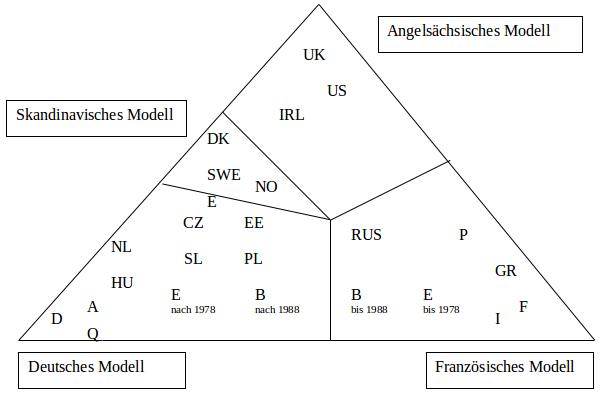
\includegraphics[width=5in]{Material/VerwaltungsModelle}
  \caption{Quelle: Lippert/Umbach 2005 \cite{lipumb05}: 68}
\end{figure}

Aus dem Überblick wird erkennbar, dass es in der EU kein gemeinsames Modell gibt, nach dem eine öffentliche Verwaltung organisiert ist. Vielmehr gibt es nach dieser Darstellung vier Haupttraditionen, die eng mit der historischen Entwicklung in den einzelnen Ländern verbunden sind. Dass die Orientierung in eine bestimmte Richtung nicht statisch ist, zeigen die Beispiele Belgien und England, deren Administrationen zunächst dem französischen Modell angelehnt waren und nun eher dem deutschen Modell folgen, wie im obigen Schema ersichtlich. Weiterhin unterliegen die öffentlichen Verwaltungen Einflüssen, die aus einer generellen Internationalisierung resultieren. So hat das Konzept des „New Public Management“ in allen EU-Mitgliedstaaten zu einem Umdenken und vielfach auch Umbau der Verwaltungen geführt (vgl.\cite{dunhoo}).
\par
Die Modernisierung der öffentlichen Verwaltung ist weltweit in fast allen Ländern zum Thema geworden. In vielen Ländern auf allen Kontinenten sind Aktivitäten zu verzeichnen, deren Ziel eine rationale und effektive Verwaltungsführung ist. Damit verbunden ist meist die Hoffnung auf Kosteneinsparungen, die konsequente Trennung von Verwaltung und Politik, größere Bürgernähe der Verwaltung und/oder verbesserte Aufgabenerfüllung der öffentlichen Hand. Dabei sind mehrere Beweggründe für Verwaltungsmodernisierung zu beobachten:
\par
\begin{itemize}
\item In Ländern mit entwickelten öffentlichen Verwaltungen die Notwendigkeit, Ausgaben im öffentlichen Sektor einzusparen.
\item In Transformationsländern mit nicht existenten Verwaltungsstrukturen oder vormals Kommandowirtschaft die Notwendigkeit, Verwaltungsstrukturen nach modernen Kriterien aufzubauen.
\item Internationale Ausrichtung, z.B. EU-Mitgliedschaft.
\item Globalisierung: Wettbewerb der Länder untereinander bei der Schaffung optimaler Bedingungen für global operierende Unternehmen und Investoren.
\end{itemize}
Man kann zwei Phasen unterscheiden bei dem Austausch von Erfahrungen zwischen Ländern im Feld öffentlicher Verwaltung. Die erste Phase bestand ungefähr von den 1970er Jahren bis Ende des 20. Jahrhunderts. Diese Phase war geprägt von Informalität, Spontaneität und Freiwilligkeit. Kennzeichen war die gegenseitige Beeinflussung der administrativen Systeme, basierend auf Verwaltungsrecht und Gewohnheitsrecht, sowohl in Europa als auch in der Welt. Die zweite Phase des Austausches von Erfahrung und Wissen im Bereich öffentlicher Verwaltung ist seit Beginn des 21. Jahrhunderts auszumachen. Die Überzeugung, dass man die nationalstaatlichen öffentlichen Verwaltungen nicht nur sich selbst überlassen sollte, wurde in der Milleniumserklärung der Vereinten Nationen 2000 in den Blick genommen, die die enge Verzahnung des Kampfes gegen Armut und das Recht auf Entwicklung und „Good Governance“ definierte. 
\subsection{Das Konzept „Good Governance”}
In der vorliegenden Arbeit wird der Begriff „Reform der öffentlichen Verwaltung“ (Englisch: Public Administration Reform, PAR) in einem umfassenden Sinne verstanden; er umfasst den Beamtenapparat, seine rechtliche Verankerung, seine Funktionen, Kompetenzen und Verfahren, unter Einschluss der Verwaltung des Justizsystems. Über den klassischen Begriff der öffentlichen Verwaltung hinaus wird ein umfassenderes Konzept von ‘governance’ zugrunde gelegt. Dieses schließt die Kultur des Regierungshandelns im Sinne der nationalen Entscheidungen hinsichtlich der Ausgestaltung von Staatlichkeit (Legitimität, Effektivität, Transparenz, Pluralität und Verantwortlichkeit) ein, ebenso wie die Beziehungen zwischen Regierung und Parlament.\par
Der Begriff Governance, der zentral ist in der Betrachtung der Verwaltungsmodernisierung in den Ländern, die einen EU-Beitritt anstreben, wird von verschiedenen Institutionen unterschiedlich beschrieben.\par
Die Vereinten Nationen gehen von einer umfassenden Definition von „Governance“ aus, die die Definition einer modernen öffentlichen Verwaltung einschließt. „Governance“ im Gegensatz zum traditionellen Verständnis von „Öffentlicher Verwaltung“ legt einen Schwerpunkt auf Mitgestaltung und Partnerschaft. „Public administration needs to be transformed into a responsive instrument to meet the needs of all citizens“ (\cite{unpan}).\par
Das gewachsene Interesse an einer Governance-Orientierung der Vereinten Nationen wird auf folgende Entwicklungen zurückgeführt:
\begin{itemize}
\item den Erfolg der Marktwirtschaft und das Scheitern der Planwirtschaft;
\item die Tendenz, demokratische Regierungsformen mit wirtschaftlichem Erfolg gleichzusetzen;
\item die weltweite Krise der öffentlichen Finanzen, die in vielen Staaten die Frage nach der Rolle und der Effizienz des Staates neu gestellt hat; 
\item die gestiegene Wahrnehmung und Verärgerung über Korruption in Regierung und Verwaltung;
den Zusammenbruch der ehemaligen Sowjetunion und die ethnischen Konflikte auf dem Balkan und in Afrika, die die neuen Staaten vor große Umbauaufgaben auch ihres politischen Systems stellen (vgl. \cite{undp}: 18).
\end{itemize}
Die Weltbank beschreibt das Konzept als “the traditions and institutions by which authority in a country is exercised for the common good” (\cite{weltbank}: 1). Die sechs Governance-Indikatoren der Weltbank gelten mittlerweile als Standardkriterien zur Bewertung von Good Governance: 
\begin{itemize}
\item Politische Mitspracherechte (Voice and Accountability),
\item Politische Stabilität und Gewaltkontrolle (Political Stability and No Violence);
\item Effektivität des Regierens (Government Effectiveness),
\item Qualität regulativer Politik (Regulatory Quality),
\item Rechtsstaatlichkeit (Rule of Law),
\item Korruptionskontrolle (Control of Corruption) (vgl. \cite{kaufmann}).
\end{itemize}
Im Laufe der 1990er Jahre übernahmen auch die in der OECD zusammengeschlossenen Geber sowie die EU das Konzept der „guten Regierungsführung“.\par
Die SIGMA-Initiative der OECD versucht in ihrer Veröffentlichung zu ‘European Principles of Public Administration’ im Jahr 1999, ebenfalls an den Weltbankindikatoren angelehnt, Prinzipien für die öffentlichen Verwaltungen in ihren Mitgliedstaaten aufzustellen. Folgende Indikatoren werden genannt: 
\begin{itemize}
\item reliability and predictability (legal certainty or judicial security); 
\item openness and transparency; 
\item accountability; 
\item efficiency and effectiveness (vgl. \cite{oecd99}: 8ff).
\end{itemize}
An dem Good-Governance-Verständnis von Weltbank und IWF sowie OECD orientiert sich auch die Europäische Union. Die Europäische Kommission hat im Jahr 2001 ihr Weißbuch „Europäisches Regieren“ veröffentlicht, das ebenfalls Kriterien guter Regierungsführung enthält (vgl. \cite{czada2010}). Dort werden folgende Prinzipien als Merkmale von Good Governance definiert:
\begin{itemize}
\item Transparenz: Institutionen sollten in ihrem Handeln transparent sein und erklären, wie ihre Entscheidungen zustande kommen.
\item Partizipation: Die Qualität und Effektivität von Politik hängt wesentlich von umfassender Partizipation ab.
\item Übernahme von Verantwortung: Institutionen müssen erklären, warum sie etwas tun, und auch dafür Verantwortung übernehmen.
\item Effektivität: Policies müssen effektiv und zeitnah umgesetzt werden mit dem Ziel, das Benötigte auf der Basis von definierten Zielen zu liefern.
\item Kohärenz: Policies und Handlungen müssen kohärent und nachvollziehbar sein.
(vgl. \cite{euko01}: 13).
\end{itemize}
Gute Regierungsführung ist demnach im Wesentlichen gleichbedeutend mit einer leistungsfähigen, berechenbaren und transparenten staatlichen Verwaltung. Sie setzt „ein funktionierendes öffentliches Buchführungs- und Rechnungswesen ebenso voraus wie einen verbindlichen rechtlichen Rahmen, der privatwirtschaftlichen Wettbewerb ermöglicht“ (\cite{schmitz09}: 132).
\par
In der Debatte um die Notwendigkeit stabiler Institutionen und einer effektiven öffentlichen Verwaltung schwingt explizit oder implizit mit, dass die Modernisierung der öffentlichen Verwaltung die Demokratisierung vorantreibt. „Die Demokratie ist heute eigentlich keine Volksregierung, sondern eine Volksverwaltung – die Administration ist die eigentliche Aufgabe der Demokratie“ (Masaryk, zit. nach \cite{czerwick}: 14). Czerwick merkt dazu an, dass in der wissenschaftlichen Literatur davon ausgegangen wird, dass demokratische Systeme nur überleben können, wenn sichergestellt ist, dass die öffentlichen Verwaltungen ein Mindestmaß an struktureller Übereinstimmung mit demokratischen Normen, Institutionen und Prinzipien aufweisen.
\par
Vor diesem Hintergrund ist im Zusammenhang mit der (weiteren) Demokratisierung der Staaten des Westlichen Balkans und ihrem Wunsch einer Aufnahme in die Europäische Gemeinschaft die Frage nach dem Status quo der Verwaltung in diesen Ländern unumgänglich. Es wird deutlich, dass die öffentliche Verwaltung ein zentrales Element ist für die weitere Entwicklung, Demokratisierung und ultimativ den EU-Beitritt der Balkanstaaten. Dennoch ist dieser Zusammenhang von der Forschung bislang wenig beachtet worden. Die vorliegende Arbeit versucht erste Schritte, um diese bemerkenswert große Forschungslücke zu schließen. In Anbetracht der kaum vorhandenen Literatur wird das Thema Verwaltungsmodernisierung im Westbalkan im Kontext der EU-Erweiterung in der vorliegenden Arbeit von mehreren Seiten betrachtet. Die historische Perspektive fließt mit ein, in der Hoffnung auch aus dieser Betrachtung Hinweise zur Beantwortung der Forschungsfragen zu erhalten.
\section{Methodisches Konzept}
In der vorliegenden Arbeit wird eine Annäherung an ein bisher weitgehend nicht untersuchtes Thema, die Bedeutung der Reform der öffentlichen Verwaltung im Westlichen Balkan im Kontext der EU-Erweiterung, vorgenommen. Da mit dieser Untersuchung quasi Neuland betreten wird, wurde eine Methode gewählt, die es ermöglicht, das Thema von unterschiedlichen Seiten aus zu betrachten. Gewählt wurde ein kaleidoskopisches Verfahren, mittels dessen versucht wird, Antworten auf die zentrale Frage und die weiterführenden Fragen der Untersuchung finden. Die Vorgehensweise in der vorliegenden Arbeit ist im Rahmen des Forschungsansatzes der Triangulation verortet. Triangulation findet vor allem in der empirischen Sozialforschung Anwendung. Mit unterschiedlichen Methoden oder Sichtweisen, bzw. Daten wird versucht ein Phänomen zu erklären. Ursprünglich kommt der Begriff Triangulation aus der Landvermessung, wo er folgendermaßen verwendet wird:\par
„Triangulation is the method of location of a point from two others of known distance apart, given the angles of the triangle formed by three points. By repeated application of the principle, if a series of points form the apices of a chain or network of connected triangles of which the angles are measured, the lengths of all the unknown sides and the relative positions of the points may be computed when the length of one of the sides is known” (\cite{clark}: 145).\par
In der sozialwissenschaftlichen Forschung wurde die Triangulation als Methode entwickelt, um von verschiedenen Referenzpunkten aus die Position des (Forschungs-)Objektes zu lokalisieren (vgl. Smith 1975, zit. nach \cite{jick}: 136). Auf dieser Grundlage definiert Flick: „Triangulation beinhaltet die Einnahme verschiedener Perspektiven auf einen untersuchten Gegenstand oder allgemeiner: bei der Beantwortung von Forschungsfragen. Diese Perspektiven können sich in unterschiedlichen Methoden, die angewendet werden, und/oder unterschiedlichen gewählten theoretischen Zugängen konkretisieren, wobei beides wiederum miteinander in Zusammenhang steht bzw. verknüpft werden sollte. Weiterhin bezieht sie sich auf die Kombination unterschiedlicher Datensorten jeweils vor dem Hintergrund der auf die Daten jeweils eingenommenen theoretischen Perspektiven“ (\cite{flick08}:12).\par

In ähnlicher Weise resümiert Schirmer: „Triangulation meint – allgemein gesprochen – die Betrachtung eines ‚Punktes’ aus mehreren Perspektiven mit dem Ziel, diesen Punkt umfassender oder vollständiger zu verstehen, sozusagen ein kompletteres Bild zu entwerfen; damit sollen gleichzeitig Verzerrungen oder Fehlblicke vermieden oder relativiert werden, die Resultat einer bestimmten Perspektive sind.“ (\cite{schirmer}: 100). \par
Der Kern der Triangulation als Methode in der sozialwissenschaftlichen Forschung ist die Kontrastierung. In der vorliegenden Arbeit werden die Erkenntnisse aus der Literaturanalyse anhand von Interviews mit Experten überprüft und so eine Kontrastierung vollzogen, die möglicherweise zu neuen Erkenntnissen und weiterführenden Fragestellungen führt. Diese Vorgehensweise erscheint als eine gute Grundlage für weitergehende Forschung zu dem bisher wenig beleuchteten Thema dieser Arbeit.\par

In der praktischen Anwendung kann man zwei unterschiedliche Lesarten zu Triangulation feststellen. Im ersten Fall wird die Triangulation als Validierung von Forschungsergebnissen durch die Verwendung unterschiedlicher Methoden gesehen. Eine andere Lesart ist die Triangulation mit dem Ziel, ein umfassenderes Bild des Gegenstandsbereichs zu erzielen und den Untersuchungsgegenstand von unterschiedlichen Perspektiven her zu betrachten (vgl. \cite{kelle}: 50). Für die vorliegende Untersuchung wird die Triangulation im letzteren Sinne verwandt.
\par
Es wird versucht, über eine Betrachtung der historischen Verwaltungstradition und Verwaltungsentwicklung in drei benachbarten Ländern des Westlichen Balkans (Albanien, Mazedonien und Montenegro) Gemeinsamkeiten und Unterschiede aufzuspüren, die für den Status quo der Verwaltungsentwicklung in den Ländern relevant sein könnten.\par
Der aktuelle Bezugspunkt der Untersuchung und allen drei Untersuchungsländern gemein ist die Aufnahmeperspektive in die EU. Neben der Entwicklung der Beziehungen der Untersuchungsländer zur EU wird daher auch die Unterstützung der EU im Rahmen der Heranführungshilfe für die Aufnahmekandidaten beschrieben.\par
In einem weiteren Teil der Arbeit werden von der Verfasserin durchgeführte Experteninterviews zu den Forschungsfragen der Arbeit ausgewertet. Die Interviews betreffen thematisch den Status quo der Verwaltungsmodernisierung in den Untersuchungsländern und die Unterstützung durch die EU. Sechs Interviews wurden hierzu mit hochrangigen Beamten der EU und OECD / SIGMAs durchgeführt. Um die Perspektive in den Untersuchungsländern zu erfassen, wurden außerdem in jedem der drei Länder jeweils ein Vertreter der Regierung und ein Vertreter einer Nichtregierungsorganisation (NRO/NGO) interviewt. Alle Interviewpartner waren intensiv mit Verwaltungsmodernisierung befasst und sind in diesem Sinne Experten zum Thema. Insgesamt wurden also zwölf Interviews durchgeführt, die für die vorliegende Arbeit ausgewertet wurden.
\par
In Anbetracht der noch sehr überschaubaren Literatur zum Prozess der Verwaltungsmodernisierung in den Westbalkanländern unter dem Einfluss des EU-Erweiterungsprozesses stellt die Auswertung der Experteninterviews einen unverzichtbaren Beitrag dar. Dabei geht es nicht vorrangig um die Validierung von Ergebnissen der Literaturdurchsicht, sondern um eine Erweiterung der Forschungsperspektive unter Einschluss der persönlichen Erfahrungen und Meinungen von Experten, die sich mit dem Thema in der täglichen Berufspraxis beschäftigten.\par
In die vorliegende Untersuchung fließen ferner Eindrücke aus der eigenen beruflichen Praxis ein. Die Verfasserin hat mehrere Jahre für die OSZE in Südosteuropa im Bereich Demokratisierung vor allem in der Durchführung und Beobachtung von Wahlen gearbeitet (Kosovo noch unter internationaler Administration, Bosnien-Herzegowina, Albanien und Montenegro). Ein wiederkehrender Befund durchzieht diese jahrelange Beschäftigung. Einerseits handelt es sich bei dieser Region geografisch um Europa. Im gemeinsamen Land Jugoslawien bestanden über viele Jahre politisch und ökonomisch enge Kontakte mit den Ländern der EU und der EU als Institution. Andererseits erscheint die Region heute weit von Europa entfernt. So findet Berichterstattung in den westeuropäischen Medien kaum statt. Dieses mangelnde Interesse kann nur zum Teil mit den Kriegen Anfang der 90er Jahre erklärt werden, die zu ökonomischen und politischen Rückschritten führten.\par
Der Widerspruch zwischen einerseits geografischer Zugehörigkeit zu Europa und andererseits wahrnehmbar großer Entfernung zu Westeuropa spiegelt sich auch in der Herangehensweise der EU gegenüber der Region. Einerseits hat die EU den Staaten des Westbalkans seit 2003 einen Beitritt zur EU in Aussicht gestellt. Andererseits sind Auflagen seitens der EU formuliert worden, die in wesentlichen Punkten über die Anforderungen der früheren Aufnahmewellen hinausgehen. Auch wird die bisher gängige Praxis einer gemeinsamen EU-Aufnahme mehrerer Staaten für die Länder des Westbalkans ausgeschlossen.
\section{Aufbau der Arbeit }
Übergeordneter Bezugsrahmen für die vorliegende Arbeit ist zunächst die Konditionalität der EU, die derzeit den theoretischen Hauptstrang der Europäisierungsforschung darstellt. Das Konzept der Konditionalität wird im zweiten Kapitel aus der Demokratisierungs- und Transformationsforschung hergeleitet und bildet den ersten Rahmen der Untersuchung.
Ebenfalls im zweiten Kapitel wird der Prozess der EU-Erweiterung in der Praxis dargestellt. Dabei wird auch ausführlich auf den Stellenwert der Verwaltungsmodernisierung in diesem Prozess eingegangen. Hierbei ist zentral, dass Verwaltungsentwicklung im Erweiterungsprogramm der EU nicht explizit vorkommt. Eine implizite Bezugnahme ist dennoch erkennbar mit dem Konzept des Europäischen Verwaltungsraums, das ebenfalls dargestellt wird. Für dieses Kapitel werden Veröffentlichungen der EU und anderer internationaler Akteure (OECD/SIGMA, UNDP, Weltbank usw.) hinsichtlich des Stellenwertes von Verwaltungsentwicklung innerhalb des Erweiterungsprozesses ausgewertet. Ein wichtiger Teilaspekt der Betrachtung in diesem Kapitel ist die Auswertung der letzten Aufnahmewelle der EU hinsichtlich der Erfahrungen mit und der Nachhaltigkeit von Verwaltungsmodernisierung. Abschließend werden im zweiten Kapitel die Hilfen der EU für die Verwaltungsentwicklung in Kandidatenländern vorgestellt. \par
Die Ausgangslage auf dem Westbalkan ist Gegenstand des dritten Kapitels und bildet einen weiteren Rahmen für die Arbeit. Es wird auf die sozialistische (Jugoslawien) und kommunistische (Albanien) Verwaltungsgeschichte ebenso eingegangen wie auf die zeitlich davor gelagerten imperialen Einflüsse auf die Verwaltung (Österreich-Ungarn, Osmanisches Reich). Dieser Teil der Arbeit wird vorwiegend mittels einer Literatur-Auswertung durchgeführt. Auch die Sichtung von Akten der Österreichischen Militärverwaltung in Montenegro und Albanien während des Ersten Weltkrieges durch die Autorin im Staatsarchiv in Wien fließt in diesen Teil der Untersuchung ein. Als Bezugsrahmen dieses Teiles der Arbeit dient der Legacy-Ansatz, der auch für die vergleichende Verwaltungsforschung anwendbar ist. An die historische Betrachtung schließt sich die kursorische Darstellung der Verwaltungsentwicklung in den drei Untersuchungsländern in der Demokratie an.
\par
Der empirische Teil der Arbeit folgt im vierten Kapitel, bestehend aus zwölf Experteninterviews. Im ersten Teil dieses Kapitels wird die angewandte Methode für die Durchführung der Experteninterviews dargestellt, einschließlich des Vorgehens bei der Auswertung. Im Hauptteil des vierten Kapitels werden die Ergebnisse der Experteninterviews analog der behandelten Themenstränge dargestellt und analysiert.\par
Das Gesamtergebnis der Untersuchung wird im fünften Kapitel zusammengefasst dargestellt.
%\chapter{Forschungsansätze zum politischen Wandel in Europa }
Prozesse des politischen Wandels sind weltweit mit unterschiedlicher Intensität und aufgrund verschiedenartiger Impulse unter dem Einfluss unterschiedlicher Rahmenbedingungen zu beobachten. Schwerpunkte sind die Umwandlung traditionell regierter Länder zu modernen Staaten, wie insbesondere im Rahmen der westlichen Entwicklungshilfe, und aktuell die Umwälzungen in Nordafrika, sowie die Transformation vormals sozialistisch beherrschter Länder in demokratisch regierte Staaten in Osteuropa. Die Aufnahme von Staaten in die Europäische Union stellt für diese ebenfalls einen grundlegenden Wandel dar, zu dessen Beschreibung und Gestaltung allgemeine Forschungsergebnisse aus den verschiedenen Prozessen des politischen Wandels herangezogen werden können. Die Forschungsrichtung der Europäisierungsforschung und hier insbesondere das Konzept der Konditionalität ist der vorherrschende Ansatz zur Erklärung verschiedenster Prozesse, welche die EU als supranationale Organisation entfaltet. Die Europäisierungsforschung wird in diesem Kapitel als zentraler Ansatz ausführlich dargestellt, insbesondere die in ihrem Umfeld entwickelte Konditionalitätsforschung. Diese Forschungsrichtung ist von besonderer Bedeutung für die vorliegende Arbeit, da die Verwaltungsmodernisierung ein wesentliches Element der EU-Bedingungen für die Aufnahme der Westbalkanstaaten ist. Im Folgenden werden diese Forschungsrichtungen aus der Transitionsforschung hergeleitet mit den konkreten Fragestellungen der Europäisierungsforschung und der Konditionalitätsforschung. 
\section{Transitionsforschung}
Die Transitionsforschung, die sich traditionell mit Entwicklungsländern beschäftigte, erfuhr durch die politische Wende in Osteuropa eine neue Ausrichtung. Nach dem Systemwechsel in den Ländern Mittel- und Osteuropas war die wissenschaftliche Aufarbeitung der Geschehnisse zunächst von wirtschaftswissenschaftlichen Konzeptionen beherrscht, die sich vor allem mit dem Wechsel der Wirtschaftsweise von zentraler Planwirtschaft zu Marktwirtschaft befassten. Die auch stattfindenden politischen Transformationsprozesse wurden in der Folge ebenfalls nach und nach mit Erklärungsmodellen begleitet. Es entstanden Staatenanalysen und Untersuchungen spezifischer Systembereiche mit ökonomischem, demokratietheoretischem oder soziologischem Schwerpunkt (\mbox{vgl. \cite{huszak}: 54ff}).\par
König definiert den Prozess der Transition in den neu entstandenen Ländern Osteuropas eher als einen der Transformation. „It is evident that in the transition from command to market economy and from totalitarian state to a pluralist state, creating multiparty democracy is not only a transition in itself but rather a long process of transformation. It requires essential reforms in the basic functions and institutions of the state” (König 1992, zit. nach \cite{jenei}). \par
Der Einfluss der EU als einer der wesentlichen Geber kam zunehmend in den Blick als externer Akteur der Transformation. Von Beyme konstatiert in diesem Zusammenhang, dass der „internationale Einfluss der etablierten Demokratien auf die neuen Systeme (…) eine neue Dimension in der Weltgeschichte“ darstellt (\cite{beyme}: 158). Whitehead geht von drei Formen der Demokratisierung aus, erstens der auferlegten Demokratisierung, zweitens Demokratisierung durch Dekolonisierung und drittens Demokratisierung durch Konvergenz (vgl. \cite{whitehead}). Pridham entwickelt ein Konzept der interaktiven Prozesse zwischen externen (vor allem internationalen Organisationen) und innerstaatlichen Akteuren (vgl. \cite{pridham91,pridham95,pridham08}), während das Konzept der Diffusion bzw. einer Art „Schneeballeffekt“ bei der Demokratisierung von Huntington stammt (vgl. \cite{hunting}). Eine Aufarbeitung des Systemwandels in Osteuropa unter Betrachtung externer Faktoren findet statt; diese werden allerdings noch nicht in einem ausreichenden Maße in theoretische Erklärungszusammenhänge eingebunden: „…even though the influence of international factors has been widely acknowledged, these still have not been fully integrated into theoretical frameworks aiming to explain the dynamics or failure of post communist transitions“ (\cite{dimpri}: 93).\par
Im Rahmen der Transitionsforschung wird der Erkenntnis, dass der Beitritt zur EU spezifische Transformationsergebnisse zeitigt, zunehmend Raum gegeben. Die Forschung zum Institutionenwandel zentralstaatlicher Administration in nachkommunistischen Ländern im Rahmen der Transformations- und Integrationsforschung ist dagegen noch eher unterentwickelt. Nur selten wird auf die Entwicklung der Ministerialbürokratien und Regierungen in einem engeren Sinne Bezug genommen. Insbesondere Probleme mit der administrativen Kapazität der neuen Mitgliedsländer werden, so Lippert und Umbach, lediglich auf allgemeine Weise abgehandelt. “Therefore, the cross-country research on the administrative developments under the pressure of Europeanisation is particularly relevant” (\cite{lipumb05}: 17). Auch Luchterhand konstatiert schon 2001 im Vorwort seiner Analyse zu Verwaltung und Verwaltungsrecht im Erneuerungsprozess Osteuropas: „Dass die tatsächliche Erfüllung der Beitrittsvoraussetzungen – unterhalb einer demokratischen und menschenrechtskonformen Verfassung – nicht nur von einem EU-kompatiblen Wirtschaftssystem abhängt, sondern kaum weniger von einer leistungsstarken und rechtsstaatlich fundierten öffentlichen Verwaltung, hat man daneben weithin kaum zur Kenntnis genommen“ (\cite{lucht}: 6).\par
Die Transitionsforschung mit ihrer Untersuchung des politischen Wandels ist für die vorliegende Arbeit besonders fruchtbar. Im Zuge der EU-Erweiterung kam auch die EU als externer Akteur mit Einfluss auf Beitrittsländer in den Blick der Transitionsforschung. Die Betrachtung des Institutionenwandels als erklärtem Ziel dieser Forschungsrichtung bietet sich somit auch für die Betrachtung der Verwaltungsentwicklung an. 
\section{Neo-Institutionalismus als Ansatz zur Erklärung des Wandels}
Der Neo-Institutionalismus, der von einer zentralen Bedeutung der Institutionen für soziales Handeln ausgeht, kann als Gegenbewegung zu dem in den USA seit den 1960er Jahren dominanten „Behaviouralismus“ betrachtet werden. Dieser versuchte politische Phänomene vor allem über individuelle Einstellungen und individuelles Verhalten zu erklären. Ausgangspunkt der Kritik an einem rein verhaltenswissenschaftlichen Erklärungskonzept war die fehlende Erfassung der wachsenden Bedeutung von Institutionen. Der Zusammenbruch der Staaten in Ost- und Mitteleuropa und die damit einsetzende Erforschung der Transformationsprozesse brachte die Institutionen erneut in den Blick. Die zunächst vorherrschende Einschätzung, dass in diesen Ländern im Wesentlichen eine „nachholende Modernisierung“ stattfindet, wurde angesichts wirtschaftlicher Probleme und ethnischer Auseinandersetzungen zunehmend fragwürdig. Die Sichtweise verschob sich zunehmend hin zur Annahme, dass die Wandlungsprozesse nicht in logischer Folge ablaufen, sondern dass man von Prozessen ausgehen muss, die geprägt sind von Verteilungskämpfen und traditionellen institutionellen Einflüssen. So „finden sich in den Gesellschaften Ost- und Mitteleuropas zahlreiche so genannte institutionelle Hinterlassenschaften (institutional legacies), d.h. Routinen, Regeln und soziale Bindungen, die den Verlauf der Transformation maßgeblich beeinflussen“ (\cite{schulze}: 5). Es wird also nach der Veränderung des institutionellen Gefüges durch Anpassungsprozesse unterschiedlichster Art und Geschwindigkeit gefragt. \par
Im „neuen“ Institutionalismus in der Politikwissenschaft, der seit den 1970er Jahren verstärkt zum Einsatz kommt, unterscheidet man im Wesentlichen drei Varianten.\par
Erstens gibt es eine stark vom Rational-Choice-Ansatz bestimmte Richtung, die sich mit der Wirkung politischer Institutionen in den verfassungsmäßigen Entscheidungsgremien befasst.
In Rational-Choice-Ansätzen ist das politisch-soziale System Untersuchungsgegenstand. Grundlage für die Analyse ist das Konzept des methodologischen Individualismus, wonach Entscheidungen immer nur von weitgehend rational handelnden Individuen getroffen werden können und somit Handlungen von Kollektiven (z.B. Behörden) eine Anhäufung von Einzelfallentscheidungen seien. Dabei werden strukturelle Faktoren weitgehend ausgeblendet bei vorwiegender Berücksichtigung der angenommenen Interessen der beteiligten Akteure. Putnam entwickelt für den Blick auf die europäische Integration ein Zwei-Ebenen-Modell. Er geht davon aus, dass bei Verhandlungen über internationale Kooperationen gesellschaftliche Akteure auf nationaler Ebene Druck auf die Regierung ausüben, um ihre Ziele zu realisieren. Gleichzeitig werden von den nationalen Regierungen die Verhandlungen auf internationaler Ebene genutzt, um den Erwartungen der einheimischen Akteure nachzukommen bzw. zu entkommen (vgl. \cite{putnam}). Kritik an den akteursorientierten Ansätzen zielt vor allem auf die mangelnde Berücksichtigung struktureller und institutioneller Rahmenbedingungen ab.\par
Zweitens gibt es eine kulturalistisch-konstruktivistische Variante, die sich vom Rational-Choice-Modell abgrenzt. Hierfür steht der Ansatz von March und Olsen. Diese definieren Institutionen als ein Gefüge aus Regeln und Verhaltensroutinen, die durch soziale Werte und Normen bedingt sind und so die Akteursreaktionen beeinflussen. Es können daher kaum identisch ausgeprägte Institutionen bei unterschiedlichen kulturellen und sozialen Rahmenbedingungen entstehen (\mbox{vgl. \cite{marols}: 17}).\par
Drittens gibt es die vermittelnde Variante des sogenannten historischen Institutionalismus. (\cite{haltay, steinmo}). Die Wirkung von Institutionen wird historisch sowie national und sektoral vergleichend untersucht. Der historisch-soziologische Ansatz entspringt der vergleichenden Regierungslehre und stellt den Staat als zentralen Akteur mit seinen Machtpotenzialen in den Mittelpunkt.\par
Im Zentrum der Untersuchungen im Rahmen des Neo-Institutionalismus stehen die Beweggründe für institutionelle Änderungen und die Frage, wie die neuen Spielregeln nach Überwindung der alten Regeln und Handlungsmuster verfestigt und angenommen werden. Vor allem die Mechanismen des Wandels sind im Blick sowie der Einfluss des veränderten Umfelds auf die Politikgestaltung (\mbox{vgl. \cite{huszak}}).\par
Kennzeichnend für die aktuellen Forschungen nach den neo-institutionalistischen Konzepten ist die Konzentration auf die Bedeutung der Institutionen bei der Betrachtung gesellschaftlichen Wandels. Dies geschieht insbesondere in Abgrenzung zu verhaltenswissenschaftlichen Erklärungsansätzen, die in den Sozialwissenschaften in den USA seit den 1960er Jahren vorherrschend waren. Die Europäisierungsforschung kann als eine Weiterentwicklung der neo-institutionellen Theorien gesehen werden. \par
Auf Basis der bisher dargestellten Ansätze zum politischen Wandel wird zunächst die Europäisierungsforschung näher beleuchtet; diese stellt eine weitere Konkretisierung der Transitionsforschung im Zusammenhang mit der EU-Erweiterung dar. In einem weiteren Schritt wird auf eine Unterkategorie der Europäisierungsforschung, die Konditionalitätsforschung, eingegangen. Forschungen zur Konditionalität haben insbesondere in Bezug auf die politischen Kriterien im Erweiterungsprozess Relevanz. Die Verwaltungsentwicklung in den Beitrittsländern wird von der EU nach politischen Kriterien betrachtet. 
\section{Europäisierungsforschung}
Die Rolle der EG/EU im Zusammenhang mit Demokratisierung war im Prinzip vor 1989 nicht im Blick der Forschung und auch anlässlich der Süderweiterung (überraschenderweise) nicht beleuchtet worden (vgl. Kneuer 2007). Bezogen auf Mittel- und Osteuropa beschäftigte sich die Europaforschung vor allem mit den technischen Aspekten der Assoziierung (Europaabkommen) im Rahmen des Heranführungs- und Beitrittsprozesses (\cite{lipbec, lipsch}). Weiterhin wurden die sich entwickelnden Beziehungen zwischen der EU und den Beitrittsländern thematisiert (\cite{mayhew, torre}). Die klassische Integrationsforschung beleuchtete vor allem, ob und wie die Mitgliedstaaten auf die Entwicklung supranationaler Institutionen und Politiken einwirkten. Ein Perspektivwechsel seit Mitte der 1990er Jahre führte zur zunehmenden Beschäftigung mit der Frage nach dem Einfluss der EU und den Effekten auf nationale Systeme (vgl. \cite{kneuer09}: 21). Damit war der Paradigmenwechsel vollzogen und die nun Europäisierungsforschung genannte Betrachtungsweise basierte auf der These, dass die EU unterschiedliche Effekte in den Mitgliedstaaten hervorrufen kann. Die einsetzende Theoriebildung versuchte den Einfluss und die Wirkung der EU auf die Mitgliedstaaten und die dort ablaufenden Prozesse, Politikinhalte, Einstellungen und Normen zu beschreiben (\cite{boerzel, boeris00, radaelli00, kohler, fearad03}). Es wurde der Frage nachgegangen, ob die EU zu policy-Veränderungen führt, zur Transformation von Institutionen, oder sogar zu Identitätsveränderungen (\cite{meny, knilen, fearad03, boeris07}). \par


Im Allgemeinen wird unter Europäisierung das Zusammenwirken der folgenden drei Zusammenhänge verstanden: 
\begin{itemize} \itemsep1pt \parskip0pt \parsep0pt
\item Die Herausbildung und Entwicklung spezifischer Strukturen von „Governance" auf europäischer Ebene (vgl. \cite{risseetal}: 3, \cite{radpas}: 36).
\item Europäisierung als „top-down“-Prozess, der durch Institutionen und Entscheidungen auf der Ebene der EU die nationalen policies und Institutionen formt (vgl. \cite{herit}).
\item Ein Prozess mit folgenden Schritten: a) Konstruktion, b) Diffusion und c)~Institutionalisierung von Normen, Glaubenssätzen und informellen Regeln, Abläufen, policy-Paradigmen, Stilen und „der Art wie Dinge getan werden“. Diese sind zunächst durch den EU-policy-Prozess definiert, werden dann auf die nationale Ebene übertragen und in die öffentlichen Debatten, politischen Vorgaben und Institutionen übernommen. Diese letzte Beschreibung basiert auf der Annahme der Europäisierung als Institutionalisierung und interaktivem Prozess, der über einen ein-direktionalen Mechanismus als Reaktion auf Europa und auch über das Konzept des „impact“ oder Einflusses der EU auf nationale Systeme hinausgeht. Damit ist keine vertikale Anpassung gemeint, sondern ein Sozialisierungsprozess im umfassenden Sinne (\mbox{vgl. \cite{fearad03, olsen}}).
\end{itemize}
Der letztgenannte Ansatz betrachtet unter verschiedenen Blickwinkeln und in einer diskursiven Herangehensweise, wie nationale Veränderungen geschehen. Zwar kann man mit definierten Kriterien den Grad der Europäisierung messen oder zumindest beschreiben, allerdings ist ein besonderes Problem immer die Abgrenzung von Anpassung und Transformation (\mbox{vgl. \cite{radpas}: 40}).\par
Die klassischen Probleme der Forschung zur Europäisierung sind a) Voreingenommenheit bei der Beurteilung des Einflusses der EU auf die nationalen policies und die Politik und b) die Annahme, dass es sich bei nationalen Veränderungen, die den Brüsseler Vorschlägen ähnlich sind, um Europäisierung handelt (vgl. \cite{radpas}: 40). Oder wie Goetz warnt: „Europeanization can very easily become a cause in the search of an effect (at the domestic level)” (\cite{goetz01a}: 211). Noch kritischer wird von Mair angemerkt: „Europeanization and globalization are becoming catch-all, default explananda for almost everything that cannot otherwise be explained at the domestic level” (\cite{mair}: 339).\par
Die Konzepte der Europäisierung wurden zunächst fast ausschließlich auf Mitglieder der EU angewandt. Erst seit der letzten Erweiterungswelle gibt es Studien, die sich im Rahmen der Europäisierungsforschung auch mit Regionen außerhalb der Grenzen der EU beschäftigen (\cite{lipumwes, grab03, papadi, lavenex, schsed05b, schsed05c}). Die aktuellen Ansätze der Europäisierungsforschung sind für empirische Studien vor allem in drei Richtungen nutzbar gemacht worden: Europäisierung als Policy-Veränderung, Europäisierung als Institutionenveränderung sowie Europäisierung und EU-Erweiterung. Diese drei Stränge der Europäisierungsforschung werden im Folgenden kurz dargestellt.
\subsection{Europäisierung als Policy-Veränderung}
Eine Reihe von empirischen Studien wurde zur Europäisierung der politischen Institutionen und Entscheidungsprozesse einzelner Staaten oder als Ländervergleiche durchgeführt. Vor allem Frankreich, Deutschland und Großbritannien dienten dabei als Untersuchungsländer. Weiterhin gibt es Untersuchungen zu einzelnen policy-Feldern. Hier wird oft nach der nationalen Umsetzung der EU-Vorgaben in den Mitgliedstaaten gefragt. Studien in dieser Kategorie beschäftigen sich bislang vor allem mit Umweltpolitik, Sozial- oder Regionalpolitik, seltener mit Landwirtschafts-, Gesundheits-, Wettbewerbs- oder Kulturpolitik. Die Themen Außen- und Sicherheitspolitik sowie Justiz- und Innenpolitik waren bislang selten im Forschungsinteresse, mit Ausnahmen bei der Immigrations- und Asylpolitik (vgl. \cite{bulmer07}: 57). Die vorgelegten Studien zeigen, dass der Einfluss der EU im Bereich der Umweltpolitik und der Sozialpolitik zu höheren Standards in den Mitgliedsländern geführt hat, wobei die südlichen Mitgliedstaaten stärker von Veränderung betroffen waren. Auch wurden neue Instrumente der Politikgestaltung übernommen, die z.B. auf einer stärkeren Einbeziehung von verschiedenen sozialen Gruppen basieren oder auf politikfeldübergreifender Kooperation. In Bereichen, in denen die EU großen Einfluss hat und Eingriffe vornehmen kann, ist es dennoch nicht zu einem einheitlichen Politikstil gekommen (vgl. \cite{boeris07}: 486).
\subsection{Europäisierung als Institutionenveränderung }
Studien in diesem Bereich haben sich mit Fragen beschäftigt, inwieweit europäische Prozesse sich auf die Beziehungen zwischen Regierungen, nationalen Bürokratien und administrativen Prozessen, Regulierungsstrategien, Justizstrukturen oder die Beziehungen zwischen Legislative und Exekutive auswirken. Diese Arbeiten kommen zu keinem eindeutigen Ergebnis. Manche Untersuchungen fanden heraus, dass nationale Institutionen dem europäischen Einfluss im Wesentlichen standgehalten haben, während andere Studien davon ausgehen, dass die EU die nationalen Systeme föderalisiert oder pluralisiert habe. Börzel und Risse sehen in diesen Ergebnissen die Kontroverse gespiegelt, ob die EU-Integration den Staat stärkt, schwächt oder transformiert. Für nationale Verwaltungen konstatieren sie, dass diese die Anforderungen der EU erfüllt haben, aber die konkrete Umsetzung unterschiedlich ausfällt und maßgeblich von den schon existierenden Institutionen abhängt. „National administrations have responded to the \mbox{‚demands} of EU membership’ but institutional adaptation differs significantly and is mediated by pre-existing institutions“ (\cite{boeris07}: 487).
\subsection{Europäisierung und EU-Erweiterung }
Die EU-Erweiterung nach Osteuropa bot eine gute Möglichkeit, die Hypothesen der Europäisierungsforschung zu testen. Die Länder Ost- und Mitteleuropas, insbesondere die post-kommunistischen Länder, hatten eine andere historische Einbindung als westeuropäische Demokratien und sie hatten wenig Möglichkeit, selbst Einfluss auf die EU-Politik auszuüben. Diese Länder mussten den Acquis communautaire übernehmen und standen damit unter einem erheblichen Anpassungsdruck. Damit verbunden war die Vermutung, dass sie die EU-Modelle stärker internalisieren aufgrund der Schnelligkeit, mit der sie EU-Vorgaben übernehmen mussten angesichts des großen Umfangs der zu übernehmenden EU-Agenda und dank der größeren Offenheit für EU-Modelle im Rahmen des post-kommunistischen Transformationsprozesses (vgl. \cite{grab03}). Doch die Studien zeichnen kein eindeutiges Bild. Die meisten Forscher stimmen darin überein, dass die EU-Erweiterung den Hauptstimulus darstellte und die Übernahme des Acquis communautaire die Aufnahmebedingung war. Dies bedeutete auch, dass Europäisierung in diesem Zusammenhang eher ein „top-down"-Prozess und eine „Einbahnstraße“ war. Zwar zeigte sich, dass die wesentlichen Verwaltungseinheiten gestärkt wurden, die Entwicklung eines nicht-politisierten civil service begünstigt wurde und ein gewisser Grad an Dezentralisierung erreicht wurde, zumindest im Gegensatz zur kommunistischen Zeit. Dennoch variieren die Auswirkungen auf Institutionen und Politik erheblich.\par
Zusammenfassend kann gesagt werden, dass die Europäisierungsforschung im Rahmen der Transformationsforschung entstanden ist. Zunächst wurde vor allem der Einfluss der EU auf nationale Politik und Institutionen in den Mitgliedsländern untersucht. In der praktischen Anwendung auf unterschiedliche Politikfelder stellte sich heraus, dass vor allem im Bereich der Umwelt- und Sozialpolitik durch Anforderungen der EU insgesamt höhere Standards zur Durchsetzung kamen.
\par
In der vergleichenden Betrachtung zur institutionellen Veränderung durch EU-Politik zeichnen entsprechende Studien kein eindeutiges Bild. In einigen Fällen wird ein Standhalten der Institutionen gegenüber EU-Einflüssen konstatiert, während andere Untersuchungen von einer Pluralisierung der nationalen Systeme ausgehen.\par
In Bezug auf die EU-Erweiterung kommt die Europäisierungsforschung ebenfalls zu unterschiedlichen Einschätzungen. Allerdings geht die Mehrheit der Untersuchungen von einem „top-down“-Prozess aus, der mit der Übernahme des Acquis communautaire als Beitrittsbedingung verbunden ist. Nach diesen Studien wurden europäische Standards nur vordergründig übernommen, um den Anforderungen für eine EU-Mitgliedschaft zu genügen. Eine wesentliche Institutionenveränderung hätte nach dieser Sichtweise nicht stattgefunden. Dies vor allem, weil unter Zeitdruck ein umfassendes soziales Lernen als Voraussetzung für Veränderungen der nationalen Institutionen nicht stattgefunden hat.
\section{Konditionalität als Konzept}
Das Konzept der politischen Konditionalität kommt aus der Entwicklungszusammenarbeit als ein Instrument bei der Durchsetzung von Reformen, die explizit oder implizit auf Demokratisierung abzielen. Dabei werden generell positive und negative Konditionalität unterschieden. Positive Konditionalität macht die Mittelvergabe von der Implementierung von Reformmaßnahmen abhängig, während negative Konditionalität die Kürzung oder Einstellung der Unterstützungsleistungen bedeutet, wenn die Empfängerseite vereinbarte Auflagen nicht eingehalten hat (vgl. \cite{schmitz09}: 127). Bis in die 1990er Jahre waren Zuwendungen der internationalen Finanzinstitutionen meist mit Strukturanpassungsmaßnahmen verbunden, die von den Empfängerländern durchzuführen waren. Untersuchungen zur Wirksamkeit solcher Programme kamen generell zu dem Ergebnis, dass die Wirksamkeit der ökonomischen Konditionalität der Strukturanpassungsprogramme oft nicht nachweisbar ist oder bestehende Probleme noch verschärft wurden (\cite{killick, morrissey}). 
\par
Eine andere Richtung schlagen die Konzepte „policy transfer“ und „lessons learning“ vor. Diese entstammen dem Forschungsfeld der Vergleichenden Politikwissenschaft, das vor allem in den 1990er Jahren neue Impulse entwickelte. Gefragt wird hier, wie nationale Politik durch das Lernen von erfolgreichen Beispielen anderer Länder verbessert werden kann. Der Bertelsmann-Index und der Governance-Index der Weltbank stehen in dieser Tradition. Die neue Denkrichtung geht von einer „demokratisierten“ Konditionalität aus, die als wechselseitiger Prozess verstanden wird, in dessen Verlauf sich Geber und Empfänger auf gemeinsame Ziele verständigen unter Einbezug von Dialog und Monitoring.
\subsection{Konditionalitätsforschung im Rahmen der Europäisierungsforschung }
Der zunehmende Gebrauch der Konditionalität seitens der EU in den späten 1990er und frühen 2000er Jahren ging einher mit einer Expansion der Forschung zum Einfluss der Konditionalität auf unterschiedliche Länder, Politikfelder und institutionelle Gegebenheiten (\cite{grab99, grab01, grab03, schsed04, schsed05b, schsed05c, vachudova01, vachudova05}). Es sind einige vergleichende Studien entstanden zu den Demokratisierungseffekten der EU. Diese Arbeiten kommen zu einer Reihe von übereinstimmenden Erkenntnissen hinsichtlich der Effektivität der EU als Demokratie-Förderer. Es wird davon ausgegangen, dass die Anwendung von Konditionalität wesentliche Erfolgsvoraussetzung ist. Dabei ist zunächst politische Konditionalität zu nennen (\cite{kelley, kubicek, pridham05, schetal, vachudova05, youngs}). Die als wahrscheinlich angenommene Aufnahme in die EU bei erfolgreichen demokratischen Reformen wird als das effektivste Element der EU-Strategien eingeschätzt. Weiterhin stimmen die Studien darin überein, dass außerhalb von Europa, d.h. ohne Mitgliedsperspektive, die politische Konditionalität mit ihrer Demokratieförderung weniger erfolgreich ist. Grundsätzlich kommen die Untersuchungen zu dem Ergebnis, dass sogar in einer Situation, wo die Mitgliedsperspektive sehr glaubhaft ist, weitere Faktoren hinzukommen müssen. Förderliche politische Umstände in den Zielländern sind dabei wesentlich, um einen positiven Demokratisierungseffekt zu erreichen (\mbox{vgl. \cite{schsch07}: 273}).\par
Inzwischen liegen auch einige empirische Untersuchungen zu den Auswirkungen des EU-Beitritts in den mittel- und osteuropäischen Staaten vor (\cite{dimit02, grab05, kneuer07, linden, schsed05a}). Diese Studien gehen von einer generell erfolgreichen Wirkung der EU-Konditionalität aus, da die Reformen in den entsprechenden Ländern umgesetzt wurden oder Regierungen, die von der EU kritisiert wurden, abgewählt wurden (vgl. \cite{brusis09}: 196).\par

Einen Überblick zu den Ansätzen zur Erforschung des Europäischen Integrationsprozesses im Hinblick auf institutionelle Strukturen der Mitgliedstaaten liefert folgendes Schema:
\begin{figure}[H]
\setlength\belowcaptionskip{10pt}
 \centering
\caption{ Überblick über die Forschung zu Europäisierung und Konditionalisierung}
 
  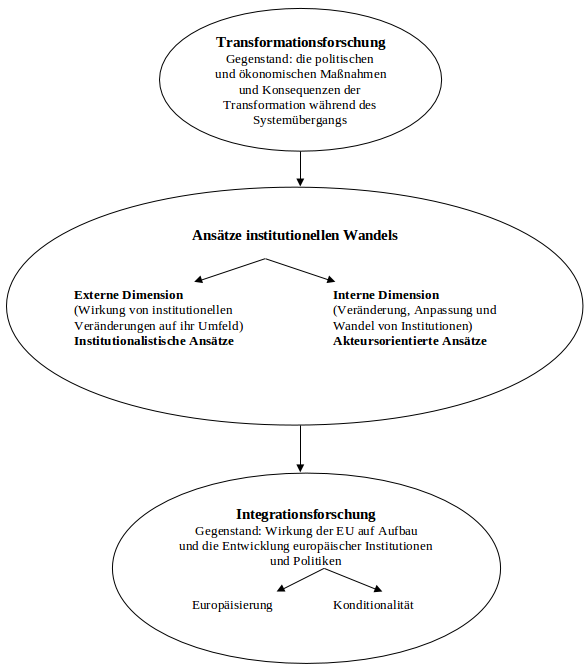
\includegraphics[width=5in]{Material/ForschungZuEuropUndKondi_ohneRand}\\

Quelle: in Anlehnung an \cite{huszak}: 75.
  \end{figure}
Erkennbar ist aus diesem Schema die Einbettung der Europäisierungs- und Konditionalitätsforschung in die übergeordneten theoretischen Konzepte Integrationsforschung, Forschung zu institutionellem Wandel und Transitionsforschung.\par
Moravcsik und Vachudova gehen von einer asymmetrischen Interdependenz zwischen Beitrittskandidat und der EU aus. Bei positiv verlaufender Konditionalität schätzen die Kandidatenländer die politischen Kosten der Anpassung ihrer nationalen Politiken niedriger ein als einen möglichen Ausschluss aus der EU und die damit verbundenen Nachteile (vgl. \cite{morvac}: 44).
\par
Schimmelfennig und Sedelmeier schlagen ein „external incentives“-Modell vor, das den Erfolg der EU-Konditionalität anhand von vier Faktoren beschreibt. Diese Faktoren führen dazu, dass nationale Regierungen EU-Regeln übernehmen, wenn die Vorteile größer sind als die Kosten der Anpassung. Die vier Faktoren sind “the determinancy of conditions, the size and speed of rewards, the credibility of threats and promises and size of adaption costs” (\cite{schsed05b}: 12). Angewandt auf die neuen EU-Mitgliedsländer kommen die Autoren zu dem Schluss, dass das „external incentives“-Modell von dem Typ der Konditionalität abhängt, wobei die Acquis-Konditionalität besser abschneidet als die politische Konditionalität (vgl. \cite{schsed05c}: 212). Die empirische Überprüfung führt zu dem Schluss, dass die Glaubwürdigkeit der Belohnung und die Höhe der politischen Anpassungskosten ausschlaggebend waren bei der Entscheidung der Anpassung an EU-Konzepte. Hinsichtlich der Glaubwürdigkeit erhöhte die Eröffnung von Verhandlungen die Wahrscheinlichkeit von nationalen Anpassungen, da sich damit in den Augen der Kandidatenländer der Wille der EU zeigte, die Verhandlungen auch zu einem Abschluss zu bringen (vgl. \cite{schsed05c}: 215). Weiterhin nimmt die Gefahr des Ausschlusses von der EU-Mitgliedschaft ab, je weiter der Assoziierungsprozess fortschreitet (vgl. \cite{dimit05}). Allerdings zeigte sich auch, dass hohe Anpassungskosten, die die Sicherheit oder Integrität des Staates oder das Überleben der Regierung gefährdeten, eine starke Behinderung darstellten, sogar bei glaubwürdigen Anreizen der EU. Nur im allerletzten Stadium der Verhandlungen („endgame“) haben die Staaten die Anpassungsleistungen vollzogen, sogar bei kurzfristigen hohen politischen Anpassungskosten im eigenen Land (\mbox{vgl. \cite{schetal}: 921}).\par

Huszka merkt in Bezug auf die Anwendung dieses „external incentives”-Modells auf den Balkan an: „However, while this ‘external incentive model’ according to which external rewards help elites to overcome domestic costs worked effectively in Central and Eastern Europe, its application to the Western Balkans is more problematic” (\cite{huszka}: 10). Hinzu kommt, dass die Mitgliedschaft für die in der vorliegenden Arbeit betrachteten Balkanstaaten noch stark in der Zukunft liegt. Daher sind die Belohnungen, die aktuell möglich sind, eher beschränkt.\par

Brusis konstatiert, dass demokratische Reformen verschiedene Ursachen haben und er geht davon aus, dass die Konditionalität der EU einen wesentlichen Einfluss hat, gibt aber auch zu bedenken: „Von der EU oder anderen externen Demokratisierungsakteuren gestellte Anforderungen sind aber weder a priori notwendige, noch hinreichende Bedingungen für innerstaatlichen Wandel“ (\cite{brusis05}: 298).

\subsection{Öffentliche Verwaltung und politische Konditionalität}

Die Notwendigkeit einer stabilen, effektiven und transparenten Verwaltung ist im Hinblick auf die Fähigkeit zur Übernahme des Acquis communautaire wichtig und wird in den Handreichungen der EU zur Übernahme des Acquis folgendermaßen formuliert: “A candidate country preparing for accession to the EU must bring its institutions, management capacity and administrative and judicial systems up to Union standards with a view to implementing the acquis effectively… At the general level, this requires a well-functioning and stable public administration built on an efficient and impartial civil service, and an independent and efficient judicial system” (\cite{eurcom05}: 7).\par
Die Existenz einer gut funktionierenden und stabilen öffentlichen Verwaltung ist eines der wesentlichen Kriterien innerhalb der EU-Konditionalität. Allerdings ist die öffentliche Verwaltung kein Kapitel des Acquis und unterliegt damit nicht der direkten Überprüfung anhand eines Kriterienkataloges. Die EU hat gemeinsame grundrechts- und allgemein rechtsstaatsbezogene Normen aufgestellt. Doch gibt es keine konkreten Vorgaben, wie demokratische Institutionen (Parlament, Regierung, Gerichte, Verwaltungsaufbau) organisiert sein sollen. Und in dieser Hinsicht existieren keine konkreten benchmarks, an denen sich die Beitrittsländer orientieren und deren Erfüllung man untersuchen könnte (vgl. \cite{brusis09}: 196). Von der EU wird das Thema Verwaltungsreform unter „politische Bedingungen“ behandelt und diese „politischen Kriterien“ nehmen einen festen Raum ein in den jährlichen Fortschrittsberichten der EU zu den Beitrittskandidaten.\par
Die Konditionalitätsforschung geht also von einem starken Zugzwang aus, in den die Kandidatenländer geraten, der dazu führt, dass sie die Anforderungen der EU zum Umbau ihrer nationalen Strukturen erfüllen. Dies wird deutlich im Rahmen der geforderten Übernahme des Acquis mit konkreten Kapiteln, die im nationalen Rahmen umzusetzen sind. Im Zusammenhang mit der Verwaltungsmodernisierung ist dies nicht so eindeutig nachvollziehbar, da es sich nicht um ein Kapitel des Erweiterungsacquis handelt.\par
Kennzeichnend für die Konditionalitätsforschung ist also die Konzentration auf die Frage, was die Veränderungen insbesondere in den Beitrittskandidaten befördert. Zentraler Gesichtspunkt sind dabei die Bedingungen der EU, die einem Beitritt vorausgehen, d.h. die Konditionalität. Im Kontext der vorliegenden Arbeit geht es hierbei insbesondere um die politische Konditionalität, unter die das Thema Verwaltungsmodernisierung fällt, ist kein Kapitel des Acquis und entfaltet daher vergleichsweise geringere Konditionalität. Dennoch wird die Struktur der Verwaltung und ihre Modernisierung bei den politischen Kriterien abgehandelt, wie z.B. in den jährlichen Fortschrittsberichten deutlich wird.\par
Insofern ist die Konditionalitätsforschung auch auf das Thema Verwaltungsmodernisierung in den Beitrittsländern anwendbar und kann wertvolle Hinweise liefern. \par
Im nächsten Abschnitt der Untersuchung werden deshalb die praktischen Aspekte der EU-Erweiterung, jeweils mit Rückbindung an das Thema Verwaltungsentwicklung und Verwaltungsmodernisierung, überblicksartig dargestellt. Es wird im weiteren Verlauf der Arbeit zu prüfen sein, welchen Stellenwert Verwaltungsmodernisierung für die EU im Zuge der Erweiterungsstrategie hat und wie Verwaltungsmodernisierung in der Erweiterungspolitik vorkommt.

%\chapter{Grundlagen der EU-Erweiterung }
Ob und in welchem Umfang die EU erweitert werden soll, ist eine politische Entscheidung. Auch die zeitlichen Abläufe für den Beitritt von Staaten zur EU werden durch politische Entscheidungen dominiert, wenngleich für diesen Aspekt binnenorganisatorische Abläufe informell ebenfalls von Bedeutung sein könnten. Die Gestaltung eines Beitrittsprozesses wirft viele Fragen auf, die teils fallspezifisch, teils allgemeiner Art sind. In Betracht kommen politische, ökonomische, soziale und administrative Probleme des gewünschten oder notwendigen Wandels. \par
Prozesse des Wandels sind sowohl Gegenstand verschiedener theoretischer Überlegungen als auch eine Gelegenheit, entsprechende Praxiserfahrungen zu sammeln. Da die EU seit ihrer Gründung bereits mehrfach erweitert wurde, liegt schon ein umfangreiches Praxiswissen zu Beitrittsprozessen zur EU vor; von diesem ist allerdings nicht genau bekannt, in welchem Umfang es fallspezifisch oder wieweit es übertragbar ist.
\section{Die Erweiterung der EU in der Praxis }
Die Europäische Union in den 1950er Jahren, zunächst mit der Gründung der Europäischen Gemeinschaften, umfasste sechs Staaten (Belgien, Frankreich, Deutschland, Luxemburg, Italien und die Niederlande). Ziel war es, nach dem Zweiten Weltkrieg einen wirtschaftlichen Staatenverbund zu schaffen, der die Gefahr gewaltsamer Auseinandersetzungen vermindern und durch einen gemeinsamen Markt die Wirtschaft ankurbeln sollte. Der EU, mit den Römischen Verträgen von 1957 gegründet, gehören inzwischen 27 Länder an, die in sogenannten Erweiterungsrunden aufgenommen wurden. Länder, die geografisch zu Europa gehören und demokratisch verfasst sind, können in die EU aufgenommen werden. Die umfassendste Erweiterung wurde 2004 umgesetzt mit der Aufnahme von Zypern, der Tschechischen Republik, Estland, Ungarn, Lettland, Malta, Polen, der Slowakei und Sloweniens. In derselben Erweiterungsrunde, aber mit einer Verzögerung, traten Bulgarien und Rumänien 2007 der EU bei. Die Aufnahme Kroatiens ist für 2013 vorgesehen.\par
\renewcommand{\arraystretch}{1.5}
\begin{table}[!hbt]\vspace{1ex}
\centering
\footnotesize
\caption{Geschichte der Verträge zur Europäischen Gemeinschaft}

\begin{tabular}{|Q{12mm}|Q{12mm}|Q{4cm}|Q{7cm}|}\hline
Unter\-zeichnet &In Kraft & Name&Inhalt\\\hline
1951&1952&Vertrag von Paris&Europäische Gemeinschaft für Kohle und Stahl (EGKS)\\\hline
1957&1958&Verträge von Rom&EWG-Vertrag, Europäische Wirtschaftsgemeinschaft (EWG) und der EURATOM-Vertrag\\\hline
1965&1967&Fusionsvertrag&Einsetzung eines gemeinsamen Rates und einer gemeinsamen Kommission der Europäischen Gemeinschaften\\\hline
1986&1987&Einheitliche Europäische Akte&Binnenmarkt eingeführt\\\hline
1992&1993&Vertrag von Maastricht&Europäische Union\\\hline
1997&1999&Vertrag von Amsterdam&Änderungen des Maastrichter Vertrages\\\hline
2001&2003&Vertrag von Nizza&Änderungen der Verträge von Rom und Amsterdam\\\hline
2004& &Verfassungsvertrag&Verfassung für Europa (abgelehnt)\\\hline
2007&2009&Vertrag von Lissabon&Änderungen des Vertrages über die Europäische Union (EUV) und des Vertrages über die Arbeitsweise der Europäischen Union (AEUV)\\\hline
\multicolumn{4}{c}{}
\end{tabular}\\
{\normalsize Quelle: nach \cite{moller}: 4 (eigene Ergänzung zu Vertrag von Lissabon).}
\end{table}
\renewcommand{\arraystretch}{1.2}
\subsection{Das Verfahren zur Aufnahme eines Staates }
Die Aufnahme neuer Mitglieder war von Anfang an in der Gründungsidee der EU enthalten. In Art. 6 Absatz 1 des Vertrages über die Europäische Union (EUV) ist festgelegt: „Die Union beruht auf den Grundsätzen der Freiheit, Demokratie, der Achtung der Menschenrechte und Grundfreiheiten sowie der Rechtsstaatlichkeit; diese Grundsätze sind allen Mitgliedstaaten gemeinsam“. Artikel 49 des Vertrages legt fest: „Jeder europäische Staat, der die in Art. 6 Abs. 1 genannten Grundsätze achtet, kann beantragen, Mitglied der Union zu werden“. Über diese allgemeine Verfügung hinaus muss die EU in der Lage sein, neue Mitglieder aufzunehmen, was im Einzelfall entschieden wird. Eine Aufnahme geschieht durch Konsensbeschluss der EU-Mitgliedstaaten mittels ihrer Vertreter im Ministerrat oder Europäischen Rat. Nach dem Antrag auf Aufnahme wird aufgrund einer Stellungnahme der Europäischen Kommission entschieden, ob das Land als Beitrittskandidat anerkannt wird. Innerhalb der Kommission ist die Generaldirektion Erweiterung zuständig für Koordination, regelmäßige Berichterstattung sowie enge Zusammenarbeit mit den Line DGs und den Arbeitsgruppen des Europäischen Rates (vgl. \cite{summa}: 13). Der Delegation der EU in den Kandidatenländern kommt ebenfalls eine wichtige Rolle zu in der Koordination zwischen der Europäischen Kommission in Brüssel und den Kandidatenländern.\par
Vor der Aufnahme in die EU findet ein Prozess der Verhandlungen statt zu unterschiedlichen Politikbereichen, um die Übernahme des vollständigen gemeinschaftlichen Besitzstandes zu gewährleisten. Dies ist eine Aufnahmebedingung. Vor einer Aufnahme muss dann der entsprechende Vertrag in den Mitgliedstaaten nach dem dafür vorgesehenen Verfahren ratifiziert werden. Schließlich muss noch das Europäische Parlament seine Zustimmung geben (vgl. \cite{euko07}: 6f).
\par
In den Kandidatenländern wird die Arbeit im Zusammenhang mit dem Beitrittsprozess meist von einem Minister in einem bestehenden Ministerium oder aus einem eigens geschaffenen Ministerium für den Erweiterungsprozess koordiniert (vgl. \cite{summa}: 14).\par
Die Stadien im Erweiterungsprozess sind im folgenden Schema überblicksartig dargestellt:
\begin{figure}[H]
  \centering

   \caption{Phasenmodell des EU-Beitritts }
  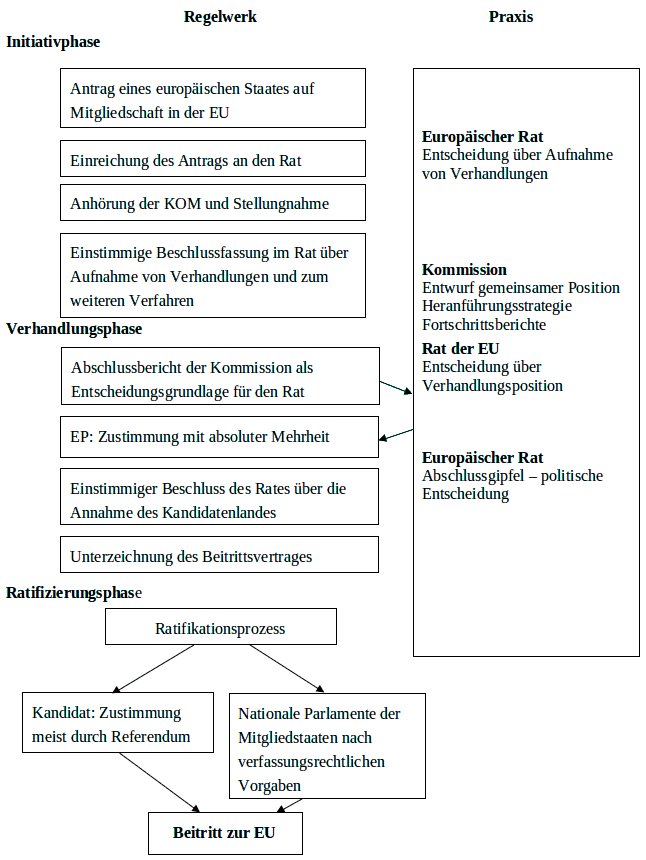
\includegraphics[width=5in]{Material/Phasenmodell_ohneRand}\\

Quelle: in Anlehnung an \cite{wessels}: 449.
\end{figure}
In der Darstellung ist der gesamte Prozess der Aufnahme in den einzelnen erforderlichen Schritten schematisch dargestellt. Dabei werden drei Hauptphasen unterschieden: Die Initiativ-, die Verhandlungs- und die Ratifizierungsphase. Der angestrebte EU-Beitritt der drei Untersuchungsländer ist aktuell geprägt von der Umsetzung und Abarbeitung der Heranführungsstrategie und der jährlichen Berichterstattung (im Schema Fortschrittsberichte genannt).\par

Nachdem ein Land offiziell den Aufnahmeantrag gestellt hat, bekommt es von der EU-Kommission einen Fragebogen zu allen Bereichen des Acquis communautaire übersandt. Diese Fragebögen zu den bestehenden Institutionen, policies und Infrastruktur müssen von dem Antragsteller ausgefüllt und der EU-Kommission übersandt werden. Auf der Grundlage dieser Antworten erarbeitet die Kommission eine vorläufige Stellungnahme zu dem Beitrittsgesuch des Landes, mit einer Empfehlung, ob und ggf. wann das Land die Beitrittsverhandlungen beginnen kann. Um offiziell Beitrittskandidat zu werden, muss der Europäische Rat/Council of Ministers formal beschließen, mit dem Land Beitrittsverhandlungen aufzunehmen. Die Kommission tritt dann in einen Prozess des “screening” ein, in dem die Gesetzgebung und policies des Landes mit der EU verglichen werden, “in order to make longterm plans to bring applicant countries up to EU standards“ (\cite{grab10}: 3).
Die praktische Durchführung der Erweiterung ist ein komplexer Prozess, der sich evolutionär entwickelt hat. Keine Erweiterungsrunde war bisher mit der vorherigen identisch und in jedem Fall wurden neue Erweiterungsinstrumente eingeführt oder bestehende weiterentwickelt (vgl. \cite{kochenov}: 16). Die bisherigen Aufnahmen mit den Schritten vom Beitrittsantrag bis zum Beitritt sind im folgenden Schema mit der in der Literatur vorherrschenden Bezeichnung der jeweiligen Erweiterung dargestellt.\\
\begin{table}[H]\vspace{1ex}\centering
\caption{Bisherige EU-Erweiterungen}
\footnotesize
\begin{tabular}{|p{2cm}|p{2cm}|p{2cm}|p{2cm}|p{2cm}|p{2cm}|}\hline
&Beitritts\-antrag&Stellung\-nahme Kommis\-sion&Beginn Beitritts\-verhand\-lungen&Unter\-zeichnung Beitritts\-vertrag&Beitritts\-datum\\\hline
\multicolumn{6}{|p{12cm}|}{1. Norderweiterung} \\\hline 
Vereinigtes Königreich&
10.05.1967 (09.08.61)*&
19.09.1967&
30.06.1970&
22.01.1972&
01.01.1973\\\hline
Dänemark&
11.05.1967 (10.08.61)*&
19.09.1967&
30.06.1970&
22.01.1972&
01.01.1973\\\hline
Irland&
11.05.1967 (10.08.61)*&
19.09.1967&
30.06.1970&
22.01.1972&
01.01.1973\\\hline
\multicolumn{6}{|p{12cm}|}{2. Süderweiterung}\\\hline
Griechenland &
12.06.1975&
29.01.1976&
27.07.1976&
28.05.1979&
01.01.1981\\\hline
Portugal&
28.03.1977&
19.05.1978&
17.10.1978&
12.06.1985&
01.01.1986\\\hline
Spanien&
28.07.1977&
29.11.1978&
05.02.1979&
12.06.1985&
01.01.1986\\\hline
\multicolumn{6}{|p{12cm}|}{3. EFTA-Erweiterung}\\\hline
Österreich&
17.07.1989&
01.08.1991&
01.02.1993&
24.04.1994&
01.01.1995\\\hline
Schweden&
01.07.1991&
31.07.1992&
01.02.1993&
24.04.1994&
01.01.1995\\\hline
Finnland&
18.03.1992&
04.11.1992&
01.02.1993&
24.04.1994&
01.01.1995\\\hline
\multicolumn{6}{|p{12cm}|}{4. Erweiterung Mittel- und Osteuropa}\\\hline
Ungarn&
31.03.1994&
16.07.1997&
31.03.1998&
16.04.2003&
01.05.2004\\\hline
Polen&
05.04.1994&
16.07.1997&
31.03.1998&
16.04.2003&
01.05.2004\\\hline
Slowakei&
27.06.1995&
16.07.1997&
15.02.2000&
16.04.2003&
01.05.2004\\\hline
Lettland&
13.10.1995&
16.07.1997&
15.02.2000&
16.04.2003&
01.05.2004\\\hline
Estland&
24.11.1995&
16.07.1997&
31.03.1998&
16.04.2003&
01.05.2004\\\hline
Litauen&
08.12.1995&
16.07.1997&
15.02.2000&
16.04.2003&
01.05.2004\\\hline
Tschechien&
17.01.1996&
16.07.1997&
31.03.1998&
16.04.2003&
01.05.2004\\\hline
Slowenien&
10.06.1996&
16.07.1997&
31.03.1998&
16.04.2003&
01.05.2004\\\hline
Rumänien&
22.06.1995&
16.07.1997&
15.02.2000&
25.04.2005&
01.01.2007\\\hline
Bulgarien&
14.12.1995&
16.07.1997&
15.02.2000&
25.04.2005&
01.01.2007\\\hline
\multicolumn{6}{|p{12cm}|}{* In Klammern der Zeitpunkt des jeweils ersten Beitrittsantrages: In Folge des Scheiterns der Verhandlungen mit dem Vereinigten Königreich kam es ebenfalls zum Abbruch der Verhandlungen mit den übrigen Bewerbern.}\\\hline
\multicolumn{6}{c}{}
\end{tabular}\\
Quelle: \cite{wessels}: 451.
\end{table}
Aus dieser Darstellung wird ersichtlich, dass die bisherigen EU-Erweiterungen in Wellen stattgefunden haben, mit der Aufnahme von Ländern oft in Gruppen. Darauf sind auch die umgangssprachlichen Benennungen wie „EU-Süderweiterung“ oder „EU-Osterweiterung“ zurückzuführen. 

\subsection{EU-Erweiterungen in der Wahrnehmung der Öffentlichkeit}
Die Wahrnehmung der Öffentlichkeit in EU-Ländern hinsichtlich einer erneuten EU"=Erweiterung lässt deutliche Unterschiede erkennen. Dabei wird in den „neuen“ EU-Ländern eine erneute Erweiterung am positivsten gesehen und in den „alten“ EU-15 Ländern am negativsten. Weiterhin sinkt im Durchschnitt die Befürwortung einer Erweiterung um ca. 3 Prozentpunkte jährlich. In Polen wird die Erweiterung am positivsten bewertet, mit 74\% im Jahre 2008. Die Befürwortung einer erneuten Erweiterung lag im EU-Durchschnitt im selben Jahr nur bei 47\% (EU-27). In Ländern mit geringer Begeisterung der Bevölkerung für eine erneute Erweiterung, wie Österreich, Frankreich und Deutschland, stehen die Regierungen einer Südosterweiterung positiv gegenüber, ungeachtet der Einstellung der Mehrheit der Bevölkerung (vgl. \cite{mus}: 20).\par

In den Beitrittsländern, die Gegenstand der vorliegenden Arbeit sind, hat sich die Unterstützung der Bevölkerung für den EU-Beitritt unterschiedlich entwickelt. So ist in Montenegro die Zustimmung zur EU-Orientierung des Landes im Zeitraum 2009-2010 von 67\% auf 73\% gestiegen. In Mazedonien dagegen fiel die Zustimmung zu einem EU-Beitritt des Landes im selben Zeitraum von 62\% auf 60\%. Im gesamten Westlichen Balkan ist die EU-Orientierung der Bevölkerung in Albanien im Jahr 2010 mit 81\% am höchsten, hat aber dennoch 9 Prozentpunkte Zustimmung gegenüber dem Vorjahr verloren (vgl. \cite{gallup10}).\par
In einer repräsentativen Umfrage in den Mitgliedsländern der EU wird deutlich, dass die Bevölkerung dort im Zusammenhang mit einer erneuten Erweiterung vor allem Freiheit und demokratische Werte, noch vor ökonomischen Überlegungen, in Bezug auf Europa als Ganzes wichtig findet. In Bezug auf das eigene Land war den Befragten allerdings der ökonomische Aspekt der Erweiterung wichtiger, wie aus folgender Tabelle ersichtlich:
\begin{figure}[H]\centering
\setlength\belowcaptionskip{10pt}
  \caption{Umfrage zur EU-Erweiterung in den Mitgliedstaaten der EU }
  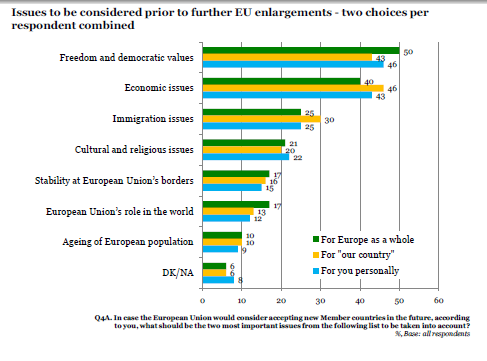
\includegraphics[width=5in]{Material/Umfrage}
\end{figure}
\vspace{-1cm}
{\centering Quelle: Eurobarometer 2009: 20.\footnote{Das Eurobarometer ist eine in regelmäßigen Abständen von der Europäischen Kommission in Auftrag gegebene öffentliche Meinungsumfrage in den Ländern der EU. Dabei werden jeweils immer die gleichen Standardfragen als auch wechselnde Fragen zu unterschiedlichen Themen gestellt.}
  \par
}

In den Mitgliedstaaten der EU wurde folgende Frage gestellt: Falls Die EU in der Zukunft über die Aufnahme neuer Mitglieder entscheiden würde, welche zwei Themen (von der vorgegebenen Liste) sollten dabei berücksichtig werden?

\subsection{Politische Konditionalität im Aufnahmeverfahren}
Um Mitgliedstaat zu werden, muss ein Land den kompletten gemeinschaftlichen Besitzstand der Union (Acquis communautaire) akzeptieren, d.h. in nationales Recht übernehmen. Das gesamte Recht der Europäischen Gemeinschaften und der Europäischen Union wird unter dem Begriff „gemeinschaftlicher Besitzstand“ zusammengefasst. Es handelt sich um rund 15.000 Rechtsakte auf nahezu 100.000 Druckseiten (Stand 2008). Der Acquis communautaire, der seit 1973 in 31 thematische Kapitel eingeteilt war, wurde nach Abschluss der letzten Erweiterungswelle in 35 Kapiteln reorganisiert (vgl. \cite{summa}: 14). \par

\begin{table}[H]
\centering
\setlength\belowcaptionskip{10pt}
\caption{Die Kapitel des Acquis communautaire:}
\begin{tabular}{|c p{7cm}|c p{7cm}|}\hline
1:&Freier Warenverkehr&19:&Beschäftigung und Soziales\\
2:&Freizügigkeit für Arbeitnehmer&20:&Unternehmen und Industrie\\
3:&Niederlassungsrecht und freier Dienstleistungsverkehr&21:&Transeuropäische Netze\\
4:&Freier Kapitalverkehr&22:&Regionalpolitik und Koordinierung der strukturellen Instrumente\\
5:&Öffentliches Auftragswesen&23:&Judikative und Grundrechte\\
6:&Gesellschaftsrecht&24:&Justiz, Freiheit und Sicherheit\\
7:&Rechte am geistigen Eigentum&25:&Wissenschaft und Forschung\\
8:&Wettbewerb&26:&Bildung und Kultur\\
9:&Finanzdienstleistungen&27:&Umwelt\\
10:&Informationsgesellschaft und Medien&28:&Verbraucher- und Gesundheitsschutz\\
11:&Landwirtschaft und ländliche Entwicklung&29:&Zollunion\\
12:&Lebensmittelsicherheit, Tier- und Pflanzenschutzpolitik&30:&Außenbeziehungen\\
13:& Fischerei&31:&Außen-, Sicherheits- und Verteidigungspolitik\\
14:&Verkehr&32:&Finanzkontrolle\\
15:&Energie&33:&Finanz- und Haushaltsvorschriften\\
16:&Steuern&34:&Institutionen\\
17:&Wirtschaft und Währung&35:&Sonstiges \\
18:&Statistik&&\\\hline
\multicolumn{4}{c}{}
\end{tabular}
http://www.europarl.europa.eu/brussels/website/media/modul\_01/Zusatzthemen\\/Pdf/Acquis.pdf  (Aufgerufen: 10.9.2012).
\end{table}
Obwohl es während der Süderweiterung keine auf bestimmte Länder abgestimmten Bedingungskataloge und kein regelmäßiges Monitoring gab, war neben der Übernahme des Acquis communautaire die Demokratie als Staatsmodell ein Aufnahmekriterium (vgl. \cite{pridham07}: 451). Die Assoziierungsvereinbarung mit Griechenland wurde nach dem Staatsstreich der Generäle 1967 eingefroren und der ursprüngliche Aufnahmeantrag Spaniens blieb zunächst unbeantwortet. Dies zeigt, dass die demokratische Verfasstheit schon in dieser Zeit der EU-Erweiterung ein, wenn auch implizites Kriterium war. In der Folge ist die EU von der reinen Annahme des Acquis communautaire als Beitrittsbedingung zu weiter gefassten Reform- und Transformationszielen mit zusätzlichen Voraussetzungen übergegangen (vgl. \cite{dimit04}: 8-9).\par
Eine Art politischer Konditionalität wurde erstmals Mitte der 1990er Jahre eingeführt mit den Europe Agreements, die ausgesetzt werden konnten. Gefordert wurde Rechtsstaatlichkeit, Achtung der Menschenrechte, ein Mehrparteiensystem und freie Wahlen (Grabbe zit. in \cite{pridham07}).\par
Seit der Eröffnung einer Beitrittsperspektive für die ehemals kommunistischen Staaten Mittel- und Osteuropas wurden die Kriterien für einen potenziellen Beitritt mit den sogenannten Kopenhagen-Kriterien von 1993 konkreter benannt. Neben ökonomischen Voraussetzungen wird institutionelle Stabilität als eine notwendige Bedingung und Grundlage für demokratische und rechtsstaatliche Ordnung gefordert (vgl. \cite{kreile}: 654). So legte der Rat fest:\par

„Als Voraussetzung für die Mitgliedschaft muss der Beitrittskandidat eine institutionelle Stabilität als Garantie für demokratische und rechtsstaatliche Ordnung, für die Wahrung der Menschenrechte, sowie die Achtung und den Schutz von Minderheiten verwirklicht haben; sie erfordert ferner eine funktionsfähige Marktwirtschaft sowie die Fähigkeit, dem Wettbewerbsdruck und den Marktkräften innerhalb der Union standzuhalten.“ \footnote{Europäischer Rat Kopenhagen, Schlussfolgerungen des Vorsitzes, 21. bis 23. Juni 1993, http://www.consilium.europa.eu/ueDocs/cms\_Data/docs/pressData/de/ec/72924.pdf, S.13 (Aufgerufen: 21.9.2012).}\par

Um die Kriterien von Kopenhagen in konkrete Maßnahmen zu überführen, wurde 1994 das Instrument der „pre-accession strategy“ eingeführt (vgl. \cite{lipsch}). \par

Damit waren die Erweiterungsbedingungen für die Zukunft fixiert. Die EU-Institutionen überprüfen regelmäßig, ob die (potenziellen) Beitrittskandidaten dieses sogenannte politische Kriterium erfüllen. In jährlichen Berichten, die Fortschrittsberichte genannt werden und 1998 erstmals von der Kommission erstellt wurden, überprüft diese, ob Legislative, Exekutive und Verwaltung sowie das Gerichtswesen in den beitrittswilligen Ländern verfassungskonform arbeiten, ob Minderheitenrechte und individuelle Grundrechte geschützt werden und Korruption bekämpft wird (vgl. \cite{brusis09}: 195).
\par
Seitdem kommt der mit den Kopenhagen-Kriterien verbundenen politischen Konditionalität im Rahmen der EU-Erweiterung besondere Bedeutung zu. Ein Wertekatalog gekoppelt an finanzielle Unterstützung im Beitrittsprozess ist das Kennzeichen dieser Entwicklung. Kneuer bezeichnet die Konditionalität des Erweiterungsprozesses als Anreiz-Druck-System, das den attraktiven Anreiz der Mitgliedschaft bereithält, aber ebenso Druck zu allgemeiner Demokratisierung aufrechterhält und bei demokratischen Defiziten oder Fehlentwicklungen den Druck mit Negativmaßnahmen verstärken kann (vgl. \cite{kneuer07}: 108).\par
Weitere Kriterien bezogen auf die Beitrittsverhandlungen wurden in Madrid anlässlich der Tagung des Europäischen Rates am 14./15. Dezember 1995 formuliert, unter anderem die Forderung nach Verwaltungsreformen in den Kandidatenländern (vgl. \cite{dimit02}). Bezogen auf die Heranführungsstrategie für die Länder Mittel- und Osteuropas forderte der Europäische Rat:
„diese Strategie muß intensiviert werden, um die Voraussetzungen für eine schrittweise und harmonische Integration dieser Länder zu schaffen, und zwar insbesondere durch die Entwicklung der Marktwirtschaft, die Anpassung der Verwaltungsstrukturen dieser Länder und die Schaffung stabiler wirtschaftlicher und monetärer Rahmenbedingungen“ (\cite{eurrat}).\par
Damit haben die Mitgliedsländer Elemente von „Good Governance“ eingeführt, mit expliziter Erwähnung der Anpassung von Verwaltungsstrukturen (vgl. \cite{sabzei}: 307).\par
Rechtliche und administrative Kapazitäten mussten nun vorhanden sein und wurden als Voraussetzung der Umsetzung des Acquis communautaire gesehen. Damit war die politische Konditionalität als neues Instrument des EU-Erweiterungsprozesses in der letzten Dekade des 20. Jh.s eingeführt worden (vgl. \cite{tomtul}: 380).\par
Die zusätzlichen Bedingungen beziehen sich zum Teil auf Bereiche, in denen die EU selbst nicht über Normenkompetenz oder einheitliche Regelungen verfügt. Zwar gibt es keine direkte Sanktionsmöglichkeit bei der Nichterfüllung der entsprechenden Kriterien, z.B. durch finanzielle Sanktionen. Dennoch ist die „politische Konditionalität“ ein wesentliches, neues Element im EU-Erweiterungsprozess. Die Zunahme der Bedeutung von institution building bzw. staatlicher Kapazitäten innerhalb der Erweiterungspolitik der EU wird von Sabel und Zeitlin sogar als Paradigmenwechsel bezeichnet, der sich graduell innerhalb der 1990er Jahre vollzog (vgl. \cite{sabzei}: 307).\par
Der Stellenwert und der Umgang mit der Reform der öffentlichen Verwaltung seitens der EU im Erweiterungsprozess wird im folgenden Kapitel dargestellt.

\subsection{Kompetenz der EU bezüglich der Verwaltung}
\label{subsec:Kompetenz der EU}
Im Bereich öffentliche Verwaltung hat die EU keine Regelungskompetenz in den Mitgliedstaaten und keinen direkten Einfluss auf das administrative System ihrer Mitglieder. Alle Mitgliedsländer können die institutionellen Arrangements ihrer öffentlichen Verwaltungen frei wählen, einschließlich des Systems der Ausführung von Staatsaufgaben. Die EU ist bei der Umsetzung des Gemeinschaftsrechts auf die nationalen Verwaltungen angewiesen, ohne Organisationsstrukturen oder Personalstrukturen direkt beeinflussen zu können. Weiterhin gibt es innerhalb der EU keine „Blaupause“, die nationale öffentliche Verwaltungen übernehmen können. Es gibt nicht einmal eine Vorstellung eindeutiger „Best Practice“-Beispiele in Bezug auf Strukturen und Verfahrensweisen, obwohl das „White Paper on European Governance“ von 2001 Ausführungsstandards zu beschreiben versucht. „The lack of a clear overarching public administration model and the relatively weak European powers for the imposition of specific changes in domestic administrations might also be considered as a factor for slowing down European Integration“ (\cite{sverdrup}: 44).\par

Das Dilemma der EU hinsichtlich der öffentlichen Verwaltung in den Beitrittskandidaten wird in einem Evaluierungsbericht zur Institutionenentwicklung für die osteuropäischen Beitrittskandidaten deutlich: “Although there are, in many sectors, highly detailed acquis requirements as to what the public administration should deliver, and to what standards, there is of course no acquis on public administration per se” (\cite{omas}: 3). Die Evaluatoren konstatieren, dass die öffentliche Verwaltung nicht Teil des Acquis ist und seitens der EU auch keine Vorgaben für Reformprojekte zur öffentlichen Verwaltung gemacht wurden: “There is no acquis on public administration and there is no evidence that any coordinated attempt has been made by the Commission Services to orientate the PHARE national Public Administration Reform Programmes in any defined direction.” (\cite{omas}: 1). \par

Die Europäische Union hat anlässlich der Erweiterungen 1973, 1980, 1986 und 1995 keine Begutachtung der administrativen Kompetenzen der Aufnahmeländer durchgeführt (vgl. \cite{ziller}: 138). Dennoch sind seit 1997 administrative Fragen im Zusammenhang mit der EU-Erweiterung zunehmend in den Vordergrund gerückt. „Candidate countries have been put under pressure to modernize their administrations, that is, to develop a professional civil service and build institutional capacity to implement and enforce legal norms” (\cite{olsen}). So hat die Präsidentschaft des Europäischen Rates nach ihrem Treffen in Kaeken am 14. und 15. Dezember 2001 angemahnt, dass die Kandidatenländer ihre Anstrengungen fortsetzen müssen, insbesondere um ihre administrativen Kapazitäten auf das geforderte Niveau zu bringen (vgl. \cite{olsen}). Hintergrund dieser Forderung ist vor allem die Notwendigkeit, nationale Verwaltungsstrukturen zu entwickeln, die für die Interaktion mit der EU verantwortlich sind für die Verhandlungen mit Brüssel und die Umsetzung des Acquis.

\subsection{Das Konzept Europäischer Verwaltungsraum}
\label{subsec:Verwaltungsraum}
Nachdem nun deutlich wurde, dass es keinen konkreten Acquis zur Ausgestaltung der öffentlichen Verwaltung gibt, stellt sich die Frage, ob es möglicherweise durch die Zunahme supranational zustande gekommener Entscheidungsprozesse zu einer Europäisierung im Verwaltungshandeln kommt. Einerseits hat die EU keinen direkten Einfluss auf die verwaltungsmäßige Umsetzung von Gemeinschaftsrecht. Andererseits erscheint eine Art Blaupause für Strukturen einer europäisch orientierten Verwaltung sinnvoll angesichts der möglichen Aufnahme von Ländern mit schwacher demokratischer Staatstradition (z.B. Bosnien-Herzegowina, Albanien). Vor allem die Organisation für Ökonomische Zusammenarbeit und Entwicklung (OECD) mit ihrem SIGMA-Programm (Support for Improvement in Governance and Management) war seit 1998 maßgeblich an der Entwicklung eines Konzeptes zu einem europäischen Verwaltungsraum (European Administrative Space) beteiligt. SIGMA kam im Rahmen einer Studie zu der Auffassung, dass die strikte Auslegung von Artikel 39 Absatz 4 EG-Vertrag und die strikte Auslegung des Begriffs der „Öffentlichen Verwaltung“ durch den EuGH zur Schaffung eines Verwaltungsraumes in den Mitgliedstaaten führen wird. Die European Group of Public Administration (EGPA) des Internationalen Instituts für Verwaltungswissenschaften richtete 2002 eine Tagung aus zum Thema: „ The European Administrative Space: Governance in Diversity“ (\cite{mangenot}: 13).\par
In Anbetracht der unterschiedlichen Traditionen der öffentlichen Verwaltung in Europa gibt es Stimmen, die vor der Ausrufung eines gemeinsamen europäischen Rahmens für den öffentlichen Sektor warnen (vgl. \cite{olsen}). Gründe für diese angemahnte Vorsicht sind unter anderem nach wie vor nationale Weichenstellungen. Die EU hat gerade erst angefangen, die Reform der öffentlichen Verwaltung als eigenständiges Politikfeld zu sehen (vgl. \cite{schmar}). Weiterhin hat die EU kein starkes Rollenmodell im Bereich Public Management für die Mitgliedstaaten geschaffen und die zentrale Verwaltung der EU erscheint als ein Patchwork einzelner unterschiedlicher nationaler Traditionen. Dennoch kann von einem Trend hin zu einem spezifischen europäischen Ansatz im Bereich öffentlicher Verwaltung ausgegangen werden. Dies kann auch damit erklärt werden, dass es in den EU-Mitgliedsländern eine gemeinsame Idee von Staat, Souveränität und Demokratie gibt, zumindest im Vergleich mit anderen Kontinenten. Insbesondere der ‘acquis communautaire’, der zentrale Teil der EU-Gesetzgebung, stellt eine Basis dar für gemeinsame administrative Standards und Regeln, die Eingang finden in das System der nationalen öffentlichen Verwaltung (vgl. \cite{raarut}: 31). Weiterhin entspricht das Konzept eines Europäischen Verwaltungsraumes der Forderung von Wirtschaftsakteuren nach einheitlichen Wettbewerbsbedingungen und nach administrativer Kooperation über Ländergrenzen hinweg (vgl. \cite{bogjan}: 245). \par
Gemeinsame Grundwerte und -prinzipien der europäischen öffentlichen Verwaltung haben zunehmend zu Konvergenz zwischen nationalen Verwaltungen geführt. „The European Administrative Space (EAS) represents an evolving process of increasing convergence between national administrative legal orders and administrative practices of member states. The EAS concerns basic institutional arrangements, processes, common administrative standards, civil service values and administrative culture. It is difficult to speak of a European model of Public Administration, but the EAS, albeit a metaphor, signifies a convergence and states the basic values of public administration as a practice and profession in Europe” (\cite{oecd99}: 15). \par
Mit der Stärkung und Erweiterung der EU sind im Hinblick auf die administrative Konvergenz viele Hoffnungen verbunden. So wird von einer Homogenisierung der administrativen Kapazitäten ausgegangen, unter Einbezug nationaler und kultureller Besonderheiten. Dabei geht es nicht um eine „Gleichschaltung“ der administrativen Systeme, sondern um eine Angleichung der Serviceerbringung hinsichtlich Qualität und Effizienz im Sinne eines Public Service Standards, so eine Sichtweise (vgl. \cite{dorta}: 8f.). Allerdings gibt es auch Stimmen, die auf die Bedeutung der nationalen Verwaltungstraditionen hinweisen. Selbst eindeutig auf europäischen Regelungen basierende Veränderungsprozesse der nationalen Verwaltungen sind nach dieser Sichtweise entscheidend durch den nationalen Kontext geprägt (vgl. \cite{herit}).\par
Auf einer praktischen Ebene kann man bei dem ‚European Public Administration Network' (EUPAN)\footnote{http://www.eupan.eu/en/content/show/\&tid=188 (Aufgerufen 15.10.2012).}, in dem Minister und Generaldirektoren des öffentlichen Dienstes vertreten sind, von einer Europäisierung durch Verwaltungskooperation sprechen. In dem Netzwerk war von Anfang an auch die Europäische Kommission vertreten mit dem für die Verwaltungsreform zuständigen Kommissar der Generaldirektion Verwaltung und Personal (ADMIN); dennoch steht EUPAN außerhalb des förmlichen Rahmens der Gemeinschaft. EUPAN dient als Netzwerk und fördert durch das Zusammentreffen von nationalen Beamten den Austausch über Ländergrenzen hinweg (vgl. \cite{mangenot}: 49).\par
Eine andere (europäische) Initiative, das ‚Common Assessment Framework’ (CAF) mit dem Ziel, Exzellenz in der europäischen öffentlichen Verwaltung zu fördern, soll hier ebenfalls erwähnt werden. Das CAF wurde im Anschluss an das Ministertreffen vom November 1998 entwickelt, als die Schaffung eines „Europäischen Qualitätspreises“ auf Grundlage von Leistungsindikatoren vorgeschlagen wurde. Das im Mai 2000 in Lissabon auf der ersten europäischen Qualitätskonferenz vorgestellte CAF basiert auf Modellen der Europäischen Stiftung für Qualitätsmanagement (European Foundation for Quality Management) und ist ein Instrument der Selbstbewertung von öffentlichen Verwaltungen (vgl. \cite{mangenot}: 52).\par
Im Lissabonner Vertrag, der 2009 in Kraft trat, wurde erstmals Verwaltungszusammenarbeit direkt erwähnt. Mit dem Vertrag von Lissabon wurden die beiden „Gründungsverträge“ der EU, d.h. der Vertrag über die Europäische Union (EUV) und der Vertrag zur Gründung der Europäischen Gemeinschaft (EGV), der in „Vertrag über die Arbeitsweise der Europäischen Gemeinschaft“ (AEUV) umbenannt wurde, grundlegend und umfassend geändert. Der eigentliche Lissabon-Vertrag, enthält die jeweiligen Änderungen am EUV und am AEUV (ex-EGV). Dies betrifft auch Artikel 176 des AEUV, in dessen veränderter Version unter Artikel 176d erstmals ausdrücklich Verwaltungszusammenarbeit erwähnt wird: „Die Union kann die Mitgliedstaaten in ihren Bemühungen um eine Verbesserung der Fähigkeit ihrer Verwaltung zur Durchführung des Unionsrechts unterstützen. Dies kann insbesondere die Erleichterung des Austauschs von Informationen und von Beamten sowie die Unterstützung von Aus- und Weiterbildungsprogrammen beinhalten. Die Mitgliedstaaten müssen diese Unterstützung nicht in Anspruch nehmen. Das Europäische Parlament und der Rat erlassen die erforderlichen Maßnahmen unter Ausschluss jeglicher Harmonisierung der Rechtsvorschriften der Mitgliedstaaten durch Verordnungen gemäß dem ordentlichen Gesetzgebungsverfahren“ (\cite{verLis}: C306/90). \par
Ein weiterer Versuch, das Thema Verwaltungsmodernisierung im Erweiterungsprozess zu operationalisieren, stellt die sogenannte PAR checklist der Generaldirektion Verwaltung (DG ADMIN) dar. 

{\bf “PAR checklist”}
\label{sub:par checklist}
\begin{enumerate}
\item PAR framework 
\begin{itemize} \itemsep1pt \parskip0pt \parsep0pt
\item Political will
\item Authority in charge with the coordination of the PAR
\item Comprehensive reform programme: reform strategy/action plan established + implemented after consultation with different stakeholders
\item Acceptance of the reform at all central/local/regional levels
\item Legal background on PA organization and administrative procedures endorsed and implemented
\item Integration of principles of a sound PA derived from the Community law
\end{itemize}
\item Civil service quality
\begin{itemize} \itemsep1pt \parskip0pt \parsep0pt
\item Structure in charge with civil service management
\item Legal acts endorsed and implemented (civil service act + secondary legislation – rights and obligations, ethics and integrity, merit + equal chances + transparency based recruitment, fair appraisal and promotion systems, appeals procedures, basic salary systems formalised + transparent bonus allocation policy, training, pension systems …)
\item HR instruments (CAF, competency frameworks, personal benchmarks, career guidance schemes, fast track…etc.)
\end{itemize}
\item Anti-corruption policy
\begin{itemize} \itemsep1pt \parskip0pt \parsep0pt
\item Political will to fight against corruption
\item Establishment/existence of independent anti-corruption bodies
\item Instruments to prevent, detect and penalise corruption (effective legal framework, anti-corruption strategies or laws, watchdog agencies, codes of conduct, penal laws, regulation of conflict of interest and incompatibilities, rules to ensure transparency and accountability in financial management, disciplinary procedures…)
\item Facultative requirements: ethic counselors, exchange of best practices, awareness campaigns, whistleblowers procedures…
\end{itemize}
\item Transparency and citizen orientation 
\begin{itemize} \itemsep1pt \parskip0pt \parsep0pt
\item Body/ies representing public interest (ombudsman.…)
\item Legal acts (law on free access to public information, law on treating citizens’ complaints, provisions on regular consultation of citizens…) 
\item Transparency instruments (public events, citizens’ charters, e-government instruments, regular consultation of public opinion, one-stop shops, information centers…)”
(\cite{butiu}: 13)
\end{itemize}
\end{enumerate}

Diese checklist wurde im Entwurf diskutiert und die Idee von einzelnen Akteuren in Brüssel, Paris sowie in den Beitrittsländern selbst aufgenommen. Eine verbindliche Richtschnur ist damit allerdings nie verbunden worden. Dies wohl auch zum Teil aus Sorge der Mitgliedsländer, dass damit eine Einmischung in die Strukturen ihrer eigenen öffentlichen Verwaltungen gerechtfertigt werden könnten. \par
Die Ausgestaltung der öffentlichen Verwaltung liegt im Ermessen der EU-Mit\-glieds\-län\-der und ist eng verbunden mit der historischen Entwicklung der Verwaltung. In Europa gibt es unterschiedliche Verwaltungstraditionen und eine Vereinheitlichung erscheint aus diesem Grund schwer möglich und nicht gewünscht. Dennoch ist die Bedingung der Übernahme des Acquis communautaire bei einer EU Mitgliedschaft eine immense Herausforderung insbesondere für die öffentlichen Verwaltungen der Beitrittsländer. Mit zunehmendem Einfluss der EU auf Binnenprozesse gewinnen supranationale Ansätze auch in Bezug auf die Ausgestaltung, bzw. Modernisierung der nationalen öffentlichen Verwaltungen Gewicht. Stichworte dazu sind European Administrative Space, Common Assessment Framework und EU PAR checklist zu Veraltungsmodernisierung. Auch der Lissabonner Vertrag von 2009 erwähnt zum ersten Mal die Verwaltungskooperation. Dennoch sind alle diese Ansätze nur punktuell und haben keinen verbindlichen Charakter.\par
Dass sich aus dieser fehlenden Verbindlichkeit zum Thema Verwaltungsentwicklung und Verwaltungsmodernisierung Probleme für die EU bei der Erweiterung ergeben, zeigt ein Blick auf die letzte Erweiterungswelle nach Osteuropa. Einen Überblick über die Erfahrungen zur Verwaltungsentwicklung in den Ländern der letzten Erweiterungsrunde bietet der folgende Abschnitt.

\subsection{Erfahrungen zur Verwaltungsentwicklung in den Staaten Osteuropas}
\label{subsec:Verwaltungsentwicklung}
Die vorliegende Literatur zu den Erfahrungen der EU-Erweiterung in den Ländern Osteuropas, also der Erweiterungswelle 2004/7, wurde im Hinblick auf den Stellenwert der Reform der öffentlichen Verwaltung im Erweiterungsprozess gesichtet. Da es sich bei den Ländern der Osterweiterung ebenfalls um vormals zentralistisch organisierte Staaten handelte, können möglicherweise übertragbare Erkenntnisse für die anstehende Südosterweiterung gewonnen werden. \par

Beitrittsvereinbarungen, die so genannten Europe Agreements, wurden von der EU mit den osteuropäischen Beitrittskandidaten zwischen 1991 und 1996 unterzeichnet und die Länder stellten zwischen 1994 und 1996 die offiziellen Aufnahmeanträge. In den darauffolgenden Jahren, in denen die Heranführung der Länder an die EU seitens der EU unterstützt wurde, führte der Wunsch nach schneller Aufnahme oft zu vordergründigen Reformen „The overarching goal of wanting to join the EU as quickly as possible, however, dominated the governments’ behaviour and more strategic work on policy priorities seldom got significant early attention“ (\cite{summa}: 10).\par
In den früher zentralistisch regierten Ländern des Ostblocks waren die Dezentralisierung und die Etablierung demokratischer lokaler Regierungsstrukturen nach dem Systemwechsel vorrangige Ziele. Mit der Dezentralisierung eng verknüpft ist auch die effektive Erfüllung öffentlicher Aufgaben. Ein wesentliches Ziel in diesem Zusammenhang ist die Trennung der zentralen und der lokalen Verwaltung bei der Aufgabenerfüllung, im Gegensatz zu der vormals direkten Unterstellung der lokalen Verwaltung unter die Zentralgewalt. Dezentralisierung und Reform der öffentlichen Verwaltung gingen und gehen also in den betroffenen Ländern Hand in Hand. Der nächste Schritt ist in der Regel die Reform des civil service, weg von politischer Loyalität hin zu neutralen Mitarbeitern, die an Recht und Gesetz gebunden sind. Dabei sind veränderte Gesetze zentral, aber nur der erste Schritt. Entsprechende Implementierung mit klaren Karriereschritten und Training der öffentlichen Bediensteten muss folgen. Für diese umfassenden Reformschritte stellen internationale Institutionen wie die Weltbank, EBRD, UNDP, bilaterale Institutionen und auch die EU-Mittel zur Verfügung.\par
Die Erfahrungen der Länder der östlichen EU-Erweiterung zeigen, dass die Veränderungen auf allen oben erwähnten Ebenen gleichzeitig angegangen werden müssen. Dabei gab es in den Ländern durchaus Unterschiede in der Entwicklung. In Ungarn und Polen wurden politische und institutionelle Veränderungen anfänglich in großem Tempo vorgenommen, danach jedoch dauerte der Prozess der Umsetzung fast eine Dekade. In Bulgarien und Lettland führten die revolutionären Ereignisse zu Unabhängigkeit und neuer Verfassung, doch die Reform des öffentlichen Sektors wurde vernachlässigt. Nach mehreren Jahren der Stagnation wurden die Gebietsreform und die Modernisierung der lokalen Verwaltungen erst Ende der 90er Jahre begonnen. In einer dritten Gruppe von Ländern (vor allem Kroatien und Slowakei) begannen die wesentlichen Strukturreformen nicht nur spät, sondern in den ersten zehn Jahren der Transformation wurden keine wesentlichen Reformen durchgeführt (vgl. \cite{petzen}: 19).  \par

Studien zur EU-Osterweiterung zeigen, dass je stärker die nationalen administrativen Strukturen und Traditionen waren, desto mehr Resistenz gegenüber Anpassungsdruck im Zusammenhang mit der EU-Erweiterung entstand (vgl. \cite{knill01, goetz01b}). Im Wesentlichen hat in diesen Fällen Policy-Transfer stattgefunden, der innerhalb der bestehenden Strukturen umgesetzt werden konnte, ohne die Verwaltungsstrukturen entscheidend zu beeinflussen. Ein einheitliches Modell der öffentlichen Verwaltung ist nicht entstanden. Eine Studie zu Ungarn fasst zusammen: „Of course, the national administrative culture is not untouchable or completely intact towards external impacts. But it is also true that it has considerable ability to make processes slow or resist new behavioural patterns and untested ideas and practices” (\cite{szente}: 59). Zu einer insgesamt kritischen Einschätzung der externen Unterstützungsmaßnahmen und ihrer Auswirkungen im Rahmen der Osterweiterung der EU kommt Coombes, der von häufig unklaren oder gar widersprüchlichen Zielvorstellungen der Programme spricht. Oft würden diese nicht der Realität in den Empfängerländern gerecht. Dennoch käme es durch die Projekte zu sogenannten „trickle-down“ Effekten. In diesem Sinne ist der Wissenstransfer, auch durch EU-Förderprogramme, bei aller angebrachten Kritik positiv zu bewerten: „…there is usually some, more or less hidden, indirect benefit of knowledge transfer and learning – albeit in aspects not specifically projected by donors – which enhance the value of human capital in the recipient countries” (\cite{coombes}: 6). \par

In eine ähnliche Richtung geht Brusis’ Beobachtung, „dass sich im Bereich der Verwaltungsreform viele vage und doppeldeutige EU-Signale beobachten lassen, da sich die demokratische und administrative Konditionalität überlagerten“ (\cite{brusis09}: 99). Während Fälle beschrieben werden, in denen sich Regierungen auf EU-Erwartungen berufen haben, um eigene Reformprojekte zu realisieren, gibt es auch die so genannte „Potemkinsche Harmonisierung“, bei der formale Strukturen aufgebaut wurden, um den Forderungen der EU nachzukommen, diese aber wenig oder keinen Einfluss auf die nationalen ‚outcomes’ hatten (vgl. \cite{schsed05a}: 17). Obwohl einige sektorale Ansätze sich mit der Reform der öffentlichen Verwaltung beschäftigten, gab es im Zusammenhang mit der Ost-Erweiterung in dieser Hinsicht keine systematische Vorgehensweise seitens der EU. „There were no systematic attempts at benchmarking key public administration reform objectives, no formal mechanism for disseminating good or best practices, and donor coordination fell short of expectations” (\cite{summa}: 21). Eine andere Sichtweise geht davon aus, dass die EU die falschen Anreize gegeben habe mit ihrer Konzentration auf die Berichterstattung zum Fortschritt der Übernahme des Acquis. „The detailed requirements of the Commission in the field of governance and the related conditionality created a relationship where the EC became the sole principal (instead of domestic publics or their representatives) and the government its agent. Reforms were not driven by impact evaluations, but by the need to satisfy the pressing bureaucratic reporting needs for the EC regular monitoring reports. ‘One-off special efforts” to reach certain EU deadlines and ‘islands of excellence’ units …prevailed while sound, system-building administrative reform was neglected” (\cite{mungiu}: 17). \par

Verheijen identifiziert im Hinblick auf die Verwaltungsentwicklung der Länder der letzten Erweiterungswelle ein „mixed picture of overall setbacks“. Zentrale Elemente der öffentlichen Verwaltung werden weiterhin als problematisch eingestuft, allen voran der civil service. So konstatiert er eine große Bandbreite unterschiedlicher Reformen, die nicht auf einem allgemein anerkannten Modell beruhen. Auch die weiterhin zum Teil starke Politisierung und damit sich häufig ändernden Reformorientierungen in den Ländern der letzten Erweiterungswelle tragen zu dem Bild bei. „The lack of underlying consensus has been clearly visible in the merry-go-round of reforms in the civil service in both Poland and Hungary” (\cite{verheijen06}: 48). \par

In einer Studie zur Reform des civil service in den Ländern der östlichen EU"=Erweiterung werden als zentrale Elemente strukturelle Probleme in nach-kom\-mu\-ni\-sti\-schen Verwaltungen angeführt: 
\begin{itemize} \itemsep1pt \parskip0pt \parsep0pt
\item Fast vollständige Politisierung der öffentlichen Verwaltung. Die Vorbereitung von policies und Gesetzen sowie die Umsetzung der policies waren mit großem politischem Einfluss der Zentralregierung und der Regierungspartei verbunden. 
\item Ethische Prinzipien wie „Neutralität“ und „Unbestechlichkeit“ wurden oft gebrochen aufgrund der starken Politisierung.
\item Fehlende Mobilität im civil service. Darüber hinaus waren Karrierechancen und Beförderung eng mit der Anpassung an politische Präferenzen verbunden.
\item Ein hoher Grad an Fragmentierung von Verantwortlichkeit in der Personalpolitik. 
\item In den meisten Fällen gab es keine Stelle, die für Rekrutierung zuständig war, sondern die entsprechenden Minister hatten diese Kompetenz.
\item Schlechtes Image des Beamtentums und schlechte Verdienstmöglichkeiten
(vgl. \cite{bosdem}: 3). 
\end{itemize}

Als problematisch benennt Verheijen die Umsetzung nicht sinnvoll zugeschnittener Reformmodelle, insbesondere wenn die Angst bestand, dass die EU nicht ausreichende administrative Kapazität als Grund für einen Aufschub der EU-Mitgliedschaft anführen könnte. Besonders in der Slowakei als „Spätreformierer“ dürfte dies zugetroffen haben. Wesentliche Gründe für Rückschritte in der administrativen Reformagenda waren Uneinigkeit über die Richtung der Reformen (Polen, Estland, evtl. Ungarn). Auch ein Mangel an Interesse unter Politikern an einer Reform der öffentlichen Verwaltung wirkte sich negativ aus, besonders in der Tschechischen Republik. Hier ging man davon aus, ökonomische und politische Erfolge würden verhindern, dass zum Thema Verwaltungsreformen seitens der EU Druck ausgeübt werden konnte (vgl. \cite{verheijen06}: 43). \par

In Lettland und Litauen waren nach anfänglichem Experimentieren mit Verwaltungsreformen in den 1990er Jahren ab 2000 drei wesentliche Voraussetzungen für erfolgreiche Reformen erfüllt. Es gab:
\begin{enumerate} \itemsep1pt \parskip0pt \parsep0pt
\item  eine weitgehende Übereinstimmung über die Richtung der Reformen,
\item eine angemessen große Zahl reformorientierter Entscheidungsträger mit entsprechender Motivation, 
\item eine relative kleine Gruppe von Verwaltungsreformern, die das Vertrauen und die Unterstützung wechselnder politischer Gruppen sichern konnten (vgl.  \cite{verheijen06}: 44).
\end{enumerate}

Die Erfahrung der EU-Erweiterung mit der Aufnahme Bulgariens und Rumäniens 2007 als letzte Länder der Osterweiterung macht deutlich, dass Konditionalität in diesen beiden Fällen strikter angewendet wurde als bei früheren Aufnahmen. Auch die administrative Kapazität, als wichtige Voraussetzung für die Übernahme des Acquis communautaire, gelangte stärker in den Blick. Es wurden Monitoring-Maßnahmen eingeführt und bisher nicht bekannte Verzögerungsklauseln aufgenommen. Diese Verzögerungsklauseln für Bulgarien und Rumänien beinhalteten die Möglichkeit einer Verschiebung der Aufnahme um ein Jahr, fanden aber keine Anwendung (vgl. \cite{phinnemore}: 2). Stattdessen entwickelte die EU-Kommission einen „Mechanism for Cooperation and Verification of Progress in the areas of judicial reform and the fight against corruption, money-laundering and organized crime” (CVM). In diesem Rahmen mussten die beiden Länder Bulgarien und Rumänien zu speziell festgelegten Eckpunkten regelmäßig an die EU-Kommission berichten (vgl. \cite{summa}: 24). 
\par
Einerseits zeigen Erfahrungen in den Ländern Osteuropas, dass externe Anreize und finanzielle Unterstützung durchaus zu einer Modernisierung des Verwaltungsapparates führen können. Andererseits wird auch deutlich, dass der Druck der EU nicht ausreichte, um erfolgreiche Verwaltungsreformen auf den Weg zu bringen, da:
\begin{itemize} \itemsep1pt \parskip0pt \parsep0pt
\item der Druck der EU hinsichtlich der administrativen Kapazität nicht effektiv ist, 
\item der Zeitrahmen bis zur Aufnahme nicht ausreichend war für eine effektive und umfassende Umsetzung einer Verwaltungsreform (vgl. \cite{verheijen06}: 44).
\end{itemize}
Angesichts des nur indirekten Mandates der EU, Verwaltungsreformen einzufordern, ist der überwiegend negative Befund für die letzte Welle der Beitrittsländer hinsichtlich ihrer administrativen Kapazitäten nicht überraschend.\par
Auch nach der Aufnahme in die EU bleibt die administrative Kapazität der Länder Osteuropas problematisch. Obwohl es einige positive Beispiele in bestimmten Bereichen gibt, die unter großem Ressourceneinsatz zustande kamen, ist das übergeordnete Bild ernüchternd. Ein spezifisches Problem ergibt sich daraus, dass die Länder oft nicht in der Lage waren, die EU-Strukturfonds angemessen zu managen. Besonders die geringe Absorptionsquote der EU-Gelder im Zeitraum 2004 bis 2006 gab Anlass zur Sorge. Am Beispiel von Ungarn und Polen, die ungeachtet ihres Status als „best pupils of enlargement“ nicht das gesamte ihnen zur Verfügung stehende PHARE-Budget nutzten, konstatierte die EU-Kommission, „the lack of administrative capacity and political will as well as the poor involvement of civil society in shaping the reforms“ (\cite{tulmets06}: 6).\par
In einer Untersuchung zu den neuen EU-Mitgliedsländern stellt Verheijen eine hohe Korrelation fest zwischen Ländern, die ihre öffentliche Verwaltung substanziell verbesserten und dem allgemeinen Funktionieren innerhalb der EU. Solche Staaten, wie Lettland, Litauen und mit etwas Abstand die Slowakei haben in einer Studie mit performance-indicators für die öffentliche Verwaltung der Weltbank wesentlich besser abgeschnitten als Länder mit geringerer Reformorientierung, wie Polen und Ungarn. „While the former states (Lettland, Litauen, Slowakei C.V.) made progress both on the introduction of performance-based public management systems and, to a lesser degree, on civil service reform, virtually no progress has been made on these aspects of administrative governance in the latter (Polen, Ungarn C.V.)” (\cite{verheijen09}: 4).\par
In einem internen Diskussionspapier der EU\footnote{Das Papier wurde der Verfasserin dieser Arbeit vom Autor zur Verfügung gestellt.} werden weitere Gedanken zur relativen Erfolglosigkeit der Unterstützung von Verwaltungsreformen im Zuge der EU-Osterweiterung entwickelt. Als problematisch benannt werden Geberdominanz, fehlender politischer Wille der nationalen Akteure und geringe Absorption der bereitgestellten Mittel: „Mainstream evidence shows that in the past a considerable part of the support for horizontal public administration reform largely failed as it was supply-driven without sufficient consideration of the demand-side issues of political commitment, change management and absorption capacity” (\cite{apelb07}: 2). \par
Den begrenzten Effekt der EU-Erweiterung auf die öffentliche Verwaltung in den neuen Mitgliedsländern der EU erklären Lippert und Umbach mit dem Umstand, dass Verwaltungsmodernisierung nicht Teil des Acquis communautaire ist und somit keine starken Interventionen seitens der EU stattfinden können. „Die Europäische Union, die in ihrer Erweiterungspolitik frühzeitig der Normalisierungsthese im Hinblick auf die Entwicklung der Verwaltung in den Ländern Mittel- und Osteuropas anhing, hat sich zunehmend auf die Rolle eines Wächters und nachfrageorientierten Assistenten und Vermittlers von Lösungsangeboten aus den EU-15 beschränkt, statt die Rolle einer aktiven Entscheidungsinstanz oder eines Exporteurs eines idealtypischen EU-kompatiblen Verwaltungsmodells zu beanspruchen“ (\cite{lipumb04}: 73).
\par
In die gleiche Richtung geht die Analyse eines Experten zur Reform der öffentlichen Verwaltung innerhalb der EU-Kommission: „Enlargement is rightly largely seen as a ‘success story’ but the benefits which citizens and enterprises could have enjoyed from their countries joining the EU would probably have been greater if the support to horizontal PAR had been more effective, more timely, more coordinated and more strategic” (\cite{apelb09}: 5).\par
Verbindet man die theoretischen Ansätze zur EU-Erweiterung mit den praktischen Erfahrungen, so zeigt sich, dass die Praxis der EU in Bezug auf die Verwaltungsentwicklung im Erweiterungsprozess vor einem Dilemma steht. Einerseits wird seitens der EU von politischer Konditionalität gesprochen. Nur mit entsprechender administrativer Kapazität ist die Übernahme des Acquis communautaire umzusetzen. Andererseits hat die EU kein Modell der öffentlichen Verwaltung, an dem sich die Beitrittsländer orientieren könnten. Alle Versuche in diese Richtung, mündeten bisher nicht in verbindlichen Modellen, was auch mit der Hoheit der einzelnen Länder in der Verwaltungsgestaltung erklärbar ist. Folgerichtig ist die Ausgestaltung der Verwaltung oder Verwaltungsmodernisierung kein Kapitel des Acquis. Um weiteres Licht in diese von der Forschung bisher weitgehend unausgeleuchteten Zusammenhänge zu bringen, soll ein Blick auf die Geschichte der Beziehungen der EU zu den Ländern des Westlichen Balkans bei der weiteren Spurensuche helfen.

\section{Institutionelle Beziehungen der EU zu Südosteuropa}
Anders als zu den Ländern der Osterweiterung, die in der Zeit des Kalten Krieges unter dem Einfluss der Sowjetunion standen und kaum Beziehungen zur EU hatten, kann die EU auf schon frühe Beziehungen zu Jugoslawien zurückblicken. Finanzielle Unterstützung für Jugoslawien in Form von direkten Hilfen durch die Europäische Wirtschaftsgemeinschaft (EWG) begannen ab Anfang der 1960er Jahre. Wirtschaftliche Beziehungen der EWG zu Südosteuropa gehen zurück in die 1970er Jahre, als Jugoslawien ein Handelsabkommen mit der EWG schloss für eine schrittweise Handelsliberalisierung und eingeschränkte Kreditmöglichkeiten. Weiterhin ermöglichten entsprechende Abkommen, dass ab den 1970er Jahren sogenannte Gastarbeiter in den Ländern der EWG arbeiten konnten (vgl. \cite{weithmann}: 447). Dennoch führten die Entwicklungen der 1990er Jahre im ehemaligen Jugoslawien mit einem zerfallenden föderalen Staat und schneller bilateraler Anerkennung von Teilstaaten als eigenständigen Ländern (Kroatien und Slowenien) sowie Kriege in der Region zunächst zu einer Art Bewegungsunfähigkeit der EU in Bezug auf Südosteuropa (vgl. \cite{inotai}: 21).\par
Während die osteuropäischen Staaten in den 1990er Jahren mit verschiedenen Mechanismen auf eine Integration in die EU vorbereitet wurden, spitzten sich in dieser Zeit auf dem Westbalkan ethnische Konflikte zu, Kriege wurden ausgetragen und Staaten zerfielen. Das Ergebnis waren neue schwache Staaten, zum Teil unter internationaler Verwaltung. Dennoch blieb die EU-Orientierung ein Hauptziel praktisch aller Regierungen der Länder des Westbalkans. Und auch die internationale Staatengemeinschaft hatte ein Interesse daran, den Westbalkan in den europäischen Kontext einzubinden. Ein „Regionalkonzept“ diente als Rahmen für die Entwicklung der Beziehungen der EU zu den Ländern der Region. Die Ziele dieses Regionalkonzepts von 1996 waren die Unterstützung der Friedensabkommen von Dayton/Paris sowie die Schaffung einer Zone politischer Stabilität.\par
Der Stabilitätspakt für Südosteuropa (1999) zielte auf Ablösung der bisherigen Politik der Krisenintervention in der Region durch eine umfassende und langfristige Konfliktpräventionsstrategie. Der Stabilitätspakt bestand aus einer politischen Verpflichtungserklärung und einer Rahmenvereinbarung zur internationalen Kooperation in Südosteuropa zwischen mehr als 40 Staaten, Organisationen und regionalen Zusammenschlüssen. Am Stabilitätspakt beteiligt waren u.a. die Vereinten Nationen, die OSZE, die Europäische Kommission, alle EU-Mitgliedsländer, die Länder Südosteuropas aber auch die USA, Japan, Kanada und Russland. Ziel war es, die Länder in Südosteuropa in der Demokratisierung und ökonomischen Entwicklung zu unterstützen.\footnote{http://www.stabilitypact.org/about/default.asp (Aufgerufen: 1.9.2012).} Ein Sonderkoordinator führte den Vorsitz beim Regionaltisch, dem wichtigsten politischen Instrument des Stabilitätspaktes. Diesem untergeordnet waren drei Arbeitstische:
\begin{enumerate}[label=Tisch {\Roman*}:,align=left,  leftmargin=*]
\item Demokratisierung und Menschenrechte
\item Wirtschaftlicher Wiederaufbau, Zusammenarbeit und Entwicklung
\item Sicherheitsfragen
\end{enumerate}
Innerhalb des Arbeitstisches I beschäftigte sich eine Arbeitsgruppe (Task Force) „Good Governance“ unter Vorsitz des Europarats vorrangig mit der Entwicklung der Kommunalverwaltungen, mit der Einsetzung von Ombudspersonen sowie der Reform der öffentlichen Verwaltung (vgl. \cite{calic01}: 9). Die Bedeutung des Stabilitätspaktes hat abgenommen in dem Maße, wie die EU ihre Südosteuropapolitik weiterentwickelte.
\par
Im Rahmen des Stabilitätspaktes legte die Europäsche Union 1999 einen Sta\-bi\-li\-sie\-rungs- und As\-so\-zi\-ie\-rungs\-pro\-zess (SAP) für Südosteuropa auf. Dieser hatte folgende Ziele für die Region:
\begin{itemize} \itemsep1pt \parskip0pt \parsep0pt
\item Konzipierung von Stabilisierungs- und Assoziierungsabkommen mit der Aussicht auf einen
Beitritt zur Europäischen Union, wenn die Kopenhagener Kriterien erfüllt sind;
\item Ausbau der wirtschaftlichen und handelspolitischen Beziehungen zu dieser Region sowie innerhalb der Region;
\item Erhöhung der wirtschaftlichen und finanziellen Hilfe;
\item Unterstützung der Demokratisierung, der Zivilgesellschaft und des Aufbaus von Institutionen;
\item Zusammenarbeit im Bereich Justiz und Inneres;
\item Intensivierung des politischen Dialogs (vgl. \cite{marwedel}: 9).
\end{itemize}

Ausgangspunkt einer erstmals konkreteren EU-Perspektive für die Staaten des Westbalkans war die Tagung des Europäischen Rates im Juni 2000 in Feira: „Ziel ist, die [westlichen Balkanstaaten] im Wege des Stabilisierungs- und Assoziierungsprozesses, des politischen Dialogs, der Liberalisierung des Handels und der Zusammenarbeit im Bereich Justiz und Inneres so weit wie möglich in den Strom der allgemeinen politischen und wirtschaftlichen Entwicklung Europas einzubeziehen. Alle betroffenen Länder sind potenzielle Bewerber für den Beitritt zur EU“ (\cite{euko05}: 3). Im November 2000 in Zagreb wurde der SAP-Prozess offiziell eingerichtet und drei wesentliche Instrumente wurden eingeführt: 1) bilaterale begünstigte Handelsabkommen, 2) das CARDS-\footnote{„Community Assistance for Reconstruction, Democratization and Stabilization“ (siehe auch Abschnitt \ref{subsec:Kompetenz der EU})}Programm zur finanziellen Unterstützung ausgewählter Projekte und 3) die Unterzeichnung von Stabilisierungs- und Assoziierungsabkommen bei Erfüllen bestimmter Kriterien. Die erfolgreiche Umsetzung des SAP eröffnete den Weg zu einem Stabilisierungs- und Assoziierungsabkommen (SAA) und darauf aufbauend zu der Beantragung der EU-Mitgliedschaft (vgl. \cite{inotai}: 25). \par
Bestätigt wurde die Beitrittsperspektive der Länder des Westlichen Balkans im Juni 2003 in Thessaloniki mit der „Agenda von Thessaloniki für die westlichen Balkanstaaten: Auf dem Weg zur Europäischen Integration“. Die nächste Stufe der institutionellen Kooperation zwischen der EU und den Ländern des Westbalkans waren Stabilisierungs- und Assoziierungsabkommen. Diese Abkommen haben eine ähnliche Funktion wie die Europäischen Partnerschaften mit den osteuropäischen Beitrittskandidaten vor deren Aufnahme in die EU (vgl. \cite{inotai}: 30).\par
Die Stabilisierungs- und Assoziierungsabkommen (SAA) mit den Ländern des Westlichen Balkans sind mit Rechten und Pflichten verbunden und benennen konkrete Reformziele für die Kandidaten- und potenziellen Kandidatenländer. Finanzielle Unterstützung durch die EU ist ebenfalls wichtiger Bestandteil der Heranführungshilfe (vgl. \cite{euko07}: 9). Die SAAs, die mit den Ländern gesondert abgeschlossen wurden, bestehen aus verschiedenen Teilen allgemeinerer Art, z.B. zu politischem Dialog und regionaler Kooperation, und konkreteren Anweisungen zur Übernahme des Acquis und der rechtlichen Angleichung (vgl. \cite{marwedel}: 24).\par
Mit der Einführung des SAP wurde ein länderspezifisches Monitoring eingeführt, das die Einhaltung der Bedingungen des Stabilisierungs- und Assoziierungsprozesses durch die einzelnen Länder regelmäßig dokumentiert.\footnote{http://europa.eu/legislation\_summaries/enlargement/western\_balkans/r18003\_de.htm (Aufgerufen: 19.10.2012).}\par
Im Gegensatz zu früheren Aufnahmen von Ländern in Gruppen verweist der Europäische Rat im Juni 2005 auf eine länderspezifische Betrachtung für die Länder des Westlichen Balkans und macht deutlich, dass „die Fortschritte der einzelnen Länder auf dem Weg zur europäischen Integration unter Berücksichtigung der Entwicklung des Besitzstands von ihren Bemühungen um die Einhaltung der Kopenhagener Kriterien und der im Stabilisierungs- und Assoziierungsprozess genannten Auflagen abhängen“ (\cite{euko07}: 9). In dem EU-Papier „Enlargement Strategy and Main Challenges 2006-2007“ wird weiter konkretisiert, dass es sich bei der Beitrittsperspektive für die Länder des Westlichen Balkans um eine mittel- bzw. langfristige Perspektive handelt. Der unterschiedliche Entwicklungsstand der Länder wird konstatiert; eine Aufnahme zum gleichen Zeitpunkt wird ausgeschlossen. Neben der politischen und ökonomischen Entwicklung wird die Kapazität der Verwaltung als wichtiger Indikator zur Beurteilung der Europa-Reife benannt (vgl. \cite{eurcom06b}: 18).\par
Seitens der EU wird die Erweiterungsstrategie auf drei wesentliche Prinzipien gegründet, die in der Strategie 2005 definiert wurden: „consolidating existing commitments towards countries engaged in the integration process, applying fair and rigorous conditions to be fulfilled by countries prior to their accession, and intensifying communication with the general public on the advantages of EU’s enlargement policy.”\footnote{http://www.svez.gov.si/nc/en/splosno/cns/news/article/2028/1265/Enlargement Package 2006 (Aufgerufen: 15.7.2010).}\par

In der folgenden Tabelle werden die wesentlichen Schritte im Prozess der bisherigen EU-Heranführung für die Untersuchungsländer im Überblick dargestellt:
\begin{table}[H]
\center
\caption{ Status der EU-Annäherung in den Untersuchungsländern}
\footnotesize
\begin{tabular}{|L{ 3,5cm}|L{3,5cm}|L{3,5cm}|L{3,5cm}|}\hline
&Mazedonien&
Montenegro&
Albanien\\\hline
EU**&
Handels- und Koopera\-tions\-abkommen seit 1998&
Bis 2006 zusammen mit Serbien&
Handels- und Kooperations\-abkommen seit 1992\\\hline
Europarat**&
1995&
2007&
1996\\\hline
SAA Verhandlungen begonnen*&
2000&
2005&
2003\\\hline
SAA verhandelt*&
2000&
2007&
2006\\\hline
SAA unterzeichnet*&
09.04.2001&
15.10.2007&
12.06.2006\\\hline
SAA in Kraft&
01.04.2004&
01.05.2010&
01.04.2009\\\hline
Aufnahmeantrag gestellt&
2004&
2008&
2009\\\hline
Visa-Liberalisierung&
2009&
2009&
2010\\\hline
Kandidatenstatus&
2005&
2010&
noch nicht\\\hline
\multicolumn{4}{c}{}\\
\multicolumn{4}{c}{Quellen: EU website;                   * \cite{mus}: 12        ;       ** \cite{brusgal}: 59. }
\end{tabular}\\



\end{table}


Aus dem Überblick wird ersichtlich, dass die Prozesse der Annäherung an die EU in unterschiedlichem Tempo stattfinden. Mazedonien erhielt schon 2005 Kandidatenstatus. Allerdings ist der Namensstreit mit Griechenland eine formale Hürde für weitere konkrete Schritte. Montenegro, erst seit 2006 als unabhängiges Land mit Beziehungen zur EU, stellte 2009 den Aufnahmeantrag und erhielt schon im Jahr darauf Kandidatenstatus. Albanien hat den Aufnahmeantrag 2009 gestellt. \par
Während also die Erfahrungen mit der Osterweiterung der EU deutlich machten, dass die administrative Kapazität der Beitrittsländer zentral ist, hat sich für die Vorbereitung der Westbalkanstaaten seitens der EU keine Änderung ergeben. Weiterhin ist die öffentliche Verwaltung, bzw. Verwaltungsmodernisierung kein Kapitel des Acquis. Die Annäherung der Westbalkanstaaten an die EU erfolgte auf der Basis von in den 1960er Jahren begonnenen wirtschaftlichen Beziehungen. Nach den Balkankriegen der 1990er Jahre schritt die EU ab 2000 zügig voran mit dem Angebot einer Beitrittsperspektive für die Balkanländer. Die sicherheitspolitische Konsolidierung der Region spielte dabei eine große Rolle. Die Heranführungsinstrumente der EU wurden aufbauend auf der Erfahrung mit der Osterweiterung weiterentwickelt. Im Folgenden wird ein Blick auf die einzelnen Förderinstrumente geworfen, insbesondere in ihrer Relevanz für die Verwaltungsmodernisierung.

\section{Förderprogramme der EU}
\label{sec:foerderprogramme}
Im Vorfeld des Beitrittes eines Landes zur EU stellt die EU Instrumentarien zur Unterstützung der Kandidatenländer in der Heranführungsphase bereit. Eine Reihe von speziell zugeschnittenen Programmen, aufbauend auf den Erfahrungen mit der letzten Erweiterungswelle, stehen somit für die Länder des Westbalkans zur Verfügung. Diese Unterstützungsprogramme der EU sind seit 1994 elementarer Teil einer „Heranführungsstrategie“, ebenso wie ein begleitendes Kontrollverfahren (Monitoring). In diesem Monitoring beurteilt die Kommission in jährlichen Fortschrittsberichten (Progress Reports), wie weit die einzelnen Länder bei der Erfüllung der Aufnahme-Kriterien vorangeschritten sind.\footnote{Diese Fortschrittsberichte der EU werden im Internet auf der Website der DG Enlargement veröffentlicht.} Der beschriebene Prozess bis zur tatsächlichen Aufnahme kann unter Umständen zeitlich extensiv sein, wie die Beispiele Rumänien und Bulgarien gezeigt haben, die 2007 als letzte Länder der vierten Erweiterungswelle aufgenommen wurden (vgl. \cite{scherman}: 63). 
\par
In diesem Abschnitt wird zunächst das als Trainings-Programm konzipierte Twinning-Programm als ein wesentliches Instrument zur Verwaltungsentwicklung vorgestellt. Zentral für die Aktivitäten der EU zur Heranführung der Kandidaten an den EU-Standard ist das Programm IPA, Instrument for Pre-Accession Assistance, das mit Blick auf die Verwaltungsmodernisierung dargestellt wird. Auch die Tätigkeit der OECD mit ihrem SIGMA-Programm, das die EU zu verwaltungsrelevanten Fragen der Erweiterung berät und im Auftrag der EU-Länderstudien zu Themen der öffentlichen Verwaltung erarbeitet, ist für die vorliegende Untersuchung relevant und wird vorgestellt. Inzwischen beendete EU-Programme, von denen die aktuellen Kandidatenländer profitiert haben, sind die Tätigkeit der European Agency for Reconstruction (EAR) sowie die Programme PHARE und CARDS, die jeweils bezüglich der Verwaltungsmodernisierung ebenfalls kurz dargestellt werden. \par
Die Entwicklung und Reform der Verwaltung auf dem Westlichen Balkan ist seit der Unabhängigkeit der Länder ab Anfang der 1990er Jahre außer von der EU auch von einer Reihe von internationalen Akteuren begleitet und gefördert worden. Wesentliche Institutionen sind dabei das Entwicklungsprogramm der UN (UNDP), die Weltbank, die OSZE, die EBRD und das Open Society Institute. Auch bilaterale Entwicklungshilfe wurde für den Institutionenaufbau und den Aufbau administrativer Kapazitäten eingesetzt. Diese allgemeinen Programme werden hier jedoch nicht weiter betrachtet.
\subsection{Twinning}
Im Rahmen der Heranführung von Beitrittskandidaten und potenziellen Beitrittskandidaten ist das als Twinning bezeichnete Programm eines der zentralen Elemente bei der Institutionenentwicklung. Aufbauend auf Erfahrungen in der Entwicklungshilfe, werden Experten aus Ministerien einzelner Mitgliedstaaten zu ihren jeweiligen counterparts in den Empfängerländern geschickt. Bei Twinning wird somit die Erfahrung von Experten aus den Mitgliedsländern im Bereich Verwaltung und im Justizwesen eingesetzt, um gute Beispiele an die Beitrittskandidaten weiterzugeben. Institutionelles Lernen soll erreicht werden durch Nachahmung, Imitation und Sozialisation (vgl. \cite{tulmets05}).
\par
Erfahrungen mit Twinning im Erweiterungsprozess wurden während der letzten EU-Erweiterungswelle gesammelt. „Programmes for the long-term secondment to applicant countries of experts from the administrations of the Member States must be drawn up for each applicant in the light of the needs identified, particularly in the opinions [avis]” (European Commission, 1997: 4). Finanziert wurden diese Initiativen durch das PHARE Programm, das seit 1997 ca. 30\% seines Budgets für “institution building” in den CEE-Ländern vorsah. Nach einer fünfmonatigen Vorbereitungszeit wurde Twinning offiziell im Mai 1998 eingeführt. Ziel sollte die Hilfe für Beitrittskandidaten sein bei der Etablierung einer “…modern, efficient administration that is capable of applying the acquis communautaire to the same standards as the current member states” (European Commission, 1998: zit nach: \cite{papadi}: 8). Die EU hat zwischen 1998 und 2002 ca. 700 Langzeitexperten (Twinning) für die zehn mittel- und osteuropäischen Beitrittskandidaten bereitgestellt (vgl. \cite{lipumb04}: 63). Im Westbalkan begannen Twinning-Aktivitäten im Sommer 2002 für bestimmte Programme des Institutionenaufbaus, vor allem im Bereich Justiz und Inneres (vgl. \cite{euko07}: 10).\par

Im Gegensatz zur klassischen technischen Unterstützung (Technical Assistance – TA) sind bei Twinning die wesentlichen Elemente:
\begin{itemize} \itemsep1pt \parskip0pt \parsep0pt
\item die Zusammenarbeit zwischen Verwaltungen, 
\item die permanente Anwesenheit eines Beamten eines Mitgliedslandes und
\item ein Projektmanagement-Ansatz mit zu erzielenden Ergebnissen. 
\end{itemize}
Dies führte laut einer Untersuchung allerdings zu Widerstand, da die Einführung dieses Ansatzes nicht mit den Aufnahmestaaten abgesprochen war. Das Konzept Twinning, so empfand man es, war ohne ausreichende Konsultationen mit den Empfängerstaaten „aufgesetzt” worden. Einige der entsandten Beamten „had to fight hard to overcome the feeling that they were 'spies' appointed by the Commission” (\cite{coojoh}: 5). In der gleichen Untersuchung wird aber auch festgestellt, dass Twinning verschiedene durchaus sehr wichtige Begleiteffekte hatte, die nicht zu unterschätzen sind. Die Autoren der Studie nennen in diesem Zusammenhang Verhaltensänderungen, die quasi nebenbei entstanden sind, wie z.B. Verbesserungen des Managementstils, bessere Koordination und Kommunikation zwischen und innerhalb von Ministerien der Beitrittsländer, selbst wenn es sich um einfache Dinge handelte, wie kundenfreundlichere Abwicklung von Telefonanfragen. Im Zusammenhang mit dem Konzept von Lernen und Sozialisation führt Twinning im Idealfall zu individuellem, kollektivem und organisationalem Lernen in bestimmten Politikfeldern. Auch hat die Twinning-Beziehung im Rahmen des EU-Programmes zwischen einem Mitgliedsland und einem Beitrittskandidaten durchaus zu weiterer bilateraler Zusammenarbeit der beteiligten Länder geführt (vgl. \cite{coojoh}: 6.). Allerdings ist bei der Beurteilung des Programmes auch die Gefahr des „policy-shopping”, wie sie für die Länder der letzten Erweiterungswelle stattgefunden hat und dem Twinning-Programm inhärent ist, nicht zu vernachlässigen (vgl. \cite{meyersah08b}: 3).\par
Eine Studie im Auftrag der Europäischen Kommission kommt zu der Einschätzung, dass Twinning oftmals durch bürokratische Formalitäten seitens der Projektdurchführung, schwache administrative Kapazitäten und fehlende eigene Ressourcen in den Partnerländern an Grenzen kam (vgl. \cite{koenigova}: 54). Um dem Bedarf der Beitrittskandidaten nach größerer Flexibilität entgegenzukommen, wurde das sogenannte „Twinning Light“ entwickelt. Dabei ist die permanente Anwesenheit eines Beamten aus einem EU-Mitgliedsland nicht erforderlich und die finanzielle Ausstattung ist geringer (150.000 Euro im Gegensatz zu 1 Million Euro bei Twinning-Projekten).\par
In einer insgesamt kritischen Evaluierung wird davon ausgegangen, dass Erfolge von Twinning im Bereich der öffentlichen Verwaltung gering waren. Dies wird vor allem auf das Fehlen von Strategien zur Reform der öffentlichen Verwaltung zurückgeführt. „Twinning has not engaged – other than in a very few instances – with horizontal PAR. The argument is that PAR is not acquis-related. Despite this, the Twinning philosophy – of cooperation between administrations – would be ideally suited to assisting the ACs to develop better PAR strategies and practices” (\cite{coojoh}: 23).\par
Einen Überblick über die Gesamtanzahl der Twinning (TW) und klassische Technical Assistance (TA) Projekte der Jahre 2005–2008 im Westbalkan bietet die folgende Tabelle:

\begin{table}[H]
\center
\caption{Anteil der Twinning (TW) Projekte an Technischer Hilfe (TA) insgesamt 2005–2008 nach Ländern}
\rowcolors{3}{lightgray}{lightgray} 
\scriptsize
\begin{tabular}{|R{16mm}|R{5mm}|R{4mm}|R{7mm}|R{4mm}|R{4mm}|R{7mm}|R{5mm}|R{4mm}|R{7mm}|R{5mm}|R{4mm}|R{7mm}|R{5mm}|R{5mm}|R{7mm}|}\hline

{\bf Land}&\multicolumn{3}{ |c| }{\bf 2005}&
\multicolumn{3}{ |c| }{\bf 2006}&
\multicolumn{3}{ |c| }{\bf 2007}&
\multicolumn{3}{ |c| }{\bf 2008}&
\multicolumn{3}{ |c| }{\bf Projekte insgesamt}\\[3ex]
\hline
 &{\bf TA}&{\bf TW}&{\bf \%TW}&{\bf TA}&{\bf TW}&{\bf \%TW}&{\bf TA}&{\bf TW}&{\bf \%TW}&{\bf TA}&{\bf TW}&{\bf \%TW}&{\bf TA}&{\bf TW}&{\bf \%TW}\\
\hiderowcolors Albanien&9&2&\cellcolor[gray]{0.9}18\%&11&0&\cellcolor[gray]{0.9}0\%&4&1&\cellcolor[gray]{0.9}20\%&8&6&\cellcolor[gray]{0.9}43\%&32&9&\cellcolor[gray]{0.9}22\%\\
BiH&16&3&\cellcolor[gray]{0.9}16\%&22&4&\cellcolor[gray]{0.9}15\%&23&5&\cellcolor[gray]{0.9}18\%&n/a&4&\cellcolor[gray]{0.9}n/a&61&16&\cellcolor[gray]{0.9}21\% \\
Kroatien&19&19&\cellcolor[gray]{0.9}50\%&16&12&\cellcolor[gray]{0.9}43\%&9&20&\cellcolor[gray]{0.9}69\%&n/a&9&\cellcolor[gray]{0.9}n/a&44&60&\cellcolor[gray]{0.9}58\% \\
Mazedonien&15&4&\cellcolor[gray]{0.9}21\%&20&2&\cellcolor[gray]{0.9}9\%&16&2&\cellcolor[gray]{0.9}11\%&14&1&\cellcolor[gray]{0.9}7\%&65&9&\cellcolor[gray]{0.9}12\% \\
Kosovo&0&0&\cellcolor[gray]{0.9}0\%&0&0&\cellcolor[gray]{0.9}0\%&18&2&\cellcolor[gray]{0.9}10\%&23&8&\cellcolor[gray]{0.9}26\%&41&10&\cellcolor[gray]{0.9}20\% \\
Montenegro&0&0&\cellcolor[gray]{0.9}0\%&6&0&\cellcolor[gray]{0.9}0\%&8&3&\cellcolor[gray]{0.9}27\%&4&4&\cellcolor[gray]{0.9}50\%&18&7&\cellcolor[gray]{0.9}28\% \\
Serbien&26&7&\cellcolor[gray]{0.9}28\%&19&4&\cellcolor[gray]{0.9}17\%&25&6&\cellcolor[gray]{0.9}19\%&8&5&\cellcolor[gray]{0.9}38\%&78&25&\cellcolor[gray]{0.9}24\% \\
Türkei&25&7&\cellcolor[gray]{0.9}22\%&30&13&\cellcolor[gray]{0.9}30\%&25&13&\cellcolor[gray]{0.9}34\%&29&12&\cellcolor[gray]{0.9}29\%&109&45&\cellcolor[gray]{0.9}29\% \\
\showrowcolors Insgesamt&110&45&29\%&124&35&22\%&128&52&29\%&87&50&36\%&448&181&29\% \\\hline
\hiderowcolors \multicolumn{16}{c}{}\\
\hiderowcolors \multicolumn{16}{c}{\normalsize Quelle: \cite{epec11}: 5.}
\end{tabular}
\label{tab:AnteilTwinning}
\end{table}

Aus dieser Tabelle ist ersichtlich, dass in jedem der drei Untersuchungsländer Albanien, Montenegro und Mazedonien die Gesamtzahl der Twinning-Projekte für die Jahre 2005–2008 zusammen jeweils bei unter 10 Projekten pro Land lag.\par
Wenn man die Verteilung der Twinning-Projekte per Sektor in der folgenden Grafik betrachtet, wird ersichtlich, dass Twinning für den gesamten Sektor Justice and Home Affairs ein Viertel der durchgeführten Projekte ausmacht. PAR-Projekte sind in diesem Sektor eingeschlossen, aber nicht separat aufgeführt. Es wird deutlich, dass Twinning, welches als optimales Instrument besonders auch für die Verwaltungsentwicklung angesehen wird, zumindest bis 2008 für die Untersuchungsländer eher zurückhaltend eingesetzt wurde.
\begin{figure}[H]
  \centering
\setlength\belowcaptionskip{10pt}
\caption{Verteilung der Twinning-Projekte (inkl. Twinning light) nach Sektor}
  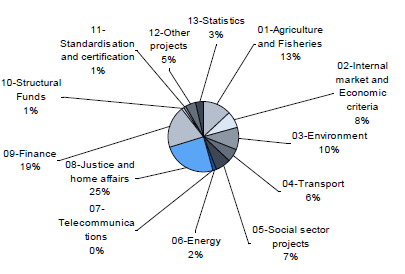
\includegraphics[width=4.5in]{Material/TwinningProjects}\\
Quelle: \cite{epec11}: 8.
\end{figure}
Aus dieser Grafik wird ersichtlich, dass der Anteil von Justice und Home Affairs 25\% an allen Twinning- und Twinning-Light-Projekten ausmachte. Überträgt man dies auf die in den Untersuchungsländern durchgeführten Projekte für die Jahre 2005-2008 (siehe Tabelle \ref{tab:AnteilTwinning}), kommt man auf maximal 3 Projekte pro Untersuchungsland, die dem Bereich Justice and Home Affairs zugeordnet sind. Es kann davon ausgegangen werden, dass es sich nicht in allen Fällen um Projekte zur Verwaltungsmodernisierung handelte, da auch die Modernisierung des Justizsystems unter diese Kategorie fällt. Für die Untersuchungsländer kann also festgehalten werden, dass Twinning, eines der Instrumente, das für Verwaltungsmodernisierung als besonders angemessen eingeschätzt wird, zumindest für die Zeit von 2005-2008 nur in geringem Umfang zum Einsatz kam.
\subsection{IPA – Instrument für Pre-Accession Assistance}
Das Programm IPA ersetzt die bis 2006 geltenden Instrumente PHARE, ISPA,\footnote{ISPA: Instrument for Structural Policies for Pre-Accession.} SAPARD,\footnote{SAPARD: Special Accession Programme for Agriculture \& Rural Development.} Heranführungshilfe für die Türkei und CARDS. Damit ist IPA seitdem das zentrale Instrument der Heranführungshilfe für die Beitrittsländer und die potenziellen Beitrittsländer in dem Prozess der Angleichung an die Standards der Europäischen Union zur Erlangung der Beitrittsreife.\par

Insbesondere soll das Instrument dazu beitragen:
\begin{itemize} \itemsep1pt \parskip0pt \parsep0pt
\item „die Demokratie und Rechtsstaatlichkeit zu stärken,
\item die öffentliche Verwaltung zu reformieren,
\item Wirtschaftsreformen durchzuführen,
\item die Menschen- und Minderheitenrechte zu achten,
\item die Gleichstellung der Geschlechter zu achten,
\item die Entwicklung der Zivilgesellschaft voranzubringen,
\item die regionale Zusammenarbeit sowie Versöhnung und Wiederaufbau zu fördern“ (\cite{senatskanzlei}). 
\end{itemize}
Grundlage für die Entwicklung von Projekten im Rahmen des IPA-Programmes sind folgende Dokumente:
\begin{itemize} \itemsep1pt \parskip0pt \parsep0pt
\item die Erweiterungsstrategie der Europäischen Kommission;
\item die jährlichen Fortschrittsberichte von der Europäischen Kommission. Für jedes (potenzielle) Beitrittsland von der Europäischen Kommission erstellt;
\item die Accession Partnerships (vgl. \cite{eurcom11a}).
\end{itemize}
Auf Basis dieser Dokumente werden mittelfristige Planungsdokumente, sog. Mehrjahresprogramme (über 3–4 Jahre), für jedes Land bzw. für mehrere Länder erstellt, die eine grobe Mittelaufteilung ausweisen, und je nach den Bedürfnissen jedes einzelnen Empfängerlandes für die fünf Komponenten des IPA-Instruments:
\begin{enumerate}[label=IPA {\Roman*}:,align=left,  leftmargin=*] \itemsep1pt \parskip0pt \parsep0pt
\item Übergangshilfe und Institutionenaufbau
\item  grenzübergreifende Zusammenarbeit
\item regionale Entwicklung (nur für Beitrittsländer)
\item Entwicklung der Humanressourcen (nur für Beitrittsländer)
\item ländliche Entwicklung.(nur für Beitrittsländer)
\end{enumerate}
Die Komponenten I und II werden durch die Kommission selbst oder durch die Delegationen der Kommission in den Empfängerländern verwaltet. Die Komponenten III bis V stehen nur den Beitrittsländern zur Verfügung und werden nach den Prinzipien der Strukturfondsförderung in den Empfängerländern mit den entsprechenden Verwaltungsstrukturen abgewickelt. Verwaltungsaufbau und Verwaltungsmodernisierung fallen unter Institutionenaufbau, also IPA I, und können durch das IPA-Programm in den drei Untersuchungsländern gefördert werden.\par
Neben der Förderung von Projekten in den einzelnen Ländern können auch länderübergreifende Programme im Rahmen von IPA umgesetzt werden. Aus der folgenden Tabelle wird die Finanzplanung pro Sektor für diese länderübergreifenden Programme deutlich:
\begin{table}[H]

\caption{Mehrjähriger indikativer Finanzrahmenplan 2011–2013, länderübergreifend.}
\small
\begin{tabular}{|L{56mm}|R{25mm}|R{25mm}|R{25mm}|}\hline
\multicolumn{4}{ |l| }{{\bf Indikative finanzielle Zuwendung pro Sektor (in Millionen EUR)}}\\\hline
&{\bf2007–2010}&\multicolumn{2}{c|}{\bf 2010–2013}\\\hline
Justiz und Innere Angelegenheiten, inkl. Grundrechte und vulnerable groups &285&24&4,61\%\\\hline
Öffentliche Verwaltung&60,92&38,5&7,39\%\\\hline
Zivilgesellschaft&40,5&30&5,76\%\\\hline
Entwicklung des privaten Sektors&123,9&70&13,44\%\\\hline
Transport und Energie Infrastruktur, inkl. Nukleare Sicherheit&124,45&108&20,73\%\\\hline
Umwelt und Klimawandel&16,3&17&3,26\%\\\hline
Soziale Entwicklung &71,98&96,5&18,52\%\\\hline
Andere Investitionen&173,86&96&18,43\%\\\hline
Reserve&0&40,97&7,86\%\\\hline
{\bf Gesamt}&{\bf 640,41}&{\bf 502,97}&{\bf 100\%}\\\hline
\multicolumn{4}{c}{}\\
\multicolumn{4}{c}{\normalsize Quelle: \cite{eurcom11b}: 15 (eigene Übersetzung aus dem Englischen).}
\end{tabular}
\\
\end{table}

Aus dieser Tabelle wird ersichtlich, dass für regionale, also länderübergreifende Programme im Bereich der öffentlichen Verwaltung für den Zeitraum 2011–13 Mittel in Höhe von 24 Millionen Euro zur Verfügung stehen. Diese werden im Balkan vor allem für die Unterstützung der regionalen Trainingseinrichtung für die öffentliche Verwaltung verwendet, die Regional School for Public Administration (RESPA), die 2010 in Montenegro eröffnet wurde.\par

„Gemäß den in den Mehrjahresprogrammen festgelegten Prioritäten werden für jedes Land in jährlichen Programmen konkret die Ziele, die Interventionsbereiche, die erwarteten Ergebnisse, die Verwaltungsverfahren und der für die Finanzierung vorgesehene Gesamtbetrag, eine Kurzbeschreibung der Art der zu finanzierenden Vorhaben, Angaben über die vorgesehenen Beträge je Vorhaben und ein vorläufiger Durchführungszeitplan festgelegt. Sobald die Programme im nicht-öffentlichen IPA-Programmausschuss durch die Vertreter der EU-Mitgliedstaaten genehmigt sind, erfolgen die Ausschreibungen.“\footnote{http://ec.europa.eu/enlargement/pdf/countries/ipa\_miff\_081106\_en.pdf (Aufgerufen 11.12.2012).}

Die Förderung durch IPA kann unterschiedliche Formen annehmen; dies sind vor allem:
\begin{itemize} \itemsep1pt \parskip0pt \parsep0pt
\item Zuschüsse zu öffentlichen Investitionen;
\item Unterstützung von Projekten der Zivilgesellschaft;
\item Twinning;
\item Direkte Budgethilfe (in Ausnahmefällen und unter Überwachung);
\item Technische Hilfe (\cite{epec11}: 2).
\end{itemize}
Für den Zeitraum 2007–2013 sind insgesamt Mittel in Höhe von 11,565 Milliarden. Euro vorgesehen (\cite{senatskanzlei}).\par


Für den Bereich Institutionenbildung, unter den die Verwaltungsmodernisierung fällt sind folgende Ausgaben in den Untersuchungsländern vorgesehen. 
\begin{table}[H]
\centering

\caption{ IPA 2007-13 Übergangshilfe und Institutionenaufbau (in Euro)}
\small
\begin{tabular}{|L{12mm}|R{16mm}|R{16mm}|R{16mm}|R{16mm}|R{16mm}|R{16mm}|R{16mm}|}\hline
&2007&
2008&
2009&
2010&
2011&
2012&
2013\\\hline
Maze\-donien&
41.641.613&
41.122.001&
39.328.499&
36.317.068&
28.803.410&
28.207.479&
27.941.228\\\hline
Monte\-negro&
27.490.504&
28.112.552&
28.632.179&
29.238.823&
29.843.599&
30.446.471&
30.996.035\\\hline
Alba\-nien&
54.318.790&
62.117.756&
71.377.079&
82.711.421&
84.301.650&
85.987.683&
87.446.037\\\hline
\multicolumn{8}{c}{}\\
\multicolumn{8}{c}{\normalsize Quelle: \cite{eurcom09b}.}
\end{tabular}
\end{table}
In einer Studie zur Implementierung von IPA Funds kommen die Autoren eines Think Tank in Mazedonien zu dem Ergebnis: „So far, it has been a general rule that the key roles in IPA program management for WB countries are fulfilled jointly by the central governments and the EU delegations to these countries. It has been observed that the participation of local authorities and Civil Society Organisations (CSOs) in the process of designing IPA priorities and drafting the national or local strategic documents has been limited. All WB candidate countries have encountered some common difficulties in dealing with IPA rules” (\cite{eurmov10}: 4).\par
Eine Studie zur Effektivität des IPA-Instrumentes, im Auftrag der EU durchgeführt, konstatiert die Erfolge des Instruments vor allem für Bereiche, die konkret im Acquis geregelt sind: „Effectiveness was judged to be strongest in those areas where actions are related to the alignment/adoption of the acquis, notably where the acquis is clearly defined in terms of a legal and administrative framework to be achieved”. Für Themen, die nicht konkret im Acquis definiert sind, so auch zum Thema Reform der öffentlichen Verwaltung, sehen die Evaluatoren das IPA-Programm kritischer: „Where the acquis is defined in a looser framework or there is not a formal acquis chapter (e.g. public administration), effectiveness is less evident. For this type of interventions the BENF needs to establish its own, appropriate strategic/implementation frameworks, often involving interagency cooperation” (\cite{htspe}: 37).\par
Eine andere Analyse des bisherigen IPA-Programmes gibt zu bedenken, dass schwache administrative Kapazitäten in den Kandidaten- und potenziellen Kandidatenländern dazu führen können Ressourcen zu binden, die anderswo nötiger und effektiver eingesetzt werden könnten: „Given the weak economic conditions, relatively fragile governance and underdeveloped administrative capacities in some beneficiaries, adopting EU standards at this stage may add significant costs to public activities and can inhibit the short-term competitiveness of productive activities” (\cite{epec11}: 3).\par
Eine weitere Problematik im Zusammenhang mit der IPA-Förderung generell, aber besonders für kleinere Länder wird in einer Entschließung des Europäischen Parlaments von 2011 zu Montenegro deutlich: „Das Europäische Parlament nimmt mit Zufriedenheit zur Kenntnis, dass die IPA-Hilfe in Montenegro gut funktioniert; fordert sowohl die Regierung Montenegros als auch die Kommission auf, das Verwaltungsverfahren für die Beantragung von IPA-Mitteln zu vereinfachen, damit diese für kleinere und dezentral organisierte Bürgerorganisationen, Gewerkschaften und andere Empfänger einfacher zugänglich sind“ (\cite{eurpar11}: o.S.). 

\subsection{Die SIGMA-Initiative der OECD }
\label{subsec:Die SIGMA-Initiative der OECD}

Von besonderer Bedeutung im Hinblick auf das Thema „Administrative Kapazitäten von Kandidatenländern“ ist die gemeinsame Initiative der Organisation für Ökonomische Zusammenarbeit und Entwicklung (OECD) und der Europäischen Kommission mit dem SIGMA-Programm (Support for Improvement in Governance and Management). SIGMA wurde 1992 gegründet, co-finanziert durch die EU. Ziel war es, die Länder Mittel- und Osteuropas bei der Modernisierung ihrer öffentlichen Verwaltungen zu unterstützen. In den späten 1990er Jahren entwickelte SIGMA Baseline-Kriterien, die Grundlage sind für die Betrachtung und Beurteilung der horizontalen administrativen Kapazitäten der Kandidatenländer. Diese OECD/SIGMA Baseline-Kriterien für die öffentliche Verwaltung sind: 
\begin{enumerate} \itemsep1pt \parskip0pt \parsep0pt
\item Policy-Entwicklung und Koordination 
\item Civil service und Verwaltungsrecht
\item Management der öffentlichen Ausgaben
\item Beschaffungswesen im öffentlichen Bereich
\item Interne Finanzkontrolle
\item Externe Rechnungsprüfung (vgl. \cite{cardona09}: 3).
\end{enumerate}
In der Arbeit legt SIGMA besonderen Wert darauf, den Austausch und die Zusammenarbeit von Regierungen zur Verwaltungsentwicklung zu fördern. Dazu gehört u.a. logistische Unterstützung für die Gründung von Netzwerken regionaler Verwaltungsspezialisten in Mittel- und Osteuropa und der Austausch dieser Experten mit solchen aus etablierten Demokratien. Weiterhin wird Informationsmaterial und Berichte über bestimmte Themen und Länder auf der OECD/SIGMA Website veröffentlicht. Es geht darum:
\begin{itemize} \itemsep1pt \parskip0pt \parsep0pt
\item den Reformfortschritt zu messen und Prioritäten zu identifizieren anhand Europäischer guter Praxis und bestehendem EU-Recht (Acquis communautaire). 
\item Unterstützung für Entscheidungsträger und Administratoren zur Verfügung zu stellen, für die Einrichtung der rechtlichen Rahmenbedingungen und Prozesse, um europäischen Standards und guter Praxis zu entsprechen.
\item EU-Finanzierung durch Hilfe beim Projektdesign und der Implementierung zu unterstützen (vgl. \cite{oecd99}: 2).
\end{itemize}
SIGMA veröffentlicht seit 1999 Länderberichte zu bestimmten Themen der Verwaltungsentwicklung. Diese werden von der Europäischen Kommission für ihre jährlichen Fortschrittsberichte zu den Kandidaten- und potenziellen Kandidatenländern verwendet.\par
Ohne konkretes EU-Modell zur Verwaltungsmodernisierung füllte die SIGMA-Initiative in gewisser Weise das Vakuum, das aufgrund fehlender klarer Bestimmungen auf EU-Ebene und der sich entwickelnden Konditionalität im administrativen Bereich entstanden war. Da die EU im Rahmen der Konditionalität kein allgemein gültiges Modell der öffentlichen Verwaltung zugrunde legt, bleibt es bei der allgemeinen Forderung der „ability to implement the acquis“. Dimitrova kritisiert, dass die EU nicht das Modell des New Public Management (NPM) zugrunde legt, das einflussreichste Paradigma der letzten Jahrzehnte in der Debatte um Verwaltungsmodernisierung. Stattdessen dient der EU ein weitgehend klassisches Weberianisches Modell der Bürokratie mit Etablierung eines professionellen (Berufs-) Beamtenapparates, der politisch unabhängig ist, als wesentlicher Orientierungspunkt (vgl. \cite{dimit05}: 81).

\subsection{Abgeschlossene Programme für den Westbalkan}
Herausragende bereits abgeschlossene Programme zur Heranführung beitrittswilliger Staaten an die EU-Standards sind die Tätigkeit der European Agency for Reconstruction (EAR) sowie die Programme PHARE und CARDS, die nachfolgend jeweils bezüglich der Verwaltungsmodernisierung kurz dargestellt werden.

\subsubsection{European Agency for Reconstruction}
Die European Agency for Reconstruction war für die Verwaltung der wesentlichen Unterstützungsprogramme der EU für Serbien, Kosovo (unter UN-Verwaltung), Montenegro und Mazedonien zuständig. Die EAR wurde gegründet, um die Wiederaufbauhilfe der EU für Kosovo zu koordinieren. Nach dem Fall des Milosevic-Regimes im Jahr 2000 wurde das Mandat auf Serbien und Montenegro und 2002 auf Mazedonien erweitert. Die EAR hatte ihre Zentrale in Thessaloniki (Griechenland) und Büros in Pristina (Kosovo), Belgrad (Serbien), Podgorica (Montenegro) und Skopje (Mazedonien). Bis zum Juli 2007 hat die EAR ca. 2,3 Milliarden Euro an Hilfe in den von ihr unterstützten Ländern ausgezahlt, wie aus folgender Tabelle ersichtlich:
\renewcommand{\arraystretch}{1}
\begin{table}[H]
\center
\setlength\belowcaptionskip{10pt}
\caption{Die Agency for Reconstruction (EAR). Zuwendungen bis Ende Juli 2007}
\small
\begin{tabular}{|L{25mm}|R{36mm}|R{36mm}|R{16mm}|}\hline
&
Bereitgestellt&
Ausgezahlt&
Quote\\\hline
Serbien&
1,3 Milliarden Euro&
921 Millionen Euro&
71\%\\\hline
Montenegro&
130 Millionen Euro&
104 Millionen Euro&
80\%\\\hline
Kosovo&
1,11 Milliarden Euro&
998 Millionen Euro&
90\%\\\hline
Mazedonien&
327 Millionen Euro&
259 Millionen Euro&
79\%\\\hline
Gesamt EAR&
2,86 Milliarden Euro&
2,3 Milliarden Euro&
80\%\\\hline
\multicolumn{4}{c}{}\\
\multicolumn{4}{c}{{\normalsize Quelle: \cite{zink}: 8 (eigene Übersetzung aus dem Englischen).}}
\end{tabular}
\end{table}
Aus dieser Tabelle ist ersichtlich, dass der überwiegende Teil der durch die EAR ausgezahlten Hilfe dem Kosovo zugute kam. Neben den Hauptempfängerländern Kosovo und Serbien erhielten Mazedonien und Montenegro 259 und 104 Millionen Euro respektive an Hilfsleistungen.\par
Außer zum Wiederaufbau hat die EAR im Laufe der Zeit auch für andere Bereiche Unterstützung zur Verfügung gestellt, z.B. für Projekte zur wirtschaftlichen Entwicklung, der Stabilisierung der administrativen Kapazitäten der geförderten Länder, im Justizsektor, der Zivilgesellschaft und im Bereich der Medien. Die EAR war dem Europäischen Parlament und dem Rat der Europäischen Union verantwortlich und arbeitete eng mit der Europäischen Kommission und ihren Vertretungen vor Ort zusammen. Im Dezember 2008 endete das Mandat der EAR und die Weiterführung der Förderprogramme ging an die EU-Delegationen in den unterstützen Ländern über (vgl. \cite{zink}: 10).

\subsubsection{PHARE}
Als Hauptinstrument der EU zur Heranführung der Kandidatenländer aus Zentral- und Osteuropa an die EU diente das PHARE-Programm.\footnote{Le phare (franz.) bedeutet Leuchtturm.} Dieses Programm war ursprünglich entwickelt worden, um Polen und Ungarn in Form von Wirtschaftshilfe bei der ökonomischen Umstrukturierung zu helfen, wurde aber später auf die anderen Beitrittskandidaten ausgedehnt (Bulgarien, Tschechische Republik, Estland, Lettland, Litauen, Slowakei, Slowenien und Rumänien). Einige Pilotprojekte in Polen und Ungarn zwischen 1995 und 1997 betrafen auch schon die administrative Kompetenz (\cite{tomtul}: 380). In einer schrittweise sich entwickelnden Heranführungsstrategie standen in der Zeit ab 1996 PHARE, Beitrittspartnerschaften, und Nationale Programme für die Anpassung an den Acquis zur Verfügung. Von dieser Phase an waren neben der Infrastruktur, rechtlicher und ökonomischer Angleichung auch die administrativen Kapazitäten der Beitrittsländer im Blick der EU. 1997 beschloss die EU-Kommission die „Agenda 2000“ und schlug vor, die Hilfen zu 30\% für Institutionenbildung und 70\% für Investitionen zur Verfügung zu stellen. Die Abordnung nationaler Experten der Kandidatenländer zu Schulungszwecken (TAIEX) und von Beamten der EU-Mitgliedsländer in die Kandidatenstaaten (Twinning) wurde als Instrument der Verwaltungsentwicklung und -unterstützung entwickelt (\cite{lipumb04}: 60).\par

Als Ziele des PHARE-Programmes nennt die EU auf ihrer Website:
\begin{itemize}
\item „helping the administrations of the candidate countries to acquire the capacity to implement the Community acquis. PHARE also helps the national and regional administrations, as well as regulatory and supervisory bodies, in the candidate countries to familiarise themselves with Community objectives and procedures;
\item helping the candidate countries to bring their industries and basic infrastructure up to Community standards by mobilising the investment required, particularly in areas where Community rules are increasingly demanding: environment, transport, industry, product quality, working conditions etc.”\footnote{http://europa.eu/legislation\_summaries/enlargement/2004\_and\_2007\_enlargement/e50004\_en.htm (Aufgerufen: 19.8.2012).}
\end{itemize}
In einer Evaluierung von PHARE-Projekten zur Verwaltungsmodernisierung in fünf Beitrittsländern\footnote{Estland, Lettland, Litauen, Polen und Slowakei.} wurden Projekte aus den Bereichen gesetzgeberische und organisatorische Reformen des civil service, Training für öffentlich Bedienstete und Verbesserung der IT-Infrastruktur untersucht. Die Ergebnisse sind schematisch in folgender Tabelle dargestellt:
\renewcommand{\arraystretch}{1}
 \begin{table}[H]
\center

\caption{Evaluierung von PHARE-Projekten zur Verwaltungsmodernisierung in CEE}
\small
\begin{tabular}{|L{40mm}|C{14mm}|C{14mm}|C{14mm}|C{14mm}|C{14mm}|C{14mm}|}\hline
&Anzahl Projekte&Efficiency&Effectiveness&Impact&Nachhaltigkeit&Durchschnitt\\\hline\hline
{\bf Land}&\multicolumn{6}{|r|}{}\\\hline
Estland&3&2,3&2,3&2&1,7&2,1\\\hline
Lettland&9&3,6&3,2&2,9&2,3&3\\\hline
Litauen&10&2,7&2,1&1,8&1,5&2\\\hline
Polen&15&3,8&3,5&2,3&2,1&3\\\hline
Slowakei&3&3&2,7&2,7&2,3&2,7\\\hline\hline
{\bf Projektarten}&\multicolumn{6}{|r|}{}\\\hline
Rechtliche und orga- nisatorische Reformen&30&3,3&2,9&2,3&1,9&2,6\\\hline
Weiterbildung/Training&5&3,6&3,4&3,2&3&3,3\\\hline
Informationstechnologie&5&3,2&2,8&1,8&1,6&2,4\\\hline\hline
{\bf Zuwendungs-\newline empfänger}&\multicolumn{6}{|r|}{}\\\hline
Zentrale Exekutive&18&2,9&2,1&1,8&1,7&2,1\\\hline
Lokale Exekutive&13&3,7&3,7&2,8&2,2&3,1\\\hline
Lokale und Zentrale Exekutive&6&3,5&3,5&2,5&2,2&2,9\\\hline
Parlament&3&3,7&3,7&2,7&2,7&3,2\\\hline\hline
{\bf Durchschnitt (alle Projekte)}&40&3,3&3&2,3&2&2,6\\\hline\hline
\multicolumn{7}{|r|}{1 (sehr schlecht), 2 (eher schlecht), 3 (angemessen), 4 (gut), 5 (sehr gut)}\\\hline
\multicolumn{7}{c}{}\\
\multicolumn{7}{c}{\normalsize Quelle: \cite{ips}: 96}\\
\multicolumn{7}{c}{ (\normalsize eigene Übersetzung aus dem Englischen).}
\end{tabular}
\end{table}
\renewcommand{\arraystretch}{1.2}

Aus dieser Tabelle ist ersichtlich, dass im Bereich der größten Anzahl der Projekte, bei rechtlichen und organisatorischen Reformen des civil service (30 Projekte), die Nachhaltigkeit nicht ausreichend gegeben war.

Zur Analyse der Gründe für das generell schlechte Abschneiden der untersuchten Projekte werden mehrere Faktoren benannt. Ein wesentlicher Faktor wird von den Evaluatoren darin gesehen, dass es entweder keine strategische Ausrichtung der PAR-Projekte gab, oder diese häufigen Veränderungen unterlag. Weiterhin war die Projektentwicklung oft extern vergeben und hat die konkreten Bedingungen vor Ort nicht ausreichend berücksichtigt. Die Auswahl der Projekte war ad-hoc und „demand driven“, PAR war dagegen „project driven” mit starkem Gewicht auf inputs (Unterstützung durch Experten und Bereitstellung von Equipment) und wenig Augenmerk auf outputs und impact. Während die Autoren der Evaluierung viele der identifizierten Probleme den Turbulenzen der frühen Jahre der Transition zurechnen, mahnen sie Verbesserungen im Management der Unterstützungsprogramme an (vgl. \cite{ips}: 98).

Die Autoren der Evaluation schließen mit einer Empfehlung an die EU-Kommission: 

„The Commission is urgently in need of some criteria:
\begin{itemize}
\item against which a rational discussion of PAR issues can be held, even if these discussions cannot form a formal part of the accession negotiations;
\item that would offer some guidance and policy focus for PHARE PAR programmes” (\cite{ips}: 103).
\end{itemize}
Für die Länder des Westbalkans wurde das PHARE-Programm im Jahr 2000 durch ein neues Instrument, CARDS, abgelöst.


\subsubsection{CARDS} 

Die wirtschaftliche, politische und soziale Zusammenarbeit der EU mit den Ländern des Westlichen Balkans wurde mit dem Hilfsprogramm „Community Assistance for Reconstruction, Democratization and Stabilization“ (CARDS) als neuem Instrument umgesetzt. CARDS war Teil der Stabilisierungs- und Assoziierungsstrategie der Europäischen Union gegenüber dem Westlichen Balkan, und im Rahmen des SAP wurden Mittel unter CARDS abrufbar. Ab dem Jahr 2000 wurden Mittel der EU bereitgestellt, um Reformprozesse in den Zielländern zu unterstützen (vgl. \cite{calic01}: 12).\par

Die drei Untersuchungsländer der vorliegenden Arbeit (Albanien, Mazedonien und Montenegro) profitierten ab 2000 von CARDS, das bis 2006 zur Verfügung stand. Die Zuständigkeit für das CARDS-Programm wechselte im Jahr 2005 von einer gemeinsamen Zuständigkeit der Generaldirektion Außenbeziehungen und des Europäischen Amtes für Entwicklungszusammenarbeit „EuropeAid“ hin zur Generaldirektion Erweiterung (vgl. \cite{eurrh}: C285/5).\par
Die Gelder aus dem CARDS-Programm standen für verschiedenste Zwecke zur Verfügung, z.B. für Infrastrukturprojekte, Hilfe für Flüchtlinge, Institutionenbildung und Polizeikooperation. Fast die Hälfte des Geldes war für Serbien/Montenegro bestimmt, vor allem aufgrund der Situation im Kosovo. In Mazedonien und Montenegro war ab 2003 die European Agency for Reconstruction (EAR) für die Verwaltung des Programmes zuständig. In Albanien wurde CARDS von der Delegation der Europäischen Kommission in Tirana verwaltet. Regionale Projekte wurden direkt von Brüssel unterstützt. Der Anteil des tatsächlich verausgabten Geldes unterscheidet sich für die Untersuchungsländer. Montenegro hatte eine Absorptionsrate von 86\%, Mazedonien 52\% und Albanien rangiert am unteren Ende mit 29\%. (vgl. \cite{inotai}: 42). Insgesamt wurden von der EU in den Jahren 2000–2006 unter CARDS 4,6 Milliarden Euro zur Verfügung gestellt (vgl. \cite{mus}: 13). Der Europäische Rechnungshof kommt in einer Evaluierung des CARDS-Programmes zu dem Ergebnis, dass vor allem Infrastrukturmaßnahmen erfolgreich umgesetzt wurden, während CARDS bei der Verbesserung der staatlichen Verwaltungskapazitäten weniger effektiv war. Gründe werden vor allem darin gesehen, dass der Schwerpunkt ursprünglich nicht auf dem Institutionenaufbau lag und die Empfängerländer keine ausreichenden Kapazitäten zur Absorption der Hilfe hatten (vgl. \cite{eurrh}: C285/15).
\begin{table}[H]

\center
\caption{CARDS Mittelzuweisungen Albanien, Mazedonien (2002-2006) und Montenegro (2005-2006), nach Sektoren in Millionen Euro}
\small
\begin{tabular}{|L{60mm}|R{13mm}|R{13mm}|R{13mm}|R{13mm}|}\hline
{\bf Albanien} &{\bf 2002} &{\bf 2003} &{\bf 2004} &{\bf 2005-6}\\\hline
Justice \& Home Affairs&21&20&35&27\\
Administrative Capacity Building&6&8&4&23\\
Economic \& Social Development&12,9&17,5&12&31\\
Environment, Natural Resources&4&-&10&-\\
Democratic Stabilisation&1&1&2,5&4\\\hline
\end{tabular}
\begin{tabular}{|L{60mm}|R{13mm}|R{13mm}|R{13mm}|R{13mm}|}\hline
{\bf Mazedonien} &{\bf 2002} &{\bf 2003} &{\bf 2004} &{\bf 2005-6}\\\hline
Justice \& Home Affairs&7&12,5&24&17\\
Administrative Capacity Building&14&9&8,5&24\\
Economic \& Social Development&11,5&11&15&20\\
Environment, Natural Resources&-&1&2&3\\
Democratic Stabilisation&3&3&3&2\\\hline
\end{tabular}
\begin{tabular}{|L{60mm}|R{13mm}|R{13mm}R{13mm}R{13mm}}\cline{1-2}
{\bf Montenegro} &{\bf 2005-6}\\\cline{1-2}
Justice \& Home Affairs&3&&&\\
Administrative Capacity Building&11&&&\\
Economic \& Social Development&16,3&&&\\
Environment, Natural Resources&6&&&\\
Democratic Stabilisation&3,7&&&\\\cline{1-2}
\multicolumn{5}{c}{}\\
\multicolumn{5}{C{114mm}}{Quelle: http://ec.europa.eu/enlargement/how-does-it-work/}\\
\multicolumn{5}{C{114mm}}{financial-assistance/cards/statistics2000-2006\_en.htm}\\
\multicolumn{5}{C{114mm}}{ (Aufgerufen: 5.5.2010).}
\end{tabular}
\end{table}

Aus den Tabellen wird ersichtlich, dass für die beiden Jahre 2005 und 2006 in Albanien und Mazedonien ein starker Anstieg der Ausgaben im Bereich Administrative Capacity Building stattgefunden hat. In einer Evaluation des CARDS-Programmes für Albanien wird dennoch konstatiert, dass die die Erfolge des Programmes im Bereich Verwaltungsunterstützung moderat waren: „Support to public administration has been limited in terms of both the number of projects and project size, and a proprer public administration reform and civil service reform have not been implemented“ (\cite{cowi}: ii). Für Montenegro ist die Darstellungsweise erst ab 2005/6 gegeben, wohl aufgrund der Darstellung zusammen mit Serbien bis zur staatlichen Unabhängigkeit 2006. 

\subsection{Zwischenergebnis für die Verwaltungsmodernisierung}
Betrachtet man die theoretischen Ansätze, die praktische Entwicklung und die gezielten Förderprogramme im Zusammenhang, so wird erkennbar, dass trotz der Erfahrungen der EU mit der Osterweiterung, die Verwaltungsmodernisierung und der Status der Verwaltung in den Beitrittsländern nicht angemessen berücksichtig wird. In den Förderprogrammen für den Westlichen Balkan werden regelmäßig Mittel auch für die Modernisierung der öffentlichen Verwaltung bereitgestellt. In Abwesenheit einer glaubhaften Konditionalität und einer Verankerung des Themas im Acquis communautaire sind kritische Evaluationen der bisherigen Förderprogramme in Bezug auf Verwaltungsentwicklung im Balkan allerdings nicht verwunderlich. Es entsteht der Eindruck, dass die EU das Thema Verwaltungsmodernisierung zwar immer wieder als wichtig darstellt, z.B. in den jährlichen Fortschrittsberichten, aber keine operationalisierbaren Instrumente entwickelt hat zu einer nachhaltigen Förderung einer modernen Verwaltung. \par
Dies ist umso erstaunlicher, als die fehlende Modernisierung der öffentlichen Verwaltung in den Ländern der letzten Erweiterungswelle wie gezeigt wurde von der Forschung deutlich herausgearbeitet wurde.\par
Um ein möglichst genaues Bild des Status quo des aktuellen Standes der Verwaltungsentwicklung in den drei Untersuchungsländern zu erhalten, wird im Folgenden der Blick erweitert um die historische Entwicklung der öffentlichen Verwaltung.




%\chapter{Expertenbefragung zur Verwaltungsentwicklung}
Nach der Auswertung der Literatur zur Problematik der Verwaltungsmodernisierung im Westbalkan und der Herausarbeitung des Einflusses, den die EU-Erweiterung auf die Verwaltungsentwicklung hat, sowie der detaillierten Betrachtung von historischen Legacies, die möglicherweise bis in die heutige Zeit nachwirken, werden nun anhand von Experteninterviews die offenen Fragen zur weiteren Entwicklung betrachtet. Dieser Einblick in die Praxis der Verwaltungsmodernisierung im Erweiterungsprozess liefert zusätzliche Erkenntnisse zur Beantwortung der Untersuchungsfragen der vorliegenden Arbeit.\par
Die vorrangig klärungsbedürftig erscheinenden Fragen wurden zu einem Interviewleitfaden gebündelt, der auf der Grundlage der vorherigen Literaturauswertung erstellt wurde. Der Leitfaden enthält die Fragen, die beantwortet werden sollen, und stellt eine Art Richtschnur für den Interviewer dar. Der Interviewleitfaden soll ein allzu weites thematisches „Abdriften“ während des Interviews vermeiden und dennoch Flexibilität in der Gesprächsführung ermöglichen. Aufgrund dieser Spielräume bei der konkreten Gestaltung des Interviews, bei dem gleichzeitigen Versuch alle zu behandelnden Themen unterzubringen, werden solche Interviews gelegentlich auch als „teilstandardisierte Interviews“ bezeichnet (vgl. Flick 2010: 223).\par
Die Klassifizierung von Interviews ist dem folgenden Schema zu entnehmen, wobei das halbstandardisierte Interview im Wesentlichen dem teilstandardisierten Interview entspricht:

\begin{table}[H]
\caption[Interviewtypen in der qualitativen Sozialforschung]{Interviewtypen in der qualitativen Sozialforschung}
\center
\scriptsize{
\begin{tabular}{|L{40mm}|L{40mm}|L{40mm}|}\hline
&Fragewortlaut und -reihenfolge&Antwortmöglichkeiten\\\hline
Standardisiertes Interview&
Vorgegeben&
Vorgegeben\\\hline
Halbstandardisiertes Interview&
Vorgegeben&
Nicht vorgegeben\\\hline
Nichtstandardisiertes Interview&
Nicht vorgegeben (nur Thema)&
Nicht vorgegeben\\\hline
\end{tabular}\\
\vspace{0,5cm}
Quelle: Gläser/Laudel 2010: 41. 
}
\end{table}
 
Diese Tabelle stellt die unterschiedlichen Herangehensweisen zur Interview-Durchführung im Überblick dar. Das für die vorliegende Untersuchung gewählte Verfahren der halbstandardisierten Durchführung arbeitet mit vorgegebenen Fragen in einer von der Interviewerin vorher festgelegten Reihenfolge. Die Antwortmöglichkeiten sind allerdings nicht vorgegeben und der Interviewte hat viel Raum, die persönliche Sichtweise und Einschätzung einfließen zu lassen. Es kann daher auch zu Überlappungen in der Beantwortung der Fragen durch den Interviewten kommen, die in der Auswertung und thematischen Zuordnung der Antworten zu berücksichtigen sind.
\section{Themen der Expertenbefragung} 
Thematisch wird an die zentralen Untersuchungsfragen sowie an die bisherigen Auswertungsergebnisse angeknüpft. Mit den Experteninterviews wird eine weitere Sichtweise in die Untersuchungen einbezogen, mit der die bisherigen Ergebnisse im Sinne des methodischen Konzepts der Triangulation ergänzt, unterstützt, aber auch relativiert werden können.\par
Für die Interviews ist zunächst ein Überblick sinnvoll über die Einschätzungen der Interviewpartner zur Bedeutung von Verwaltungsmodernisierung im Zusammenhang mit der Erweiterungsdebatte. Wie schon erörtert wurde, ist die Verwaltungsmodernisierung kein eigenständiges Kapitel des Acquis. Dennoch ist eine leistungsfähige öffentliche Verwaltung notwendig, um die einzelnen Aufgaben bei der Übernahme des Acquis vor dem Beitritt zur EU zu organisieren und durchzuführen. Auch die Verwaltung der EU-Förderprogramme vor dem Beitritt erfordert einen öffentlichen Sektor, der bestimmten Mindeststandards entspricht.\par
Hierzu wurde folgende Frage gestellt:\par
\begin{itemize}[label={}]
\item \ul{Public Administration Reform is not a separate chapter in the Acquis. Should it be a separate chapter?}
\end{itemize}
Neben der Bedeutung der öffentlichen Verwaltung im Beitrittsprozess sind die hemmenden und die fördernden Faktoren für die Verwaltungsentwicklung auf dem Westbalkan von Interesse. Hierzu wurde folgende Frage gestellt:
\begin{itemize}[label={}]
\item \ul{In your opinion, are there obstacles to PAR in Albania, Macedonia and Montenegro? And what would be necessary for successful PAR in Albania, Macedonia and Montenegro?}
\end{itemize}

Speziell sind in diesem Zusammenhang auch die Einschätzungen der Experten von Interesse zur Bedeutung der nachwirkenden historischen Verfahrensweisen sowie zur Übertragbarkeit von Erfahrungen aus früheren Beitrittswellen. Hierzu wurden folgende Fragen gestellt:
\begin{itemize}[label={}]
\item \ul{The literature on enlargement sometimes argues with the legacy theory, in particular regarding the last wave of enlargement. Meaning that structures of previous regime set-ups have an influence on the present development of Public Administration Reform. What is your view on this issue regarding Albania, Macedonia and Montenegro?}
\item \ul{Do you perceive differences in the EU approach compared with the experience with PAR during the last wave of enlargement?}
\end{itemize}
Weitere Fragen zur Verwaltungsmodernisierung betreffen die aktuellen (Finanz-)Programme der EU. Die Förderinstrumente, die im Rahmen der Erweiterungsstrategie zur Verfügung stehen, sind entwickelt und weiterentwickelt worden, um die (potenziellen) Kandidatenländer bei der Übernahme des Acquis communautaire zu unterstützen. Fraglich ist, ob diese aus Sicht der Experten dem Bedarf gerecht werden. Hierzu wurden folgende Fragen gestellt:
\begin{itemize}[label={}]
\item \ul{Which topics/areas are presently dealt with as a priority by the EU regarding Public Administration Reform in Albania, Macedonia and Montenegro? What are the developments you see there?}
\item \ul{Do you think the EU approach regarding Public Administration Reform in Albania, Macedonia and Montenegro is adequate? Or should other aspects be included from your point of view?}
\item \ul{How do you assess the EU-Instruments to promote Public Administration Reform in Albania/Macedonia and Montenegro as regards quantity and effectiveness:
Differentiate per country, if possible}
\begin{itemize}
\item CARDS (phased out)
\item Twinning
\item Twinning light
\item TAIEX
\item IPA
\end{itemize}
\item \ul{Are these programmes well designed for the needs of PAR in Albania/Macedonia and Montenegro or do you perceive a need for adjustment in any of them? (Content or technical)}
\end{itemize}

Das Thema Verwaltungsmodernisierung wird von verschiedenen Abteilungen der EU-Kommission bearbeitet. Ihre wesentlichen Aufgaben sind die jährliche Berichterstattung und die Umsetzung von Projekten zur Verwaltungsmodernisierung in den Zielländern. In den Untersuchungsländern selbst sind die Zuständigkeiten für das Thema Verwaltungsmodernisierung ebenfalls unterschiedlich ausgestaltet. Hierzu wurden folgende Fragen an die Experten gestellt:
\begin{itemize}[label={}]
\item \ul{How do you assess the cooperation within the EU Commission regarding Public Administration reform in Albania, Macedonia and Montenegro with the different Units, DG Enlargement, country desks, special PAR Unit and DG Admin?}
\item \ul{Who is responsible for co-ordinating the PAR activities of all the different donors in Albania, Macedonia and Montenegro and what is happening in this respect at the moment? }
\end{itemize}

\subsection{Auswahl der befragten Experten}
Den ausgewählten Themen entsprechend wurden die zu befragenden Experten ausgewählt. „Als Experten könnte man diejenigen Personen bezeichnen, die in Hinblick auf einen interessierenden Sachverhalt als ‚Sachverständige’ in besonderer Weise kompetent sind“ (Deeke 1995: 7). Bei Experteninterviews interessiert der Befragte weniger in seinem biographischen Zusammenhang, sondern mehr in seiner Eigenschaft als Experte in einem bestimmten Handlungsfeld. Er wird auch nicht als Einzelfall, sondern als Repräsentant einer Gruppe betrachtet (vgl. Flick, 2010: 214). Es soll im Rahmen der empirischen Generalisierung Repräsentatives, aber auch Unerwartetes herausgearbeitet werden. Ziel ist es, das „überindividuell Gemeinsame herauszuarbeiten, Aussagen über Relevanzstrukturen, Wirklichkeitskonstruktionen, Interpretationen und Deutungsmuster zu treffen“ (Meuser/Nagel 2002: 80).\par
Da es sich um drei verschiedene Untersuchungsländer handelt, ist es erforderlich, aus jedem Staat Experten einzubeziehen. Es wurden pro Untersuchungsland jeweils ein Vertreter der Regierung bzw. der Verwaltung und ein Vertreter einer NGO befragt. Alle Interviewten hatten im sich im Rahmen ihrer beruflichen Tätigkeit intensiv mit dem Thema öffentliche Verwaltung und EU-Erweiterung in dem jeweiligen Land beschäftigt. Die NGO-Vertreter wurden einbezogen in der Annahme, dass sich aus der Sicht von Vertretern der Zivilgesellschaft andere Sichtweisen und andere Einschätzungen ergeben als bei den befragten Regierungs- und Verwaltungsvertretern. Somit wurde versucht eine größere Bandbreite an nationalen Einschätzungen zu erreichen. Die Auswahl auf NGOs als Experten fiel auch aufgrund der Vorannahme, dass Kritik im Rahmen eines Interviews eher von NGOs als von den Verantwortlichen der nationalen Regierung oder Verwaltung verbalisiert werden würde. In den drei Untersuchungsländern wurden NGOs ausgewählt, die sich in ihrer Arbeit theoretisch und praktisch mit der EU-Förderung der Verwaltungsentwicklung in dem jeweiligen Land beschäftigt haben.\par
Daneben wurden weitere sechs Experten aus dem Kontext der EU – EU-Kommission DG Enlargement (5) und OECD/SIGMA (1) – berücksichtigt. Diese Interviewpartner sind in verschiedenen Bereichen mit dem Thema öffentliche Verwaltung und EU-Erweiterung befasst, sie werden im Rahmen der vorliegenden Untersuchung als „EU officials“ bezeichnet.\par
Als Experten der EU-Kommission wurden Vertreter des DG Enlargement aus den drei Country-Desks für Albanien, Mazedonien und Montenegro ausgewählt. Diese beschäftigen sich auch unter politischen Gesichtspunkten mit der Verwaltungsenwicklung und verfassen u.a. die jeweiligen Kapitel in den jährlichen EU-Fortschrittsberichten. Weiterhin wurde ein Vertreter der Stabsstelle Verwaltungsmodernisierung und ein Mitglied der Evaluierungsstelle des DG Enlargement als Interviewpartner ausgewählt. Diese beiden Interviewpartner beschäftigen sich mit der Auswertung von Programmen der EU zum Thema Verwaltungsentwicklung in den Kandidatenländern. Bei der OECD konnte ein hochrangiger Vertreter des SIGMA-Programmes als Interviewpartner gewonnen werden. SIGMA erstellt im Auftrag der EU-Kommission Berichte zu verschiedenen Themen der Verwaltungsmodernisierung in den Beitrittsländern\footnote{Näheres zum SIGMA-Prgramm der OECD siehe Abschnitt 2.4.3 dieser Arbeit.}. Eine Liste der Interviews mit Angabe von Ort und Zeit der Durchführung ist als Anhang yy beigefügt. Eine Liste mit den Namen der befragten Experten liegen der Erstgutachterin und dem Zweitgutachter der Arbeit vor, sind aber aus Datenschutzgründen nicht in der veröffentlichten Version der Arbeit enthalten.\par
Es wurde ein Leitfaden erstellt für die Interviews mit den EU officials und ein leicht abgewandelter Leitfaden für die Gesprächspartner in den Untersuchungsländern. Der Leitfaden für die Durchführung der Interviews mit EU officials wurde von Herrn Professor Dr. Karl-Heinz Mintken (MPA-Studienbetreuung an der Universität Kassel) und Dr. Jan Kruse (Institut für Soziologie, Universität Freiburg) dankenswerterweise gelesen und mit Kommentaren versehen. Dies führte zu einer überarbeiteten Form der beiden Interviewleitfäden (siehe Anhang xx, xx)\footnote{Die Zweckmäßigkeit des Leitfadens für die Durchführung der Interviews wurde von der Verfasserin mit einem ihr bekannten deutschen Experten in einem Probeinterview geprüft. Das Testinterview diente als „Generalprobe“ sowohl für die inhaltliche als auch für die zeitliche und die technische Komponente der Interviewdurchführung. Der Experte, der dankenswerterweise für dieses Testinterview zur Verfügung stand, ist Jurist und Verwaltungsfachmann; er war vor einigen Jahren in Montenegro am Aufbau einer unabhängigen State Audit Institution (SAI) – einer Art Rechnungshof – im Rahmen eines GTZ-Projektes beteiligt. }.

\subsection{Durchführung der Interviews} 
Wichtig für das Ergebnis einer Befragung könnte auch die Wahrnehmung des Interviewers durch den Experten sein. Idealerweise wird von der Offenheit der Gesprächsführung und der Neutralität des Interviewers ausgegangen. Dem steht die reale Situation des Gespräches gegenüber mit mannigfachen potenziellen Erwartungen, Störungen und Übertragungen auf beiden Seiten. Ein Autor beschreibt die Interviewsituation anschaulich als ein „Drama“, in dem Sicht- und Erfahrungsweisen des Interviewpartners eine Bühne geschaffen wird, mit dem Befragten in seiner thematischen und persönlichen Selbstdarstellung und dem Interviewer in seiner Rolle als aktiver und permissiver Zuhörer, der den anderen angemessen und ausreichend zu Wort kommen lässt und ihn dabei unterstützt und fördert (vgl. Hermanns 2000: 376). Gewissermaßen handelt es sich bei der Interviewsituation um einen reflexiven Prozess: „Qualitative Interviews (und darüber hinaus alle empirische Forschungsmethoden) bilden nicht ‚Wahrheit’ ab, sondern komplexe Kommunikationsprozesse, in denen ‚Daten’ überhaupt erst produziert werden. Es geht um die Aushandlung von kommunikativem Sinn, der gemeinsam hergestellt wird; es geht um Fremdverstehensprozesse, in denen soziale Wirklichkeit interaktiv und koproduktiv hergestellt wird“ (vgl. Kardoff 1995, zit. in Kruse 2011: 109). Bogner und Menz entwickelten zu der Beziehung zwischen Interviewer und Befragtem und den Implikationen für die Interviewsituation folgende Typologie:
\begin{figure}
\caption{Kommunikative Merkmale von Interviewsituationen}
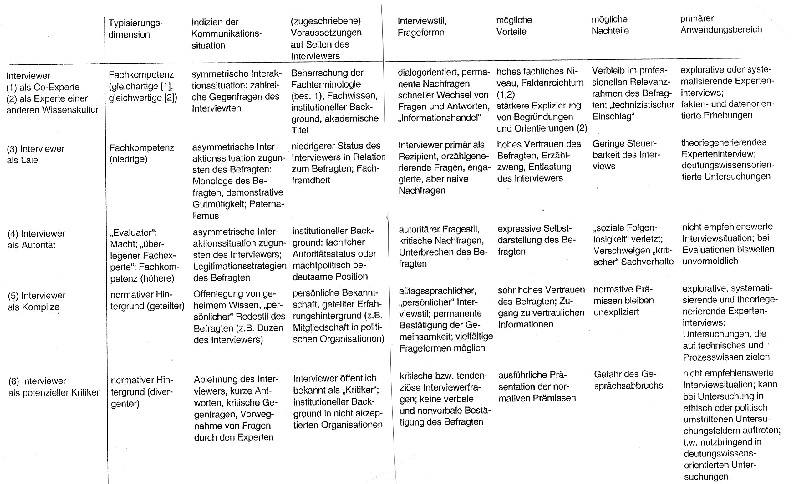
\includegraphics[width=5in]{Material/BognerMenz}\\
\scriptsize{Quelle: Bogner/Menz 2002: 63.}
\end{figure}
Aus dieser tabellarischen Übersicht wird deutlich, dass der Interviewer in der Interviewsituation eine oder mehrere Rollen einnimmt, bzw. vom Interviewten in unterschiedlichen Rollen wahrgenommen wird. Dies geschieht meist unbewusst und hängt von verschiedenen Faktoren ab. Da sich diese Wahrnehmung aber ggf. auf die Ergebnisse auswirkt, ist es hilfreich sich als Interviewer über die jeweils eingenommenen Rollen oder Rollenzuschreibungen klar zu werden. \par
In der von der Verfasserin durchgeführten Befragung entstand bei der Interviewerin der Einduck, dass sie von den Experten vornehmlich in einer Position wahrgenommen wurde, die zwischen den beiden Polen Co-Experte und Laie der obigen Einteilung oszillierte. Um Beeinträchtigungen des Ergebnisses der Expertenbefragung durch unterschiedliche Interviewer und deren unterschiedliches Verhalten zu vermeiden, hat die Verfasserin alle Interviews anhand eines strukturierten Gesprächsleitfadens selbst durchgeführt und selbst transkribiert.\par
Die für die vorliegende Arbeit verwendeten Interviews wurden in einem Fremdsprachenkontext durchgeführt. Die Interviewerin und der Interviewte hatten in 10 der 12 Fälle nicht die gleiche Muttersprache und auch hinsichtlich des unterschiedlichen kulturellen Kontextes ergibt sich eine besondere Situation. Die besondere Problematik hinsichtlich des kommunikationstheoretischen und analytischen Umgangs in der Durchführung und Auswertung von Interviews im fremdsprachlichen Kontext wurde in der Literatur methodisch noch kaum bearbeitet (vgl. Kruse 2011: 121). Um eine gemeinsame Kommunikationsbasis herzustellen, wurden die Interviews auf Englisch durchgeführt, anhand eines ebenfalls auf Englisch ausgearbeiteten Leitfadens\footnote{Das Interview mit dem Official in Montenegro wurde mit einem Übersetzer für Englisch durchgeführt, da die Interviewerin kein Serbo-Kroatisch und der Interviewte kein Englisch sprach. Die Durchführung des Interviews unterschied sich von den anderen durchgeführten Interviews nur durch die Anwesenheit eines Übersetzers, der die Fragen und Antworten konsekutiv übersetzte.}. Während dieses Zurückgreifen auf eine gemeinsame Drittsprache einerseits problematisch ist, sieht Kruse auch einen möglichen Vorteil in dieser Sprachwahl-Konstellation. Während der Befragte auf der einen Seite eine Einschränkung seines gewohnten Sprachausdrucks erlebt, eröffnet sich ihm auf der anderen Seite gleichzeitig auch die Freiheit, sich außerhalb der gewohnten idiomatischen Systeme der Muttersprache auszudrücken (vgl. Kruse 2011: 123). \par
Als Zeitschätzung, die auch in einem Probeinterview getestet wurde, war eine Stunde zur Durchführung eines Interviews vorgesehen. Während diese Zielvorgabe für die Mehrzahl der Interviews eingehalten wurde, dauerte ein Interview nur knapp 30 Minuten, zwei Interviews dauerten dagegen länger als eineinhalb Stunden. Die Fragen wurden den Interviewten nicht vor dem Interview zur Verfügung gestellt und auch nicht schriftlich vorgelegt. Alle Interviewten beantworteten die Fragen am Tag des Interviews, ohne diese vorher zu kennen. Die Interviews wurden mit einem digitalen Aufnahmegerät aufgezeichnet. Ein Interview wurde nicht aufgenommen, weil der Interviewte Vorbehalte gegen die Aufzeichnung hatte. In diesem Fall wurde eine handschriftliche Mitschrift durch die Interviewerin angefertigt. Alle transkribierten Interviews in ganzer Länge sowie die von der Autorin vorgeschlagene Auswahl an Textstellen zur Weiterverarbeitung im Forschungszusammenhang wurden der/dem jeweils Interviewten zugesandt und von ihm/ihr autorisiert. Jedem Interviewten wurde nur ihr/sein eigenes Interview vorgelegt.\par
Die durchgeführten Interviews wurden von der Autorin, unter Beibehaltung der englischen Sprache transkribiert. Dieses Vorgehen wurde gewählt, um Interpretations- und Deutungsverluste durch eine Übersetzung zu vermeiden. Aus dem gleichen Grund wurden die Interviews nicht in die deutsche Sprache übersetzt. Eine Zusammenstellung der für die Auswertung ausgewählten Interviewabschnitte ist als Kompilation pro Frage in \ref{}Anhang xx beigefügt.

\subsection{Auswertung der Interviews}
Für die Auswertung des gewonnenen Materials hat sich in der qualitativen Sozialforschung eine Reihe von Methoden und Verfahren herausgebildet, die meist ohne Systematisierung nebeneinander gestellt und unabhängig voneinander beschrieben werden. Von Gläser / Laudel werden unterschieden:
\begin{itemize}
\item Freie Interpretation
\item Sequenzanalytische Verfahrensweise
\item Grounded theory (Kodieren)
\item Qualitative Inhaltsanalyse
\end{itemize}

\begin{figure}
\caption{Überblick zu Verfahren der Interviewauswertung in den Sozialwissenschaften}
\includegraphics[width=5in]{Material/KlassifizierungAuswertungsmethoden}\\
\scriptsize{Quelle: Gläser/Laudel 2010: 44}
\end{figure}
Die Abbildung veranschaulicht die vier Wesentlichen in den Sozialwissenschaften angewandten Methoden der Auswertung von Interviews.\par
Die freien Interpretationen sind in der Forschungspraxis weit verbreitet, es besteht dabei allerdings die Gefahr, dass die Ergebnisse nicht nachvollzogen werden können. Auch gibt es kaum Verfahrensregeln für diese Herangehensweise. Kritisch wird von „stillschweigender Verkodung“ (vgl. Hopf 1982: 316) gesprochen.\par
Bei der sequenzanalytischen Verfahrensweise werden die thematischen und zeitlichen Verknüpfungen der in den Texten enthaltenen Aussagen analysiert. Als wichtigste Methoden gelten die Narrationsanalyse und die objektive Hermeneutik. Die Narrationsanalyse nach Schütze betrachtet die Anordnung und Verknüpfung von Textabschnitten und Textsorten und kommt auf dieser Grundlage zu analytischen Aussagen. In der objektiven Hermeneutik nach Oevermann werden zunächst alle denkbaren Interpretationen entwickelt, die daraufhin auf ihre Übereinstimmung mit dem Text überprüft werden (vgl. Gläser/Laudel 2010: 45).\par
Auf der Basis einer anderen komplexen Herangehensweise, der grounded theory\footnote{In der vor allem in der anglo-amerikanischen Forschung entwickelten ‚grounded theory’ werden Fallauswahl, Erhebungs- und Auswertungsmethoden in einem zyklischen Prozess miteinander verkoppelt. Empirische Ergebnisse und Erfahrungen führen zu neuen Überlegungen und zur Fallauswahl sowie der Beobachtungsstrategie, was wiederum zu neuen empirischen Daten führt, usw. (vgl. Gläser/Laudel 2010: 47).}, hat sich das ‚Kodieren’ zu einer eigenständigen Auswertungsmethode entwickelt. Dabei werden Textstellen mit für das Thema relevanten Informationen mit einem Kode markiert. Diese Kodes werden für den gesamten Text gesetzt und im Ergebnis entsteht eine Art Struktur des Textes. Aufgrund dieses Rasters sind Bedeutungen zu erkennen und darauf aufbauend wird die Analyse und Beantwortung der Forschungsfrage vorgenommen (vgl. Kruse 2011: 163ff.).\par
Für Experteninterviews wird vorwiegend mit einem anderen Verfahren, dem der qualitativen Inhaltsanalyse gearbeitet. Dabei werden in einem systematischen Verfahren Informationen aus dem Text entnommen. Die Texte werden mit einem Analyseraster auf relevante Informationen hin durchsucht und die entsprechenden Textstellen in die Analysekategorien eingestellt. Diese werden daraufhin relativ unabhängig vom Interviewtext weiterverarbeitet und mit anderen Informationen synthetisiert. Bei diesem Verfahren bleibt der Bezug zum Text zwar über eine Quellenangabe erhalten, die weitere Analyse wird aber mit den aus dem Text extrahierten Informationen durchgeführt (vgl. Gläser/Laudel 2010: 46). In der vorliegenden Arbeit wird mit diesem Verfahren der qualitativen Inhaltsanalyse gearbeitet. \par
Das Verfahren wird in vier Schritte untergliedert, die nacheinander durchgeführt werden:
\begin{itemize}
\item das Aufbauen eines geschlossenen Kategoriensystems vor der Analyse,
\item das Zerlegen des Textes in Analyseeinheiten,
\item das Durchsuchen des Textes auf relevante Informationen und
\item die Zuordnung dieser Informationen zu den Kategorien (vgl. Gläser/Laudel 2010: 198).
\end{itemize}
Das Ziel dieser Verfahrensweise ist die Extraktion der wesentlichen Informationen aus dem Text der Experteninterviews. Die Gesamtgestalt der Erzählung und die Struktur des Textes werden, anders als bei der Biografieforschung, nicht für die Analyse herangezogen (vgl. Gläser/Laudel 2010: 204).\par
In der Vorgehensweise der qualitativen Inhaltsanalyse werden die einzelnen Interviews zunächst auf die dargestellten Zusammenhänge hin untersucht. In einem nächsten Schritt wird dann untersucht, ob es Gemeinsamkeiten und Unterschiede zwischen den dargestellten Fällen gibt. Entsprechende Fragen dazu sind:
\begin{itemize}
\item Welche Faktoren treten in allen Fällen auf, welche nur in einigen?
\item Welche Faktoren treten überraschend auf (wurden nicht erwartet), welche Faktoren fehlen? (vgl. Gläser/Laudel 2010:249).
\end{itemize}
In der folgenden Auswertung wird nach diesem Muster der qualitativen Inhaltsanalyse vorgegangen.

\section{Wesentliche Ergebnisse der Expertenbefragung }
Die Ergebnisse der Befragung von EU-Offiziellen in Brüssel und eines OECD/SIGMA-Vertreters in Paris auf der einen sowie die Ergebnisse der Interviews mit je einem Vertreter der Regierung und einem Vertreter einer NGO in den Untersuchungsländern auf der anderen Seite werden im Folgenden in prägnanten Themenblöcken dargestellt, die inhaltlich den Themenbereichen aus dem Interviewleitfaden entsprechen.\par

Unterschieden werden:
\begin{itemize}
\item Themen und Stellenwert der Verwaltungsentwicklung
\item Bedingungen für die Verwaltungsentwicklung
\item EU-Programme zur Förderung der Verwaltungsentwicklung
\item Projektmanagement der EU zur Verwaltungsentwicklung
\item Perspektiven für die Verwaltungsentwicklung und den EU-Beitritt
\end{itemize}
\section{Stellenwert der Verwaltungsentwicklung }
Die befragten Experten sind sich einig, dass Verwaltungsmodernisierung ein wichtiges Thema im Rahmen des Erweiterungsdialoges mit den einzelnen Ländern sein muss. Sie beantworteten folgende Frage zum Zusammenhang Verwaltungsmodernisierung und Acquis communautaire:
\begin{itemize}[label={}]
\item \ul{Public Administration Reform is not a separate chapter in the Acquis. Should it be a separate chapter? }
\end{itemize}

Die Meinungen zu dieser Frage, ob angesichts der Wichtigkeit des Themas ein eigenes Kapitel im Acquis eingerichtet sollte, gehen allerdings auseinander. Eine Sichtweise ist die, dass es unlogisch und gewissermaßen unfair wäre für zukünftige Erweiterungen Verwaltungsmodernisierung als eigenes Kapitel in den Acquis aufzunehmen, weil dadurch eine Ungleichbehandlung gegenüber früheren Beitritten hervorgerufen würde. Stellvertretend für diese Sichtweise:
\begin{itemize}[label={}]
\item \textit{“It is part of the political criteria and that suffices. It has been the case for all countries joining the EU, why should it be different for Macedonia” (NGO representative Macedonia, Frage 4).
}
\end{itemize}
Als Begründung gegen ein eigenes Kapitel im Acquis wird häufig die Sichtweise von Verwaltungsmodernisierung als nationaler Angelegenheit angeführt. Diese sei eher eine horizontale Aufgabe, im Gegensatz zu den vertikalen Themen des Acquis communautaire. Die EU könne und solle daher keinen direkten Einfluss nehmen.

\begin{itemize}[label={}]
\item \textit{“Of course it should not be a separate chapter. If there should be a chapter, it should be with the word horizontal in brackets. I think it always comes out again that horizontal PAR is a domestic issue and not something the EC should get too involved in”(EU official, DG ELARG Evaluation Unit team, Frage 6). }
\end{itemize}

Neben der Einordnung der Verwaltungsmodernisierung als horizontaler Aufgabe im Erweiterungsprozess wird in diesem Zusammenhang auch oft von „weichem“ Acquis gesprochen, denn bei der Verwaltungsmodernisierung handelt es sich nicht um Forderungen, die sich direkt aus der EU-Gesetzgebung und -Richtlinien ableiten. 
Ein weiteres Argument gegen ein eigenes Acquis-Kapitel ist der unterschiedliche Aufbau von nationalen öffentlichen Verwaltungen. Ein Kriterienkatalog bezüglich Verwaltungsmodernisierung würde die Mitgliedstaaten auf den Plan rufen, so eine Meinung, da die Verwaltungsausgestaltung als ausschließlich nationale Angelegenheit wahrgenommen wird:
\begin{itemize}[label={}]
\item \textit{„Some of these chapters or even the majority are not necessarily based on hard Acquis, EU legislation, EU directives and so on. Some of the chapters appear to be soft in character, meaning that they sometimes refer to international agreements, standards, conventions or treaties issued by other bodies, such as the CoE. The issue of creating a new chapter on PAR is currently not realistic because there are complex legal and procedural matters and there was also a feeling that it would not be right to add a new chapter as if we would make it more difficult for the new candidate countries compared to the previous ones. Also, there was the argument that perhaps the member states, who would decide on the change in the Acquis might object, because it has at least indirect implications for them. How does it look like if we in a chapter request certain PA reforms, which perhaps are not in place in the MS themselves?”(EC official, DG ELARG PAR Coordination team, Frage 6).}
\end{itemize}

Anhand des Beispiels des Konzeptes von Public Internal Financial Control (PIFC), das Eingang fand in eines der Acquis-Kapitel, wird von einem Gesprächspartner auf die Probleme mit ambitionierten Reformansätzen der öffentlichen Verwaltung hingewiesen. Diese führen teilweise zu Lösungen, die nicht an die nationalen Gegebenheiten angepasst sind und Ressourcen binden:
\begin{itemize}[label={}]
\item \textit{„So one part of the answer is that I do not think you could make it a chapter and my position is to some extent re-enforced by the leading example of what we have been talking about, which is PIFC, which is absolutely not Acquis. It was negotiated into a chapter, now chapter 32. The result in my view was that many of the countries were forced to create systems they could not find models of elsewhere; which were not appropriate or sustainable and which diverted scarce resources into low priority tasks and away from consolidating basic systems. I think it would be far more powerful for the Commission, if it simply relied on the political chapter and ensured that the political chapter was not forgotten about, as soon as negotiations started”(OECD/SIGMA team, Frage 6).}
\end{itemize}

Die Problematik von propagierten Lösungen, die nicht den nationalen Gegebenheiten gerecht werden, erwähnt einer der nationalen Experten aus Montenegro ebenfalls. Die EU fordere oder empfehle mitunter Maßnahmen im Bereich öffentliche Verwaltung, die der Größe des Landes nicht angemessen sind:
\begin{itemize}[label={}]
\item \textit{„The issue of the organization of the public administration and its reform is specific and it seems that there are no principles or guidelines that can be universally applied. The issue of forming independent regulatory bodies, independent from the state administration, that is the main pre-condition of the EU. Montenegro is requested to form these independent regulatory bodies and over the past 7 or 8 years the number of such bodies doubled. We had 40 or so, but now we have 100. And there is the issue of functionality. And then SIGMA comes asks why have you done this? Montenegro has a population of 650,000. It is not possible for Montenegro to copy anybody else’s experience, because we are such a small country” (Official, Montenegro, Frage 4).}
\end{itemize}

Neben diesen Beispielen, die gegen eine Aufnahme der Verwaltungsreform in den Acquis sprechen, sind andere Meinungen vertreten, die eine stärkere Konzentration auf Verwaltungsmodernisierung für wünschenswert halten und Verwaltungsreform als eigenes Kapitel in den Acquis aufgenommen sehen wollen oder das Thema zumindest in den Verhandlungen stärken wollen, wie in den folgenden Auszügen deutlich wird:
\begin{itemize}[label={}]
\item \textit{„So maybe it is a good idea to have a separate chapter, in order to have even more pressure” (Official Albania, Frage 4).}

\item \textit{ „I think it should be a chapter in negotiations (as there is no acquis in this area) and dealt with separately, not only as part of each chapter” (NGO representative Albania, Frage 4).}

\item \textit{„But even in the absence of a formal chapter, we can increase the profile of PAR. That means to really discuss it, to conduct a political dialogue with the candidate countries as we do with the chapters” (EC official, DG ELARG PAR Coordination team, Frage 6).}
\end{itemize}

Die Entwicklung einer PAR checklist5 durch die EU im Jahr 2010 und die Einrichtung einer speziellen Arbeitsgruppe zur öffentlichen Verwaltung in Mazedonien, ebenfalls im Jahr 2010, werden als Beispiele genannt, um zu belegen, dass der Verwaltungsmodernisierung im Rahmen der Erweiterungsdiskussion ein zunehmend hoher Stellenwert zukommt:

\begin{itemize}[label={}]
\item \textit{„The EC has drafted a checklist recently on PAR. This very fact is driven by the dilemma on whether there should be a chapter or not…Thus in the progress reports, as Brussels is always evaluating the administration, there should be a chapter. The first step in that direction is already done. I do not know if you are aware that Macedonia is the first candidate country with a special working group on PA. The special working group is at the level of a sub-committee” (Official Macedonia, Frage 4).}
\end{itemize}

Die Meinungen zur Frage, ob Verwaltungsmodernisierung Eingang in den Acquis finden sollte, gehen stark auseinander. Allerdings sind sich alle Befragten einig über die große Bedeutung dieses Themas für die Zusammenarbeit Brüssels mit den (potenziellen) Kandidatenländern im Erweiterungsprozess. Von mehreren Gesprächspartnern wurde auch betont, dass ein „Dranbleiben“ der EU am Thema Verwaltungsmodernisierung notwendig sei, insbesondere nach der Eröffnung der Beitrittsverhandlungen, wie z.B. folgende Aussage verdeutlicht:

\begin{itemize}[label={}]
\item \textit{„Should it be a separate chapter, I don’t know. If it would be a separate chapter, it would take out from other chapters and that would not be possible, thus I would say no, but should it be strengthened also in the chapter parts? There, I would say yes. We also have to find guidance and incentives after the opening of negotiations and not stop after we evaluated it. PAR is an overall process and does not stop there” (EC official, DG ELARG Albania team, Frage 6).}
\end{itemize}

Für eine Perspektivenverschiebung weg von Input-Indikatoren hin zu einer Outcome-Orientierung bei der Betrachtung von Verwaltungsmodernisierung im Erweiterungsprozess plädiert der Interviewpartner der OECD/SIGMA:

\begin{itemize}[label={}]
\item \textit{„Also, I would like to start thinking about outcome measures, for example on administrative reliability. What sort of indicators should we have to measure if administration is acting in a reliable and impartial way? You have for example the analysis of judgements of administrative courts, you have the ombudsman. You could imagine a number of different methods, case based sampling, customer surveys etc. I would like to see a move towards an approach, where we do not say what the inputs are, but what we would like to be the outputs” (OECD/SIGMA team, Frage 6).}
\end{itemize}


In den Antworten der Experten wird PAR im Rahmen der politischen Kriterien im Erweiterungsprozess verortet. Deutlich wird dabei, wie in früheren Kapiteln dieser Arbeit dargestellt, dass PAR kein direkter Bestandteil des Acquis ist mit ableitbarem Kriterienkatalog. Dennoch wird PAR von den Experten als sehr wichtig eingeschätzt im Sinne eines Leitbildes, als horizontale Aufgabe und Voraussetzung einer erfolgreichen Umsetzung des Acquis. Auch die Einordnung als Governance-Thema (siehe Einleitung) wird deutlich, wie die beiden folgenden Zitate exemplarisch belegen: 

\begin{itemize}[label={}]
\item \textit{„PAR or governance is a key priority of the enlargement process…Mostly priorities related to PAR are found under political criteria and there we have them under Parliament, Government and PA, but also under headings such as political rights, anti-corruption and possibly under Chapter 23 (Judiciary and Fundamental Rights) or Chapter 32 (Financial Control)” (EC official, PAR Coordination team, Frage 1).}
\item \textit{„PAR is an overarching horizontal aspect that goes beyond the political criteria, but that is reflected specifically in the political criteria and PAR is an issue for Albania” (EC official, DG ELARG Albania team, Frage1).}
\end{itemize}

Ebenfalls wird die noch allgemeinere Einbindung in das Konzept der Demokratisierung vorgenommen:
\begin{itemize}[label={}]
\item \textit{„One of the goals is to install democratic stability in these countries with functioning institutions. The institutions we focus on are very much in the sector of Justice and Home Affairs and institutions linked to democratic stability“ (EC official, DG ELARG, Evaluation Unit team, Frage 1).}
\end{itemize}

Zusammenfassend ist festzustellen, dass alle Interviewpartner auf die große Bedeutung von Verwaltungsentwicklung/Verwaltungsreform im Erweiterungsprozess verweisen. Es wird deutlich, dass die fehlende Verankerung im Sinne eines Acquis-Kapitels ein Dilemma darstellt, das sich in den kontroversen Antworten zur Frage der Einführung eines entsprechenden Acquis-Kapitels widerspiegelt. Einerseits wird argumentiert, man solle für die jetzigen Aufnahmekandikaten nicht andere Bedingungen schaffen als für die früheren Kandidaten, andererseits wird die Meinung vertreten, Verwaltungsmodernisierung sei ein so zentrales Thema, dass ein separates Acquis-Kapitel nötig sei und zusätzlich ein Monitoring noch nach der Aufnahme in die EU.

\subsection{Verwaltungsmodernisierung = Civil Service Reform }
In der Auswertung der Interviews wird die Wahrnehmung der befragten Experten zum Stand der Verwaltungsentwicklung in den Untersuchungsländern betrachtet. Dabei interessiert zum einen die Darstellung des Status quo durch die Experten. Dies ist die Einstiegsfrage im Interviewleitfaden für alle Interviewten. Zum anderen interessieren für die weitere Untersuchung auch Unterschiede zwischen den EU officials und den nationalen Experten vor Ort in der Prioritätensetzung und in der Einschätzung zum Status quo der Verwaltungsentwicklung im Westlichen Balkan. 

Die Experten der EU und der OECD beantworteten im genannten Zusammenhang folgende Frage\footnote{Die komplette Liste aller Fragen, die den Experten der EU und OECD in Brüssel und Paris gestellt wurden, ist in Anhang x aufgeführt.}:
\begin{itemize}[label={}]
\item \ul{Which topics/areas are presently dealt with as a priority by the EU regarding Public Administration Reform in Albania, Macedonia, Montenegro? What are the developments you see there?}
\end{itemize}

Die Experten in den drei Untersuchungsländern wurden gebeten, diese Frage jeweils bezogen auf ihr Land zu beantworten\footnote{Die komplette Liste aller Fragen, die den Experten in den Untersuchungsländern gestellt wurden, ist in Anhang x aufgeführt.}:
\begin{itemize}[label={}]
\item \ul{Which main topics/areas in the context of Public Administration Reform are presently dealt with as a priority by Albania, Macedonia, Montenegro?}
\end{itemize}

In der Auswertung fällt auf, dass in den Antworten auf die Frage nach den aktuellen Prioritäten der Verwaltungsentwicklung im Westlichen Balkan fast ausschließlich der civil service als Bereich benannt wird, auf den sich das Augenmerk richtet. Andere Themen der Verwaltungsmodernisierung, wie z. B. die Einführung von Controlling, Kundenorientierung oder Evaluierung wurden, insbesondere von den interviewten EU officials, generell nicht benannt. \par
Als wesentliches Thema der Reform der öffentlichen Verwaltung in den Untersuchungsländern sehen die Interviewpartner vor allem den Öffentlichen Dienst (civil service), der als unabhängig von politischen Interessen zu organisieren ist, was bisher nur in Ansätzen gelungen sei:
\begin{itemize}[label={}]
\item \textit{„The main priority in all the countries is to establish a civil service and a PA that is professional and not influenced by political constellations. There is a tendency, especially after elections to replace many people in the PA” (EC official, DG ELARG PAR Coordination team, Frage 1). }
\item \textit{„The main topic now is related to civil service law and that is the topic of recruitment, the principle of recruitment based on merit and on a transparent process. We also saw overuse of so called temporary employments, which might be a specific case for Macedonia. The state administration for whatever capacity they needed would get staff through private employment agencies for one year on a short term contract to do the job of a civil servant. In summer 2010, the authorities of Macedonia started the process of recruitment and there are indications that not everything was as transparent as it should be. And there are signals that those who were temporarily employed were given an advantage, if they were not directly transferred, which is of course against the principles” (EC official, DG ELARG Macedonia team, Frage 1).}
\item \textit{„In our view PAR in Albania is incomplete; there are certain issues we are following up very closely and in detailed discussions and exchanges with SIGMA. We are fully in line with the analysis SIGMA is providing in this regard on the ongoing process of civil service law reform in Albania and strengthening the department that deals with that reform. These are priorities for us in terms of financing” (EC official, DG ELARG Albania team, Frage 1). }
\item \textit{„Priorities are mainly in the filed of civil service, training issues and the non-political recruitment of civil servants in every ministry. Non political civil servants still needs to improve in Montenegro” (EC official, DG ELARG Montenegro team, Frage 1).}
\end{itemize}
Neben dieser auffälligen Betonung des Themas civil service wird von den EU officials die fehlende Implementierung von Gesetzen genannt. Weitere Nebenthemen sind die notwendige institutionelle Einbindung und die Koordinierung der Verwaltungsmodernisierung bei einer verantwortlichen Institution in den Untersuchungsländern.\par
Auch für die Interviewpartner aus den Untersuchungsländern steht die Reform des civil service im Vordergrund bei der Frage nach den aktuellen Themen der Verwaltungsreform in ihren Ländern. Und auch dort sehen die Interviewpartner es als wichtiges Ziel an, die politische Einflussnahme bei der Rekrutierung von Personal zu beschränken:
\begin{itemize}[label={}]
\item \textit{„We are working on two laws at the moment. One is on civil service. The one in place is from 1999 and a 3/5th majority in parliament is needed to change it. There are pitfalls within the existing law and now after 11 years we see that there are a lot of problems with implementation. The other law is the law on organization and functioning of public administration” (Official, Albania, Frage1)}
\item \textit{„Reforming the public administration has always been a pre condition for other reforms to be implemented and to be pushed forward in the European Integration Process, which is the driving force or at least should be the driving force of reform in Albania… The law on civil servants is in many parts not properly implemented, e.g., the removal of persons from office is not based on proper argumentation and reasons. Most of the time, replacements were done for political reasons, in particular when a new political force comes into place, but we have seen that it also takes place when there is a change of the head of a Ministry or independent institution. The problem is not the law, but the mentality of dealing with this issue and that is the biggest concern. Also, a lot of judicial decisions withholding the requests of former employees are not implemented by state institutions” (NGO representative, Albania, Frage 1).}
\item \textit{„We have 10.000 civil servants at central level and 3.000 at local level. This is one tenth of the whole number of approx 100,000 public employees. The government just adopted a new PAR strategy at the end of 2010. The main focus will be on the further professionalization and depolitization of the PA“ (Official, Macedonia, Frage 1).}
\item \textit{„For 2011 it is the new PAR strategy, which was developed in the context of an EU project. It will be the main co-ordinator of the Public Administration Reform process in the country. All the duties that used to belong to the Civil Servants Agency are envisaged to be transferred to a new ministry, the ministry of Administration and Information Technology” (NGO representative, Macedonia, Frage 1).}
\item \textit{„In the area of Public Administration with the new AURUM strategy adopted by Parliament, rationalization of the PA structure, stabilization of public finance including external and internal financial control, the area concerning the personnel system with implementation of a merit system and a completely new law on public officials” (Official, Montenegro, Frage 1). }
\item \textit{„From 2003 to 2009 we had a PAR strategy. The drafting and implementation of the strategy was financed by the EU through PARIM I and II projects. Most of that was completed in 2007/8, drafting of new legislation on state administration, state employees, the organization etc. Between 2008 and today, 2011 little was done. The work on the new strategy started at the end of 2009 officially. While we do not have the document yet, a first version was consulted with civil society, SIGMA, CoE and UNDP. In the last quarter of the last year we had preparations for government changes. Preparations for the new president of this gov’t, new structures, new ministers, and the new PAR strategy was waiting for the new structure to adopt it” (NGO Representative, Montenegro, Frage 1) . }
\end{itemize}


In der folgenden Antwort schwingt eine gewisse Enttäuschung angesichts der wiederkehrenden Kritik aus Brüssel am politisierten civil service mit, ebenso eine gewisse Resignation angesichts der Tatsache, dass sogar eine eigens eingerichtete Institution zur (unpolitischen) Rekrutierung von Personal, der Politisierung nicht Einhalt gebieten konnte\footnote{Zu Ende 2010 wurden wesentliche Kompetenzen der Civil Servants Agency (CSA), dem nun neu mit der Aufgabe der PAR-Koordination beauftragten Ministerium für Verwaltung und Informationstechnologien übertragen.}. 
\begin{itemize}[label={}]
\item \textit{„Every year we receive from Brussels the criticism about the politisation of the administration, which exists in reality; we can not deny it especially outside of the civil service, where the rules for employment are basically non-existent. We are using the general labour code, which does not give anything in terms of criteria for selection. The head of a hospital can hire and dismiss at any time. This is not the case in the civil service, where we have since 2000 very precise and detailed regulations. Unfortunately, even there, the Civil Servants Agency (CSA) was not able to defend the system from political influence. In particular during the past years, this political influence has become enormous and the CSA has failed to defend the system from this type of interference“(Official, Macedonia, Frage 1).}
\end{itemize}
Auch die Interviewpartner aus den Untersuchungsländern sehen die Weiterentwicklung des civil service als Hauptthema der Verwaltungsmodernisierung. Weiterhin beziehen sich in den Untersuchungsländern fast alle Interview-Antworten auf die Notwendigkeit einer PAR-Strategie bzw. Einbindung in eine größere Reformdebatte, die als wünschenswert erachtet wird. Eine solche Rückbindung der aktuellen Themen von PAR an strategische Papiere oder Debatten sprechen die EU officials mit einer Ausnahme nicht an\footnote{Eine PAR-Strategie wird lediglich von einem Interviewpartner erwähnt: (Frage 1: EC official DG ELARG Montenegro).}. Alle in den Untersuchungsländern befragten Interviewpartner hingegen erwähnen die bestehende oder erwünschte Einbindung in eine PAR-Strategie. Dies ist insofern überraschend, als man die Forderung einer Anbindung der Verwaltungsmodernisierung an eine Strategie eher von der EU-Seite erwartet hätte.\par
Möglicherweise ist der Rekurs auf eine in einer Strategie definierten Zielvorgabe angesichts der wenig greifbaren Ergebnisse der Verwaltungsmodernisierung oder eines nicht vorhandenen EU-Modells wünschenswert für die Gesprächspartner in den Untersuchungsländern. Eine andere Erklärung wäre, dass die Interviewpartner in den Untersuchungsländern häufig für Fortschrittsberichte oder andere Dokumentationen der EU oder SIGMA den Reformstand beschreiben müssen und gewohnt sind, innerhalb dieses Berichtswesens strategische Papiere zu erwähnen.\par
Andere Themen, die neben dem überwiegend genannten civil service erwähnt werden, sind die Etablierung einer Verwaltungsgerichtsbarkeit und die Weiterentwicklung des Verwaltungsprozessrechtes für Albanien. Der Regierungsvertreter Montenegros benennt externe und interne Finanzkontrolle, Verwaltungsprozessrecht, One-Stop Shops, Koordinierung nationaler policies sowie die Qualität von Gesetzgebung mit Gesetzesfolgenabschätzung, zeitliche Befristung von Gesetzen und Beteiligung der Zivilgesellschaft (NGOs) im Gesetzgebungsprozess:
\begin{itemize}[label={}]
\item \textit{„In the area of Public Administration with the new AURUM strategy adopted by Parliament, rationalization of the PA structure, stabilization of public finance including external and internal financial control, the area concerning the personnel system with implementation of a merit system and a completely new law on public officials. Other developments are one stop shop reform and a new law on Admin Procedure, the issue of the quality of laws, and strategic documents. In this area, especially the coordination of national policies was emphasised, introducing regulatory impact assessments, and regulation guillotine, and the issue of NGO participation in drafting the documents. We are often copying the solutions from the EU, but we do not have a systemic approach to deal with these issues” (Official, Montenegro, Frage 1).}
\end{itemize}
Die hier erwähnten Elemente stellen konkrete Ziele aus der Debatte um Verwaltungsmodernisierung in Zusammenhang mit dem Konzept des New Public Management (NPM) dar. Interessanterweise kommen diese Überlegungen aus dem kleinsten der Untersuchungsländer, das aufgrund seiner Größe besonders mit den strukturellen Anforderungen an eine moderne öffentliche Verwaltung zu kämpfen hat. Gleichzeitig gibt der Interviewpartner zu bedenken, dass oft Lösungen der EU kopiert werden, ohne sie systemisch umsetzen zu können. Dies weist auf mögliche Probleme bei der Übernahme von NPM-Themen für kleine und oder nicht weit genug entwickelte Länder hin.\par
Die fast ausschließliche Fokussierung auf den civil service bei den Antworten zu den Themen der Verwaltungsmodernisierung sowohl bei den EU officials als auch bei den Interviewpartnern in den Untersuchungsländern ist auffallend. Der OECD/SIGMA-Interviewpartner konstatiert, dass aus Sicht von SIGMA in der Debatte zur Verwaltungsmodernisierung im Erweiterungskontext oft eine Engführung auf den civil service stattfindet. Aus SIGMAs Sicht sollten darüber hinausgehend Themen wie Verwaltungsrecht und policy making eine größere Rolle spielen und es wird ein Konzept von Public Governance vorgeschlagen.
\begin{itemize}[label={}]
\item \textit{„There is a tendency to understand PA in terms of civil service and administrative law and to some extent policy making, lately. For PA, we think, this is too narrow. It should be Public Governance. If you are dealing with PA, it should be wider than 3 or 4 main topics. Within the EU’s definition of PA in the three countries, there is a strong interest in PAR-Strategies, in Montenegro and Macedonia and perhaps a bit less so in Albania, and in that the main focus tends to be on civil service law and anti-corruption. Lately, there is increasing interest in Admin Procedures and Admin Justice” (OECD/SIGMA team, Frage 1). }
\end{itemize}
Zusammenfassend ist auffallend, dass die Qualität der Erbringung von Aufgaben, ein wichtiges Element in der Debatte um Verwaltungsmodernisierung, wie z.B. verbesserte Kundenorientierung, Evaluierungen, dezentrale Erbringung von Aufgaben, Korruptionsvermeidung oder Transparenz, von den Interviewpartnern als aktuelle Themen der Verwaltungsmodernisierung so gut wie nicht erwähnt wurden. Bei der Suche nach Erklärungen für dieses Phänomen könnte man vermuten, dass das Konzept des New Public Management, das seit den 1990er Jahren die internationale Debatte zur Verwaltungsmodernisierung bestimmt hat, noch nicht in den Ländern des Westbalkans angekommen ist. Dieser Vermutung steht aber die Eingebundenheit der Interviewpartner in internationale Zusammenhänge und ihre Funktion an zentraler Stelle der Regierung oder NGOs entgegen. Es ist davon auszugehen, dass in diesen Funktionen die aktuellen internationalen Debatten um Verwaltungsmodernisierung bekannt sind. Im Vergleich der Antworten der EU officials, die auf jeden Fall mit dem Konzept des NPM vertraut sind, und der Experten in den Untersuchungsländern fällt auf, dass die EU officials noch ausschließlicher auf den civil service fokussieren.
\subsection{Was behindert Verwaltungsmodernisierung im Balkan? }
Mit einer weiteren Frage sollen die Einschätzungen der Interviewpartner zu den wahrgenommenen Hindernissen und zu den notwendigen Bedingungen für eine erfolgreiche Verwaltungsentwicklung erhoben werden.
\begin{itemize}[label={}]
\item \ul{In your opinion, are there obstacles to PAR in Albania, Macedonia and Montenegro? And what would be necessary for successful PAR in Albania, Macedonia and Montenegro?}
\end{itemize}
Die Fokussierung auf den civil service in den Antworten der Experten zum Gegenstand der Verwaltungsentwicklung setzt sich auch in der Einschätzung der Hinderungsgründe für eine erfolgreiche Verwaltungsmodernisierung fort\footnote{Siehe Frage 3: nationale Experten und Frage 10: EU officials.}. Einer erfolgreichen Verwaltungsmodernisierung stehen nach Einschätzung der Experten vor allem entgegen:
\begin{itemize}
\item politische Einflussnahme auf Einstellungsentscheidungen der öffentlichen Verwaltung und Klientelismus,
\item Politisierung der öffentlichen Verwaltung. Wahrnehmung der öffentlichen Verwaltung als Exekutivorgan für die Regierungspartei, 
\item fehlende Implementierung bestehender gesetzlicher Vorschriften oder gerichtlicher Entscheidungen, z.B. zum öffentlichen Dienst, 
\item eine (zu) hohe Anzahl von öffentlich Bediensteten, 
\item Korruption 
\item fehlender politischer Wille und nur deklaratives Bekenntnis zur Verwaltungsmodernisierung ohne konkrete Umsetzungsabsicht.
\end{itemize}

Die folgenden exemplarischen Aussagen von Interviewpartnern illustrieren diese Beobachtungen:
\begin{itemize}[label={}]
\item \textit{„The politicians would like to have their hands free as much as possible to appoint people from their staff, wherever they go. I have seen ministers working in one government, going from one ministry to the other and taking their staff with them. Not only political staff, but also technical staff. This makes it impossible for PA to be sustainable in the long term and also to have a proper career system implemented” (NGO representative, Albania, Frage 3) .}
\item \textit{„Largely politicised PAs are an obstacle. This will only change when the countries realize that they need a professional civil service, detached to some extent from what is going on politically. Positions are changed after elections, which is a huge obstacle to us and the brain drain related to that actually means, that there is no institutional memory” (EC official, DG ELARG Evaluation Unit team, Frage 10). }
\item \textit{„In Montenegro, although you have a multi-party system, the country has been governed by more or less the same party for many years. And because the country is so small there are very close links between the political and economic elites, which could give rise to what we call state capture, the most serious form of corruption” (EC official, DG ELARG PAR Coordination team, Frage 10).}
\item \textit{„The main obstacle is that there is continuous, declaratively announced political will for the de-politisation and further reform of the PA, but we have not seen any tangible results from any of the government structures today. For example for the rightsizing process, which has been declaratively initiated since 1999 or 2000, all the political parties that have ruled the country since then have declared, that they would decrease the number of people in the public sector. But there is no concrete strategy until now to solve the problem” (NGO representative, Macedonia, Frage 3). }
\item \textit{„I think the basic obstacle is that the people do not want it in the countries themselves… There may be demand from society, but whether political, administrative and business elites are interested in PAR, I am not so sure” (OECD/SIGMA team, Frage 10). }
\end{itemize}
Bei den Hinderungsgründen für Verwaltungsmodernisierung sind sich die Befragten weitgehend einig. Die Politisierung der öffentlichen Verwaltung wird als DER Hinderungsgrund benannt. In der Wahrnehmung der Interviewpartner wird die öffentliche Verwaltung als verlängertes Instrument der (Regierungs-)Elite des jeweiligen Landes gesehen. Bei Regierungswechseln wird nach Einschätzung der Experten fast die gesamte öffentliche Verwaltung ausgewechselt. So wird einerseits politischer Einfluss ausgeübt und andererseits Zugang zu ökonomischer Teilhabe für die Stelleninhaber ermöglicht. Mit dieser Praxis wird auch die Entstehung eines „institutional memory“ erschwert, was wiederum effektive Verwaltungsprozesse behindern kann.
\subsection{Hinderungsgründe für Verwaltungsmodernisierung im Westlichen Balkan}

Im Folgenden soll untersucht werden, ob sich über die Antworten der Interviewpartner zu den Hinderungsgründen für Verwaltungsmodernisierung hinaus weitere Erklärungen für die wahrgenommenen Probleme anbieten.\par
Als wichtiges Element wird von einigen Interviewpartnern die politische Kultur benannt, in der es keine Tradition des politischen Interessensausgleichs zum Wohl der Allgemeinheit gibt. Jede Seite versucht kompromisslos ihre Interessen durchzusetzen, was häufig zu Blockadesituationen führt.
\begin{itemize}[label={}]
\item \textit{„Albania, also a small country, has a strong historical legacy and everything is very much politicized, with limited stability in the public administration” (EC official, DG ELARG PAR Coordination team, Frage 10).}
\item \textit{„The opposition is not really interested to have the new legislation, even the municipalities run by the opposition, and most municipalities are run by the opposition. It is a kind of political culture that is blocking a lot of things here, not only this law. Apart from having good laws, we also do not have a strong culture of implementing the laws that are in place” (Official, Albania, Frage 3).}
\end{itemize}
Die politische Blockadekultur wird auch angewandt, um den Einfluss auf die Besetzung von Stellen in der öffentlichen Verwaltung nicht aus der (politischen) Hand geben zu müssen, wie zwei Beispiele von Experten aus den Untersuchungsländern zeigen:
\begin{itemize}[label={}]
\item \textit{„In terms of professionalizing, we were 2-3 years ago proposing to establish senior civil service, to establish also fast tracking mechanism for juniors for their advancement in their career. It was not accepted, because establishment of senior civil service would mean that the interference of politics would be dramatically decreased. And politicians still are not willing to give up on these tools” (Official, Macedonia, Frage 3).}
\item \textit{”There is a lot of invisible struggle, for example, on the solution of unifying the inspection controls of all the ministries into one. Now there is the situation where a minister has to give up his inspections, or the solution of one stop shops for issuing permits. But that for a minister means that he does not have a say in giving out permits in certain areas. That is why certain government officials do not look favourably upon these reforms and the excuse they are using is the failure of similar reforms in other countries” (Official, Montenegro, Frage 7).}
\end{itemize}
Als ebenso kulturell verortet wird die fehlende Implementierung von Gesetzen gesehen, die als einer der Hinderungsgründe für Verwaltungsmodernisierung benannt wird.
\begin{itemize}[label={}]
\item \textit{„Necessary for successful PAR would be strengthening the implementation of laws. While the laws have undergone a lot of changes, still the EU and the experts say the legal framework is good, and an EU approximated one and that it can and should ensure the proper functioning of the PA and the civil service. But as we know we always have this weakness of implementation of legislation in general in the country” (NGO representative, Macedonia, Frage 3).}
\item \textit{„An obstacle certainly is culture. The strong sense of authority of the highest person and non-transparency has to change” (EC official, DG ELARG Albania team, Frage 10).}
\end{itemize}
Die Interviewpartner sowohl aus den EU-Strukturen als auch aus den Untersuchungsländern sind sich weitgehend einig darin, dass die Gründe für die beschriebenen Probleme der Verwaltungsmodernisierung primär im kulturellen Bereich anzusiedeln sind.\par
Es wird deutlich, dass kulturelle Gründe für die Probleme im Bereich der Verwaltungsmodernisierung als wesentlich benannt werden. Kulturelle Prägungen sind langfristiger Natur und haben mit der geschichtlichen Verortung der Verwaltung zu tun. Das heißt, nicht nur die Verwaltungsentwicklung der neuesten Zeit sind zu betrachten. Vielmehr ist es notwendig, die Einflüsse aus der Zeit vor dem Einsetzen der demokratischen Entwicklung mit einzubeziehen. Nur unter Einbeziehung dieser historischen Perspektive kann eine adäquate Herangehensweise an die Verwaltungsentwicklung in den Untersuchungsländern innerhalb der weiteren EU-Annäherung entwickelt werden. Doch bevor hierzu die Rückbeziehung auf die Erkenntnisse aus den historischen Kapiteln dieser Arbeit im Abschlusskapitel erfolgt, sollen weitere Themen der Experteninterviews ausgewertet werden, die für die Gesamtbetrachtung wichtig sind: Die EU-Programme zur Förderung der Verwaltungsmodernisierung, das Projektmanagement der EU zur Verwaltungsmodernisierung und die Perspektiven für die Verwaltungsentwicklung und den EU-Beitritt.

\subsection{Voraussetzungen für erfolgreiche Verwaltungsmodernisierung }
Mehrere Interviewpartner boten Lösungsansätze zur Förderung der Verwaltungsentwicklung an. Dabei wurden vor allem konkrete Maßnahmen genannt, wie z.B. die Einführung von Leistungsbeurteilungen und eine generelle Outcome-Orientierung:
\begin{itemize}[label={}]
\item \textit{„Heads of local institutions should feel that they would be judged for what they produce and the outcome of their work. Then they would feel the need to have proper administration in the institutions established and working professionally” (NGO representative, Albania, Frage 3).}
\end{itemize}
Auch Weiterbildungsmaßnahmen für die Beschäftigten der öffentlichen Verwaltung und einer stärkeren Beteiligung gesellschaftlicher Gruppen an der Entwicklung von Strategien zur Verwaltungsmodernisierung wurde ein positiver Einfluss zugesprochen. Beide Interviewpartner aus dem kleinsten der Untersuchungsländer, Montenegro, erwähnen die (Finanz-)Krise als Motor für Reformen, die möglicherweise zu mehr Akzeptanz bei den Verantwortlichen für Themen der Verwaltungsmodernisierung wie Aufgabenkritik und den Abbau von Personalüberhang führen könne:
\begin{itemize}[label={}]
\item \textit{„There is an ambiguous character of the crisis for PAR. On the one hand, there is a fear of overspending, but on the other hand there is a certain dissatisfaction with the way things work. In time of crisis you are more active in trying to see what to improve with less money and there is a certain readiness for reform” (Official, Montenegro, Frage 3). }
\item \textit{„There are two big issues that are political, economic and social. It is downsizing of the PA in particular in recent times. We are affected by the financial crisis and the global economic crisis is also our economic crisis. In the public sector, not in PA alone, in MNE we have almost 50.000 people employed” (NGO Representative, Montenegro, Frage 3). }
\end{itemize}
Die Krise im Finanzsektor wird als potenzielles „window of opportunity“ für Verwaltungsmodernisierung eingeschätzt, insbesondere für Länder, in denen der Rechtsstaat schwach ausgeprägt ist und in denen Klientelismus und Korruption eine unabhängige öffentliche Verwaltung behindern.\par
Die interviewten EU-Vertreter sind sich darin einig, dass die Verwaltungsmodernisierung keine Chance hat, wenn sie nicht vor Ort auch gewollt ist und eingebettet wird in eine generelle Demokratisierung mit funktionierender Gewaltenteilung. Eine Veränderung der Kultur sei notwendig, was als langfristiges Projekt eingeschätzt wird. Deutlich wird diese Sichtweise exemplarisch im folgenden Zitat:
\begin{itemize}[label={}]
\item \textit{„…this concept of a-political and service-oriented PA is really new and that is why we are stumbling with implementation, because even where there are good laws, without an understanding what it means to be non-political and service-oriented, the implementation is not there. We do what we can, we finance projects. It is a very long term process; it is not even finished in some of the member states” (EC official, DG ELARG Macedonia team, Frage 10).}
\end{itemize}
Dass es sich dabei mitunter um eine Gratwanderung zwischen dem vor Ort Gewollten und dem von Brüssel Geforderten handelt, macht folgende Aussage deutlich:
\begin{itemize}[label={}]
\item \textit{„There has to be domestic support and demand for reform. It means that one way to promote the reform process in these countries is to engage civil society more and the public in general. And we, the Commission and DG Enlargement have to be very clear on our requirements in our political dialogue and in reporting” (EC official, DG ELARG PAR Coordination team, Frage 10).}
\end{itemize}
Der Interviewpartner von OECD/SIGMA stellt noch einen fundamentalen Zusammenhang her und schlägt eine Erweiterung des derzeitigen Konzepts von Verwaltungsmodernisierung in den Untersuchungsländern um politökonomische Aspekte vor:
\begin{itemize}[label={}]
\item \textit{„I think you can not reform PA by PAR. We should look at new ways of dealing with it and in certain countries think about consolidating the basic functions of the state, which may require changing the PA. I do not think PAR is treated sufficiently politically and it is the political economy of PAR that is missing. It is treated as a technical issue, which it is not” (OECD/SIGMA team, Frage 10).}
\end{itemize}

Insgesamt wird deutlich, dass eine Bandbreite möglicher Bedingungen für eine erfolgreiche Verwaltungsmodernisierung gesehen wird. Die kulturelle Komponente, die benannt wird, ist dabei die langfristigste Variable. Weitere Faktoren, die auf die Verwaltungsentwicklung positiv einwirken könnten, werden genannt, darunter die Finanzkrise, welche Einsparungen nötig mache und möglicherweise zum Abbau von Personalüberhang führen könne. Weiterhin wird bei Weiterbildung und Schulung von positiven Effekten für die Verwaltungsentwicklung insgesamt ausgegangen, ebenso bei einer stärkeren Outcome-Orientierung. Auch der Wechselwirkung von Anforderungen aus Brüssel und dem vor Ort Gewollten wird ein positiver Einfluss zugesprochen.


\section{EU-Förderung der Verwaltungsentwicklung }
Die EU stellt verschiedene Programme bereit, um den beitrittswilligen Staaten die Erfüllung der Beitrittsvoraussetzungen zu erleichtern. Mit den Programmen werden jeweils unterschiedliche Schwerpunkte gesetzt, in die Konzeption der Programme können Erfahrungen aus früheren Projekten einfließen. Programmziele und Programmkonzeptionen können daher als Ausdruck der übergeordneten Strategie der EU zur Heranführung der beitrittswilligen Staaten an die EU-Standards betrachtet werden.\par
Zu der Frage nach dem EU-Ansatz hinsichtlich Verwaltungsmodernisierung im Erweiterungsprozess wurden im Abschnitt xxx publizierte Erfahrungsberichte der letzten Erweiterungswelle ausgewertet. Die für die vorliegende Arbeit befragten Experten in Brüssel und Paris wurden um ihre Einschätzung gebeten, ob sie einen veränderten Ansatz der EU im Vergleich zu früheren Erweiterungswellen sehen\footnote{Die EU-Experten in Brüssel und Paris wurden gefragt: „Do you perceive differences in the EU approach compared with the experience with PAR during the last wave of enlargement?” In den Antworten wurde deutlich, dass diese Frage nicht aus der Praxis heraus zu beantworten ist, sondern dass theoretische Beschäftigung und Recherche zur Beantwortung notwendig sind. Den Gesprächspartnern in den Untersuchungsländern, die zeitlich nach den EU-officials interviewt wurden, wurde diese Frage nicht mehr gestellt.}.

Die erneuerte Erweiterungsstrategie von 2006 mit gestärkter Konditionalität wird als direkte Folge der Praxis der EU-Osterweiterung betrachtet. Aufgrund dieser Erfahrungen sollten Justizreform, Verwaltungsreform und der Kampf gegen Korruption zu einem früheren Zeitpunkt in den Beitrittsprozess eingebunden werden. In den Dokumenten zur EU-Erweiterung wird darauf hingewiesen, dass die Europäische Kommission im Zusammenhang mit ihrem Fokus auf Governance das Vorhandensein einer professionellen und funktionierenden öffentlichen Verwaltung im Auge haben wird (vgl. European Commission 2006b: 5). Dies spiegelt sich auch in den Antworten der EU officals wieder.
\begin{itemize}[label={}]
\item \textit{„We focus on a stricter conditionality in all phases of the process, because we realized that in the previous enlargement rounds, we were not as strict as we should have been perhaps, in particular with these two countries that became members in 2007. We also realized that we need to address difficult issues, not only when it comes to judicial reforms, but PAR in general and the fight against corruption much earlier in the enlargement process. This message has been repeated in the following enlargement papers. In the last one for 2009, there was even a special section dedicated to the rule of law. And under a heading ‘bringing the citizens and administration closer to the EU’, the Commission stated that it will continue to pay close attention to the existence of a professional and functioning PA in line with the focus on basic governance issues” (EC official, DG ELARG PAR Coordination team, Frage 3). }
\end{itemize}
Zu den Unterschieden im Ansatz der EU zwischen der letzten und der aktuellen Erweiterungsrunde werden verschiedene Faktoren genannt. Zum einen wird auf den zeitlichen Druck hingewiesen, unter dem die letzte Erweiterungswelle stattfand. Dieser hatte, so die Einschätzung der Interviewpartner, mit geopolitischen Umständen zu tun. Im Westlichen Balkan stellt sich die Situation anders dar. Die besondere Situation des Westlichen Balkans als Post-conflict-Region mit schwachen Institutionen wird als ein wesentlicher Unterschied zu den Ländern der letzten Aufnahmewelle hervorgehoben.
\begin{itemize}[label={}]
\item \textit{„There are large numbers of ethnic and state issues, which are unresolved. Most countries in the Balkans have rather weak states and national (as opposed to ethnic) identities; this was not the case in the CEECs.” (OECD/SIGMA team, Frage 3).}
\end{itemize}
Im Westlichen Balkan soll durch den Erweiterungsprozess vor allem eine politische Stabilisierung der Region erreicht werden, was in der osteuropäischen Erweiterung nicht vorrangiges Ziel war. 
\begin{itemize}[label={}]
\item \textit{„In the Balkans the general feeling is that the European Integration -process has to stabilize the region, which in practical terms it is a completely different process than in Eastern Europe”. (EC official, DG ELARG Evaluation Unit team, Frage 3). }
\end{itemize}
Ein weiterer Unterschied zur letzten Erweiterungswelle wird in dem Umstand gesehen, dass in den Untersuchungsländern der Fokus der Länder pro-europäisch ist. In den Ländern der letzten Erweiterungswelle dagegen wirkten starke Kräfte gegen die Integration in die EU.\par
Hinsichtlich der öffentlichen Verwaltung im engeren Sinne werden dennoch Gemeinsamkeiten gesehen und die EU versucht „lessons learned“ umzusetzen. In diesem Sinne ist z.B. der spezialisierte Dialog über Verwaltungsmodernisierung zu verstehen, der 2010 von der EU für Mazedonien ins Leben gerufen wurde. Im bisherigen Erweiterungskonzept, wie es für die Länder Osteuropas umgesetzt wurde, galt bei der Erfüllung der politischen Kriterien, zu denen die öffentliche Verwaltung und Verwaltungsmodernisierung gehören, die Voraussetzung für die Erweiterung als gegeben. In der Folge kam den Teilbereichen, die als erfüllt angesehen wurden, keine gesonderte Aufmerksamkeit seitens der EU mehr zu. Sobald die politischen Kriterien als erfüllt gelten, findet kein Monitoring mehr statt.
\begin{itemize}[label={}]
\item \textit{„In the last wave of enlargement there was no forum to continually look at PA issues after negotiations started. Once these political criteria were fulfilled, there was not really a follow up“ (EC official, DG ELARG Macedonia team, Frage 3). }
\end{itemize}
Erwähnt wird die Studie der OECD/SGMA zum Stand der Verwaltungsmodernisierung in den Ländern der letzten Aufnahmewelle, die zu dem Ergebnis kommt, dass sogar eine Rückwärtsentwicklung im Bereich öffentliche Verwaltung stattfand.12 Das kontinuierliche Monitoring des Status quo und des Fortschritts der Verwaltungsentwicklung in den Beitrittsländern auch nach Eröffnung der Verhandlungen wird von den EU-Experten als wichtig erachtet.\par
Die stärkere Konzentration auf eine professionelle und effektive Verwaltung wird von allen befragten Experten als wichtiges Ziel in der erneuten Erweiterungsdiskussion benannt. Deutlich wird aber auch, dass die bestehenden EU-Mechanismen und Praxen modifiziert werden müssen, um Verwaltungsmodernisierung besser in den Blick zu bekommen und im Blick zu behalten. Exemplarisch wird dies in der folgenden Aussage deutlich: 
\begin{itemize}[label={}]
\item \textit{„The opinion itself does not give key priorities, but the accession partnership or European partnership do. For Macedonia we have the opinion 2005, and in 2008 we have the updated accession partnership with key priorities that need to be fulfilled before the country can start negotiations. This is a model that could be pursued, which is presently discussed. The philosophy in any case is there. We will want to see the issues addressed at a much earlier stage, even before negotiations start and that could include the priority on public administration” (EC official, DG ELARG Albania team, Frage 3). }\end{itemize}
Auch hinsichtlich der Unterstützung der (potenziellen) Kandidatenländer durch die EU, vor allem durch finanzielle Programme im Rahmen des Erweiterungsprozesses, weisen einige Gesprächspartner darauf hin, dass Anpassungen nötig sind, um der Bedeutung der Etablierung funktionierender Institutionen und Verwaltungsmodernisierung gerecht zu werden. Exemplarisch wird dies in den folgenden beiden Aussagen deutlich:
\begin{itemize}[label={}]
\item \textit{„So these countries have made very rapid progress, but the institutions of state are still rather weak, and democratic culture and the rule of law culture have not fully been internalized. I do not think the Commissions assistance either in terms of its prioritization or in terms of its delivery mechanisms have been sufficiently adapted to these circumstances” (OECD/SIGMA team, Frage 3).}
\item \textit{„Right now, there is a discussion about looking at these countries not so much already as accession countries, but also as countries in development. And if you read the IPA regulations, it is explicitly stated there that development should be a key part in potential candidates. I don’t think that we actually reflected on that enough. We just took instruments like Twinning and Twinning light, TAIEX, etc. and we are just now really adapting them, adapting them fully or revising some of the instruments” (EC official, DG ELARG Evaluation Unit team, Frage 3)\footnote{Weitere Informationen zu den Förderprogrammen der EU für die Kandidatenländer finden sich in Abschnitt 2.4 dieser Arbeit.}.} 
\end{itemize}
In der Gesamtschau der Antworten in Bezug auf die Instrumentarien der EU zur Verwaltungsmodernisierung wird deutlich, dass die beiden Erweiterungswellen nicht direkt vergleichbar sind. Für die Länder Osteuropas wurde vor allem aus geopolitischen Gründen eine schnelle Aufnahme befürwortet. Die Länder des Westbalkans werden dagegen als sogenannte post-conflict-Länder wahrgenommen und die EU-Perspektive soll hier auch der politischen Stabilisierung dienen. Weiterhin bestanden in den Ländern Mittel- und Osteuropas vor dem sowjetischen Einfluss, anders als in den Ländern des Westbalkans, etablierte Verwaltungstraditionen.\par
Aufgrund der Erfahrungen aus der letzten Erweiterungsrunde geben die befragten Experten Hinweise auf eine effektivere Gestaltung der Herangehensweise der EU im Erweiterungsprozess. So wird vorgeschlagen, das monitoring zum Thema Verwaltungsentwicklung auch nach Aufnahme der Beitrittsverhandlungen beizubehalten. In Anbetracht der Bedeutung von Verwaltungsentwicklung und der festgestellten Rückschritte in diesem Bereich in einigen der zuletzt beigetretenen Ländern wird vorgeschlagen, das monitoring zur Verwaltungsentwicklung auch nach der Aufnahme weiterzuführen. Weiterhin wird angeregt, die traditionellen Instrumente der EU (TAIEX, Twinning, IPA) zu überprüfen, ob sie für die weitere Entwicklung der Verwaltung sinnvoll genutzt werden können oder ob andere Instrumente, speziell für den Bereich Verwaltungsentwicklung, insbesondere in Ländern mit schwacher demokratische Tradition entwickelt werden sollten.
\subsection{EU-Programme zur Förderung der Verwaltungsmodernisierung }
In dem nächsten Unterabschnitt wird genauer beleuchtet, inwieweit die aktuellen (Finanz)Programme der EU aus Sicht der Experten dem Bedarf im Bereich Verwaltungsmodernisierung gerecht werden. Die Förderinstrumente im Rahmen der Erweiterungsstrategie sind entwickelt und weiterentwickelt worden, um die (potenziellen) Kandidatenländer bei der Übernahme des Acquis communautaire zu unterstützen. Dabei sind die Programme im Wesentlichen auf die Anpassung der Länder analog zu den Themen der Kapitel des Acquis ausgerichtet. Allerdings werden auch der Aufbau von Institutionen und in diesem Zusammenhang Projekte zur Verwaltungsmodernisierung durch die EU-Instrumente unterstützt. Die Planungsunterlagen, Antragskriterien und Formulare zu ihren Förderprogrammen in den (potenziellen) Kandidatenländern werden von der EU veröffentlicht. Nach Abschluss der Programme, bzw. Projekte werden meist auch umfassende Evaluierungen durchgeführt, die jedoch nicht immer öffentlich zugänglich sind.\par
Verwaltungsmodernisierung ist von der EU in den Untersuchungsländern im Rahmen von Institutionenaufbau mit verschiedenen Förderprogrammen unterstützt worden. Beginnend mit dem Jahr 2007 sind im Zuge der Vorbereitung der (potenziellen) Kandidatenländer des Westbalkans auf die EU-Aufnahme mehrere Instrumente in einem neuen Programm zusammengefasst worden, dem IPA Programm\footnote{Mehr zum IPA Programm in Abschnitt 2.4 dieser Arbeit.}. Das Instrument bezieht sich auf alle Kapitel des Acquis communautaire, aber auch auf andere Themen, die als Prioritäten benannt worden sind, z.B. im Bereich der politischen Kriterien. In allen Untersuchungsländern können IPA-Projekte auch zur Verwaltungsmodernisierung stattfinden, was unter die Kategorie Institutionenaufbau (Kategorie I oder II) fällt. In der Europäischen Kommission beschäftigen sich getrennte Abteilungen mit den politischen und finanziellen Aspekten der Förderprogramme. Weiterhin gibt es eine Evaluierungsabteilung, die mit den anderen Abteilungen eng zusammenarbeitet. Ein zukünftiges Ziel ist es, noch intensiver mit den Erkenntnissen der Evaluierungen, im Sinne von „lessons learned“ zu arbeiten. Ein Problem in der Arbeit der Evaluatoren ist die Antwort auf die Frage nach Impact und Nachhaltigkeit im Sinne der OECD-Kriterien. Dazu ist genaue Kenntnis des Standes vor Beginn des Projektes nötig und es sollte erhoben werden, wie der Stand nach einer gewissen Zeit ist. Ein relativ neuer Ansatz ist der „Sector Approach“, der eine Strategie voraussetzt und dann fragt, wie bestimmte Ziele innerhalb der Strategie erreicht werden sollen, bzw. erreicht worden sind. Von diesem Ansatz verspricht man sich eine logische Abfolge von auf den Beitritt ausgerichteten Aktivitäten:
\begin{itemize}[label={}]
\item \textit{„With the sector approach there is leverage. You basically ask for a strategy and commitment to certain objectives in the strategy. Things are then formulated out in national programmes and projects. With these projects you can then say, now tell us why you want this project and how does it contribute to your strategy in the Justice sector, let us say. It is all linked up in a logical sequence towards accession. We will most likely have better donor coordination, more targeted and sequenced funding for assistance and that of course has a large effect for PAR as well“ (EC official, DG ELARG Evaluation Unit team, Frage 5).}
\end{itemize}
In der Planung von IPA-Projekten zu Themen der Verwaltungsmodernisierung sind eine Reihe von Abteilungen innerhalb der EU-Kommission zu koordinieren, exemplarisch wird der Prozess in folgender Aussage deutlich:
\begin{itemize}[label={}]
\item \textit{„If PAR is involved, DG HR is now involved thematically; the chapter desks and the country desks are asked to be active partners in the design of IPA projects (providing comments etc). PAR is not specifically discussed for example in a sub-committee, as it is considered as a horizontal issue. All assessments, foremost the progress reports are checked for issues that are highlighted as `in need of progress efforts or in need of reform` in order to come up with assistance projects” (EC official, DG ELARG Montenegro team, Frage 5).}
\end{itemize}
Zum Einsatz der EU-Förderprogramme im Bereich Verwaltungsmodernisierung in der Praxis und zur Einschätzung der Ergebnisse kann eine Expertenbefragung wertvolle Hinweise liefern. Zu diesem Themenkomplex erarbeitete die Verfasserin für die vorliegende Arbeit daher eine Reihe von Fragen. Durch das Stellen mehrerer thematisch ähnlicher Fragen zu EU-Förderprogrammen und Verwaltungsmodernisierung wurde die Thematik aus verschiedenen Blickwinkeln beleuchtet.\par
Die Experten der EU und der OECD beantworteten im genannten Zusammenhang Fragen, die zur Orientierung im Folgenden aufgelistet werden\footnote{Die komplette Liste aller Fragen, die den Experten der EU und OECD in Brüssel und Paris gestellt wurden, ist in Anhang x aufgeführt.}:
\begin{itemize}
\item 5. How do you assess the cooperation within the EU Commission regarding Public Administration Reform in Albania, the Former Yugoslav Republic of Macedonia and Montenegro with the different Units, DG Enlargement, country desks, special PAR Unit and DG Admin?
\item 8. How do you assess the EU-Instruments to promote Public Administration Reform in Albania, the Former Yugoslav Republic of Macedonia and Montenegro as regards quantity and effectiveness?
\item 9. Are these programmes well designed for the needs of Public Administration Reform or do you perceive a need for adjustment in any of them (content or technical)?
\item 13. Should the EU have additional or other priorities in future Public Administration programming in the three countries?
\end{itemize}
Die Experten in den drei Untersuchungsländern wurden gebeten, fünf Fragen in dem oben genannten Zusammenhang jeweils bezogen auf ihr Land zu beantworten\footnote{Die komplette Liste aller Fragen, die den Experten in den Untersuchungsländern gestellt wurden, ist in Anhang x aufgeführt}:
\begin{itemize}
\item 5. How do you assess the cooperation within the EU regarding Public Administration Reform in Albania, the Former Yugoslav Republic of Macedonia and Montenegro?
\item 6. Do you think the EU approach regarding Public Administration Reform Albania, the Former Yugoslav Republic of Macedonia and Montenegro is adequate? Or should other aspects be included from your point of view?
\item 7. What is your opinion, how does the new IPA instrument work for Public Administration Reform in Albania, the Former Yugoslav Republic of Macedonia and Montenegro? 
\item 8. Is this programme well designed for the needs of Public Administration Reform in Albania, the Former Yugoslav Republic of Macedonia and Montenegro, or do you perceive a need for adjustment?
\item 11. Should the EU have additional or other priorities in future Public Administration Reform programming in Albania, the Former Yugoslav Republic of Macedonia and Montenegro?
\end{itemize}

\subsection{Einschätzung der EU-Förderprogramme zu Verwaltungsmodernisierung seitens der EU officials }
In den Antworten der Experten wird deutlich, dass die Förderinstrumente der EU sich evolutionär entwickeln. In diesem Sinne stellt auch das neue Förderinstrument, das IPA-Programm, eine Anpassung an die veränderten Gegebenheiten dar.
\begin{itemize}[label={}]
\item \textit{„I am not sure if we revised the instruments in the specific needs of these countries, but IPA is by definition quite a flexible instrument” (EC official, DG ELARG Evaluation Unit team, Frage 9).}
\end{itemize}

Im Rahmen dieser evolutionären Weiterentwicklung ist auch Verwaltungsmodernisierung ein Thema in IPA-Förderprogrammen, wie in folgender Aussage deutlich wird:
\begin{itemize}[label={}]
\item \textit{„It depends on what you want to achieve. CARDS was a different tool, more geared towards reconstruction and infrastructures. It evolved and progressively included PAR in the programmes. In general, IPA is an adequate tool, which can be adjusted to the needs and much appreciated” (EC official, DG ELARG Montenegro team, Frage 9).}
\end{itemize}
In den Antworten der EU officials wird im Wesentlichen über zwei Programme berichtet, die von der EU im Bereich „Institutionenaufbau“ unter anderem für Verwaltungsmodernisierung eingesetzt werden, TAIEX (Organisieren von Seminaren, Kurz-Einsätze von Experten und Studienreisen) und Twinning (das Entsenden von Verwaltungsexperten aus den Mitgliedstaaten in die (potenziellen) Kandidatenländer). Ein weiteres Instrument ist Technical Assistance (TA), ein klassisches Instrument für langfristiger ausgerichtete Projekte. Von EU-Seite wird positiv bewertet, dass TAIEX im Gegensatz zu den klassischen TA-Projekten recht schnell zu organisieren ist:
\begin{itemize}[label={}]
\item \textit{„TA are classical projects more expensive and more long term and TAIEX was designed to be user friendly and it is very much used, but it is difficult to asses what the impact directly is. It brings people together from the country to Brussels for example to meet experts or to member states; you can organize short workshops and seminars. So, I think they had their own contribution to the process and they contribute to a better understanding what the Acquis is and it also helps, especially TAIEX, for people to be exposed to the EU way of dealing with things, which is useful. Of course IPA are bigger scale and longer term projects” (EC official, DG ELARG Macedonia team, Frage 8).}
\end{itemize}
Twinning, für das Experten aus Mitgliedstaaten für eine längere Zeit in die öffentliche Verwaltung eines (potenziellen) Kandidatenlandes entsandt werden, wurde seitens der EU-Experten unterschiedlich bewertet. Einerseits als adäquates Instrument im Bereich der Verwaltungsmodernisierung, wie folgendes Zitat zeigt:
\begin{itemize}[label={}]
\item \textit{„In a broader sense, Twinning is the best instrument because it gives you direct experience from the member state administrations to apply to candidate country administration” (EC official, DG ELARG Albania team, Frage 8). }
\end{itemize}

Andererseits wird berichtet, dass Twinning auch problematische Seiten haben kann, wenn die entsandten Experten Lösungen aus ihren Heimatverwaltungen auf die (potenziellen) Kandidatenländer übertragen:
\begin{itemize}[label={}]
\item \textit{„Regarding Twinning, what happens very often is that we do not so much transfer common European standards, but that in practice specific Member States send Twinners to a candidate country and they are transferring the models in their own countries. But sometimes these models conform to good or even best European standard. For example in external audit, there is support to build up capacity of Supreme Audit Institutions (SAI), and there I got the impression that two countries are more involved than others, namely Sweden and the UK. The SAIs in these two countries have a good reputation.” (EC official, DG ELARG PAR Coordination Unit team, Frage 8).}
\end{itemize}
Während die verschiedenen Programme auch im Bereich Verwaltungsmodernisierung eingesetzt werden, wird in der folgenden Aussage deutlich, dass Steuerung, insbesondere innerhalb des Twinning-Programmes zu Projekten der Verwaltungsmodernisierung schwierig ist. Es wird davon ausgegangen, dass die Orientierung aus den Fortschrittsberichten ausreichend ist:
\begin{itemize}[label={}]
\item \textit{„And for a Twinner, it would mean for example helping to draft a law or streamline the structure of a unit. This Twinner has to respond to the needs that have been identified, in the progress reports. It is not that they can come and do whatever they want to do. The MS is financing it and it is then up to the MS, but as they are so much involved in the assessment of the progress, they would very much follow the same interest in what needs to be done” (EC official, DG ELARG Albania team, Frage 8).}
\end{itemize}
Mehrere Interviewpartner wiesen daraufhin, dass mit dem neuen Format der EU-Förderprogramme, dem IPA-Instrument, lange Vorlaufphasen verbunden sind. Während IPA generell als thematisch flexibles Instrument wahrgenommen wird, das den Bedarf, auch im Bereich Verwaltungsmodernisierung, abdecken kann, sehen einige der Experten komplizierte Verfahren und die zeitliche Verzögerung von Beginn der Planung bis zur Umsetzung als problematisch an. Diese zeitverzögerte Umsetzung kann sogar dazu führen, dass Projekte nicht mehr den aktuellen Prioritäten angemessen sind. Exemplarisch dazu:
\begin{itemize}[label={}]
\item \textit{„Sometimes, the problem with projects is that they are conceived and then it takes a long time before they are implemented and sometimes the situation changes in the meantime. The problem could be from both sides, the national authorities being slow in preparing a project and sometimes it is also from our side. Now we are implementing IPA 2007 projects in Macedonia, which have been prepared even before that. Sometimes what we felt were the priorities then, are no priority any longer (EC official, DG ELARG Macedonia team, Frage 9).}
\end{itemize}
Ein weiterer Aspekt kann für kleinere Länder problematisch sein. Für IPA-Projekte, die meist ein großes Finanzvolumen haben, müssen umfassende Projektanträge erstellt werden. Um dem zumindest in begrenztem Umfang entgegenzuwirken, wird in Montenegro ein Anteil der IPA-Finanzierung für kleinere Projekte reserviert, um eine gewisse Flexibilität zu erhalten.
\begin{itemize}[label={}]
\item \textit{„IPA is a good programme for TA to implement projects of the national programme (component I). But for small countries large and complex projects pose an absorption problem. Thus, within the national programme for Montenegro 5\% of the IPA budget are kept for small ad hoc projects” (EC official, DG ELARG Montenegro team, Frage 8).}
\end{itemize}
Zusammenfassend kann gesagt werden, dass die befragten EU-Experten die Programme TAIEX, Twinning als adäquat für die Unterstützung der (potenziellen) Kandidatenländer im Bereich Verwaltungsentwicklung ansehen. Twinning wird als das hauptsächlich eingesetzte Instrument in diesem Bereich genannt. Allerdings ergeben sich aus der Hauptverantwortung und Abwicklung seitens eines Mitgliedstaates Steuerungsprobleme für die EU. In Anbetracht des nicht vorhandenen Acquis-Kapitels zur Verwaltungsmodernisierung gibt es keinen Anforderungskatalog, der im Rahmen des Twinning abgearbeitet werden kann. Die im SAA-Prozess erarbeiteten Dokumente und die jährlichen Fortschrittsberichte werden aber von den Interviewpartnern als ausreichend zur Orientierung für die Planung der Maßnahmen erachtet.\par
Das neue IPA-Programm wird von den EU officials als flexibel und anwendbar für Projekte im Bereich Verwaltungsmodernisierung gesehen. Allerdings führen die langen Vorlaufzeiten für Planung und Abstimmung manchmal zur Implementierung von Aktivitäten, die inzwischen keine Priorität mehr haben. Während dies ein generelles Problem bei IPA-Projekten ist, stellt sich das Problem für den Bereich Verwaltungsmodernisierung ohne Acquis-Kapitel und damit auch ohne festgelegten Modernisierungsfahrplan möglicherweise verschärft.\par
Das meist goße Finanzvolumen von IPA-Projekten stellt kleinere Länder vor Probleme, die im Bereich Verwaltungsentwicklung vor allem mit Projekten geringeren Mitteleinsatzes Ergebnisse erzielen könnten.

\subsection{Einschätzung der EU-Förderprogramme zur Verwaltungsmodernisierung seitens der Experten in den Untersuchungsländern }
Die Interviewpartner in den Untersuchungsländern sehen die Unterstützung im Bereich Verwaltungsmodernisierung vor allem durch technische Hilfe (TA), Schulungen (TAIEX) und entsandte Experten (Twinning). Dies deckt sich soweit mit der hauptsächlichen Benennung von Twinning und TAIEX, aber auch TA durch die EU officials. Die Unterstützung durch externe Experten findet oft statt in Form von Training, sowie durch Beratung oder durch den Entwurf von Grundlinien von Gesetzen. Nicht in allen Fällen findet sich diese Art der Unterstützung in den Ergebnissen wieder, was auch mit unzureichender Implementierung und geringer Outcome-Orientierung auf der nationalen Ebene in Zusammenhang gebracht wird.
\begin{itemize}[label={}]
\item \textit{„The EU provides a lot of help with trainings and technical assistance. A lot of money is invested by the EU in PA, but on the other hand there is a low accountability from the Albanian side on the outcome"(NGO representative Albania, Frage 6).}
\end{itemize}
Von mehreren Interviewpartnern wird die Frage des institutional memory angesprochen, das durch diese Art von Unterstützung kaum gegeben ist. Die Finanzierung von Experten im Rahmen von Twinning und TAIEX zur Verbesserung oder zum Entwerfen von Gesetzen wird vor dem Hintergrund oft fehlender Abstimmung und Einbindung in die Struktur der nationalen öffentlichen Verwaltung im Empfängerland kritisch betrachtet:
\begin{itemize}[label={}]
\item \textit{„Because so far most of our work in policy areas, legislation, drafting was done quite incoherently. Some legislation was just getting the expert to draft the law, this is why I am criticizing the relation with experts. It is important, what will really stay as knowledge here. Do we have public administration employees, who now will know more than before the expert came?” (NGO representative Montenegro, Frage 8). }
\end{itemize}
In einem der Untersuchungsländer wird die Entsendung der Angestellten der eigenen öffentlichen Verwaltung in einen der Mitgliedstaaten, um die Verfahren dort vor Ort im Kontext kennenzulernen, als wirksamer angesehen als von Mitgliedsländern entsandte Experten, die Training oder Coaching im Empfängerland durchführen:
\begin{itemize}[label={}]
\item \textit{„More capacity building in public administration would be good. Staff should go to see how administrations work on exactly the same tasks in European countries, working with them for a whole week or two weeks. The EC Delegation was reluctant as it was seen as travel trips. Instead, experts are sent for coaching or training. Sometimes the trainers are not public administrators, and can not teach practical things, which is what is needed” (Official Albania, Frage 6).}
\end{itemize}
Am Beispiel des Ausbaus der Inspektionen in einem der Untersuchungsländer wird deutlich, dass der Schwerpunkt auf der Förderung von Training und Schulung durch die EU nur sinnvoll ist, wenn die praktische Umsetzung im Nachgang zu den EU-Projekten auch gewährleistet ist.
\begin{itemize}[label={}]
\item \textit{„In regards to the support to the reform of the inspection service controls, there was the idea to form a strong inspection services body. But in order to have it, you have to equip it, you have to invest in it. The EU rather wanted to provide by educating those employed in this body. There is an image of investing large sums of money, but the actual results are missing. For example to have a laptop for each official to do the field work, that costs 250,000 to 300,000 Euros, and now if you ask for that sum or for a Million for consultancy services, they will give you money for consultants” (Official Montenegro, Frage 8).}
\end{itemize}
Zusammenfassend lässt sich sagen, dass der Schwerpunkt der EU-Förderung im Bereich Verwaltungsmodernisierung bislang durch Experteneinsatz vor allem mittels der Programme Twinning und TAIEX durchgeführt wurde. Die Ergebnisse der Befragung von Experten in den Untersuchungsländern legen nahe, dass der Einsatz von externen Experten in mancher Hinsicht als nicht hinreichend und als nicht nachhaltig erlebt wird. Auch die Implementierung des durch die Expertise Erreichten (Outcome-Orientierung) war nach Einschätzung der Interviewpartner nicht immer genügend im Blickfeld bei der Durchführung von EU-Förderprogrammen zur Verwaltungsmodernisierung. Der Einsatz von entsandten Experten aus den Mitgliedsländern wird aus den genannten Gründen teilweise als eher negativ beschrieben und es stellt sich die Frage, ob nicht über andere Formen der Förderung der Verwaltungskapazität in den Untersuchungsländern nachgedacht werden sollte. Zumindest könnte der Einsatz solcher externer Experten ergänzt werden durch eine umfassende Einbindung der Ergebnisse in die nationalen Strukturen, sowohl substanziell als auch personell. \par
Insgesamt zeigt sich, dass die Erfahrungen mit der letzten EU-Erweiterungswelle die traditionellen Programme der EU auf den Prüfstand stellen. Die Konzipierung des IPA-Programmes für die Westbalkanländer kann als Anpassung der EU-Programme gesehen werden. Für den Bereich Verwaltungsentwicklung wurden Interviewpartner zur Effektivität der EU-Programme befragt. Dabei zeigt sich, dass die EU officials die Koordinierung der Aktivitäten vor allem im Rahmen des für Verwaltungsentwicklung oft eingesetzten Twinning-Programms als schwierig betrachten. Die Problematik ergibt sich vor allem aus der Abwesenheit eines Acquis-Kapitels und damit fehlender Handlungsanleitung, sowie aus der Verantwortung der Entsendeländer für die Konzeption der Twinning-Einsätze.\par
Das IPA-Programm wird vor allem vor dem Hintergrund einer zeitverzögerten Implementierung durch langen Vorlauf als problematisch erlebt. Ebenso wird die Frage aufgeworfen, ob das Programm mit seinem großen Finanzvolumen pro Projekt für die Verwaltungen in kleineren Ländern angemessen eingesetzt werden kann.\par
Von den Interviewpartnern in den Untersuchungsländern wird die EU-Hilfe für die Verwaltungsentwicklung vor allem mit mangelnder Einbindung und Abstimmung mit den nationalen Strukturen erlebt. Damit einher geht die Einschätzung, dass diese Form der Verwaltungsunterstützung nicht ausreichend nachhaltig sei. 

\subsection{Projektmanagement der EU zur Verwaltungsentwicklung}
Das Thema Verwaltungsmodernisierung wird von verschiedenen Abteilungen der EU-Kommission bearbeitet. Die wesentlichen Aufgaben dabei sind das jährliche reporting und die Umsetzung von Projekten zur Verwaltungsmodernisierung in den Zielländern. Aus den Antworten der befragten Experten ergibt sich eine komplexe Struktur dieser Zuständigkeiten und Zusammenarbeit. In der EU-Kommission in Brüssel im Generaldirektorat DG Enlargement bestehen Länderabteilungen (country desks), eine für jeden (potenziellen) Beitrittskandidaten. Weiterhin ist für jedes Kapitel des Acquis über die Länder hinweg ein sogenannter „Chapter Desk“ zuständig. Im Land selbst gibt es eine EU-Delegation, die den Kontakt zwischen den Akteuren im Land und der EU-Kommission in Brüssel übernimmt.\par
Die EU-Abteilungen in Brüssel und vor Ort sind mit der Regierung des Ziellandes in enger Koordination bei der Planung und Durchführung der Projekte. Neben diesen der politischen Koordination zugerechneten Abteilungen sind weitere Abteilungen in Brüssel an der finanziellen Abwicklung der Projekte beteiligt. Die Evaluierung findet in allen bisher genannten Abteilungen statt und zuätzlich gibt es eine eigene Evaluierungsabteilung der EU-Kommission in Brüssel.\par
Angesichts verteilter Zuständigkeiten stellt sich die Frage nach einem effektiven Projektmanagement.
\par
Verwaltungsmodernisierung als Thema ist in dieser Struktur nicht separat verankert, da es sich nicht um ein eigenständiges Acquis-Kapitel handelt. Angesichts der Bedeutung des Themas im Erweiterungsprozess wurde im Juli 2009 innerhalb der DG-Enlargement der EU-Kommission eine PAR-Koordinationsstelle eingerichtet. Dem country desk für das jeweilige Land in Brüssel kommt eine wesentliche Rolle im Zusammenhang mit dem Thema Verwaltungsmodernisierung zu. Der country desk ist in Kontakt mit der Abteilung des PAR-Koordinators im DG ELARG und anderen DGs innerhalb der Europäischen Kommission. Weiterhin hält der country desk Kontakt zum SIGMA-Programm der OECD, das für die EU wesentliche Arbeit im Bereich Verwaltungsmodernisierung in den (potenziellen) Kandidatenländern übernommen hat.17 Exemplarisch die Aussage des Interviewpartners eines der country desks bei der EU:
\begin{itemize}[label={}]
\item \textit{„SIGMA is sub contracted to do work on PA, as we do not have the capacity. For the time being, I am in touch with DG Human Resources, SIGMA, the PAR Coordinator and DG Justice, as DG Justice is the one dealing with aspects of corruption for example. I am in touch with DG Budget on issues of Public Finance and DG Market on public procurement, even with OLAF on issues of anti-fraud. So, because there was and still is no single formal platform on these issues, it has been covered in bits and pieces and other fora.” (EC official, DG ELARG Macedonia team, Frage 5)}
\end{itemize}
Innerhalb der EU-Kommission gibt es Bestrebungen, dem Thema Verwaltungsmodernisierung vor dem Hintergrund der Bedeutung, die einer funktionierenden öffentlichen Verwaltung für die Umsetzung des Acquis zukommt, besser gerecht zu werden. Dabei wird anerkannt, dass es sich bei Verwaltungsmodernisierung um eine horizontale Aufgabe handelt, die für alle Teilbereiche der Acquis-Umsetzung essenziell ist:
\begin{itemize}[label={}]
\item \textit{„Within DG Enlargement there is certainly an increasing attempt to make sense and logic out of this area, which is a horizontal area rather than a specific sector.” (EC official, DG ELARG Albania team, Frage 5). }
\end{itemize}
Die Umsetzung von Programmen im Bereich Verwaltungsmodernisierung findet in Kooperation verschiedener Abteilungen der EU-Kommission statt. Dass dem Thema Verwaltungsmodernisierung größere Bedeutung innerhalb der EU-Kommission zugemessen wird, wird in den Aussagen der Interviewpartner deutlich, auch mit Verweis auf Studien zum Stand der Verwaltungsentwicklung in den Ländern der letzten Erweiterungswelle\footnote{Es wird ein „Backsliding“ im Bereich öffentlicher Verwaltung nach erfolgreichem Beitritt zur EU beschrieben, vgl. auch Kapitel 2.2.6 dieser Arbeit.}. In den letzten Jahren gab es innerhalb der EU-Kommission Initiativen wie zum Beispiel die Entwicklung einer PAR checklist des DG ADMIN \footnote{Mehr zur checklist des DG Admin in Abschnitt 2.2.5 dieser Arbeit.}, die Einrichtung einer Stelle PAR-Koordination sowie seit Sommer 2010 eine Arbeitsgruppe zu Verwaltungsmodernisierung mit verschiedenen Akteuren, die sich zweimal im Jahr im Land trifft.\par
Aus den Interviews wird deutlich, dass Verwaltungsmodernisierung und Entwicklung der öffentlichen Verwaltung auf der operationalen Ebene nicht direkt von der traditionellen Systematik der EU-Strukturen in der Beitrittsphase erfasst wird. Unterschiedliche Stellen innerhalb der EU-Kommission sind zum Thema Öffentliche Verwaltung im Erweiterungsprozess für Berichtswesen, Finanzplanung und operationale Umsetzung der Programme verantwortlich und es stellt sich die Frage der Zusammenarbeit und Koordination, wie im folgenden Zitat angesprochen:
\begin{itemize}[label={}]
\item \textit{„We need to make a clear distinction between the political discourse and negotiations on one hand and technical assistance on the other hand, which in my opinion are not always connected, posing something of a problem. The Brussels-based country desks do try to keep the technical assistance part linked to the negotiations. But the technical assistance part tends to be driven by disbursement issues and the Delegations. DG Enlargement relies very heavily on external experts and neither DG Enlargement nor the Delegations seem to have the technical abilities to steer and control all the technical assistance they are producing. Technical assistance is managed at the administrative contract level and not really at the substance level and the substantive dialogue with countries does not really take place.” (OECD/SIGMA team, Frage 5).}
\end{itemize}
Das Thema Verwaltungsmodernisierung wird von allen Interviewpartnern als essenziell für die erfolgreiche Umsetzung des Acquis eingeordnet. Es handelt sich um eine horizontale Aufgabe im Rahmen der Vorbereitung der Erweiterung. Die Tatsache, dass es keine Acquis-Kapitel zu Verwaltungsmodernisierung gibt und die gleichzeitig große Bedeutung dieses Themas für fast alle Acquis-Themen stellt die Koordination innerhalb der EU-Kommission vor große Herausforderungen. Aus den Antworten der Interviewpartner wird deutlich, dass die notwendige Koordination aufgrund der Komplexität des Themas nicht immer zufriedenstellend geleistet werden kann. Versuche die Koordination zu verbessern spiegeln sich in der Einrichtung einer Stabsstelle PAR-Koordination im DG Enlargement, die Entwicklung einer PAR checklist durch DG ADMIN und die Einrichtung einer PAR-Arbeitsgruppe in Mazedonien. Es bleibt abzuwarten, ob diese Schritte ausreichen angesichts der von den Interviewpartnern beschriebenen Koordinationsdefizite.
\subsection{Verwaltungsmodernisierung – Zuständigkeiten innerhalb der Untersuchungsländer }
Die Zuständigkeiten für das Thema Verwaltungsmodernisierung in den Untersuchungsländern selbst sind unterschiedlich ausgestaltet und wurden nach Aussage der Interviewpartner in jedem der drei Staaten in den letzten Jahren in der Struktur verändert. In Albanien wurde im Jahr 1995 das Department of Public Administration (DOPA) gegründet und dem Büro des Premierministers angegliedert. Seit 2006 ist das DOPA dem Innenministerium unterstellt und hat nunmehr ca. 25 Beschäftigten. DOPA ist vor allem zuständig für die Organisation und Struktur der öffentlichen Beschäftigten und deren Rekrutierung für die gesamte öffentliche Verwaltung (90.000 öffentliche Bedienstete, inklusive 6.000 Beamte). Darüber hinaus ist DOPA auch für policy-Entwicklung und eine Datenbank zu öffentlichen Bediensteten zuständig. Ebenso wird an einem E-government-Portal gearbeitet, an das alle 12 Regionen angeschlossen werden sollen. In den Städten und Gemeinden gibt es 50.000 öffentlich Beschäftigte, für die DOPA nicht zuständig ist. Als zentrales Problem wird wahrgenommen, dass der Transfer von DOPA in das Innenministerium zu einer Beschneidung seiner Kompetenzen geführt hat. Weiterhin wird die fehlende Einbindung der Städte und Gemeinden in die Institution als problematisch beschrieben:
\begin{itemize}[label={}]
\item \textit{„Now, every decision and even every official correspondence has to be passed through the Minister. In the previous period, when DOPA was located at the Prime Minister’s Office it had a high degree of autonomy and could enforce decisions with support from the State Minister and line ministries. At the local level, it is even more problematic, as most institutions, municipalities or communes have very few resources. In municipalities there still is the problem that the Head of the municipality can decide on the important positions in that municipality” (NGO representative Albania, Frage 2).}
\end{itemize}

In Mazedonien wurden die Aktivitäten zur Modernisierung des Apparates der öffentlichen Beschäftigten vor allem von der Civil Servants Agency (CSA) wahrgenommen. Die fehlende Effektivität der Agentur, die politische Interferenzen bei der Stellenbesetzung nicht verhindern konnte, führte zu der Entscheidung, die Kompetenzen der CSA in einer neuen Struktur innerhalb des Ministerium für Informationstechnologie anzusiedeln. Dies geschah auch, um festgestellte Autoritätsprobleme der Agency gegenüber höher in der Hierarchie angesiedelten, aber im Bereich Personalpolitik dennoch der Agency unterstellten Institutionen zu vermeiden. Diese neue Struktur in Mazedonien wird einerseits als Chance gesehen:
\begin{itemize}[label={}]
\item \textit{„One of the major ideas was establishing this central body, not just responsible for PAR, but in principle for the management and policy making and incorporating most of the functions of the CSA. Having a central body responsible for PAR should be a guarantee for much faster and smoother implementation of any strategic decisions you are going to take. So we will see” (Official Macedonia, Frage 2).}
\end{itemize}
Andererseits wird die Logik, Verwaltungsmodernisierung im Ministerium für Informationstechnologie anzusiedeln, in Frage gestellt. Weiterhin wird die neue Struktur nicht automatisch als Garant für eine Verbesserung der Situation gesehen:
\begin{itemize}[label={}]
\item \textit{„I think the plans for the new structure for PAR is a good development, because some of the countries that are already members of the EU do have a Ministry of Public Administration, maybe following them as an example, is a good thing. Still it depends on the capacities of the ministry that was given the task. It is not clear why this ministry in particular was assigned to undertake the reform process of PA” (NGO representative Macedonia, Frage 2).}
\end{itemize}
In Montenegro sollte die Zuständigkeit für die Reform der öffentlichen Verwaltung in das Finanzministerium verlagert werden, nachdem diese zunächst im Justizministerium und dann dem Innenministerium angegliedert war. Für die Umsetzung der Strategien und Gesetze im Bereich Personalwesen der öffentlich Beschäftigten ist eine gesonderte Regierungsinstitution zuständig, die Human Resources Management Agency (HRMA):
\begin{itemize}[label={}]
\item \textit{„Currently, it is all about cutting the expenses and nobody likes establishing new bodies. A sufficient framework for monitoring PAR is in place, although there have been suggestions to strengthen capacities of the Ministry of Internal Affairs and PA Directorate for Personnel and the General Secretary. The Ministry for Internal Affairs and the Personnel Directorate have entered the work in terms of employing additional personnel for these areas. Presently there is the idea to transfer the responsibilities for PAR to the Ministry of Finance” (Official Montenegro, Frage 2).}
\end{itemize}
Die Veränderungen in der Zuständigkeit für Verwaltungsmodernisierung und Umsetzung der Personalpolitik für den öffentlichen Dienst, die in allen drei Untersuchungsländern stattfindet, wird von den Experten durchaus kritisch gesehen. Die Frage scheint durch, ob eine bestimmte gewählte Struktur tatsächlich zu einer Verbesserung führen wird, insbesondere angesichts fehlender Evaluierungen und Sicherung der bisherigen Ergebnisse. Exemplarisch dazu: 
\begin{itemize}[label={}]
\item \textit{„We will always come to this moment, to draft a new strategy, a new law and we are always lacking information on the previous work in the area done and evaluation. Also, we do not have mechanisms as a society and the state to ensure institutional memory.” (NGO representative, Montenegro, Frage 2).}
\end{itemize}
Als Motivation zur Umgestaltung der für Verwaltungsmodernisierung zuständigen Strukturen werden verschiedene Gründe genannt: innenpolitische nach Regierungswechseln (Albanien), Nichtangemessenheit der gewählten Struktur (CSA als „isolierte“ Institution in Mazedonien), oder es wird eine Kombination der beiden Elemente vermutet. Vor der Änderung von Zuständigkeiten  wünschen sich die Interviewpartner in den Untersuchungsländern vor allem eine Standortbestimmung und Evaluierung des bisher Erreichten. In den Antworten der Interviewpartner schwingt die Vermutung mit, dass bisherige Umstrukturierungen in der Zuständigkeit für Verwaltungsmodernisierung nicht immer bessere Performanz und Effektivität als primäres Ziel hatten.
\subsection{Kapazitätsprobleme}
Nun sollen die operationalen Elemente der EU-Förderung zum Thema Verwaltungsmodernisierung betrachtet werden, die projekttechnische Ebene sozusagen. Das vorherige Finanzierungsinstrument CARDS wurde von den EU-Delegationen in den Ländern umgesetzt. IPA-Projekte binden die Empfängerländer stärker in die Planung und Umsetzung von Projekten ein, mit dem Ziel der dezentralen Verwaltung der Projekte. Diese stärkere Einbindung wird in den Untersuchungsländern als modern wahrgenommen und positiv bewertet, aber gleichzeitig als große Herausforderung erlebt. Berichtet wird in allen drei Untersuchungsländern vor allem von nicht entsprechend vorhandenen Kapazitäten für die Projektplanung und Bearbeitung der Antragstellung, wie in den folgenden Zitaten deutlich wird:
\begin{itemize}[label={}]
\item \textit{„IPA projects are difficult to write with the project fiche and other documents. We had a training of 20 trainers on the two first IPA components. We try to have training of trainers for IPA 3 and 4 this year and to train not only the central government, but also local governments, because these two components deal more with local administration and we lack capacities there. CARDS was easier to deal with as the EC Delegation implemented it. IPA is, of course, more modern and involves the beneficiaries more” (Official Albania, Frage 7).}
\end{itemize}
Die fehlenden Kapazitäten seitens der Untersuchungsländer führen dann unter Umständen zu einer Situation, in der das Element der stärkeren Einbindung der Empfängerländer in sein Gegenteil verkehrt wird und wieder die Geberländer die Projekte initiieren.
\begin{itemize}[label={}]
\item \textit{„Even after 20 years of independence, and 15 years of very strong monitoring and assistance from the EU (we started 1993-94 with PHARE), we still have in many institutions a lack of capacity to drive the wheel. And when you have this lack of capacity then you are driven by the needs of others, of donors. The same goes for IPA. If you do not provide a good project, they will provide you with one” (Official Macedonia, Frage 7).}
\end{itemize}
Neben den nationalen Regierungen können sich auch Nicht-Regierungsorganisationen an Ausschreibungen für IPA-Projekte beteiligen. Auch für diese stellt sich das Kapazitätsproblem, wie exemplarisch folgende Aussage zeigt:
\begin{itemize}[label={}]
\item \textit{„The application process for IPA funds is very complex. You need bureaucracy, you need to have a lot of documents at hand, it takes a lot of energy and time and the probability to win it is very low. Maybe they should simplify the procedure for receiving funds” (NGO representative Macedonia, Frage 8).}
\end{itemize}
In die gleiche Richtung geht der Vorschlag, die Kapazitäten der dezentralen Strukturen in den Untersuchungsländern, die ebenfalls IPA-Projekte auf den Weg bringen sollten, zu verbessern:
\begin{itemize}[label={}]
\item \textit{„There should also be an emphasis on the local level. We have been working with different projects with municipalities and regions and their lack of resources. They can hardly compete for projects, when they have to write and implement using the standard EU required tools. The capacities are weak at the local level, and it is even difficult to find support from the Civil Society or consultancies as they are also weak in these areas. So, I think there should be more attention to the local level staff and structures” (NGO representative Albania, Frage 11).}
\end{itemize}
Dass ein direkter Zusammenhang besteht zwischen fehlenden Kapazitäten zur Umsetzung komplexer Projekte und erreichbaren Ergebnissen zur Verwaltungsmodernisierung wird deutlich. Sowohl zu hoch gehängte Reformideen, die nicht vermittelbar sind, als auch zu anspruchsvolle Beantragungsmechanismen können Fortschritte im Bereich Verwaltungsmodernisierung aushebeln, wie es in der folgenden Aussage auf den Punkt gebracht wird:
\begin{itemize}[label={}]
\item \textit{„I think the priorities put in front of the country are enough, it is a question how the country will fulfil these. I do not think the country can cope with the existing ones, let alone charging it with new priorities. We should always keep in mind that the country is facing limited resources and limited capacities to cope with the process of PAR” (NGO representative Macedonia, Frage 11).}
\end{itemize}
Insgesamt zeigt sich, dass die Verantwortung für Verwaltungsmodernisierung in den Untersuchungsländern in unterschiedlichen Strukturen in der Regierung angesiedelt ist. Meist handelt es sich um ein Ministerium, das neben anderen Aufgaben auch mit Verwaltungsmodernisierung betraut ist. In jedem der drei Untersuchungsländer hat die Zuständigkeit innerhalb der letzten 10 Jahre mindestens einmal gewechselt. In allen Untersuchungsländern meldeten die interviewten Experten Zweifel an der Schlüssigkeit des in ihrem Land gewählten Konzeptes der Zuständigkeit an. 
\par
Große Fragezeichen setzen Interviewpartner in den Untersuchungsländern auch hinter die EU-Programme zur Verwaltungsmodernisierung. Dies hat vor allem mit fehlenden Kapazitäten in den Ländern selbst zu tun, nicht zuletzt aufgrund der geringen Größe der Länder und fehlender Ressourcen. Beschrieben werden Probleme mit den Anforderungen der EU an Projekte zur Verwaltungsmodernisierung. Aufgrund von fehlender Kapazität und Expertise sehen sich die Länder oft in der Situation, dass Projekte nicht aus dem Land heraus entwickelt werden können. Das Stichwort dazu ist „donor driven projects“. Während dieses Phänomen sich nicht auf den Bereich Verwaltungsmodernisierung beschränkt, ist doch in diesem Bereich der negative Effekt, insbesondere durch damit verbundene fragliche Nachhaltigkeit besonders bedauerlich.
\subsection{Perspektiven für die Verwaltungsentwicklung und den EU-Beitritt }
Neben der Wahrnehmung des Status quo der Verwaltungsmodernisierung in den Untersuchungsländern und der Einschätzung der diesbezüglichen Aktivitäten der EU interessiert auch die Perspektive für die Zukunft. Dabei stellt sich die Frage, ob die Programme der EU hinsichtlich PAR angepasst werden sollten oder ob weitere bzw. andere Themen in den Blick kommen sollten.\par
Dazu zunächst die EU-Experten aus Brüssel und Paris: \par
Während die Bedeutung von Verwaltungsmodernisierung im Erweiterungsprozess für die EU groß ist, gibt es weiterhin keinen gemeinsamen Bezugsrahmen. Verwaltungsmodernisierung als Thema wird von den in der EU bestehenden Strukturen im DG Enlargement unter „politische Bedingungen“ mit erledigt. Dies erstreckt sich vom Verfassen der jährlichen Fortschrittsberichte, über die EU-Opinions bis hin zur Vorbereitung von Unterausschuss-Treffen. Obwohl eine eigene Stabsstelle PAR-Koordination seit 2010 innerhalb der DG Enlargement besteht, ist diese nicht analog der Struktur für die einzelnen Acquis-Kapitel in die Arbeit der EU-Kommission eingebunden:
\begin{itemize}[label={}]
\item \textit{„You have staff in the country desks, who are horizontally responsible for each chapter. They play an important role in negotiations and in providing input to progress reports and opinions and they also support preparations for sub-committee meetings. The PAR coordinator could play a similar role with regard to PAR although there is no Acquis chapter for PAR” (EC official, DG ELARG, Coordination team, Frage 13). }
\end{itemize}
In diesem Sinne kann die Einrichtung der speziellen PAR-Arbeitsgruppe in Mazedonien als positiver Schritt verstanden werden\footnote{Siehe EC official DG ELARG, Coordination team, Frage 13 und EC official, DG ELARG, Macedonia team, Frage 9.}. Auch die verstärkte Anwendung des Sector-Approach könnte für das Thema Verwaltungsmodernisierung Bedeutung erlangen. Doch auch hier sollte PAR von einer gesonderten Instanz beobachtet und begleitet werden, so ein Vorschlag. Andernfalls bestünde die Gefahr, dass die für die erfolgreiche Umsetzung des Acquis communautaire so wichtige funktionierende Verwaltung nicht ausreichend im Blick bleibt\footnote{Das Monitoring zur Verwaltungsmodernisierung findet im Auftrag der EU-Kommission zu einem großen Teil durch das SIGMA-Programm der OECD statt, siehe auch Abschnitt 2.4.3 dieser Arbeit.}. Dem mehrjährigen Planungsinstrument\footnote{Multi-Annual Indicative Planning Document (MIPD).}, in dem die Prioritäten der EU-Förderung im Zusammenhang mit der Erweiterungsstrategie festgelegt werden, wird Bedeutung für eine größere Zielgenauigkeit der Projekte beigemessen (Vgl. EC official DG ERLARG Evaluation Unit team, Frage 2 und EC official, DG ELARG Albania team, Frage 9).

Die immer weiter getriebenen Reformanforderungen zur öffentlichen Verwaltung ziehen sich als Thema durch die Interviews. Angesichts fehlender Kapazitäten und fraglichem politischen Willen wird für eine bessere Umsetzung der schon vorhandenen Ansätze plädiert. Es besteht sonst die Gefahr, dass der fortgesetzte Reformdruck zu Veränderungen führt, die nicht nachhaltig, sondern Reformattrappen sind, bzw. Abstoßungsreaktionen hervorgerufen werden, wie exemplarisch die folgende Aussage zeigt:
\begin{itemize}[label={}]
\item \textit{„Civil service reform, professionalizing and depoliticizing the civil service, at the moment is a xeno-transplant which will suffer pathological rejection. The second point is that the EU is pushing countries to reform all the time and this is substituting the presence of a reform programme for administrative performance. I think much greater emphasis has to be on the idea of implementing previous policies and previous laws and not pushing people to continuous reforms. This results in diverting resources to perform reform activities away from implementing activities” (OECD/SIGMA team, Frage 2).}
\end{itemize}
Auch die Themen „brain drain“, Korruption und politisierter öffentlicher Dienst werden als wesentliche Probleme benannt, die zunächst gelöst werden müssen. Sobald Erfolge in dieser Richtung erzielt worden seien, wären andere Bereiche im Rahmen der Verwaltungsmodernisierung einfacher zu erreichen bzw. ergäben sich dann automatisch. Exemplarisch dazu die Aussage:
\begin{itemize}[label={}]
\item \textit{„I think that if we stick to these principles of independent, non-political and service oriented PA, this leads us of course to questions of recruitment and career. I think, if we make progress in this part, we do not have to look anywhere else” (EC official, DG ELARG Macedonia team, Frage 13).}
\end{itemize}

In der Einschätzung der Experten aus den Untersuchungsländern zur Frage der EU-Programme spiegelt sich die als Gefahr gesehene zu große und zu umfassende Reform-Agenda angesichts der begrenzten Kapazitäten. Exemplarisch sei folgende Aussage wiedergegeben:
\begin{itemize}[label={}]
\item \textit{„In our PAR strategy you have a number of areas, which seem potentially too wide, such as external audit, to some extent public internal finances. The danger seems to be of missing the focus of the strategy. Some donors will deal with some aspects and again we will have the problem of policy co-ordination within the strategy” (NGO representative Montenegro, Frage 11).}
\end{itemize}
Aus den genannten Gründen sieht man auch in den Untersuchungsländern selbst die Konzentration auf der Weiterarbeit an der Professionalisierung des civil service, mit konkreten Schritten für elementar. Dabei wurden folgende Bereiche benannt: Anpassung von Tätigkeitsbeschreibungen für öffentlich Bedienstete, Einbeziehung der lokalen Ebene in die Reform, Training von öffentlich Bediensteten und die generelle Weiterarbeit an den identifizierten Problemen im Bereich civil service. Exemplarisch dazu die folgende Aussage:
\begin{itemize}[label={}]
\item \textit{„Things should move step by step. We can not expect a massive reform in PA with the current capacities. We should train the personnel and the overall administration in order to carry out the process in the most successful possible way” (NGO representative Macedonia, Frage 11).}
\end{itemize}
Insgesamt zeigt sich, dass die die Experten Hinweise geben auf Bereiche, in denen Optimierungsmöglichkeiten gesehen werden. Dabei wird zunächst die Verbesserung bei den Zuständigkeiten in Brüssel genannt. Da derzeit das Thema Verwaltungsmodernisierung von unterschiedlichen Zuständigkeitsbereichen im Rahmen einer horizontalen Aufgabe bearbeitet wird, ist die Koordination zum Thema Verwaltungsmodernisierung eine große Herausforderung. Die Einrichtung einer Stabsstelle Verwaltungskoordination im DG Enlargement ist ein Versuch, dem Thema besser gerecht zu werden. Weitere Versuche, Verwaltungsentwicklung im Zusammenhang mit der EU-Erweiterung besser einzubeziehen, ist die Einrichtung eines PAR-Koordinationstreffens in Mazedonien und der Entwurf einer PAR checklist durch das DG Administration. Auch von der zunehmenden Anwendung des „sector approach“ und von dem mehrjährigen Planungsinstrument (MIPD) versprechen sich die Experten positive Auswirkungen für ein effektiveres Vorgehen zur Verwaltungsmodernisierung.\par
In den Antworten der Experten wurde auch deutlich, dass der anhaltende Reformdruck angesichts fehlender Kapazitäten in den Untersuchungsländern oft nur zu scheinbaren Reformen führt, dass die propagierten Lösungen nicht für kleine Länder geeignet sind oder Reformen eingeführt werden, die nie umgesetzt werden.. Vor diesem Hintergrund schlugen mehrere Experten vor, das Augenmerk vor allem auf das schon Vorhandene und Bestehende zu legen und Verbesserungen ausgehend vom Status quo einzuführen. Dies auch im Hinblick auf Nachhaltigkeit und „local ownership“.\par
Die Ergebnisse der Interviewauswertung zeigen insgesamt, dass die große Bedeutung der Verwaltungsentwicklung für die Fähigkeit der Untersuchungsländer zur Übernahme des Acquis communautaire in den Instrumenten der EU-Förderung nicht ausreichend Niederschlag findet. Diese Problematik bestand bereits für die letzte Welle der EU-Aufnahme, mit dem Beitritt von Ländern in Mittel- und Osteuropa. Die geopolitische Interessenlage führte in den Jahren 2004 und 2007 zur Aufnahme von Ländern, die hinsichtlich ihrer Verwaltungskapazitäten nicht ausreichend den Europäischen Standards entsprachen. Da es keinen Acquis für die Verwaltungsentwicklung gibt, ist die Messlatte sehr flexibel, außerdem findet nach der Aufnahme kein monitoring mehr statt. Diese Vorgehensweise sollte von der EU überdacht werden und ein angemesseneres Szenario entworfen werden, das dem zentralen Thema Verwaltungsmodernisierung im Erweiterungsprozess gerecht wird. Zentral dabei ist sicherlich eine weitere regelmäßige Bestandsaufnahme des Status quo zur Verwaltungsentwicklung auch nach einer erfolgten Aufnahme in die EU.
%\chapter{Abschließende Betrachtung}\label{chap:abschlBetrachtung}
Im nun folgenden Abschlusskapitel werden die Ergebnisse der einzelnen Kapitel der Arbeit zum Einfluss der EU-Perspektive auf die Verwaltungsmodernisierung in den Ländern des Westlichen Balkans zusammengeführt im Hinblick auf die Untersuchungsfragen. Im Anschluss werden noch offene Forschungsfragen benannt und mögliche Strategien formuliert. Hier noch einmal die eingangs formulierten Fragen der Untersuchung:
\begin{itemize} \itemsep1pt \parskip0pt \parsep0pt
\item Sind Erfahrungen hinsichtlich der Entwicklung der öffentlichen Verwaltung in den Ländern der letzten Aufnahmewelle übertragbar auf den Westlichen Balkan?
\item Liefert die historische Betrachtung der Verwaltungsentwicklung unter Einschluss früherer Regime der kommunistischen oder sozialistischen Zeit, aber auch der zeitlich davor gelagerten Einflüsse der Imperien verwertbare Erkenntnisse für den aktuellen Modernisierungsprozess?
\item Wie fördert die EU die Verwaltungsmodernisierung in den Beitrittsländern?
\item Wie schätzen Experten der EU und Akteure im Westbalkan die Verwaltungsentwicklung im Kontext der EU-Erweiterung ein?
\item Welche Optionen bestehen für die Verwaltungsentwicklung in den Westbalkanstaaten?
\end{itemize}
Das Thema Verwaltungsmodernisierung im Kontext der EU-Erweiterung fand bislang in der wissenschaftlichen Erforschung überraschenderweise wenig Beachtung. Für die vorliegende Untersuchung wurden neben Sichtung der Literatur auch Berichte der EU und anderer Institutionen ausgewertet. Auf der Basis der Ergebnisse dieser Sichtung wurde eine Expertenbefragung durchgeführt.\par
Um verallgemeinerbare Aussagen zu erhalten wurden drei Ländern des Westlichen Balkan für die Untersuchung herangezogen. Die noch labilen staatlichen Gebilde des Balkan (Kosovo und Bosnien-Herzegowina) wurden von der Untersuchung ausgeschlossen. Ebenso wurde Kroatien nicht betrachtet, da es kurz vor der Aufnahme in die EU stand. Als Untersuchungsländer eigneten sich drei benachbarte kleinere Länder des Westlichen Balkan: Montenegro, Mazedonien und Albanien.\par
Hauptbezugspunkt der Untersuchung ist die Verwaltungsentwicklung in den Untersuchungsländern und der Einfluss der EU-Beitrittsperspektive auf die Verwaltungsmodernisierung. Vor diesem Hintergrund wurden die aktuellen Entwicklungen der Europäisierungsforschung dargestellt, die im Rahmen der Politikwissenschaft aus der Transitionsforschung entwickelt wurden. Für den hier interessierenden EU-Einfluss auf die Verwaltungsentwicklung in den Beitrittsländern wurde die Konditionalitätsforschung als für die vorliegende Untersuchung besonders relevanter Strang der Europäisierungsforschung vorgestellt.\par
Neben diesem theoretischen Gerüst wurden weitere Rahmen in die Untersuchung eingezogen: Die Erfahrungen aus den bisherigen Erweiterungsrunden in Bezug auf die Verwaltungsmodernisierung wurden mittels einer Literaturanalyse herausgearbeitet. Die Verwaltungsentwicklung der Untersuchungsländer seit ihrer Demokratisierung wurde dargestellt. Auf die zeitlich davor bestehenden Systeme und ihre Bedeutung für die Verwaltungsentwicklung wurde ebenfalls eingegangen. Weiterhin wurden die EU-Pro"-gramme vorgestellt in ihrer Bedeutung für die Verwaltungsentwicklung in den Beitrittskandidaten.\par
Zur Überprüfung der Befunde und Klärung noch offener Fragen, wurde eine Expertenbefragung mittels halbstandardisierter Interviews konzipiert und durchgeführt. Befragt wurden mit dem Thema Verwaltungsmodernisierung praktisch und thematisch vertraute Experten aus EU-Institutionen und den drei Untersuchungsländern.\par
Bei der Literaturauswertung zur EU-Osterweiterung fiel auf, dass in den Fortschrittsberichten der EU die Verwaltungsmodernisierung als wichtiges Element begutachtet wurde, nach der vollzogenen Erweiterung aber kein Monitoring zur Verwaltungsentwicklung mehr stattfand.
Aktuelle Untersuchungen zum Status quo der Verwaltungsentwicklung nach der Ost-Erweiterung stellen für viele der Länder der letzten Erweiterungswelle eine Stagnation oder ein Zurückgehen hinter schon Erreichtes in der Verwaltungsentwicklung fest. Einige Länder der letzten Erweiterungswelle haben Reformen angestoßen und unter anderem Gesetze im Bereich Verwaltungsmodernisierung erlassen, jedoch oft nicht umgesetzt, und „some even backtracked once they joined EU“ (\cite{pickering}: 23).\par
Die EU erwartet von potenziellen Mitgliedern die Übernahme des Acquis communautaire. Dabei handelt es sich um das Regelwerk der EU, das Kandidatenländer in nationales Recht übernehmen müssen. Dieses ist in 35 Kapiteln angeordnet und bildet die Grundlage für die Beitrittsverhandlungen. Öffentliche Verwaltung ist keines der Kapitel des Acquis, sondern wird unter politischen Kriterien in den jährlichen Fortschrittsberichten der EU begutachtet. Während sich die Erweiterungspolitik der EU evolutionär entwickelt, hat sich in Bezug auf die Verwaltungsmodernisierung seit der Osterweiterung keine wesentliche Weiterentwicklung ergeben. Nach wie vor ist die Verwaltungsmodernisierung als politisches Kriterium verankert und entfaltet daher im Gegensatz zu den Themen der Kapitel des Acquis nur begrenzten Zugzwang für die Beitrittskandidaten. Die von der EU propagierte Konditionalität gegenüber den Beitrittskandidaten greift beim Thema Verwaltungsentwicklung daher kaum. Dieser Befund wurde schon in der Analyse der EU-Osterweiterung deutlich. Überraschenderweise wird dennoch keine wesentliche Weiterentwicklung der Herangehensweise der EU zum Thema öffentliche Verwaltung und EU-Erweiterung nach Südosteuropa erkennbar. Die Auswertung der Experteninterviews bestätigt diesen Befund.\par
Das eingangs dargestellte Konzept der Konditionalität, das einen wesentlichen Bezugspunkt der EU-Erweiterung darstellt, kommt in Bezug auf das Thema Verwaltungsmodernisierung im Westlichen Balkan im Wesentlichen nicht zum Tragen. Auf der praktischen Ebene wird dies in folgender Aussage deutlich:
\begin{itemize}[label={}]
\item \textit{The EU always states in their progress reports that there should be a stable, professional public administration and career system established and not having political appointees in the institutions. But on the other hand, this message is not clear for the Albanian politicians and nothing happens to them if they change their staff. I think the heads of the institutions need to start feeling responsible for the outcome of their institution” (NGO representative Albania, Frage 6).}
\end{itemize}
In dieser Aussage wird einerseits die propagierte politische Konditionalität der EU gegenüber den Beitrittsländern bestätigt. Gleichzeitig wird deutlich, dass die Nichterfüllung in Bezug auf die öffentliche Verwaltung, hier den öffentlichen Dienst, keine Auswirkungen auf den Erweiterungsprozess hat. Eine Änderung der von der EU kritisierten Praxis der öffentlichen Verwaltung in den Beitrittsländern findet nicht statt.\par
Eine Studie zur EU-Konditionalität im Bereich Demokratie und Rechtsstaatlichkeit kommt zu dem Ergebnis, dass Konditionalität in diesen Bereichen, unter die auch Verwaltungsentwicklung fällt, versagt hat. Gründe werden in den fehlenden Vergleichskriterien und Standards der EU gesehen. „The Commission acted as a prolific myth-maker, asking the candidate countries to embrace non-existent ‚European standards’” (\cite{kochenov}: 300).\par
Dimitrova stellt dazu fest, dass administrative Konditionalität zwar eine “partial conditionality” ist, diese aber ein Land nicht am Beitritt hindern kann, “a candidate country may view itself as to be able to skirt full compliance in that particular policy area without retribution” (\cite{dimit05}: 79). \par
Diese Befunde werden von der vorliegenden Untersuchung gestützt, die auch darauf hinweist, dass Konditionalität im Bereich Verwaltungsentwicklung nicht annähernd gut greift wie in den im Acquis communautaire ausdrücklich geforderten Bereichen. Die Frage ist allerdings, ob man von einem Versagen sprechen kann, wie Kochenov dies vorschlägt (\cite{kochenov}: 300), oder ob es sich dabei nicht vielmehr um eine logische Folge handelt, angesichts der Tatsache, dass kein EU-Acquis zur Verwaltungsmodernisierung definiert ist.\par
Die von der EU propagierte Konditionalität wurde im Wesentlichen auf ökonomischer Ebene angewandt, um das Aufholen der Beitrittskandidaten zu einer entwickelten Marktwirtschaft zu ermöglichen (\cite{hugsas} : 16). Für die Balkanländer und insbesondere die Untersuchungsländer werden auch für die Bereiche Rechtsstaatlichkeit und Öffentliche Verwaltung Mittel seitens der EU bereitgestellt. Eine leistungsfähige öffentliche Verwaltung ist Grundvoraussetzung für die Umsetzung des Acquis communautaire. Dennoch ist die Leistungsfähigkeit der öffentlichen Verwaltungen kaum im Blick der EU. Zwar wird in der EU-Literatur und den Erweiterungsfahrplänen immer wieder auf die zentrale Rolle verwiesen, die die öffentliche Verwaltung im Rahmen der EU-Annäherung eines Landes spielt, dennoch findet keine koordinierte Förderung des öffentlichen Sektors statt. \par
Bei der historischen Betrachtung fiel auf, dass Elemente moderner öffentlicher Verwaltung vor allem in Montenegro identifiziert wurden. Montenegro war in der historischen Verwaltungsentwicklung von Einflüssen des französischen und des k.u.k. Systems der Verwaltung geprägt, bevor es Teil des sozialistischen Jugoslawien wurde. Aber auch die Verwaltungsentwicklung in Jugoslawien mit seiner besonderen Form des Selbstverwaltungssozialismus führte Elemente moderner Staatlichkeit fort, wie die gerichtliche Überprüfbarkeit von Verwaltungsentscheidungen. Auch war die dezentrale Organisation des Staates im sozialistischen Jugoslawien zumindest in begrenztem Umfang hilfreich nach der Demokratisierung bei der Etablierung von Strukturen unterhalb des Zentralstaates. Hinderlich in diesem Zusammenhang ist allerdings bis heute die während der sozialistischen Zeit etablierte Durchdringung aller Ebenen der öffentlichen Verwaltung mit Parteigängern der Regierungspartei. Diese Tradition setzt sich trotz aller Bemühungen um Reformen in der Gesetzgebung zum civil service fast ungehindert fort. Es stellt sich die Frage, ob dies nur der schwierigen ökonomischen Lage geschuldet ist, oder ob es sich um tiefer liegende Strukturen handelt. \par
An diese Beobachtungen schließt sich auch die Bedeutung der historischen Erfahrungen und Traditionen in der öffentlichen Verwaltung an, die eine nicht zu vernachlässigende Wirkung auf die aktuelle Entwicklung in der Demokratie haben. \par
Die parteipolitische Durchdringung der öffentlichen Verwaltung in der Demokratie konnte für alle drei Untersuchungsländer festgestellt werden. Dies zeigt, dass der immense Stellenwert der Partei im sozialistischen Jugoslawien und im kommunistischen Albanien in der Nachwirkung auf die aktuelle Entwicklung nicht zu unterschätzen ist. Zu diesem Zusammenhang wäre weitergehende Forschung wünschenswert. \par
 Während die Modernisierung der öffentlichen Verwaltung eine wesentliche Forderung der EU im Erweiterungsprozess ist, ist das Thema nicht als ein Kapitel des Acquis verankert. Eine moderne leistungsfähige Verwaltung ist eine Grundvoraussetzung der Aufnahme in die EU. Nur eine effektive öffentliche Verwaltung ist in der Lage die Bedingung zu schaffen für eine Annäherung der Verfahren und Gesetzgebung an die EU-Standards. Die öffentliche Verwaltung und der Stand ihrer Entwicklung ist für die EU eine horizontale Aufgabe, d.h. sie ist notwendig für die Umsetzung aller Forderungen aus dem Acquis. In den jährlichen Fortschrittsberichten werden die Fortschritte pro Beitrittskandidat in allen 35 Kapiteln der Acquis ausführlich dargestellt. Die Kapazität und Entwicklung der öffentlichen Verwaltung wird in einem Eingangskapitel unter „politische Kriterien“ begutachtet.\par
In der Analyse der Fortschrittsberichte für die drei Untersuchungsländer von 2006 bis 2012 fällt auf, dass in der Zusammenfassung vor allem die Politisierung des öffentlichen Dienstes als Problem benannt wird. Beim Vergleich über die Länder und die Jahre hinweg ergibt sich ein erstaunlich einheitliches Bild in der Einschätzung durch die EU. Es ist kaum eine Entwicklung festzustellen und die Politisierung des öffentlichen Dienstes in allen drei Untersuchungsländern wird Jahr um Jahr angeprangert. Auffällig und überraschend in der Auswertung des Interviewmaterials ist die starke und fast ausschließliche Konzentration aller Interviewpartner auf das Thema civil service. Im Rahmen der verwaltungswissenschaftlichen Betrachtung würde man das Thema civil service allenfalls als ein Thema unter vielen anderen Themen (z.B. E-Government, Dezentralisierung, regionale Verwaltungszusammenarbeit etc.) der Debatte um Verwaltungsmodernisierung erwarten.\par
Möglicherweise ist diese (einseitige) Konzentration im Zusammenhang mit der Berichterstattung der EU im Rahmen der Fortschrittsberichte zu sehen: Wenn, wie im Fall der Zusammenfassungen zur Verwaltungsentwicklung in den EU-Fortschrittsberichten, (fast) ausschließlich der civil service besprochen wird, überrascht der Befund der vorliegenden Arbeit nicht, dass kaum andere Themen der Verwaltungsmodernisierung von den Gesprächspartnern benannt werden. Mit dieser Schwerpunktsetzung wird der politische Diskurs zwischen der EU und den beitrittswilligen Staaten unter Umständen thematisch vorbestimmt. Diskurse bilden, so Foucault, Wirklichkeit nicht nur ab, sondern stellen sie auch her (vgl. Foucault 1973: 42). Im Sinne Foucaults könnte man sagen, dass die EU mit ihren Fortschrittsberichten die Wahrnehmung aller Akteure beeinflusst und zur Erschaffung der Realität, im Sinne der Konstruktion einer komplexen gesellschaftlichen Situation, beiträgt. Andere Themen der Verwaltungsmodernisierung wie die Erbringung öffentlicher Aufgaben, e-government oder Kundenorientierung werden, wie die Interviewauswertung zeigt, weder von den EU officials noch von den Experten in den Untersuchungsländern benannt. Um diesen Befund weiter auszuleuchten, wäre weitergehende verwaltungswissenschaftliche Forschung wünschenswert. \par
Auf der Ebene der praktischen Unterstützung der Beitrittskandidaten durch die EU findet sich vor allem die Entsendung von Experten und Praktikern aus den EU Ländern in die Beitrittskandidaten im Rahmen der Institutionenhilfe. Diese Entsendungen finden meist statt im Rahmen des Twinning-Ansatzes der EU statt, der aus der Verwaltungshilfe für Entwicklungsländer entstanden ist. Dieser Ansatz wird von den Akteuren in Brüssel und in den Untersuchungsländern generell als angemessen eingeschätzt. Allerdings gibt es durchaus Fragezeichen der befragten Experten hinsichtlich der Geeignetheit dieses Ansatzes, insbesondere in Abwesenheit einer verbindlichen Richtschnur der umzusetzenden Standards zur Verwaltungsentwicklung. Als problematisch erlebt wird die Tendenz, Konzepte der jeweiligen Entsendeländer in Bezug auf öffentliche Verwaltung in den Beitrittsländern umzusetzen. Die Nachhaltigkeit und Angemessenheit eines solchen Ansatzes wird seitens der Interviewpartner durchaus in Frage gestellt. Auch zu diesem Zusammenhang böte sich weitere verwaltungswissenschaftliche Forschung an. \par
Verwaltungsentwicklung in den Untersuchungsländern blickt auf eine ca. 20-jährige Zeit seit der Demokratisierung zurück. Zeitlich davor waren die Untersuchungsländer vom jugoslawischen Sozialismus (Montenegro und Mazedonien) und einem kommunistischen System in Albanien geprägt. Die Annahme, dass die vor der Demokratisierung bestehenden Systeme immer noch einen Einfluss entfalten auf die aktuelle Situation der öffentlichen Verwaltung (Legacy-Ansatz), wird von der Auswertung der Interviews gestützt. Die befragten Experten verweisen in einer Reihe von Fällen auf langfristige kulturelle Prägungen bei aktuellen Problemen der Verwaltungsentwicklung. Kulturelle Prägungen sind insbesondere in einem komplexen System wie der öffentlichen Verwaltung nur langsam veränderbar und entfalten sehr langfristigen Einfluss.\par
Die kulturellen Prägungen sind zum großen Teil in der historischen Verwaltungsentwicklung zu suchen. Für Mazedonien und Montenegro ist dieser historische Bezugspunkt Jugoslawien mit seinem spezifischen „Selbstverwaltungssozialismus“, für Albanien dagegen ist es das kommunistische System in seiner isolationistischen Ausprägung. Aber auch die diesen Systemen zeitlich vorgelagerten Einflüsse der Imperien setzen sich in der Verwaltungskultur der Untersuchungsländer immanent fort. Während der osmanischen Zeit entfaltete das Reich vor allem in den Bergregionen kaum administrativen Einfluss und das Gemeinwesen wurde durch die traditionellen Clanbeziehungen geregelt. Diese Besonderheit fand sich in den Bergregionen Albaniens und Montenegros, während in Mazedonien unterschiedliche Nachbarländer immer wieder auf das Land zugriffen.\par
Besonders die in den EU-Fortschrittsberichten oft kritisierte fehlende Implementierung von Gesetzen und Reformen kann zurückverfolgt werden in die Zeit Jugoslawiens. In der spezifischen staatlichen Verfassung in Jugoslawien entwickelte sich die Praxis, Projekte und Initiativen der Föderation zwar aufzunehmen, diese aber in den jeweiligen Republiken nicht umzusetzen und stattdessen regionale Interessen zu verfolgen. Albanien hat aktuell vor allem mit gegenseitiger Blockadepolitik zweier gleich großer Parteien zu kämpfen. Hier kommen Veränderungen nicht voran, da die jeweils andere Gruppierung Gesetze und Reformen blockt. Dies kommt besonders in der Beziehung von Zentrum zu lokaler Ebene zum Tragen, wenn diese unterschiedliche politische Orientierung haben. Im kommunistischen System war die öffentliche Verwaltung straff auf das Zentrum ausgerichtet, ohne Spielraum für die kommunale Ebene. Historisch gesehen gab es in Albanien zu keiner Zeit eine Tradition der Kooperation von lokaler und zentraler Ebene.\footnote{Hier ergibt sich auch ein wesentlicher Unterschied zu den Ländern der Ost-Erweiterung der EU. In diesen Ländern hatte vor ihrer Zugehörigkeit zur Sowjetunion mit entsprechend zentralistischer öffentlicher Verwaltung eine kontinentaleuropäische Verwaltungstradition bestanden, an die angeknüpft werden konnte.
}\par
Zu weiteren historischen Einflüssen, die auf das heutige System der öffentlichen Verwaltung fortwirken, gehört die in der sozialistischen Zeit in Jugoslawien abgeschaffte Unterscheidung in Beamte und andere öffentliche Angestellte. Alle öffentlichen Bediensteten fielen in Jugoslawien unter das allgemeine Arbeitsrecht. Aktuell ist zu beobachten, dass es vor allem in Mazedonien mit dieser Tradition schwierig ist, eine Trennung in Beamte und Angestellte wieder einzuführen. In Albanien, wo es historisch kein Modell der civil servants gegeben hat, steht die Einführung des Konzeptes der civil servants ebenfalls vor großen Schwierigkeiten. Lediglich in Montenegro, das in der Zeit vor seiner Zugehörigkeit zu Jugoslawien über ein funktionierendes Berufsbeamtentum verfügte, sind historisch gesehen Anknüpfungspunkte vorhanden. \par
Eine andere Tradition der kontinentaleuropäischen öffentlichen Verwaltung, die Verwaltungsgerichtsbarkeit und Überprüfbarkeit des Verwaltungshandelns, überdauerte in der Jugoslawischen Zeit fast unbeschadet. Die Verwaltungsgerichtsbarkeit in Montenegro erhält regelmäßig gute Noten in den Fortschrittsberichten der EU. Ganz anders ist die Situation in Albanien, wo es historisch zu keiner Zeit eine Verwaltungskontrolle gab. Eine Verwaltungsgerichtsbarkeit ist in Albanien erst im Entstehen. \par
Deutlich wurde, dass die aktuellen Entwicklungen und Probleme der Modernisierung der Verwaltungen in den Untersuchungsländern eine starke historische Prägung haben. Für die weitere Modernisierung der öffentlichen Verwaltungen in den Beitrittsländern ist es wichtig, diese Prägungen zu berücksichtigen bei der Konzipierung von Unterstützung hin zu einer weiteren Annäherung an die EU.

\section{Konsequenzen für die Förderinstrumente der EU}
In den Untersuchungsländern besteht eine Reihe von hemmenden Faktoren für die Verwaltungsmodernisierung. Zunächst ist die Tradition der zentralistischen Organisation der öffentlichen Verwaltung in den vor-demokratischen Zeiten zu nennen. Die politischen Umwälzungen nach 1989 stellten die Untersuchungsländer vor die Aufgabe eine öffentliche Verwaltung auszubauen, die der geografischen Verortung der Länder in Europa entsprach. Während der politische Umbau hin zu einer parlamentarischen Demokratie in allen Untersuchungsländern schnell stattfand mit der Einführung von demokratischen Wahlen und einem Mehrparteiensystem, ist der Umbau, bzw. Aufbau einer rechtsstaatlichen Verwaltung eine langfristige Aufgabe. Die vorliegende Arbeit macht deutlich, dass dieser Umbau noch nicht vollständig stattgefunden hat. Dabei stehen vor allem Traditionen im Weg, die in der vordemokratischen Zeit geprägt wurden. Fehlender Bezug des Einzelnen zum Gemeinwesen mit stärkerer Prägung auf die Familie und den Clan, der wie gezeigt wurde geschichtlich erklärt werden kann, ist zentral. Ebenfalls geschichtlich herleitbar ist die mangelnde Umsetzung von Gesetzen in den Untersuchungsländern, die eine effektive Verwaltungsmodernisierung behindert. So wurde deutlich, dass einerseits in allen Untersuchungsländern Gesetze zum civil service erlassen wurden und Institutionen eingerichtet wurden zu ihrer Umsetzung. Andererseits werden jedoch Wege gefunden, mit denen die Anforderungen umgangen werden, wie z.B. temporäre Verträge für civil servants.\par
Im Rahmen der Heranführungsstrategie für die Länder, die der EU beitreten wollen, stellt die EU Mittel für die Beitrittskandidaten bereit. Diese Finanzhilfe hat sich evolutionär entwickelt. Für die Staaten des Westbalkans stand EU-Finanzhilfe zunächst vor allem für Wiederaufbau und Infrastrukturprojekte zur Verfügung. Im Zuge der konkreteren EU-Perspektive der Länder seit dem Thessaloniki-Gipfel 2003 ist auch Institutionenaufbau Teil der Unterstützung. In dem aktuellen IPA-Programm der EU für die beitrittswilligen Länder wird auch die administrative Kapazität gefördert. Vor allem durch die Instrumente Twinning und TAIEX wird Verwaltungsexpertise aus den Mitgliedsländern der EU zur Verfügung gestellt.\par
Die Auswertung der Experteninterviews weist auf Verbesserungsmöglichkeiten bei den EU-Pro"-grammen zur Unterstützung der administrativen Kapazität in den Beitrittsländen hin. So gibt es außer den Hinweisen aus den EU-Fortschrittsberichten keine konkrete Orientierung für Projekte zur Verbesserung der öffentlichen Verwaltung. Dies führte und führt oft zur Übertragung von Modellen aus der Verwaltungspraxis der Länder, die die Experten stellen. Auch in diesem Zusammenhang wurde von den Interviewpartnern fehlende Nachhaltigkeit der Hilfe bemängelt. Oft sind die Projekte nicht ausreichend vor Ort abgestimmt und werden in Brüssel konzipiert, womit Akzeptanz vor Ort und institutionelles Lernen erschwert wird.\par
Eine Steuerung der Hilfe, die durch die EU zur Verfügung gestellt wird, ist durch ein komplexes Zuständigkeitsgeflecht in der EU zu bewältigen. Für den Bereich Verwaltungsentwicklung kommen weitere Stellen innerhalb der EU dazu, da es sich um eine horizontale Aufgabe handelt, die nicht in einem Acquis-Kapitel definiert ist. Die Koordinierung wird von den Interviewpartnern sowohl der EU als auch aus den Empfängerländern als schwierig erlebt. \par
Die Hilfspro"-gramme der EU, unter denen auch Verwaltungsmodernisierung gefördert werden kann, haben sich evolutionär entwickelt. Das aktuelle Instrument, IPA, ist in seinem finanziellen Rahmen auf große Projekte ausgelegt mit einem bestimmten Finanzvolumen. In der Erfahrung der Interviewpartner stellt dies vor allem kleinere Länder vor Herausforderungen. Auch werden die Antragsmodalitäten in ihrer Komplexität als problematisch benannt. Die Interviewauswertung weist darauf hin, dass sich aus diesen strukturellen Schwierigkeiten Hemmnisse für die Anwendung des Instrumentariums für die Verwaltungsmodernisierung in den Untersuchungsländern ergeben. \par
In der Zusammenschau der fehlenden Tradition einer rechtsstaatlich orientierten öffentlichen Verwaltung, der mangelnden Umsetzung von Gesetzen und Reformen in den Untersuchungsländern mit den Schwierigkeiten bei der Förderung von Verwaltungsmodernisierung durch EU-Pro"-gramme, besteht die Gefahr von Reform-Attrappen. Für die EU-Erweiterung stellt diese Gefahr ein ernstes Problem dar, da, wie gezeigt wurde, die Konditionalität in Bezug auf die öffentliche Verwaltung keine Kraft entfalten kann und zudem nach dem Beitritt kein Monitoring mehr zur Verwaltungsentwicklung stattfindet. Im Ergebnis würden weitere Länder in die EU aufgenommen, deren öffentliche Verwaltungen den Mindestanforderungen an Professionalität, Transparenz und Effektivität nicht entsprechen. 

\section{Mögliche Strategien }
In der Auswertung der Interviews wird deutlich, dass vor allem in den Untersuchungsländern selbst eine stärkere Orientierung und Anleitung zur Verwaltungsmodernisierung durch die EU gewünscht wird. Es wäre für die weitere Modernisierung der Beitrittsländer zielführend, eine Art von Katalog an die Hand zu bekommen. Auch für die Konzipierung der EU-Projekte zur Unterstützung der Verwaltungsmodernisierung wäre dies sinnvoll. In Abwesenheit verbindlicherer Leitlinien der EU zu Verwaltungsstruktur und Verwaltungsmodernisierung werden in den EU-Projekten meist Modelle aus den jeweiligen Ländern der entsandten Experten übertragen. Eine Praxis, die in Anbetracht der grundsätzlichen Probleme mit der Verwaltungsentwicklung in den Untersuchungsländern aus Sicht von Nachhaltigkeit und „local ownership“ zu hinterfragen ist.\par
Auf der praktischen Ebene wird eine stärkere Outcome- und Impact-Orientierung der EU-Hilfe im Bereich Verwaltungsmodernisierung als förderlich angesehen. Dies würde ein langfristiges Monitoring der Ergebnisse nach Projektabschluss voraussetzen, eine Praxis, die bislang nicht entwickelt ist.\par
Weiterhin sollten gesellschaftliche Gruppen bei der Entwicklung eines Fahrplanes zur Verwaltungsmodernisierung beteiligt werden. Dabei handelt es sich um eine kulturelle Umorientierung, die nur langfristig zu erreichen ist. Möglicherweise ist die Ausgangssituation in Montenegro und Mazedonien etwas günstiger einzuschätzen, da dort in der jugoslawischen Zeit zumindest nominell eine Beteiligung gesellschaftlicher Gruppen an Planungsprozessen propagiert worden war. In Albanien dagegen hat historisch gesehen eine Beteiligung von gesellschaftlichen Gruppen keine Tradition. \par
Zentral wäre eine kontinuierliche Begutachtung der Verwaltungsentwicklung auch nach einem Beitritt. Die Erfahrung aus der EU-Osterweiterung zeigt, dass es nach der Aufnahme in die EU meist zu einer deutlichen Verlangsamung der Reformfortschritte der Länder oder gar zu Rückschritten gekommen ist.\par
Für die Untersuchungsländer wird auch deutlich, dass die Instrumente der EU, vor allem das IPA-Programm, das mit großen Finanzvolumen arbeitet, an die Bedürfnisse von kleineren Ländern angepasst werden sollte. \par
Eine aktuelle Untersuchung zu civil service Reformen und Professionalisierung im Westbalkan kommt zu dem Schluss, dass die Bedingungen für Reformen auf nationaler Ebene in den Beitrittsländern derzeit ungünstig sind. Dies ist zum Teil der aktuellen Finanzlage und damit zusammenhängend Verschärfungen der sozialen Situation geschuldet, aber auch der Abschwächung der europäischen Perspektive der Staaten des Westbalkans. Es wird konstatiert, dass die fehlende Definition administrativer Konzepte seitens der EU zunehmend ein Problem darstellt für die Reformschritte in den Beitrittsländern. So werden dem europäischen Standard entsprechende Konzepte für den civil service zunehmend aufgeweicht mit größerem Einfluss und Entscheidungsfreiheit der Vorgesetzten über die Einstellungspraxis. ”The contestation of the European principles as the most desired concept to guide civil service reform and the lack of specific guidelines for institutional reform have increasingly undermined the capacity of the international community to direct and monitor reform efforts in the Western Balkans. Further reform slippage is likely unless the European principles are reviewed, clarified and re-fashioned in the area of civil service reform” (\cite{meyersah12}: 8). In diesem Zusammenhang schlägt der Autor der Studie vor, die europäischen Prinzipien zum civil service neu zu definieren und in ein umfassenderes Konzept von „better governance“ einzubetten. „Indeed it is worth considering a re-launch of the European principles as a wider initiative for better governance in Europe“ (\cite{meyersah12}: 9). \par
Im Verlauf der vorliegenden Arbeit zeigte sich, dass die EU zwar von administrativer Konditionalität spricht, es aber kein Konzept gibt, an dem sich die Beitrittskandidaten orientieren könnten. Versuche einer PAR checklist sind im Sande verlaufen, nicht zuletzt aufgrund von Widerstand aus den Mitgliedstaaten, die keine Einmischung in die Ausgestaltung ihrer historisch gewachsenen öffentlichen Verwaltung wünschen. Auch das Konzept „European Administrative Space“ hat bislang keine nachhaltige Wirkung entfaltet, nicht zuletzt aufgrund der fehlenden Verbindlichkeit. Somit besteht in der Realität keine wirksame administrative Konditionalität. Notwendig ist eine neue Debatte um eine EU-Vision von Better Governance, die umfassend ist und auch über das Thema civil service hinaus eine moderne und den Herausforderungen angemessene öffentliche Verwaltung in der erweiterten EU entwirft. Dieses Konzept wäre dann nicht nur eine Richtschnur für die Beitrittsländer des Westbalkans, sondern auch anwendbar für die Modernisierung der Verwaltungen in den Ländern, die schon zur EU gehören. Ein Konzept von Better Governance für die EU zu entwickeln ginge auch über die bekannten Elemente von New Public Management hinaus, da es zusätzlich zu Effektivitätskriterien weitere Elemente einbeziehen müsste und wahrscheinlich auch zu einer gewissen Vereinheitlichung administrativer Strukturen führen würde. Dass solch eine Reform insgesamt vonnöten ist, zeigen nicht zuletzt die aktuellen Probleme in der EU, die in Ländern mit intransparenter und nicht effektiver öffentlicher Verwaltung verschärft zum Tragen kommen.


% usw.
 
% Anhang*
%\appendix
%\marginsize{2cm}{2cm}{2cm}{2cm}
%\pagestyle{empty}
%\pagestyle{empty}
\chapter{Questionnaire EU-officials, enlargement experts in the area of Public Administration Reform }
1. Which topics/areas are presently dealt with as a priority by the EU regarding Public Administration Reform in Albania/Macedonia and Montenegro? What are the developments you see there?

2. Do you think the EU approach regarding Public Administration Reform in Albania, Macedonia and Montenegro is adequate? Or should other aspects be included from your point of view?

3. Do you perceive differences in the EU approach compared with the experience with PAR during the last wave of enlargement?

4. The literature on enlargement sometimes argues with the legacy theory, in particular regarding the last wave of enlargement. Meaning that structures of previous regime set-ups have an influence on the present development of Public Administration Reform. What is your view on this issue regarding Albania/Macedonia and Montenegro?

5. How do you assess the cooperation within the EU Commission regarding Public Administration reform in Albania/Macedonia and Montenegro with the different Units, DG Enlargement, country desks, special PAR Unit and DG Admin? 

6. Public Administration Reform is not a separate chapter in the Acquis. Should it be a separate chapter? 

7. What is your take on the Treaty of Lisbon regarding Public Administration reform? Does the Lisbon Treaty lead to a different approach of the EU towards Public Administration Reform in the candidate and potential candidate countries? 

8. How do you asses the EU-Insturments to promote Public Administration Reform in Albania/Macedona and Montenegro as regards quantity and effectiveness:
Differentiate per country, if possible
CARDS (phased out)
Twinning
Twinning light
TAIEX
IPA
Did I forget to mention an instrument that is relevant?
9. Are these programmes well designed for the needs of PAR in Albania/Macedonia and Montenegro or do you perceive a need for adjustment in any of them? (Content or technical)


10. In your opinion, are there obstacles to PAR in Albania/Macedonia and Montenegro? And what would be necessary for successful PAR in Albania/Macedonia and Montenegro? 

11. Which other instituions/organizations or bilateral donors are important in regards to PAR in Albania/Macedonia and Montenegro? How do you asses their impact on PAR in the three countries? 

12. Who is responisble for co-ordinating the PAR activities of all the different donors in Albania, Macedonia and Montenegro and what is happening in this respect at the moment? 

13. Should the EU have additional or other priorities in future PAR programming in Albania, Macedonia and Montenegro. 

14. Is there anything else that is important in the context of my research that you would like to comment on?
%\pagestyle{myheadings} 
%
\chapter[Interview with EU-officials, enlargement experts]{Interview with EU-officials, enlargement experts in the area of Public Administration Reform}
\label{anhang:InterviewEuOfficials}
%---------------------------------------------------------------------------------------------------------------------------
\section{Which topics/areas are presently dealt with as a priority by the EU regarding Public Administration Reform in Albania/Macedonia and Montenegro? What are the developments you see there? }
\label{sec:there}

\markboth{Anhang \thechapter, Frage Nr. \thesection}{Anhang \thechapter, Frage Nr. \thesection}
\textbf{EC official, DG ELARG PAR Coordination team}: PAR, or governance is a key priority in the enlargement process. The updated partnership documents with each country, list the priorities, which might differ from country to country. Mostly priorities related to PAR are found under political criteria and there we have them under Parliament, Government and PA, but also under headings such as civil and political rights and anti-corruption and possibly under chapter 23 Judiciary and Fundamental rights or chapter 32, financial control, some of these functions can also be seen as part of the horizontal PA tasks. The main priority in all the countries is to establish a civil service and a PA that is professional and not influenced by political constellations. There is a tendency, especially after elections to replace many people in the PA. We should distinguish between changes in the legislation related to the public administration and to make them conform with what we call European standards. The other point is implementation and enforcement of those laws. But I must say, in both areas, progress is usually slow. And even when good laws are enacted, you often do not find the administrative capacity in these countries to implement them or the political will. \\
\textbf{OECD/SIGMA team}: There is a tendency to understand PA in terms of civil service and administrative law and to some extent policy making, lately. For PA, we think, this is too narrow. It should be Public Governance. If you are dealing with PA, it should be wider than 3 or 4 main topics. Within the EU's definition of PA in the three countries, there is a strong interest in PAR-Strategies, in Montenegro and Macedonia and perhaps a bit less so in Albania, and in that the main focus tends to be on civil service law and anti-corruption. Lately, there is increasing interest in Admin Procedures and Admin Justice.\\
\textbf{EC official, DG ELRG Evaluation Unit team}: One of the goals is to install democratic stability in these countries with functioning institutions. The institutions we focus on are very much in the sector Justice and Home Affairs and institutions linked to democratic stability. Quite a few of the PAR projects focus on institutional structures and their ability to implement community law. Not in all of the countries we are using all of the instruments. In Montenegro, we are not using Twinning as heavily as in Albania, for example. Twinning is very helpful if you have counterparts in the host country administration. If you do not have that, the results of the projects can be in question. Montenegro is a small country with fewer and smaller institutions and right now, they are very much stretched with their engagement in the pre-accession process. And we know that from the past, even for Slovenia that this is always an extra strain on a small country. So, of course we are careful not to force too many heavy projects on them. \\
\textbf{EC official, DG ELARG Macedonia team}: The main topic now is related to civil service law and that is the topic of recruitment, the principle of recruitment based on merit and on a transparent process. We also saw overuse of so called temporary employments, which might be a specific case for Macedonia. The state administration for whatever capacity they needed would get staff through private employment agencies for one year on a short term contract to do the job of a civil servant. In summer 2010, the authorities of Macedonia started the process of recruitment and there are indications that not everything was as transparent as it should be. And there are signals that those who were temporarily employed were given an advantage, if they were not directly transferred, which is of course against the principles. There is a Civil Service Agency (CSA) as a body independent from the government and reporting to Parliament. In reality, this arrangement has also created some problems, because for many they are just an agency. So you can imagine that a ministry of finance would hardly listen to someone from an agency telling them how they should do their work. Macedonia is now preparing an updated national PAR strategy, the first update in 10 years. And we understand there is the plan to have a ministry for PA. So the current Ministry for IT will be combined with Ministry for PA. Then the CSA would be included in the organization of this ministry as one of the departments. \\
\textbf{EC official, DG ELARG Albania team}: PAR is an overarching horizontal aspect that goes beyond the political criteria, but that is reflected specifically in the political criteria and PAR is an issue for Albania. We analyze the current situation and we give our view. In our view PAR in Albania is incomplete; there are certain issues we are following up very closely and in detailed discussions and exchanges with SIGMA. We are fully in line with the analysis SIGMA is providing in this regard on the ongoing process of civil service law reform in Albania and strengthening the department that deals with that reform. These are priorities for us in terms of financing.\\
\textbf{EC official, DG ELARG Montenegro team}: Priorities are mainly in the filed of civil service, training issues and the non-political recruitment of civil servants in every ministry. Non political civil servants still needs to improve in Montenegro. A Human Resources Management Agency was created, but unfortunately it is not yet in the lead on reforms. A person in the Deputy Prime Minister's Office has been nominated as the central contact point for PAR. There is a new PAR strategy named AURUM. For 2011, the EU foresees a large IPA project for PAR in Montenegro. In all the WB countries the main IPA projects deal with are in the realm of Rule of Law/Good Governance and PAR. \\
%%\newpage
%---------------------------------------------------------------------------------------------------------------------------
\section{ Do you think the EU approach regarding Public Administration Reform in Albania, Macedonia and Montenegro is adequate? Or should other aspects be included from your point of view? }
\label{sec:view}
\markboth{Anhang \thechapter, Frage Nr. \thesection}{Anhang \thechapter, Frage Nr. \thesection}
\textbf{EC official, DG ELARG PAR Coordination team}: The discussion is what comes first, legislation or culture. You can say that culture is affected by the laws and by enacting new laws, good laws you can influence and bring about change in a country. Another approach is based on trying to draft strategies for change, listing the objectives, and having an action plan with everything carried out according to that plan. But it did not always work like that. Maybe the strategies themselves were not professional. Maybe important elements of a strategy were missing, like a clear definition of the objectives and a realistic, continuously monitored action plan. Sometimes, the scope of PAR and governance were not defined. There is no dedicated Acquis chapter on PAR and thus, no framework for discussions. Fortunately, there seems to be growing awareness, even without Acquis. And in the case of Macedonia, there is a new  high-level working group on PAR. Also checks and balances are very important. Institutions to deal with complaints against the public administration or the government, reform of the ombudsperson institution, but also external audit with Supreme Audit Institutions. According to international standards, a supreme audit should also carry out performance audits of government programmes and activities. While this is just starting for some of these countries, it will contribute to the reform in PA. \\
\textbf{OECD/SIGMA team}: The scope of PAR should be widened to include financial aspects and policy aspects and to focus on results rather than on inputs. What we have been doing in the past and the Commission has been doing in the past is worrying more about who makes a decision than about the decision itself. The other aspect is, not seeing PA as independent from its governance context. Thus, I think that civil service reform is not appropriate to the context. Civil service reform, professionalizing and depoliticizing the civil service, at the moment is a xeno-transplant which will suffer pathological rejection. The second point is that the EU is pushing countries to reform all the time and this is substituting the presence of a reform programme for administrative performance. I think much greater emphasis has to be on the idea of implementing previous policies and previous laws and not pushing people to continuous reforms. This results in diverting resources to perform reform activities away from implementing activities. Lastly, I think that adequacy includes the quality aspect and there is a lot to be said about the quality of support given to the countries for PAR, which is largely driven by the technical assistance with management systems that have been adapted.\\
\textbf{EC official, DG ELARG Evaluation Unit team}: We are at the moment looking at the way we programme accession funds. One of the things we are thinking about is to introduce the sector wide approach, to put the focus on certain priority sectors over a period of three years. The MIPD will be the main document driving this reform, to enable us to focus on priority sectors in the countries. Evaluations of previous enlargement rounds suggest that we maybe covered too much ground at once and the countries found it difficult to prioritize between the different sectors. When MIPDs are drafted, there is a discussion on how to determine the priority sectors with the Delegations and the countries and of course this is linked to the progress reports, accession partnerships and all the top level documents. Some countries came up with a list of three, others with a list of ten priority sectors. These proposals are now being discussed, we have until January (2011). The idea is not only to have sectors, but you also ask countries to have a strategy for each of the sectors. The strategies will be linked to a budget. It is not only us putting money in; it is also the national budget of the countries and the donors that contribute to these sectors. We would end up, let us say, with a set of eight priority sectors and then the countries in cooperation with the Delegations decide which sectors should be covered by which donor.\\
\textbf{EC official, DG ELARG Macedonia team}: I think in our case and also due to the fact that we are the first ones to have this special platform for Macedonia exclusively dedicated to PAR, we took a comprehensive approach. We really want to discuss all aspects of PAR, starting with the basic institutional framework, but looking also into aspects like corruption and transparency as well as donor coordination. It should really be a forum for everything that relates to PA to be discussed. Maybe not everything to the same detail, because we have other fora, such as on corruption and we have a sub-committee on Justice and Home Affairs. But we can talk about prevention and the organizational side more in our special group. This still has to be fine tuned, but we really try to be comprehensive and see PAR as an across the board issue, which is somehow related to many areas of the Acquis.\\
\textbf{EC official, DG ELARG Albania team}: We see PA as overarching and horizontal responsibility because it relates to the question of the foundation of the state, of having good governance, stable institutions and a civil service with the right competences, professionalism and ethics. But we do not have a special programme other than this general wish for good governance. We have PAR as part of the political criteria, which have to be sufficiently met for a country to start negotiations. In that respect, early attention to good governance and setting priorities that have to be met could be seen as approach. We also give it attention in financial assistance; we have the IPA instrument for preaccession assistance. The strong cooperation with OECD/SIGMA is another sign that we want to go into depth in the analysis, in order to find the areas that need to be targeted with advice or assistance. Regarding a definition of PAR, I think we are generally inspired by SIGMA. And we try to adapt it as much as 
possible to our client countries.\\
\textbf{EC official, DG ELARG  Montenegro team}: Montenegro is a special case. Reports mention the poor administrative capacity, but it does have an administration that corresponds to the size of the country. The EC is working on analyzing the specific needs of small countries together with SIGMA. Some EU requests might have to be adjusted to the size of the country, we hope for a new and innovative approach in that respect. For example we had discussion on the advantages of long term TA over  short term assistance in the long term: i.e. the same person coming for one week per month during two years for example. With TA however, sometimes dependency on one foreigner for a long time is the case. When this person leaves, the momentum drops ! Maybe short term consultants will keep the momentum up? SIGMA is more in favour of short term and flexible approaches. TAIEX is a short term assistance focussing on the EU Acquis, it is very efficient.\\
%\newpage
%---------------------------------------------------------------------------------------------------------------------------
\section{Do you perceive differences in the EU approach compared with the experience with PAR during the last wave of enlargement? }
\label{sec:enlargement}
\markboth{Anhang \thechapter, Frage Nr. \thesection}{Anhang \thechapter, Frage Nr. \thesection}
\textbf{EC official, DG ELARG PAR Coordination team}: Yes, as a conclusion from the last wave, we issued a renewed consensus in our enlargement strategy that was issued and adopted in 2006. We focus on a stricter conditionality in all phases of the process, because we realized that in the previous enlargement rounds, we were not as strict as we should have been perhaps, in particular with these two countries that became members in 2007. We also realized that we need to address difficult issues, not only when it comes to judicial reforms, but PAR in general and the fight against corruption much earlier in the enlargement process. This message has been repeated in the following enlargement papers. In the last one for 2009, there was even a special section dedicated to the rule of law. And under a heading 'bringing the citizens and administration closer to the EU', the Commission stated that it will continue to pay close attention to the existence of a professional and functioning PA in line with the focus on basic governance issues. \\
\textbf{OECD/SIGMA team}: There are differences, yes. The last wave of enlargement was driven by a time pressure, which had to do with geopolitical concerns, not with EU-readiness concerns. Time pressure forced people to do things very differently, for example, there was a much greater focus on key risk areas for the internal market. There was a greater focus on sectoral administrative development, and a lesser focus on systemic issues. That is absolutely not a criticism. As for the 8 CEECs, the timing was driven by real valid concerns, which was not the case for Bulgaria and Romania, but unfortunately, the freedom of that not being the case was not used. The Balkans present very different problems; first of all, it is a post-conflict setting. There are large numbers of ethnic and state issues, which are unresolved. Most countries in the Balkans have rather weak states and national (as opposed to ethnic) identities; this was not the case in the CEECs. And the Balkans have weak state institutions with the possible exception of Serbia. So these countries have made very rapid progress, but the institutions of state are still rather weak, and democratic culture and the rule of law culture have not fully been internalized. I do not think the Commissions assistance either in terms of its prioritization or in terms of its delivery mechanisms have been sufficiently adapted to these circumstances. \\
\textbf{EC official, DG ELARG Evaluation Unit team}: Of course, if you look at PAR, the issues are very much the same, but the underlying issues are different. For example, if you have a country like Albania, where the administration is constantly changing when parties in power change, not just in key positions, it is very difficult to operate or start a change process. What I do not see so much in these countries as opposed to the last wave of enlargement are parties that are in opposition of the EI. They do exist, but not in large numbers. So, the main forces in the countries are pro-European. But of course you still have a quite politicized civil service, which is the problem. In the Balkans the general feeling is that the EI-process has to stabilize the region, which in practical terms it is a completely different process than in Eastern Europe. Right now, there is a discussion about looking at these countries not so much already as accession countries, but also as countries in development. And if you read the IPA regulations, it is explicitly stated there that development should be a key part in potential candidates. I don't think that we actually reflected on that enough. We just took instruments like Twinning and Twinning light, TAIEX, etc. and we are just now really adapting them, adapting them fully or revising some of the instruments.\\
\textbf{EC official, DG ELARG Macedonia team}: I think there are a lot of lessons learned. There are similar problems with several countries of the last wave of enlargement. And I think it is due to the lessons learned, why there is this idea of a specialized dialogue on PAR. What we saw before the discussion on PAR was just based on political criteria. Once these political criteria were fulfilled, there was not really a follow up. SIGMA conducted a study on the situation in the countries, which recently joined the EU and their finding is that there was a lot of backsliding in the PA regarding adherence to principles etc. It was quite evident that PA, although it is very important, it is sort of difficult to pinpoint where the boundaries are, so it is not really followed up. With this new approach, what we are trying to do is to have a regular dialogue, where we could really see from one month to another, what really happened. And even when the political criteria are fulfilled and a country received recommendations for opening negotiations, you can still have a place where you can raise issues. In the last wave of enlargement there was no forum to continually look at PA issues after negotiations started. \\
\textbf{EC official, DG ELARG Albania team}: I think in general, yes. This is also a general comment on the political criteria. Of course we have learnt our lessons from the fifth enlargement. We are at an earlier stage addressing certain issues and that includes of course the rule of law, corruption and organized crime. Within this, it is also about governance in these institutions. And also, we do now establish certain targets that need to be reached before we start negotiations. You can see this already in Macedonia, not immediately the opinion, but what was published shortly after. The opinion itself does not give key priorities, but the accession partnership or European partnership do. For Macedonia we have the opinion 2005, and in 2008 we have the updated accession partnership with key priorities that need to be fulfilled before the country can start negotiations. This is a model that could be pursued, which is presently discussed. The philosophy in any case is there. We will want to see the issues addressed at a much earlier stage, even before negotiations start and that could include the priority on public administration.\\
\textbf{EC official, DG ELARG Montenegro team}: There is not really a different approach. But now, PAR is high on the agenda. PAR includes a vast area of topics. It relates not only to the services provided, but also for example to the structures in each ministry. In June 2008, a National Action Plan for Integration (NPI) was designed for implementing the SAA, which is very comprehensive. The NPI will be revised after the opinion on Montenegro will be published. \\
%\newpage
%---------------------------------------------------------------------------------------------------------------------------
\section{The literature on enlargement sometimes argues with the legacy theory, in particular regarding the last wave of enlargement. Meaning that structures of previous regime set-ups have an influence on the present development of Public Administration Reform. What is your view on this issue regarding Albania/Macedonia and Montenegro? }
\label{sec:montenegro1}
\markboth{Anhang \thechapter, Frage Nr. \thesection}{Anhang \thechapter, Frage Nr. \thesection}
\textbf{EC official, DG ELARG PAR Coordination team}: Obviously, there is a common legislative background in all the former Yugoslav countries, when it comes to civil service, which is of course not in line with European standards. And also, unfortunately, when these countries became potential candidate countries, we asked them to reform their legislation, it seems to me that they have been using sometimes experts, who themselves had been brought up under that legislative background. So when it comes to certain legislation of civil service continued to amend those laws in line with those old values, so to say. Obviously those structures or set-ups or values had an influence on the present development. \\
\textbf{OECD/SIGMA team}: The recent Sigma paper No. 44 on civil service reform in the CEECs after accession, does not very much support the legacy theory. But intuitively, the legacy theory must mean something. Probably what the legacy theory does not predict in the CEECs is the differences. But if you take legacy as very basic concept, with these countries starting from a communist system of governance and then switching to a democratic, market oriented, rule of law one, then the legacy theory is an underlying idea, which we have to take into consideration all the time. I think legacy theory in the Balkans is very important, but legacies are different. For example in Serbia and Montenegro, the sanctions regime and the way the states were forced to operate under the sanctions, have an enduring effect. In Albania it is necessary to keep in mind, the harshness of the regime before compared to what was happening in the rest of the Balkans. The rest of the Balkans were relatively open, whereas Albania was totally closed. 16 years on, the legacies are still there in people's mentalities. They are still there in people's understanding of law, both citizens and power elites. And power elites still understand themselves as the architects of law, but not the subjects of law. Now, some of that goes back to pre-communist legacies. That takes you into the area of social, cultural explanations, which is very, very difficult to handle. You have the Austrian/Turkish legacy, we have the communist legacy and we have the post-communist legacy, because after all it is now 20 years after the wall fell. Some of these countries then went through conflict, some of them were under regimes like those of Milosevic and Tudjman, which introduced their own legacies into the system and which stay on in terms of criminal networks and oligarchic arrangements. So, as I said legacies are a very complicated topic. I think you can talk about a sort of substrate, but I think it is very difficult to use legacies for identifying differences. \\
\textbf{EC official, DG ELARG Evaluation Unit team}: There is of course a certain culture in PA and there is the civil service code. But of course what happened after the overthrow of the communist regimes, all of this has been just filed away and it was built up from scratch. A very interesting research question would of course be to compare the old and the new civil service code and see how much of it actually matches. That is a big question how much of the old traditions have carried over into the 'new' institutions. There is a certain mentality. We are mostly dealing with administrations that are stretched to the limit; I am hearing that mostly from our colleagues in the country units. Do not ask them for too many things, because they just do not have this capacity. For example now, we want to organize a training for evaluation and monitoring and just to get the commitment for one training day for maybe 10-12 people, it is almost like shutting down the whole ministry. Especially in Kosovo and Montenegro. Of course we have to take that into account. \\
\textbf{EC official, DG ELARG Macedonia team}:. I think yes. It goes back to the Austro-Hungarian Empire, some of the principles that are embedded in their laws. The law on Administrative Procedures you can trace this back a very long way. The Austro-Hungarian Empire was encompassing countries which were later on transition countries and you could see similar issues or problems in the way to approach things, the heritage, also in the Czech Republic, Slovakia, Hungary and now in the Balkans. While Macedonia never was part of the Austro-Hungarian Empire, it inherited from Yugoslavia, which was heavily based on the older model. So, that is how we can trace the heritage. The country was heavily influenced by the set up of the administration, education and the entire package of Yugoslavia and that is of course why you can see some of the same problems in Croatia, Montenegro and elsewhere in the region. \\
\textbf{EC official, DG ELARG Albania team}: More than a legacy in the structure, there is a legacy in the culture. In Albania probably more so than in any other country. You have a legacy of respect of the highest authority being the only institution that can change things. Although you have that in all ex-communist countries, you have that very strongly still in Albania. So, it is culture more than structures, I would say.\\
\textbf{EC official, DG ELARG Montenegro team}: Until 1989 most of the countries of the last wave of enlargement had central planning. For the Balkan countries the situation is different, as these countries have had the time to start the needed changes. We are much further on in time and also the structure of the state was different than in most of the countries of the last wave of enlargement. In addition, there were wars in the Balkan countries as opposed to the countries of the last wave of enlargement. It is extremely important that these countries talk to each other. Two years ago the DG RTD1 produced a good study based on ethnic research and said among many interesting findings, that we should be careful not to create "ethnocracies".\\
%\newpage
%---------------------------------------------------------------------------------------------------------------------------
\section{How do you assess the cooperation within the EU Commission regarding Public Administration reform in Albania/Macedonia and Montenegro with the different Units, DG Enlargement, country desks, special PAR Unit and DG Admin? }
\label{sec:admin}
\markboth{Anhang \thechapter, Frage Nr. \thesection}{Anhang \thechapter, Frage Nr. \thesection}
\textbf{EC official, DG ELARG PAR Coordination team}: There is very close cooperation within DG Enlargement. There is dedicated country desk for each country and the Delegations in each of the countries. We have the coordination unit both for the political side for producing the annual progress reports, which is unit A1, and unit D1 for the instruments and contracts, which is responsible for correct application of the financial instruments, especially the IPA-Instrument. Take for example financial assistance, there unit D1 regularly organizes meetings, here in Brussels mostly, with the heads of the operational sections in the Delegations. They are constantly kept updated on everything here. There are a number of PAR IPA-projects in each country. IPA projects do not need to be linked to an Acquis chapter; they can also target political criteria. There is a long programming-process, where all the stakeholders, first of all the national authorities themselves, then the Delegations are involved. One important new element in the whole process was when DG Enlargement about three years ago established a so called quality support group (QSG) where drafts of project fiches, which later will be part of the annual national programmes of the countries are discussed quite in detail and are circulated in various units. The aim is to ensure that we plan projects with IPA-support for those areas where we find gaps, where there is a need for reform or a need for institution building. Overall, there are people responsible for financial assistance and others more responsible for the political dialogue. \\
\textbf{OECD/SIGMA team}: We need to make a clear distinction between the political discourse and negotiations on one hand and technical assistance on the other hand, which in my opinion are not always connected, posing something of a problem. The Brussels-based country desks do try to keep the TA part linked to the negotiations. But the TA part tends to be driven by disbursement issues and the Delegations. In DG Enlargement, I think it is fairly tightly connected and to some extent the requirement to produce the regular reports and the multi-annual programming, drives the cooperation process and similarly with the other DGs. With the Delegations, there seem to be two separate issues. One between Delegations and HQ, which will become at least more complex with the arrival of the External Action Service and the other, is the relations in the Delegations between the operational and the political units, where I think coordination could be quite significantly improved. DG Enlargement relies very heavily on external experts and neither DG enlargement nor the Delegations seem to have the technical abilities to steer/control all the technical assistance they are producing. Technical assistance is managed at the administrative contract level and not really at the substance level and the substantive dialogue with countries does not really take place. \\
\textbf{EC official, DG ELARG Evaluation Unit team}: There are several processes and everything we do is cooperation between the units. We want to use the evaluation unit more regarding the question of lessons learned of all the evaluation reports. One question that always is difficult for consultants or our evaluations to answer is on impact and sustainability, based on the five OECD criteria: relevance, efficiency, effectiveness, impact and sustainability. It is quite hard to come to a judgement, if you do not have some sort of a basis. You have to know what was there at the end of a project. Otherwise it is hard to judge what is still there in a year or two years after. With the sector approach there is leverage. You basically ask for a strategy and commitment to certain objectives in the strategy. Things are then formulated out in national programmes and projects. With these projects you can then say, now tell us why you want this project and how does it contribute to your strategy in the Justice sector, let us say. It is all linked up in a logical sequence towards accession. We will most likely have better donor cooperation, more targeted and sequenced funding for assistance and that has of course a large effect for PAR as well.\\
\textbf{EC official, DG ELARG Macedonia}: We have a system of so called chapter desks. For every chapter of the Acquis, like agriculture or fisheries, you have someone in DG Enlargement, who is getting the overview of all countries on that chapter. Somebody will be dealing with Albania, but there is also somebody looking at a chapter in all the countries. This is to make sure there is consistency of approach. We did not have anybody specifically for PAR as it is not a chapter. SIGMA is sub contracted to do work on PA, as we do not have the capacity. For the time being, I am in touch with DG HR, SIGMA, the PAR Coordinator and DG Justice, as DG Justice is the one dealing with aspects of corruption for example. I am in touch with DG Budget on issues of Public Finance and DG Market on public procurement, even with OLAF on issues of anti-fraud. So, because there was and still is no single formal platform on these issues, it has been covered in bits and pieces and other fora. 
EC official, DG ELARG Albania team: Within DG Enlargement there is certainly an increasing attempt to make sense and logic out of this area, which is a horizontal area rather than a specific sector. There is one person in DG ELARG as a sort of horizontal guidance person; also, there has been a working group, so here is some attempt to get the theory right and in this context there has been an increasing cooperation with DG HR. For the upcoming opinion, we have contributions from the line DGs. You have structural funds as well as financial assistance to the "'administrative capacity programme"'. We, together with the Delegations, are interested not only in the Justice sector, but also the reform issues, synergies and good governance.\\
\textbf{EC official, DG ELARG Montenegro team}: There are all sorts of institutional ways to ensure cooperation throughout units, directorates, general directorates, the council, the parliament, as well as with member states (through the IPA committee and other consultations).. If PAR is involved, DG HR is now involved thematically; the chapter desks and the country desks are asked to be active partners in the design of IPA projects (providing comments etc). PAR is not specifically discussed for example in a sub-committee, as it is considered as a horizontal issue.  All assessments, foremost the progress reports are checked for issues that are highlighted as "'in need of progress /efforts or in need of reform"' in order to come up with assistance projects. This is done by my unit, but also the Delegations and the countries themselves. These issues are then discussed by the different stakeholders.\\
%---------------------------------------------------------------------------------------------------------------------------
%\newpage
\section{Public Administration Reform is not a separate chapter in the Acquis. Should it be a separate chapter? }
\label{sec:chapter}
\markboth{Anhang \thechapter, Frage Nr. \thesection}{Anhang \thechapter, Frage Nr. \thesection}
\textbf{EC official, DG ELARG PAR Coordination  team}: When we talk about the Acquis, it is something constantly evolving. Some of these chapters or even the majority are not necessarily based on hard Acquis, EU legislation, EU directives and so on. Some of the chapters appear to be soft in character, meaning that they sometimes refer to international agreements, standards, conventions or treaties issued by other bodies, such as the CoE. The issue of creating a new chapter on PAR is  currently not realistic because there are complex legal and procedural matters and there was also a feeling that it would not be right to add a new chapter as if we would make it more difficult for the new candidate countries compared to the previous ones. Also, there was the argument that perhaps the member states, who would decide on the change in the Acquis might object, because it has at least indirect implications for them. How does it look like if we in a chapter request certain PA reforms, which perhaps are not in place in the MS themselves? But even in the absence of a formal chapter, we can increase the profile of PAR. That means to really discuss it, to conduct a political dialogue with the candidate countries as we do with the chapters. And I think that the fact that we have taken the trouble to list priorities in the Partnership Agreements relating to  PAR and to form indicators, shows that this can be done and it is logical to  enhance the dialogue on PAR.\\
\textbf{OECD/SIGMA team}: The problem is that there is no Acquis regarding PAR, and it is not susceptible to become part of the Acquis in my view. I think PA is far too contextual and social. So one part of the answer is that I do not think you could make it a chapter and my position is to some extent re-enforced by the leading example of what we have been talking about, which is PIFC, which is absolutely not Acquis. It was negotiated into a chapter, now chapter 32. The result in my view was that many of the countries were forced to create systems they could not find models of elsewhere; which were not appropriate or sustainable and which diverted scarce resources into low priority tasks and away from consolidating basic systems. I think it would be far more powerful for the Commission, if it simply relied on the political chapter and ensured that the political chapter was not forgotten about, as soon as negotiations started. At the moment you say, the country meets the political criteria, therefore negotiations can start. Also, I would like to start thinking about outcome measures, for example on administrative reliability. What sort of indicators should we have to measure if administration is acting in a reliable and impartial way? You have for example the analysis of judgements of administrative courts, you have the ombudsman. You could imagine a number of different methods, case based sampling, customer surveys etc. I would like to see a move towards an approach, where we do not say what the inputs are, but what we would like to be the outputs. Also, we should be more concerned about trajectories than about absolutes. And we should be thinking about pathways. However, inputs are easier to objectivise than outputs so both the Commission would be under more pressure to defend judgements rather than "'facts"'. \\
\textbf{EC official, DG ELARG Evaluation Unit team}: Of course it should not be a separate chapter. If there should be a chapter, it should be with the word horizontal in brackets. I think it always comes out again that horizontal PAR is a domestic issue and not something the EC should get too involved in. The Commission should involved in it only as it has large repercussions on the vertical implementation of the Acquis.  \\
\textbf{EC official, DG ELARG Macedonia team}: I think it is difficult to put on a piece of paper or have Acquis to tick off for the countries, so it is difficult to create a chapter. But of course if there was one, it would make things easier to a certain extent it would be less difficult to put your finger on specific things. I think we are going into this direction. We might have a chapter on PAR at some time in the future, but at this point it is difficult to say what would be included into this chapter. \\
\textbf{EC official, DG ELARG Albania team}: No, it is not a separate chapter, but plays a very important role in the political criteria and now the important question is, how much is it an important factor in chapter 23, Justice and Home Affairs. Also other chapters are relevant, like financial control or procurement. But under political criteria we look more at the overarching issues like civil service reform and good governance. Should it be a separate chapter, I don't know. If it would be a separate chapter, it would take out from other chapters and that would not be possible, thus I would say no, but should it be strengthened also in the chapter parts? There, I would say yes. We also have to find guidance and incentives after the opening of negotiations and not stop after we evaluated it. PAR is an overall process and does not stop there. \\
\textbf{EC official, DG ELARG Montenegro team}: There is no Acquis in PAR. But SIGMA is providing each year its assessment on PA in each of the WB countries. These are very helpful to design future assistance projects. There is need for PAR to become a chapter in my point of view.\\
%\newpage
%---------------------------------------------------------------------------------------------------------------------------
\section{What is your take on the Treaty of Lisbon regarding Public Administration reform? Does the Lisbon Treaty lead to a different approach of the EU towards Public Administration Reform in the candidate and potential candidate countries?}
\label{sec:countries1}
\markboth{Anhang \thechapter, Frage Nr. \thesection}{Anhang \thechapter, Frage Nr. \thesection}
OKed by interviewee
\textbf{EC official, DG ELARG PAR Coordination team}: This is an interesting question, because I know that there have been discussions what it means. There were discussions what is the scope of the new paragraphs (art 197 and art 298). Does it really mean that the EU can request candidate countries and new MS to carry out PAR? I do not think so, looking at the text. Art 197 states that the Union may support the efforts of member states to improve their administrative capacity to implement union law but harmonisation of the laws and regulations of the member states is excluded. And art 298 relates more to the Commission itself, and not so much to the administration of MS. In principle, I think it is up to every MS to decide by itself on how to organize its PA. And what paragraph 197 says is more that the Commission can provide support or assistance. To summarize, I do not think this new paragraph opens a door for any radical change when it comes to the approach. \\
\textbf{OECD/SIGMA team}: The interpretation is not very clear. What it means, it seems to me that it limits PA to mean PA to implementing EU policies, which is a lot of the time of course. But I think the EU has become a common law country. And it will be the judgement of the ECJ in the next years to determine what it really means. And principles like "'equal treatment"' will soon force the scope of application to broaden. But there will certainly be an empire built around it and there will be discussions within the Commission on who gets to build the empire. It gives a certain degree of additional legitimacy to the Commission's activities in administrative reform, but not that much more, as it already had been there in the Copenhagen and Madrid councils. So, paragraph 197 as it becomes powerful, will probably have a marginal or higher impact on member states rather than on candidate and potential candidate countries.\\
\textbf{EC official, DG ELARG Evaluation Unit team}: Generally, it is always good to have something in the treaty. There is a larger question at stake. Should we not respect the subsidarity principle regarding candidate countries and I personally think we should. We should not run their countries and we really should not tell the Prime Minister how he has to shape his ministries and how he has to shape his administration. We can only advise them what would be the best way to implement the Acquis, based on the MS experience. Regarding PAR you have no strict limits on how many civil servants you need to implement a certain article of the Acquis. The Acquis never specifies the implementation in detail, while it may specify that you have to have laboratories or border stations. In negotiations, you can ask for certain things, but the negotiator can not sit down and say I want 50 people in this part of the administration. He will probably say, I want you to write this law and I want you to be able to implement it. And then of course our assistance programmes complement the negotiations and Twinning often derives from negotiations. The negotiator might say we provisionally close this chapter, but I want you to have a Twinning on Social Dialogue, for example.\\
\textbf{EC official, DG ELARG Macedonia team}: I do not think it will have any immediate effect on our work in the enlargement and accession process. There is some kind of work methodology established. But it is good that PAR is noted, that there is a stress on that. This might help with the emphasis we put on the subject. But I do not see any immediate effect. \\
\textbf{EC official, DG ELARG Albania team}: I would have to consult the treaty to form an opinion. 
\textbf{EC official, DG ELARG Montenegro team}: Question not answered.\\
%\newpage
%---------------------------------------------------------------------------------------------------------------------------
\section{How do you asses the EU-Instruments to promote Public Administration Reform in
Albania/Macedonia and Montenegro as regards quantity and effectiveness: Differentiate per country, if possible CARDS (phased out) Twinning Twinning light TAIEX IPA Did I forget to mention an instrument that is relevant? }
\label{sec:relevant}
\markboth{Anhang \thechapter, Frage Nr. \thesection}{Anhang \thechapter, Frage Nr. \thesection}
\textbf{EC official, DG ELARG PAR Coordination team}: Twinning and TAIEX were from the start, intended for Acquis-specific issues regarding institution building and not so much for PAR. I would think that the number of activities under Twinning and TAIEX related to PAR are relatively few. I would add two other aspects here: Which are the right instruments to use for certain types of institution building? In which order should they be used? I think that the TAIEX instrument, which is one of the instruments to finance seminars, study trips and expert visits for a few days, is an instrument that could be used so to say to prepare more large scale projects, like assistance, the same with some of SIGMA's technical assistance. So, in principle all the instruments complement each other. Regarding Twinning, what happens very often is that we do not so much transfer common European standards, but that in practice specific MS send Twinners to a candidate country and they are transferring the models in their own countries. But sometimes these models conform to good or even best European standard. For example in external audit, there is support to build up capacity of Supreme Audit Institutions, and there I got the impression that two countries are more involved than others, namely Sweden and the UK.The SAIs in these two countries have a  good reputation.\\
\textbf{OECD/SIGMA team}: I think you are confusing a financing instrument with a delivery instrument. CARDS and IPA are financing instruments. Twinning, Twining light and you should add Technical Assistance and SIGMA, are delivery instruments. EU regulations govern these instruments and determine the efficiency of delivery. For example the time delays and the programming systems, have something of a deleterious effect on the delivery quality of the instruments. In the area of instruments you have Twinning and Twinning light, you now have to add new ones, which is budget support and sector support. So, there is a large spectrum of instruments with varying degrees of effectiveness. I think that Twinning and Twinning light are useful, certainly useful where there is Acquis, and when there is stable political and institutional environment, i.e. if it is a technical issue. Then everybody knows what to do, you only have to put into place the organization of it. When it is non technical and political and or when there is an unstable political context and politically sensitive environment, I do not think they are appropriate and have not been very successful in our areas. Traditional instruments then fall back on trainings, with the exception of some of the financial issues. TAIEX is ok, but it does not have an institutionalized memory, which is important in this area of work.\\
\textbf{EC official, DG ELARG Evaluation Unit}: There are also Technical Assistance projects and quite often they are combined. Generally you would look at a country and decide what kind of process you want to put in place, what kind of changes you want to see. The next question of course is, how do you achieve this. There the instruments come into place. TAIEX is something that we can organize fairly quickly, these are short missions, up to two weeks, maybe to help draft legislation or bringing the expertise through workshops etc. Twinning is our main instrument to deliver institution building. When Twinning was introduced under CARDS, it was perceived as an accession instrument and there was a lot of interest of the new member states as they had just completed their accession to help others. It is now changing, as Twinning is a quite heavily engaging process and you need a lot of resources for it. This has created something of a step back from Twinning.\\ 
\textbf{EC official, DG ELARG Macedonia team}: They are popular in the country, but it is difficult to compare as they are a bit different in nature. TA are classical projects more expensive and more long term and TAIEX was designed to be user friendly and it is very much used, but it is difficult to asses what the impact directly is. It brings people together from the country to Brussels for example to meet experts or to member states; you can organize short workshops and seminars. So, I think they had their own contribution to the process and they contribute to a better understanding what the Acquis is and it also helps, especially TAIEX; for people to be exposed to the EU way of dealing with things, which is useful. Of course IPA are bigger scale and longer term projects. And for a Twinner, it would mean for example helping to draft a law or streamline the structure of a unit. This Twinner has to respond to the needs that have been identified, in the progress reports. It is not that they can come and do whatever they want to do. The MS is financing it and it is then up to the MS, but as they are so much involved in the assessment of the progress, they would very much follow the same interest in what needs to be done.  \\
\textbf{EC official, DG ELARG Albania team}: IPA finances a number of instruments, including Twinning and Twinning light. It also finances SIGMA. You can differentiate between long term and short term instruments. TAIEX is really a short term instrument, to fill the gaps, conferences, study visits, expert missions. IPA is more for long term projects, also for PAR. In a broader sense, Twinning is the best instrument because it gives you direct experience from the member state administrations to apply to candidate country administration. We all very much like Twinning. Regarding TA, it is a good question, to what degree do you need TA in the area of PA? I would say Twinning is more conducive, but then again SIGMA is more analytical.\\
\textbf{EC official, DG ELARG Montenegro team}: Twinning is not really an instrument for PAR, nor is TAIEX: They are more closely related to the Acquis. IPA is a good programme for TA to implement projects of the national programme (component I). But for small countries large and complex projects pose an absorption problem. Thus, within the national programme for Montenegro 5\% of the IPA budget are kept for small ad hoc projects.\\
%\newpage
%---------------------------------------------------------------------------------------------------------------------------
\section{Are these programmes well designed for the needs of PAR in Albania/Macedonia and Montenegro or do you perceive a need for adjustment in any of them? (Content or technical) }
\label{sec:technical}
\markboth{Anhang \thechapter, Frage Nr. \thesection}{Anhang \thechapter, Frage Nr. \thesection}
\textbf{EC official, DG ELARG PAR Coordination team}: I can imagine that generally speaking in the countries that the procedures are felt to be cumbersome or bureaucratic. But on the other hand, the Commission has a constant dialogue on improving the programmes and trying to reduce red tape or procedures, which result in delays and so on. The IPA-Regulation, when it entered into force in 2007, it was supposed to streamline previous regulations on financial assistance to candidate countries. And there were a lot of discussions on how to do that. Generally speaking, I think that our new rules and programmes are better designed, not only for the needs of PAR, but for all assistance needs in the enlargement process. There is perhaps one area, where things have to be improved and that is the area of donor coordination. Which is also, by the way, mentioned in the IPA regulation. We are very much aware of the latest Developments in that respect, the Paris Declaration on Aid Effectiveness and how to value that in our context of EU-Integration. To give you one example, DG Enlargement has initiated a discussion and process on how to apply a sector approach or programme based approach, and also whether assistance to PAR fits to that approach. The easiest you can apply the sector approach to is to technical sectors like education or transport, where we usually only have one main stakeholder, one ministry in charge. It is a bit different with PAR, which is a kind of cross-cutting sector, making it more difficult. The discussion now is that at least we could select PAR in one or two countries as a sort of pilot sector for this approach. If we do that, we can learn a lot to design assistance to PAR better to the needs of the country and also to avoid a kind of overlap with other donors. \\
\textbf{OECD/SIGMA team}: I think SIGMA needs to have some re-design as well, but it probably is closest to what should be done. Partly, because we have been abstracted from the Commission's rules and regulations, in terms of our operations. The Commission gives us financing for staff and operations as a sort of institutional contract for a period between two and three years. For all operations, for hiring consultants, missions etc., we operate under OECD rules, not EU rules. Maybe it takes two weeks to get consultants contracted, but if it is really urgent, you can do it quicker. Our responsiveness is determined by the production system, not by the approval system. Our staff are themselves experts and they are responsible for work in particular countries in their area and they remain responsible whether or not there is an operational activity and they are ready to alert us if something comes up. Another thing that sets SIGMA apart is to have that continuity. We are geographically and substantively concentrated, meaning specialized. And we try to resist any extension either geographically or substantively. Substantively to the margins where we think it is still relevant to governance. We also use a network of other PA experts, who are practitioners from MS.\\
\textbf{EC official, DG ELARG Evaluation Unit team}: I am not sure if we revised the instruments in the specific needs of these countries, but IPA is by definition quite a flexible instrument.\\
\textbf{EC official, DG ELARG Macedonia team}: Sometimes, the problem with projects is that they are conceived and then it takes a long time before they are implemented and sometimes the situation changes in the meantime. The problem could be from both sides, the national authorities being slow in preparing a project and sometimes it is also from our side. Now we are implementing IPA 2007 projects in Macedonia, which have been prepared even before that. Sometimes what we felt were the priorities then, are no priority any longer. This could be a problem, but not necessarily everywhere. We will also see what happens with the new sectoral approach, which might make it a bit easier to follow.\\
\textbf{EC official, DG ELARG Albania team}: Ideally it should be perfectly merged. Everybody on the political side should know what is going on in regards to financing and the other way around. We try to work that way that we agree on the analysis and then we agree on the priorities. Together with the colleagues who are dealing with financial assistance, we develop the forward looking strategy, the MIPD. This we have now done, also after our workshop with SIGMA.\\
\textbf{EC official, DG ELARG Montenegro team}: It depends on what you want to achieve. CARDS was a different tool, more geared towards reconstruction and infrastructures. It evolved and progressively included PAR in the programmes.  In general, IPA is an adequate tool, which can be adjusted to the needs and much appreciated.\\
%\newpage
%---------------------------------------------------------------------------------------------------------------------------
\section{ In your opinion, are there obstacles to PAR in Albania/Macedonia and Montenegro? And what would be necessary for successful PAR in Albania/Macedonia and Montenegro? }
\label{sec:montenegro2}
\markboth{Anhang \thechapter, Frage Nr. \thesection}{Anhang \thechapter, Frage Nr. \thesection}
\textbf{EC official, DG ELARG PAR Coordination team}: Talking about general obstacles, there is of course a lack of administrative capacity, lack of political will to carry out reforms and often a high corruption in those countries. SIGMA in their reports also talks about a general lack of respect for the law. In all these countries you have of course an outdated PA, which is much politicized. When it comes to more specific reasons, I can imagine that in a country like Macedonia, you have a very specific problem with its Albanian minority. And there you have the Orhid Framework, stipulating that minorities have to be represented in the PA. In Montenegro, although you have a multi-party system, the country has been governed by more or less the same party for many years. And because the country is so small there are very close links between the political and economic elites, which could give rise to what we call state capture, the most serious form of corruption. . Albania, also a small country has a strong historical legacy and everything is very much politicized, , with limited stability in the PA. We have started to discuss how to implement PAR in small countries There has to be domestic support and demand for reform. It means that one way to promote the reform process in these countries is to engage civil society more and the public in general. And we, the Commission and DG Enlargement have to be very clear on our requirements in our political dialogue and in reporting. \\
\textbf{OECD/SIGMA team}: I think the basic obstacle is that the people do not want it in the countries themselves. It is also a question of supply and demand. PAR is basically supply driven. The typical approach is that a project will provide lots of professional civil servants and therefore there will be a demand for them. Regarding service delivery, clients want, it probably. But even there I am not too sure, as they probably do not know what it means. They never had it, so they do not know what it means. Point two is that I do not think that we adapt our notion about service delivery to the basic problems in these countries. For example, one of the typical ideas about service delivery is about turnaround for decision making. Time is money, business need decisions quickly. If you are in a situation, where you have no legal predictability, no reliability about implementation of the law and administrative decision making, maybe getting the wrong decision quicker is actually not what you want; you may be happier to wait to get the "'right"' decision (i.e. the legal one). There may be demand from society, but whether political, administrative and business elites are interested in PAR, I am not so sure. I think you can not reform PA by PAR. We should look at new ways of dealing with it and in certain countries think about consolidating the basic functions of the state, which may require changing the PA. I do not think PAR is treated sufficiently politically and it is the political economy of PAR that is missing. It is treated as a technical issue, which it is not. \\
\textbf{EC official, DG ELARG Evaluation Unit team}: Largely politicised PAs are an obstacle. This will only change when the countries realize that they need a professional civil service, detached to some extent from what is going on politically. Positions are changed after elections, which is a huge obstacle to us and the brain drain related to that actually means, that there is no institutional memory. Also, civil servants are not paid enough and they go to the private sector. Corruption is still a big issue in most of these countries. But it is not only people changing, also procedures change and are in constant flux. And maybe something that has been developed via an EU programme over the years is then pushed off the table. For successful PAR, the milestones in the accession process are quite important. The move from potential candidate to candidate status changes dynamics in a country. Then a country has to get ready to steering other EU funds. You can only get a larger share if you have the right institutions to gear up for it. Also, institutions leaning more towards democracy in the way the three powers interact are needed and this is not fully the case in the three countries you are researching. \\
\textbf{EC official, DG ELARG Macedonia team}: In these countries and also in Macedonia, the concept of independence of PA needs to be accepted; that the public administration is not there to implement the ruling party's ideas and plans. PA is there as a service, which should be working independently. Of course the independence is not as in the judiciary, it is a different kind of independence. You would still have to follow instructions from the ministry, but this concept of a-political and service-oriented PA is really new and that is why we are stumbling with implementation, because even where there are good laws, without an understanding what it means to be non-political and service-oriented, the implementation is not there. We do what we can, we finance projects. It is a very long term process; it is not even finished in some of the member states.\\ 
\textbf{EC official, DG ELARG Albania team}: We are looking into the area of civil service, there is a reform ongoing and we follow SIGMAs assessment in terms of the gaps: Depolitization, merit based and transparent appointments. Stability of the institutions is not the case where position based appointments and politization create instability and staff turnover. In the area of Decentralization, there have been quite a number of measures undertaken, but these have got stuck. For strategic planning, there is a very sophisticated system in place in Albania actually, which needs to be implemented. Anti-corruption is a big issue. A lot of things have been done in Albania also in the context of the visa liberalization. Now it ist important that all systems in place work and are implemented, such as pro-activeness in investigations and prosecutions on all levels. The key issue Shere is impunity. An obstacle certainly is culture. The strong sense of authority of the highest person Sand non-transparency has to change.\\
\textbf{EC official, DG ELARG Montenegro team}: More time is needed, as the change of culture in PA is a long term process. Also, more English speaking personnel in the national PA would help. \\
%\newpage
%---------------------------------------------------------------------------------------------------------------------------
\section{Which other institutions/organizations or bilateral donors are important in regards to PAR in Albania/Macedonia and Montenegro? How do you asses their impact on PAR in the three countries?}
\label{sec:countries2}
\markboth{Anhang \thechapter, Frage Nr. \thesection}{Anhang \thechapter, Frage Nr. \thesection}
\textbf{EC official, DG ELARG PAR Coordination team}: I would need some time to compile details on this issue. \\
\textbf{OECD/SIGMA team}: World Bank, UNDP, some bilateral donors, particularly the US, Austria, less than before the UK. Also, GTZ is very present, but often as an implementer, rather than as a bilateral donor, the Dutch to some extent, in particular regarding some financial issues, and the Norwegians. Problematic is a strong project mentality, which is a whole larger issue, but I will leave you with our phrase, which is that Technical Assistance and PA should be driven by a service model, not by a production model. Most technical assistance is driven as a production system and all the technology of managing technical assistance, especially log frames comes out of engineering and was related to physical projects, which is somewhat distorting. The basic problem is that donor accountability systems are counterproductive to effective delivery of TA. And PA TA design is technocratically conceived and does not correspond to political reality or the constraints of complexity.\\
\textbf{EC official, DG ELARG Evaluation Unit team}: All donors are important and of course most important is that you combine your forces. In many areas presently there is a doubling up of assistance, which in itself is not a problem, but might be an efficiency problem. It is a problem of course, if you pull into different directions. That has happened in some areas and is almost unavoidable. \\
\textbf{EC official, DG ELARG Macedonia team}: This information I am expecting from the government in the special group on PAR. It is sometimes difficult for us to know who is bilaterally dealing with PAR. We know that there is the British government involved in some training projects on PAR. There should be somebody in the government responsible for donor coordination and we have requested an overview. \\
\textbf{EC official, DG ELARG Albania team}: My main source of information is the SIGMA reports on PAR. I remember UNDP and WB being quite active in Turkey, and the same seems to be true for Albania.\\
\textbf{EC official, DG ELARG Montenegro team}: UNDP and multilateral donors are often engaged in sub-sectors, but not often in PAR. UNDP also targets the municipality / local self-government level.\\
%\newpage
%---------------------------------------------------------------------------------------------------------------------------
\section{Who is responisble for co-ordinating the PAR activities of all the different donors in Albania, Macedonia and Montenegro and what is happening in this respect at the moment? }
\label{sec:moment}
\markboth{Anhang \thechapter, Frage Nr. \thesection}{Anhang \thechapter, Frage Nr. \thesection}
\textbf{EC official, DG ELARG PAR Coordination team}: In principle, it should be the country itself, the government, to coordinate the assistance from all the different donors, in line with the ownership principle of the Paris Declaration on Aid Effectiveness. There are different mechanisms in place in all countries for coordinating assistance including also assistance to PAR. Albania for example put in place a new fast tracking mechanism and I think there are similar mechanisms in the two other countries. We in DG Enlargement carried out an evaluation on donor coordination in 2008 and there we have descriptions on the issue in all three countries. Of course since then things have developed and have been improved. \\
\textbf{OECD/SIGMA team}: Who should be responsible, is the country, backed by Europe. The sector approach is supposed to provide greater country ownership over donors. I think the countries rightly suspect that it will imply greater donor ownership over the countries. I think as long as you have accountability arrangements in the donor community, which actually act against effectiveness, you will never have successful donor coordination, or even probably successful projects in PAR, because the requirements are just too hard to fit into the engineering type of contractual framework that the
donor accountability inputs.\\
\textbf{EC official, DG ELARG Evaluation Unit team}: The beneficiary-countries and the Delegations have a good overview. The beneficiary countries all have their coordination units and the Delegation cooperates quite closely or screens this. Putting the sector-wide approach in place will help. While the EU does not focus on horizontal PAR, while other donors like the WB do. There is not really an EU-instrument for PAR. We only concentrate on PAR when there is institutional instability. There is a certain share of responsibility between donors. The WB is moving in certain areas and we do not interfere much with that. The donors are very often attending our internal coordination meetings of the Delegations. And even for the evaluations we are doing now, we invited the donors. Very often the donors also go to the Delegations and rely on information they receive from there. Also, all our documents are on the internet. If donors want to coordinate with us, that is always possible. Twinning really is an instrument for vertical reforms, not horizontal ones. The classical Twinning is for example to train people how to run a border station or in a Ministriy on financial control, which you need to implement regional funds. What we have for horizontal PAR is our SIGMA programme. We do not guide countries towards certain horizontal reforms in detail. There is not lack of knowledge on what all the donors are doing, but it is deliberate to keep out of horizontal issues, as you get involved in politics. With the sector-approach, we are trying to streamline the assistance.\\ 
\textbf{EC official, DG ELARG Macedonia team}: Reference made to the answer to question 11.\\
\textbf{EC official, DG ELARG Albania team}: GTZ is directly working with the Department of Public Administration (DOPA). GTZ can be seen as bilateral donor, but could also be seen as contractor. Albania is a model regarding donor coordination. They have a whole system in place, which is located in the Council of Ministers with a department that directly reports to the Prime Minister. It is a parallel department to the Strategic Planning Department and they are doing donor coordination. Donor coordination is very important in the context of our assistance and Albania is singled out as good example in this respect.\\
\textbf{EC official, DG ELARG Montenegro team}: The government has recently nominated a person to carry out the function of donor coordination in the Prime Minister's Office. This was long due and hopefully will make a change. It is of utmost importance to better coordinate donors, as they do not always share their views. Some even think that they are competing! An example for good donor coordination at project level in Montenegro is taking place between the EU and the World Bank on agricultural issues. Also with Kreditanstalt für Wiederaufbau (KFW), EU coordination is good.\\
%\newpage
%---------------------------------------------------------------------------------------------------------------------------
\section{Should the EU have additional or other priorities in future PAR programming in Albania, Macedonia and Montenegro?}
\label{sec:montenegro3}
\markboth{Anhang \thechapter, Frage Nr. \thesection}{Anhang \thechapter, Frage Nr. \thesection}
\textbf{EC official, DG ELARG PAR Coordination team}: That depends on  how we define the scope of PAR and  on the possible gaps or problems in these countries. One has first to agree on the priorities and then decide whether these priorities should be supported by assistance. Generally speaking, I would say that our listing  of priorities connected with PAR in the partnership agreements is not uniform, and  not based on a common understanding of PAR or its scope.. It should be added that there is one important organizational tool within DG Elarg, which we call our Matrix system. You have staff in the  country desks, who are horizontally responsible for each chapter. They play an important role in negotiations and in providing input to progress reports and opinions and they also support preparations for sub-committee meetings. The PAR coordinator could play a similar role with regard to PAR  although there is no Acquis chapter for PAR.\\
\textbf{OECD/SIGMA team}: I think the EU should be much more concerned about administrative justice than they are. They are of course concerned about the penal aspects, but they should be much more concerned about administrative justice decision making and financial issues. Also, the EU should focus on some of the governance issues, including on the incentives for individuals and MPs and the capacities of Parliament. And the EU should think about PAR as a support to policy, rather than as PAR as a policy in its own right, because I don't think that approach is very effective.\\
\textbf{EC official, DG ELARG Evaluation Unit team}: Given the amount of funds, we can not tackle all the issues at once. Kosovo is a good example, where we came up with a very narrow list of sectors, three or four. I think it makes sense to have a sequenced approach, as with the sectors. Justice and Home Affairs is a very important sector in that respect. If you tackle brain drain and corruption and all of the main issues and have these out of the way, the other sectors should be easier to reform as well.
\textbf{EC official, DG ELARG Macedonia team}: I think we are fine, we identified what our priorities are, so I do not think there will be any new revealing discoveries, what would be the core of the problem. I think that if we stick to these principles of independent, non-political and service oriented PA, this leads us of course to questions of recruitment and career. I think, if we make progress in this part, we do not have to look anywhere else.\\
\textbf{EC official, DG ELARG Albania team}: We have established the MIPD. As soon as it is adopted, you will find the priorities. \\
\textbf{EC official, DG ELARG Montenegro team}: The Europe 2020 strategy as well as  the enlargement strategy, are to be taken into account while designing the future programmes. IPA programme should align to these.  This results in topics, such as competitiveness and climate change being high on the agenda in IPA programming. While IPA is not an instrument for the private sector (the private sector is better dealt with by the EBRD), it can certainly participate to climate change for example: for example there is an emphasis on railways and not on roads, which is in line with Europe 2020. There is continuous discussion, development and adjustment of projects with communication lines between the national government, the Delegation and the Commission. The EU knows what the country needs and the country knows this as well. \\
%\newpage
%-------------------------------------------------------------------------------------------------------------------
\section{Is there anything else that is important in the context of my research that you would like to comment on? }
\label{sec:comment on}
\markboth{Anhang \thechapter, Frage Nr. \thesection}{Anhang \thechapter, Frage Nr. \thesection}
\textbf{EC official, DG ELARG PAR Coordination team}: No time was left to ask this question.
\textbf{OECD/SIGMA team}: I think your questions are relatively light on substance and I think it is very difficult to discus. If you took out the word "'PAR"' and replaced it with "'environmental policy"', would your questions still make sense? I suspect yes. But I think PAR has some very specific characteristics. I think that you have to understand the nature of PAR; we are now trying to call it PGR, Public Governance Reform, as being distinct from other sectors. Perhaps what I touched upon is the political economy as important to look at. I think we have discussed some aspects in respect to service delivery, but I do not think this captures the political economy.(Reference to Merilee Grindle, the "'good enough governance"' debate and Sue Unwin the debate on "'drivers of reform"' as well as donor interest in political economy issues). I think PAR could benefit enormously from such thinking, why things work and why things don't work and what drivers you could pursue in order to pursue PAR, for example business interests, although business interests in many countries it turns out that they are not so forceful, because of the oligarchization, but that is the sort of discussion. I think we are implicitly asking countries to go far too quickly and to go too far. Societies are not ready for that sort of adaptation. And I think that one issue that needs to be addressed is the economics, especially in light of the economic crisis. Many of the things that donors are trying to push on them, actually cost too much for them and are not tested. But there is a larger issue, which is (it was the same for the CEECs) that these countries are all poor and have poor state resources. We are asking them to put in place PAs and laws, which are designed for the rich Northern Europeans, but they do not have the tax base to finance that. So we are creating implementation gaps. The second point on that is that our laws, our institutions and our economies developed organically. We are now talking to countries with weak, poor states and asking them to put in place laws for which they do not have the economic or institutional support and so again we are driving implementation gaps. And as a result, what you see is legal formalism. They will produce things according to their perceptions of what we want, with very little sense of ownership or intention to implement. And one last thing that I can think of is that you have three countries that are all small and Montenegro is tiny. Smallness has absolute limits that is to say, even if these countries were rich and did not have the financing gap, you would still find it difficult in Montenegro to develop all the implementation instruments that we require. That is one of the reasons we are doing some analysis on the EI in small states and rationalization of requirements.\\ 
\textbf{EC official, DG ELARG Evaluation Unit team}: I think one issue that is very important in the context of the Balkans, and I often feel like on an island in that respect is the development and reconstruction issue. It never gets mentioned by people, except those who are around longer. When the EAR was dissolved, in many people's heads this was the end of reconstruction in these countries. But having visited the countries and having seen the attitude in these countries, I feel this should not be disregarded. I do not think we have the stability in regards to constitutional reforms and the political party set up. I think there is an underlying element of instability.\\ 
\textbf{EC official, DG ELARG Macedonia team}: What we discussed is actually the core of the problem. I think it would be useful to you to speak to people in the relevant units how the project support is done, to understand the process better.\\
\textbf{EC official, DG ELARG Albania team}: Nothing that comes to my mind immediately.\\
\textbf{EC official, DG ELARG Montenegro team}: Regarding PAR, the most important issue is the civil service, and some ministries are interested, such as those in charge of Police, Human Resources and Social issues. On other issues like Health, there is not much Acquis and the EU needs to make sure that other donors do complement EU funding, which is more towards Acquis issues. \\

%\chapter{Questionnaire EU-officials, enlargement experts in the area of Public Administration Reform }
1. Which topics/areas are presently dealt with as a priority by the EU regarding Public Administration Reform in Albania/Macedonia and Montenegro? What are the developments you see there?

2. Do you think the EU approach regarding Public Administration Reform in Albania, Macedonia and Montenegro is adequate? Or should other aspects be included from your point of view?

3. Do you perceive differences in the EU approach compared with the experience with PAR during the last wave of enlargement?

4. The literature on enlargement sometimes argues with the legacy theory, in particular regarding the last wave of enlargement. Meaning that structures of previous regime set-ups have an influence on the present development of Public Administration Reform. What is your view on this issue regarding Albania/Macedonia and Montenegro?

5. How do you assess the cooperation within the EU Commission regarding Public Administration reform in Albania/Macedonia and Montenegro with the different Units, DG Enlargement, country desks, special PAR Unit and DG Admin? 

6. Public Administration Reform is not a separate chapter in the Acquis. Should it be a separate chapter? 

7. What is your take on the Treaty of Lisbon regarding Public Administration reform? Does the Lisbon Treaty lead to a different approach of the EU towards Public Administration Reform in the candidate and potential candidate countries? 

8. How do you asses the EU-Insturments to promote Public Administration Reform in Albania/Macedona and Montenegro as regards quantity and effectiveness:
Differentiate per country, if possible
CARDS (phased out)
Twinning
Twinning light
TAIEX
IPA
Did I forget to mention an instrument that is relevant?
9. Are these programmes well designed for the needs of PAR in Albania/Macedonia and Montenegro or do you perceive a need for adjustment in any of them? (Content or technical)


10. In your opinion, are there obstacles to PAR in Albania/Macedonia and Montenegro? And what would be necessary for successful PAR in Albania/Macedonia and Montenegro? 

11. Which other instituions/organizations or bilateral donors are important in regards to PAR in Albania/Macedonia and Montenegro? How do you asses their impact on PAR in the three countries? 

12. Who is responisble for co-ordinating the PAR activities of all the different donors in Albania, Macedonia and Montenegro and what is happening in this respect at the moment? 

13. Should the EU have additional or other priorities in future PAR programming in Albania, Macedonia and Montenegro. 

14. Is there anything else that is important in the context of my research that you would like to comment on?
%\chapter{Questionnaire Public Administration Reform experts in Albania, FYROM, Montenegro}

1. Which main topics/areas in the context of Public Administration Reform are presently dealt with as a priority by Albania/Montenegro/FYROM?

2. Is the institution/structure dealing with PAR adequate for the tasks ahead? 

3. In your opinion, are there obstacles to PAR in Albania/Macedonia and Montenegro? And what would be necessary for successful PAR in Albania/Macedonia and Montenegro? 

4. Public Administration Reform is not a separate chapter in the Acquis. Should it be a separate chapter? 

5. How do you assess the cooperation within the EU regarding Public Administration Reform in Albania/Macedonia and Montenegro 

6. Do you think the EU approach regarding Public Administration Reform in Albania, Macedonia and Montenegro is adequate? Or should other aspects be included from your point of view?

7. What is your opinion, how does the new IPA instrument work for PAR in Albania, Montenegro and Macedonia? Examples?

8. Is this programme well designed for the needs of PAR in Albania/Macedonia and Montenegro or do you perceive a need for adjustment ? (Content or technical)

9. Which other institutions/organizations or bilateral donors apart from the EU are important in regards to PAR in Albania/Macedonia and Montenegro? How do you asses their impact on PAR? 

10. Who is responsible for co-ordinating the PAR activities of all the different donors in Albania, Macedonia and Montenegro and what is happening in this respect at the moment? 

11. Should the EU have additional or other priorities in future PAR programming in Albania, Macedonia and Montenegro. 

12. Is there anything else that is important in the context of my research that you would like to comment on?
%\pagestyle{empty}
%\begin{landscape}
\chapter{Übersicht über durchgeführte Interviews}
\label{Übersicht über durchgeführte Interviews}
 \renewcommand{\arraystretch}{1.5} 		
\begin{table}[!hbt]\vspace{1ex}\centering		
\begin{tabular}{|l|l|l|l|l|}\hline
Kennung im Text&Datum&	Zeit&	Ort Interview\\\hline\hline
EC Official, DG ELARG PAR Coordination team&17.09.2010&10:30-12:00&Europäische Kommission, Brüssel\\
OECD/SIGMA team&13.09.2010&12:00-13:30&OECD, Paris\\
EC Official, DG ELARG Evaluation Unit team&	15.09.2010	&9.00-10.00&	Europäische Kommission, Brüssel\\
EC Official, DG ELARG Albania team&	16.10.2010	&17:00-17:30	&Europäische Kommission, Brüssel\\
EC Official, DG ELARG Macedonia team&	15.09.2010	&10:30-11:30&	European Commission, Brüssel\\
EC Official, DG ELARG Montenegro team&	05.10.2010&	15:00-16:00&	Europäische Kommission, Brüssel\\
Official Albania&	17.01.2011&	8:30-09:30	&Department of Public Administration, Tirana\\
NGO Representative Albania	&17.01.2011&	16:00-17:00	&Büro der NGO, Tirana\\
Official Macedonia	&15.01.2011&	11:00-12:00&	Büro der Civil Servants Agency, Skopje\\
NGO Representative Macedonia	&15.01.2011	&13:00-14:00	&Büro der NGO, Skopje\\
Official Montnengro	&19. 1. 2011&	10.00-11.00&	Finanzministerium, Podgorica\\
NGO Representative Montnegro	&19.01.2011&	16:00-16:45&	Hotel, Podgorica\\\hline
\end{tabular}
	\end{table}	
	\end{landscape}	

%\begin{landscape}
\setlist{nolistsep}
\setitemize{noitemsep,topsep=0pt,parsep=0pt,partopsep=0pt,nolistsep,leftmargin=*,label={}}
\chapter{Vier zentrale politisch-administrative Traditionen}	
	
\renewcommand{\arraystretch}{1.4} 
\begin{table}[!hbt]\tiny
\begin{tabular}{|L{4cm}|L{5cm}|L{5cm}|L{5cm}|L{5cm}|}\hline
&\textbf {\footnotesize Deutsch}&	\textbf{\footnotesize Französisch}&\textbf {\footnotesize Angelsächsisch}&	\textbf{\footnotesize Skandinavisch}\\\hline
Verhältnis Staat-Gesellschaft&	organisch&	antagonistisch&	pluralistisch&	organisch\\\hline
Politische Organisation&föderalistisch&zentralistisch	&begrenzt föderalistisch&dezentralisiert, unitaristisch\\\hline
Politikstil&	legalistisch	&korporatistisch, legalistisch&	inkrementell&	konsenuell, technokratisch\\\hline
Dezentrale Elemente&	kooperativer Föderalismus&	regionalisierter Einheitsstaat&	State Power (US), Local Government (UK)&	starke lokale Autonomie\\\hline
Vorherrschende Sichtwiese auf öffentliche Verwaltung&	Öffentliches Recht	&Öffentliches Recht&	Politische Wissenschaft/ Soziologie	&Öffentliches Recht (SWE), Organisationstheorie (NO)\\\hline
Historische Dimension&	Preussische Tradition	&Napoleonische Tradition&	Civic culture Tradition&	Wohlfahrtsstaatsmodell\\\hline
Legale Basis der öffentlichen Verwaltung
&
\begin{itemize}
\item gesonderte Gesetze zu öfentlichem Dienst
\item Verfassungsstatus des öffentlichen Dienstes
\end{itemize}
&
\begin{itemize}
\item gesonderte Gesetze zu öfentlichem Dienst            
\item negative Definition öffentlicher Verwaltung 
\end{itemize}
&
 \vspace{-2mm}
\begin{itemize}
\item gesonderte Gesetze zu öfentlichem Dienst
\item keine Verankerung des öffentlichen Dienstes in der Verfassung
\item Rolle der öffentlichen Verwaltung eher in dienenderer Tradition als in Kontinentaleuropa
 \vspace{-2mm}
 \end{itemize}

&
\begin{itemize}
\item gesonderte Gesetze zu öfentlichem Dienst            
\item Mischung aus Deutschem und Angelsächsischem Modell
\end{itemize}\\\hline
Grad der Zentralisierung&
\begin{itemize}
\item vertikale und horizontale Fragmentierung
\item administrative Dezentralisierung
\item hierarchische Strukturen
\end{itemize}
&
\begin{itemize}
\item unitaristische und stark zentralistische Regierung und öffentliche Verwaltung
\item hierarchische Strukturen
\end{itemize}
 &
\begin{itemize}
\item unitaristische und zentralistische politisch-administrative Strukturen
\item wenig hierarchische Strukturen 	
\end{itemize}
&
Mischung aus Deutschem und Angelsächsischem Modell\\\hline
Koordination innerhalb der öffentlichen Verwaltung	&inter-minsterielle Koordination	&begrenzte inter-ministerielle Koordination&	inter-minsterielle Koordination&	Mischung aus Deutscher und Angelsächsischer inter-ministerieller Koordination\\\hline
Administrativer Rahmen	&
 \vspace{-2mm}
\begin{itemize}
\item einheitlicher administrativer Rahmen auf allen Ebenen
\item föderaler Rahmen mit regional und kommunalverwaltung
\item unterschiedliche Sub-Verwaltungen mit eigenen Kompetenzen
\item vertikale Verteilung von Kompetenzen zwischen den verschiedenen föderalen Ebenen
 \vspace{-2mm}\end{itemize}

&
\begin{itemize}
\item einheitlicher administrativer Rahmen
\item administrative Untereinheiten direkten Weisungen der Zentralregierung unterstellt
\item strikt zentralistische Orientierung
\end{itemize}
&
\begin{itemize}
\item weitgehend autnomome Exekutiv Organe
\item untergeordnete administrative Einheiten mit eingeschränkter finanzieller Autonomie           
\end{itemize}
&
\begin{itemize}
\item zentralistischer Aufbau
\item Mischung aus Deutschem und Angelsächsischem Modell
\end{itemize}\\\hline
Verhältnis von Politik und öffentlicher Verwaltung&	Trennung von öffentlicher Verwaltung und Politik&
\begin{itemize}
\item Trennung von öffentlicher Verwaltung und Politik
\item enge Beziehungen zwischen Politikern und Verwaltern
\end{itemize}
&
 \vspace{-2mm}
\begin{itemize}
\item civic culture und individualistische Tradition
\item Trennung von öffentlicher Verwaltung und Politik
\item Werte des politischen Systems bestimmen auch die öffentliche Verwaltung
 \vspace{-2mm}
 \end{itemize}

&	Mischung aus Deutschem und Angelsächsischem Modell\\\hline
Personalpolitik und Rekrutierung&
\begin{itemize}
\item Primat von Universitätsausbildung im höheren Dienst
\item Hauptsächlich Juristen
\item Beamte sind der personifizierte Staat
\item Ernennung aufgrund von Qualifikation und Leistung, mit begrenzten politischen Ernennungen (höhere Positionen)
\item Lebenszeit und Staatsbediensteten auf Vertragsbasis	
\end{itemize}&
 \vspace{-2mm}
\begin{itemize}
\item vorwiegend administrative Elite
\item hauptsächlich Juristen, aber auch Generalisten
\item homogene mentale und kognitive Übereinstimmung der Bediensteten in der Verwaltung                             \item Rekrutierung vor allem aus spezialisierten Verwaltungsschulen
\item Ernennung aufgrund von Qualifikation und Leistung, mit begrenzten politischen Ernennungen (höhere Positionen)
\item Karriereorientierung
 \vspace{-2mm}
\end{itemize}
&
\begin{itemize}
\item kein Einfluss von Politikern auf Beförderung
\item Universitätsausbildung für höhere Positionen
\item  vorwiegend Generalisten
\item Bestimmte Universitäten bei der Rekrutierung bevorzugt
\item Karrieresystem
\end{itemize}&	Mischung aus Deutschem und Angelsächsischem Modell\\\hline
Länder&	Deutschland, Österreich, Niederlande, Spanien (nach 1978), Belgien (nach 1988)&	Frankreich, Italien, Spanien (bis 1978), Portugal, Griechenland, Belgien (bis 1988) 	&UK, US, Irland&	Schweden, Norwegen, Dänemark\\\hline
\multicolumn{5}{l}{}
\multicolumn{5}{l}{nach Loughlin (1994) aus: \cite{lipumb05} :65ff}
\end{tabular}
\end{table}	

\end{landscape}	






% usw

% Literaturverzeichnis
\nocite{*}
\printbibliography
% Dokumentenende
\end{document}